\documentclass[11pt,twoside,letterpaper,fleqn,parskip=full]{book}

\input{structure}

\makeglossaries
\begin{document}
\newglossaryentry{LawsOfThought}
{
    name={Laws Of Thought},
    description={The 3 laws of classical logic, written down by Aristotle}
}

\newglossaryentry{ClassicalLogic}
{
	name={Classical Logic},
    description={Basic 2-value logic with logical implication, and operations AND, OR, and NOT}
}

\newglossaryentry{BooleanDomain}
{
    name={Boolean Domain},
    description={A domain that has 2 possible-values with the interpretation that one element represents true and the other element represents false}
}
\newglossaryentry{ProofByExhaustion}
{
    name={Proof By Exhaustion},
    description={Creating a deductive proof by analyzing every possible value}
}

\newglossaryentry{bit}
{
    name={bit},
    description={A single element of the Boolean Domain, interpreted as either true or false}
}

\newglossaryentry{symmetry}
{
    name={symmetry},
    description={the property of a relation that allows us to swap the items of the relation}
}

\newglossaryentry{proposition}
{
    name={proposition},
    description={a proposition is statement that can have a truth-value}
}

\newglossaryentry{involution}
{
    name={involution},
    description={Any function that when applied twice produces a result the same as the input}
}

\newglossaryentry{PositionalNotation}
{
    name={Positional Notation},
    description={(also called Place-value notation) uses position to represent numbers, such that numbers that come first have a larger value than those that follow}
}
\nocite{*}
%-- TITLE PAGE --

\begingroup
\thispagestyle{empty}
\centering
\vspace*{5cm}
\par\normalfont\fontsize{35}{35}\sffamily\selectfont
\textbf{Mathematics}\\
{\LARGE Mathematics through Intuition and Rigor}\par % Book title
\vspace*{1cm}
{\Huge Nicholas Cooper}\par % Author name
\endgroup

%-- COPYRIGHT PAGE --

\title{Mathematics}

\newpage
~\vfill
\thispagestyle{empty}

%\noindent Copyright \copyright\ 2014 Andrea Hidalgo\\ % Copyright notice

%\noindent \textsc{github.com/FILLLLLLLLTHISSSSSSSOUTTTTT} % URL

%\noindent This book was created>>>>. % License information

%\noindent \textit{First release, August 2018} % Printing/edition date


%\pagestyle{empty} % No headers

\tableofcontents % Print the table of contents itself

\begin{part}{Graphs, Deduction, and Containers}
    \chapter{Directed Graphs}

There have been some issues with teaching mathematics lately, and most of those issues have come about from the lack of certain foundational information that we build up from. There are too many people that think math is the study of numbers, and so it would be good to dispel this view, give a real overview of mathematics, and provide intuitive, rational, and practical discussions as we go.

All of this said, philosophy is paramount to understanding mathematics and science, but we are specifically going to work with understanding some basics through graphs.

\includegraphics[scale=0.55]{01/XMenAvengersFamilyTree.png}

Looking at the directed graph that I provided, this graph relates parents to their biological children. You can see that Magneto was the father to Polaris, to Scarlet Witch, and to Quicksilver. We consider the relationships that are described by the graph:

\begin{itemize}
    \item Child -- identified as those next people by following the arrows
    \item Parent -- identified by following the arrows to the previous people
    \item Descendant -- identified as any person that can be reached by following arrows directly
    \item Ascendant -- identified as any person that can be reached by following arrows backwards
\end{itemize}

Let's look at another directed graph. This graph is a graph of people that follow each other on Twitter.

\includegraphics{01/FollowersOnTwitter.png}

We have Hugo following Gopal and Gopal following Hugo, as represented by two arrows, one going each way between the two. However, it's also the case that there are those that follow a person without being followed back. For instance, Ben follows Damika, but Damika is not following Ben back. 

There is also a cycle in the graph. We have that Damika follows Fawzi, and that Fawzi follows Eleanor, and that Eleanor then follows Damika. This forms a cycle between the 3 of them.

In each of this cases, we are defining relationships between things. Mathematics is a useful tool for describing relationships. Later, we will learn exactly how to construct each of these graphs formally, but for now, the idea of using arrows between objects is a notion that should be fairly intuitive for most people.

As far as definitions go, graphs are drawings that relate objects to each other. A \textbf{directed graph} is drawn with arrows, and it denotes one-way relationships. \textbf{undirected graphs} are drawn with lines, and denotes two-way relationships.

Additionally, when talking about Graph Theory, a \textbf{node} is what we are relating, and the \textbf{edge} is the relationship, usually denoted by an arrow.

We can make an undirected graph from a directed graph by removing the arrowheads, such that every edge is understood to go both directions.

We discern graphs from multigraphs, which may have multiple edges leading to the same nodes.

\includegraphics{01/slopes.png}

In this multigraphs, you can see that there are multiple ways to get from the Bunny Trails to Walkers and Canes. The Kid's Slope is right next to Walkers and Canes, and you can walk back and forth between each other, before going down either to Happy Landing.

You will also notice that every single area has a \textbf{loop} that shows that you can get to where you are from where you are. \textbf{Loops} are edges from a node, back to itself. It seems a bit overkill to put this in, but there are some directed graphs where all nodes have loops, some where no nodes have loops, and there are some directed graphs yet where only some nodes have loops.

Loops make sense when describing paths between things. Loops don't make sense when describing parents, since someone cannot be their own parent. Likewise, with Twitter, you don't really follow yourself, so there are no loops. However, if we were discussing 

The only thing to mention is that you cannot walk your way back up the actual slopes themselves. Of course, not pictured, is the ski lift that can take you back to Summit from Base. So, what is represented is the different ways that you can get to each point on your skis (either by skiing or walking). Because there are multiple paths from Bunny Trails to Walkers and Canes (and from Summit to Steep Gorge), it is a directed multigraphs, not a directed graph.

If our only concern was whether or not we could get from one to the next, and not how many paths there were, then we could remove the extra lines:

\includegraphics{01/slopes2.png}

Compare the multigraphs of the slopes, to the directed graph of the slopes.

So, directed graphs may only have zero or one edge (i.e. "edge or no edge"), in the same direction, between two nodes, and directed multigraphs may have zero or more edges, in the same direction.

Now, with this in mind, this idea of reachability is important in mathematics, and logic. If we have a directed graph and we only care about reachability, we end up with a \textbf{category graph}.

Because we are only interested in reachability, the category graph for the slopes would look like this:

\includegraphics{01/slopes3.png}

In this category graph, we can say that we can reach Bunny Trails from Bunny Trails without having to include the loop itself. Loops are implied in category graphs. Likewise, because a category graph is interested in reachability, we know that we can reach Cat's Claw from Steep Gorge, because we can go through Fun Run to get there.

\chapter{Introduction to Logic}

This is the beginning of understanding logic. Logic starts with this idea of reachability, allowing us to say that, if we are at Steep Gorge, and we can get to Fun Run from Steep Gorge, then we can get to Fun Run.

In logic, when we are talking about reachability, we call it \textbf{deductive closure}, which is the ability to arrive at a \textbf{conclusion} (the target node), based on starting information (the source node), and the relationship (the edge/arrow).

So, let's introduce a category that we usually call a \textbf{rational argument}. We can draw a rational argument in a category graph as well, and work through it.

A \textbf{rational argument} is therefore a collection of \textbf{logical statements} and their relationships.

The usage of the word argument here does not imply some kind of altercation between two people, but is a means to make a claim or justification for why you came to your conclusion.

Let's take a moment, and attempt to make a rational argument. For instance:
\begin{enumerate}
    \item Sprinklers will cause the ground to get wet
    \item Rain will cause the ground to get wet
    \item It rained last night
\end{enumerate}

From this, we have a case where either the first premise or the second premise, can cause our conclusion:

\includegraphics{01/OrCase1.png}

Here, we see the rational argument drawn out. You can see that the phrase, "will cause" has been replaced by an arrow. Often, \textbf{implications} (the logical edges) are due to cause-and-effect relations, but not only is implication much more \textbf{general} (handling many more cases than just cause-and-effect relations), these types of relations don't even form the majority of those that you may use.

Formally, an \textbf{implication} is a relation connecting one \textbf{logical statement} to another logical statement.

However, it's important to notice that the ability for us to discern cause-and-effect relations are probably what gave us the ability to discern other kinds of implications.

Noticing that we have our starting position listed as the 3rd point in our rational argument:

\includegraphics{01/OrCase2.png}

We now look and see what we can reach from there:

\includegraphics{01/OrCase3.png}

We can \textbf{conclude} that the ground is wet. This extends the information that we have, based only on what was there.

We also note the following: each implication is a \textbf{premise}. Likewise, any \textbf{claim} that a logical statement is \textbf{true} is also a premise. Therefore, the relations and our starting information are all premises of a rational argument.

Where we see an implication, or an arrow between two logical statements, we take that to mean that the target statement must be at least as true as the source statement. That is to say that if the source statement is true, then the target statement must be true. Any time we have an implication, this is what the implication is attempting to give us. 

However, because multiple things may have led to the target being true, that the target is true doesn't mean the source is, instead it may have been because of another cause or implication. Notice that, because the ground is wet, does not mean that it was because the sprinklers were on.

Therefore, the relationship is one way.

Usually, it becomes unwieldy to continually use large sentences in our discussion of rational arguments, so much how our graph has replaced the sentences with numbers, we often use symbols to represent our logical statements.

\begin{itemize}
    \item R -- It has rained
    \item S -- The sprinklers ran
    \item G -- The ground is wet
\end{itemize}

In this case, every time we have one of these letters (R, S, or G), we understand them to stand in place of our sentences above.

Then, we end up with the implications:

\begin{itemize}
    \item $R \to G$
    \item $S \to G$
\end{itemize}

And here, we have the arrows pointing to the target G, in both cases. We can look at this and say in English that ``Either the ground is wet because it rained, \textit{or} because the sprinklers ran''.
\begin{tikzcd}[column sep=0.5cm]
    R \arrow[rd] & \ & \arrow[ld] S \\ 
        & G
\end{tikzcd}

Furthermore, the idea that there are 2 options, even makes sense if they are disconnected from anything. Let's consider this: ``We know that either the sprinklers ran, or that it rained.''. Notice that we didn't include the conclusion: ``that the ground is wet''. In this moment, we don't have to, as we are only going to consider the claim that one of these 2 options must have happened.

Now, if we claim to know that one of two options has happened, and then we claim to know that one didn't, then we are stating that the other happened. In our case, we say that ``the sprinklers didn't run'', but since we know at least one of the two statements happened, then we know that ``it rained'' is the correct statement.

This is another form of \textbf{logical inference}. When we know $R \vee S$ and $\neg R \vdash S$. Let's consider another example of this: Tammy and Sahmail own a car. It's reasonable that one of the two of them are the ones driving it. We are hanging out with Sahmail when we see his car go by. It's reasonable to assume Tammy is driving it.

Logically, we get the statements, ``Tammy is in the car or Sahmail is in the car'' and ``Sahmail is not in the car'' therefore ``Tammy is in the car''.

Furthermore, using our implication from before, we can also state, ``If the car is moving, someone must be driving it'' and ``the car is moving'' therefore ``Tammy is driving''.

So, here, we inferred two different (but related) conclusions using two methods. The first method was \textbf{disjunctive elimination}, which eliminated all other possible cases, and \textbf{modus ponens}, which allows us to conclude via implication. 

Now then, we can 


So, along one branch, we can say that if we know $R$ (``it rained''), and we know that $R \to G$, then we can say that $R, R\to G \vdash G$, which tells us what information we extended ($G$). In some ways it ``feels like'' we have ``computed'' $G$ from $R$ and $R \to G$.

The extended information via this implication is called an \textbf{entailment}. The process of extending our information is a rule of inference. We will learn a few rules of inference (ways to extend our knowledge) as we go, but this one is typically called \textbf{modus ponens}, which is Latin for ``

You'll notice that we have discovered that we can express the connective \textbf{or} in logic. In order to understand it from the information that we gave, we know that the ground is wet if it rains, if the sprinklers ran, or both. It's important to understand here that if we are going to be thorough with our definitions, we want or to include both as a case.

If we need to discern between the meaning of ``or'' which includes both and that which excludes both as a cause, we will use the terms ``inclusive or'' and ``exclusive or''. Likewise, we will attempt to use ``either ... or'' when we have a sentence that is going to exclude the combined case.

If we represent this ``inclusive or'' with the following symbol ``$\vee$'' which combines two statements together, then we can say that $R \to G$ with $S \to G$ can be written as $(R \vee S) \to G$. We use the parentheses there to indicate that we want to say that the entire sentence $R \vee S$ is taken as a whole, before we consider it to imply $G$.

You'll notice here that just adding ``or'' into the mix, things got a bit complicated quickly. This is why it's important to discuss \textbf{vocabulary} and to provide \textbf{formal definitions} of things in mathematics, and frankly, in just about any field of work, because the everyday definitions for words usually leave too much to the imagination (they are too ambiguous), and it leaves the two people who are communicating unsure what each is saying.

While we are at it, let's talk about what it means to be ``formal''. In order to understand this word, and the way that it's used, we have to go back to standards of Victorian etiquette. It's not that the word comes from Victorian etiquette, it's much older than that, but it's probably the easiest point-in-time to explain the meaning of the word ``formal'' in terms of how they used the word ``discipline''.

The word ``discipline'' doesn't mean ``to punish'', instead it means something more along the lines of controlled behavior, and following a system of rules. A useful analogy would be to think of the difference between strength and control. You can have a significant amount of strength, but without some control, it becomes impossible to do delicate things.

In this way, our \textbf{intuitions}, the part of our mind that comes up with patterns (strength), requires some focus, the \textbf{rational mind}, to work through those patterns and ideas that may not actually work (control).

So, oftentimes, even though the two seem to be working against each other, creating lots of ideas vs cutting through and removing those ideas that don't work, they are actually complementing each other in a way to ensure that our judgments are correct.

With that in mind, let's discuss where our intuitions may fail us. Consider the following statement, ``If rains, then the ground will be wet.''

We have stated this before as an implication between ``It rains'' and ``the ground will be wet''. However, consider the \textbf{converse}, ``If the ground is wet, then it rained.'' Obviously, we just stated a reason why it the ground can be wet, and yet it has not rained (``the sprinkler case''). Therefore, when working implication we know that the following two statements are not equal to each other logically:


\todo{bring up ``and''}


\begin{itemize}
    \item $ R \to G $
    \item $ G \to R $
\end{itemize}

And in fact, one is wrong. Furthermore, let's also consider the case where we reject both, ``It did not rain; therefore, the ground is not wet'' (i.e. $\neg R \to \neg G$). Again, because the sprinkler could have run, the ground could still be wet. We use the symbol $\neg$ to indicate that we are rejecting the statement.

So, let's talk about the differences between causation and implication. We know that ``the sprinkler running'' is sufficient for ``the ground to be wet''. Therefore, if the ``ground is not wet'' and the ``sprinkler is running'', then our statement that ``when the sprinkler runs, the ground gets wet'' must be wrong. If it is correct, then we must conclude that if ``the ground is not wet'', then the ``sprinkler must not be running''.

Symbolically, this is understood to reverse the arrows, and take the logical negation ($\neg G \to \neg R$). We will discover later the reason that this works, and when we discuss other logic systems, we will even discuss which logic systems it doesn't work for.

For now, we can say that any implication $a \to b$ also implies $\neg b \to \neg a$. For instance, saying ``when 

However, what happens if we have  

\todo{discuss ``and''}

\subsection{Summary of Section}

In this section we learned:
\begin{enumerate}
    \item An \textbf{implication} associates one statement with another, such that one necessitates the other, such as a dependency
    \item A \textbf{disjunction} combines two statements ($P \vee Q$) such that
    \item A \textbf{conjunction} combines two statements ($P \wedge Q$)
    \item An \textbf{inference rule} is a process for extending our information
    \item An \textbf{entailment} is the informational result of applying an inference rule to our deductive argument
    \item \textbf{Modus Ponens} is the inference rule for implication where $P, P \to Q \vdash Q$, meaning ``If P implies Q and we assert P, then we infer Q as well''
    \item \textbf{Modus Tonens} is the inference rule for implication where $\neg Q, P \to Q \vdash \neg P$, meaning ``If P is necessary for Q, and we know Q is false, then P must also be false''
    \item \textbf{Disjunctive Elimination} is the inference rule for disjunctions (``or''), where $P \vee Q, \neg P \vdash Q$, meaning ``If we know P or Q must be true, and P is not true, then Q is true''.
    \item \textbf{Conjunctive Elimination} is the inference rule for conjunctions (``and''), where $P \wedge Q \vdash Q$, meaning ``If we know P and Q, then we must know Q''
\end{enumerate}

\section{Logical Negation, Classical Logic, and Boolean Logic}

Looking at the consequences of \textbf{negation} (which is a word that can mean ``to reject'', among other things), in English, we often consider that double-negation is equivalent to the original statement: ``It's not the case that Sarah didn't take the bus today'' is equivalent to saying, ``It's the case that Sarah took the bus today''.

In \textbf{Classical Logic}, we usually have the case that $\neg \neg P = P$, which is to say that negating the negative of any statement is as true as (=) the original statement. We will later study situations where this doesn't work, and why we may be interested in those cases as well.

So, now we have claimed that there are multiple kinds of logic, those where double-negation results in the original statement, and those where it doesn't.

However, we should be clear what this means and what it doesn't mean in regards to language. Many Latin-based languages make every part of a sentence negative, but this doesn't mean that the other languages aren't working with Classical Logic. Additionally, knowing in English when we switch to other logical systems is not always clear.

Therefore, it helps to ask beforehand, whether you are working within a system where things can be partially true or if they must only be true or false.

With this in mind, Classical Logic only works with these 2 values, and we will show why adding additional values is what causes this double-negation rule to fail.

So, here, we claim that Classical Logic has only 2-values, and so if we just consider statements to either be ``true'' or ``false'', then this is the system we get.

So, we end up needing quite a few more names for all of this than you usually think. For one, the traditional mechanism of describing logic through premises and implication is usually called \textbf{Logiscism}, and the structure that is described using premises and implications is called an \textbf{axiomatic system}.

So, Classical Logic describes a classification of systems that share characteristic properties:

\begin{enumerate}
    \item There are only two values / Double-negation is eliminated $\neg \neg P = P$
    \item Nothing can be both true and false
\end{enumerate}

e



Likewise, 



contrapositive and the ''more true''



Difference between causation and association.
    
\end{part}


\begin{part}{Mathematical Introduction to Philosophy and Logic}
    It may seem strange to start off a book of mathematics with philosophy, but I believe that it's necessary, in order to understand what mathematics is, what it's not, and what it's relationship is to other fields of study, such as the sciences. Furthermore, we want to know why we can consider certain things a source of knowledge and why we can trust certain things.
    
    In fact, this ideas fall into the crux of philosophy -- the most important questions, which lead to the remainder of philosophy. This book is not written to necessarily traditional views, and so this discussion of the \emph{roots of philosophy} will be a source of questions that is not typically a focus had by all philosophers.
    
    There are many branches of philosophy, and this book will focus mostly on logic. The book will contain some foundational material for mathematical and scientific inquiry, and the nature of knowledge itself. A brief introductory presentation will be given for philosophical areas of questioning, such as ethics, the nature of being, and the issues that come from poorly understood philosophical positions. Finally, many areas of questioning that philosophy addresses will be absolutely ignored by this book, due to the focus that this book has on mathematical learning.
    
    \begin{chapter}{Introduction to Philosophy}
    No book that mentions philosophy is complete without describing those things that are intended, or valued as goals from the book, or in corporate speak a ``vision'' for the book. This is why this book does not have a formal introduction, but finds an introduction in this section, serving to introduce the importance of formalizing goals when doing work:
        
    \begin{section}{The Intended Value of this Book}
        This is a mathematics book, and the goal of this book is to teach mathematics. However, there are many books which aim to teach mathematics, but the author feels as if there is much missing in the way of:
            
        \begin{itemize}
            \setlength{\itemsep}{6pt}
            \setlength{\parskip}{12pt}
                
            \item \textbf{Intuitions} for the concepts being taught are not commonly taught because our intuitions can often lead us astray. Oftentimes, when we teach analogies, people assume the analogies are more real than analogous, and get angry and upset when the analogies fall apart. Therefore, a long discussion must be had to explain that an analogy doesn't necessarily mean something is equivalent.
     
            \item \textbf{Examples and motivations} of the concepts being used by people. This does not mean that every example needs to be something that is used by everyone, on a daily basis. Mathematics is often argued to be independent from the physical world, and despite the truth in that, the mathematicians who discover these things are not independent of the physical world, and so the physical world still informs the mathematician, and the learner.
               
            \item Because we will focus on examples and motivation from things in the physical world, we will also add \textbf{computer programming} to our learning curriculum, building up to it, nearly from the beginning. This will be a help and a hindrance, because computer literacy and knowledge of how to set up programming environments is not a focus of the lesson plans here. In fact, we should learn what the mathematical concept of a computer is, which is not necessarily the physical thing that this book was written on, but relates to it to a very strong degree.
                
            \item Along the line of the focus on examples, we will collect \textbf{interpretations} of mathematics as it is discussed, and disseminate those interpretations as best possible.
                
            \item Furthermore, the most important thing we will do is to connect various areas of mathematics, so that intuitions from one area will carry over to the other areas, and so will the proofs. Due to this, we may prove some theorems in more than one way in this book, so that the connections can be understood, and to help demonstrate what a theorem really is.
        \end{itemize}
            
        However, the additional focus on the things listed above does not imply that this book can avoid any of the items below, and must be discussed in balance, and with sufficient detail with the following: 
            
        \begin{itemize}
            \setlength{\itemsep}{6pt}
            \setlength{\parskip}{12pt}
                
            \item Formal definitions and descriptions of the concepts, including axiomatic definitions for mathematical structures
                
            \item Various constructions of mathematical structures when possible
                
            \item Formal reasoning for the properties of mathematical structures
        \end{itemize}
            
        You'll notice that these 3 all focus on mathematical structures, which may seem like a foreign concept right now. However, we will provide some heightened understanding of what a mathematical structure is by the end of this book.
            
        The intended reader of this book is adults, and in that respect, it is andragogy (the study of teaching adults), not pedagogy (the study of teaching children). It assumes certain concepts are already understood (like an intuitive feel for the number 250, and of place-value in general); however, it is the author's opinion that the order of subject matter given in this book is approximately the best order to teach children as well, given the mathematical subject matter available as of the year 2020.
    \end{section}
        
    \begin{section}{Motivation to Learn and a Warning to Learn it Well}
        \begin{subsection}{Knowledge is One Source of Strength}
            \begin{quote}{Edward Teller}
                The science of today is the technology of tomorrow.
            \end{quote}
            
            \begin{quote}{Chinese Proverb}
                If your mind is strong, all difficult things will become easy. If your mind is weak, all easy things will become difficult.
            \end{quote}
                
            Since we are still talking about philosophy, another good argument to learn philosophy, and to learn it well, is to build a strong mind through careful analysis of: your values, your own value, what makes you strong, and how you come to understand the world around you.
                
            However, the journey through these analyses are usually very personal. The last one, ``how you come to understand the world around you'' is the only one that this book intends to address in great detail, but being a mathematical book, and not a science book, it's actually less about understanding the physical world, and more about understanding what intuitions are actually happening in your own mind.
                
            We add mathematics to this study, because we realize what it brings to our society, as far as strength goes, by giving us these glimpses into the role that our intuitions have regarding how we interpret the world around us, and how those intuitions sometimes fail, and how often they actually succeed.
                
            The role of mathematics for our society is usually at one end of the chain of information that occurs between the various STEM-based subjects:
                
            \begin{figure}[ht]
                \centering
                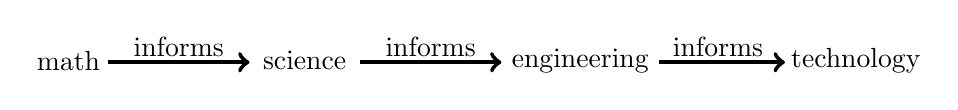
\begin{tikzpicture}
                    \node [align=center] at (0.0, 0.02){math};
                    \draw [ultra thick, ->] (0.5, 0) -- (2.3, 0);
                    \node [align=center] at (1.4, 0.2){informs};
                    \node [align=center] at (3.0, 0.02){science};
                    \draw [ultra thick, ->] (3.7, 0) -- (5.5, 0);
                    \node [align=center] at (4.6, 0.2){informs};
                    \node [align=center] at (6.5, 0.02){engineering};
                    \draw [ultra thick, ->] (7.5, 0) -- (9.1, 0);
                    \node [align=center] at (8.25, 0.2){informs};
                    \node [align=center] at (10, 0.02){technology};
                \end{tikzpicture}
            \end{figure}
                
            However, you'll also find that philosophy informs all of these, and is informed by all of these. The creative arts, like philosophy, is informed by all 4 of these, but tends towards informing only engineering and technology.
                
            This does not mean that mathematics and science is not creative, but it's often misunderstood that because mathematics is so rational, that it's not creative. It takes a lot of creative thinking and intuition, along with rational thought, in order to come up with mathematical proofs, and it is for this reason, and the connections to other fields, that creative arts is a necessary endeavour for anyone learning STEM.
                
            In fact, this is precisely the argument for STEAM.
                
            It must be stated more clearly, because the previous statement may not be clear enough: creative thinking, intuition, and rational thinking are \textbf{all} required for work in each of these fields of study, in concert with each other. Rational thinking does not promote mathematics and science alone. Intuitional thinking will almost certainly lead to falsehoods in these fields, if not matched with rational thinking.
                
            In this sense, creative thinking can be seen to be exploration, finding solution-after-solution, intuitive thinking can be seen to point the creative thinking along, but the rational thinking is the filter that finds the solutions that actually work.
                
            So, you will benefit all of these parts of your mind, including the part of you that is disciplined and builds grit. This will happen by mere practice and use, much like a muscle being used over-and-over getting bigger, and capable of handling more.
                
            Mathematics and the sciences change how you look at the world around you, but it doesn't make you a better person.
        \end{subsection}
        
        \begin{subsection}{The Danger in Strength}
            Philosophy has a long history of beneficial usage and of dangerous misuse. Philosophy may be the most important, but the most dangerous subject matter that a mind can consume. Philosophy has been used to free people as well as enslave people. The philosophical concept of moral or ethical \emph{justification} has been used both to protect and to kill.
            
            In effect, every argument about whether or not human beings are ready for a specific technology is actually a question of whether or not human beings are philosophically mature enough, and is captured in the following quotes:
            
            \begin{quote}{Jason Silva}
                Technology is, of course, a double-edged sword. Fire can cook our food but also burn us.
            \end{quote}
            
            \begin{quote}{Christian Lous Lange}
                Technology is a useful servant, but a dangerous master.
            \end{quote}
            
            \begin{quote}{B. F. Skinner}
                The real problem is not whether machines think, but whether people do.
            \end{quote}
            
            Replace ``technology'' with ``philosophy'' in the first two quotes, and you may begin to understand what it is that I'm claiming. Other quotes are a bit more direct:
            
            \begin{quote}{Martin Luther King, Jr}
                Nothing in all the world is more dangerous than sincere ignorance and conscientious stupidity.
            \end{quote}
            
            \begin{quote}{George Bernard Shaw}
                Beware false knowledge; it is more dangerous than ignorance
            \end{quote}
            
            \begin{quote}{Confucius}
                Real knowledge is to know the extent of one’s ignorance
            \end{quote}
            
            Oftentimes, it is exactly those strengths that serve as one's weaknesses, but that is not to say that having a strength necessarily creates weakness in that area. It benefits us to understand how strengths become weaknesses. 
    
            Philosophy, like technology, is good or bad, depending on how it's used, and depending on how well it's understood, and based on what principles one chooses to work from.
                
            In fact, the call-to-action I give each of you, before you start this endeavour is:
            \begin{itemize}
                \item Use your observations and experiences to help you understand your world
                    
                \item Uproot misperceptions and misunderstandings that come from a partial understanding of the first
                    
                \item Apply your understanding of the world to better your world and the world of others, as you see fit
            \end{itemize}
        \end{subsection}
        
        \begin{samepage}
            \begin{subsection}{Perceptions and Misperceptions of Philosophy, Mathematics, and Science}
                There are multiple misperceptions of about various fields of study, such as:
                \begin{itemize}
                    \item Mathematics
                    \begin{itemize}
                        \item It's not a creative field
                        \item It's the study of numbers
                        \item It's already finished (there's no new math to be had)
                        \item There are no jobs for mathematicians
                    \end{itemize}
                    
                    \item Science
                    \begin{itemize}
                        \item It's done by elite people who have no connection to reality
                        \item It's a collection of statements that are considered ``the truth''
                        \item It doesn't help ``real people''
                    \end{itemize}
                    
                    \item Software Development
                    \begin{itemize}
                        \item It's all copy-and-paste
                        \item Computers will be programming themselves soon
                        \item It's an easy desk-job with little pressure
                    \end{itemize}
                        
                    \item Economics
                    \begin{itemize}
                        \item It's the study of money
                        \item It's all psychology (which contradicts the first claim)
                    \end{itemize}
                \end{itemize}
            \end{subsection}
        \end{samepage}
            
        All of these claims are caricatures of the fields of study, or of the people who do work in those fields, and are not just oversimplifications, but are outright wrong if one were to actually follow these people around.
            
        Much the same misrepresentation occurs in all fields of study and all fields of work. These misrepresentations continue throughout the centuries as populism attempts to change the view of these subjects.
            
        The history of this populism is understood, because in history, fields such as these could only be achieved by the educated and the rich, and those people would not understand those who worked with their hands. Therefore, a schism occurred between those who used their minds, and those who used their hands, based on a classism that is not yet resolved.
            
        A shift has been occurring over the last few centuries though, especially as education has become more universal, allowing people to spend part of their lives in service, part of their lives in manual labor, part of their lives studying, and part of their lives working with their minds, and it's not certain that a person in any particular job has any particular experience.
            
        In this regard, philosophy has always been misrepresented, and you may hear things like:
        \begin{enumerate}
            \item Philosophy, like mathematics, has been completed, or it has produced all of the results and discoveries that it can
                
            \item Philosophy is useless, ungrounded, and a waste of a person's education
                
            \item Philosophy is nebulous, vague, and done by people who are out-of-touch with the real-world
                
            \item Philosophy opposes, is not supported of, or is somehow separate from science
        \end{enumerate}
            
        Nothing could be further from the truth on all of these grounds. Mathematics, and philosophy, are coming up with new discoveries all the time, and including applications to previous discoveries. Philosophy, especially the interest of how we come to know things, forms the basis for both mathematics and the sciences.
    \end{section}
    
    \begin{section}{What is Philosophy, and Why Should We Care?}
        Philosophy is typically introduced by discussing what it means, and where it comes from. We focus so much on the Greek philosophy, but philosophy, mathematics, and science has been growing in all cultures for millennia, and can be found as early trial versions of these subjects in ancient books all over the world.
            
        The word ``philosophy'' is a word from ancient Greek φιλοσοφία (\emph{philosophía}), which has 2 roots:
        \begin{itemize}
            \item φίλος (phílos meaning “loving”)
            \item σοφία (sophía meaning “wisdom”)
        \end{itemize}
            
        However, that only scratches the surface, and tends to lead to the conclusion that “philosophy is in every query”. Although this is technically true, it does little to give anyone any clue to what philosophers actually do, and why it’s important.
            
        In some ways, philosophy is the process of exploring one’s thoughts, asking ourselves, “why do I think this way?”
            
        Specifically, philosophers have certain question that all philosophy branches out from:
            
        \begin{figure}[ht]
            \centering
            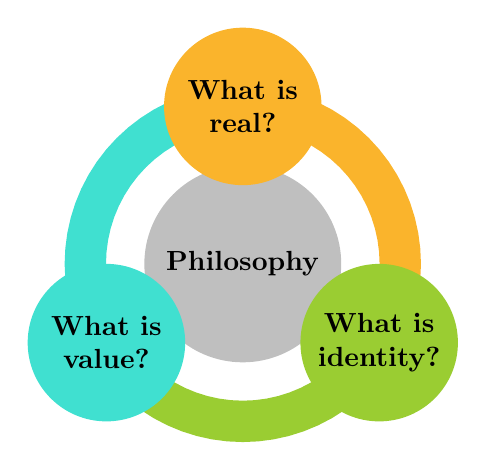
\begin{tikzpicture}
                \fill [lightgray]   (0,0) circle (12.5mm);
                \node [align=center] at (0, 0) {\textbf{Philosophy}};
                \draw [Dandelion,line width=5.25mm,domain=-30:90] plot ({2*cos(\x)},     {2*sin(\x)});
                \draw [YellowGreen,line width=5.25mm,domain=210:330] plot ({2*cos(\x)},     {2*sin(\x)});
                \draw [Turquoise,line width=5.25mm,domain=90:210] plot ({2*cos(\x)},     {2*sin(\x)});
                \fill [Dandelion] (0,2) circle (10mm);
                \fill [YellowGreen] ( 1.732,-1) circle (10mm);
                \fill [Turquoise]   (-1.732,-1) circle (10mm);
                \node [align=center] at ( 0.000, 2) {\textbf{What is}\\\textbf{real?}};
                \node [align=center] at ( 1.732,-1) {\textbf{What is}\\\textbf{identity?}};
                \node [align=center] at (-1.732,-1) {\textbf{What is}\\\textbf{value?}};
            \end{tikzpicture}
            \caption{The 3 Proposed Root Questions of Philosophy.}
            \label{fig:ThreePhilosophicalQuestions}
        \end{figure}
            
        Here though, these 3 questions feed off of each other. For instance, 
        \begin{itemize}
            \item Is it possible to seek truth without asking what methods of truth-seeking that we value?
                
            \item If something exists (if it’s “real” or “true”), can we identify it?
                
            \item If we change something (identity) does it change value?
        \end{itemize}
            
        In fact, these three questions spawn multiple branches of study, some of which are considered philosophical in modern times still, others may appear, on the surface, as if they are something separate from philosophy.
            
        \begin{subsection}{What is Real?}
            Epistemology relates to the question, “How do we know what we know?”. The study     of epistemology has given us logic (forming the foundations of mathematics),     the Scientific Method (forming the foundations of science), and gives us     mechanisms for us to understand beliefs by asking:
                
            \begin{itemize}
                \item What does it mean to know something?
                \item Can anything be known for certain? 
                \item How much confidence can we have in something?
                \item What is the process that we come to know things?
                \item What does it mean to know things?
                \item What is a belief?
                \item Can we justify our beliefs? (\textbf{critical reasoning})
                \item What is the relationship between beliefs and knowledge?     (\textbf{doxastic logic})
            \end{itemize}
        \end{subsection}
            
        \begin{subsection}{What is Identity?}
            In philosophy, we talk about \textbf{discernibility}, which lets us ask, “if two things share all the same properties, are they the same thing?”. We use this in mathematics to present two things being equal. In science, we identify phenomena that interest us. In our lives, we discuss personal identity, social identity, and even discuss the human identity. In many ways, the philosophical focus on definitions and on meanings are directly related to identifying concepts, and coming to agreement on concepts, in order to help discuss.
                
            It leads us to questions like:
                
            \begin{itemize}
                \item What does it mean for two things to be the same, and does that change over time or based on the context?
                \item If I replace every component with an identity component, is it the same thing (Interchangeability and compatibility)?
                \item Are we the same person from one moment to the next?
                \item Is any object the same from one moment to the next?
                \item How do we relate to and do we identify with our city, our culture, and/or our nation?
                \item What does it mean when things are “almost alike” or similar? And do similar things share similar properties?
            \end{itemize}
        \end{subsection}
        \begin{subsection}{What is Value?}
            The notion of \textbf{value} or \textbf{worth} is also of central concern, as it allows us to compare two things. This is also of central concern in mathematics as it allows us to make statements about relationships between things. It is of concern in modern politics, when discussing the value of citizens and whether or not they feel valued. We discuss \textbf{aesthetics} as the study of those things that attract our senses. We discuss \textbf{ethics} through the value of actions. It leads us to questions like:
                
            \begin{itemize}
                \item What does it mean to compare two things?
                \item Why do things cost what they do?
                \item What do individuals value, and why?
                \item What do societies value, and why?
                \item Is something practical worth more than something else? What makes it practical?
                \item What is fairness and justice?
            \end{itemize}
        \end{subsection}
        \begin{subsection}{What is the Relationship Between Value and Identity?}
            When questions about both value and identity come together, we usually start to ask about purpose, and
            \begin{itemize}
                \item Is there a purpose to the existence of the universe? What is the purpose?
                \item Is there a purpose to my existence? What is the purpose? Do I create my own purpose?
                \item Am I a valued part of my community? Why or why not?
                \item What is fair when it comes to treatment of different people?
                \item How does interchangeability relate to comparison? If I interchange components for something newer, is it better?
            \end{itemize}
        \end{subsection}
        \begin{subsection}{What is the Relationship Between Value and Truth?}
            This is the intersection of the two questions that lead us to asking questions like:
            \begin{itemize}
                \item How do we value the various means of obtaining knowledge?
                \item How do people value methods of communicating knowledge and beliefs?
                \item Whose testimonies do we believe and why?
                \item Can there be an absolute, top-level truth, by which all other truths are measured?
                \item Can there be a best moral code, by which all other moral codes are measured?
            \end{itemize}
        \end{subsection}
        \begin{subsection}{What is the Relationship Between Identity and Truth?}
            Regarding identity and truth, we may get some interesting questions about ourselves and:
            \begin{itemize}
                \item What are we? (i.e. what makes us human, or what makes us different?)
                \item Where do we come from?
                \item Why does anything exist at all?
                \item How do we relate to our perceptions, and vice versa?
                \item What does it mean to “exist”?
                \item What does it mean to be “real”?
                \item What is reality?
                \item What is the mind?
            \end{itemize}
        \end{subsection}
        \begin{subsection}{What is the Relationship Between All 3?}
            Finally, we can consider all 3 together:
            \begin{itemize}
                \item Is there something bigger than us?
                \item What is out there, beyond what we can perceive?
                \item How did this universe come to exist? (\textbf{cosmology})
                \item What is the greatest possible mind? Must a creator exist? (\textbf{theology})
            \end{itemize}
        \end{subsection}
            
        \begin{subsection}{Categorizing the Questions into Branches}
            Many of these questions have been placed into various categories:
            \begin{itemize}
                \item That reason can be a source of knowledge (\textbf{rationalism}) allowed us to create logic, and logic continues to refine the foundations of mathematics (classically called, “the formal sciences”)
                    
                \item Critical thinking, using our senses as a source of knowledge (\textbf{empiricism}), building confidence through experimentation (\textbf{verificationism}), and filtering in only those things that we can derive from these sources (\textbf{positivism}) refines the scientific method, which gives us science (classically called, “the physical sciences”)
                
                \item Questions about value form the basis for \textbf{Value Theory}, and include subbranches like: ethics, aesthetics, and axiology (moving into application through economics and politics)
                    
                \item Questions about existence and reality form the basis of \textbf{Metaphysics}, and include subbranches like: theology, religion, and ontology 
                    
                \item Questions about how we do philosophy form the basis of \textbf{Metaphilosophy}
            \end{itemize}
        \end{subsection}
    \end{section}
    
    \begin{section}{Philosophical Discussions}
        So, you thought that this book was going to be about mathematics. Why, then, are we learning philosophy? Well, it turns out that philosophy is the parent of almost every subject studied in any formal education. 
            
        Given that we have asked about reality, science is a formal discipline of the philosophical position called empiricism, allowing us to enter into discussion about those areas of discussion that can be observed and measured with repeatable results. However, as positions go, science is limited to such discussions.
            
        Foremost, we are interested in mathematics in this book, but we will only really get there by discussing the roots of mathematics. Also, in order to understand it, we will do best when we can also link our study to various other areas as well. The most interesting part is how these things link.
            
        \begin{figure}[ht]
            \centering
            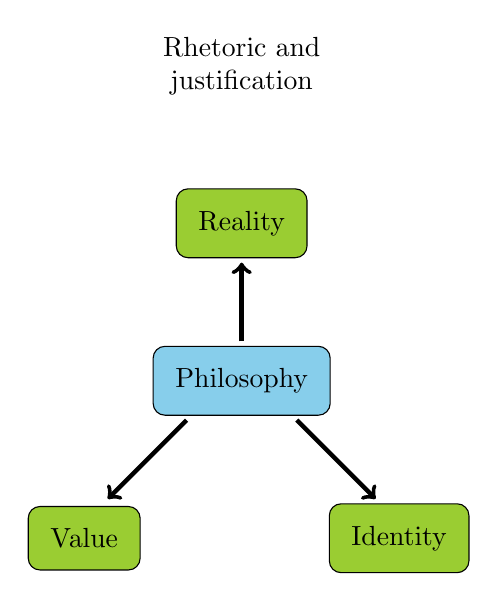
\begin{tikzpicture}
                \node [align=center,draw=black,fill=SkyBlue,thin,inner sep=8pt,rounded corners=.15cm] at (0.0, 0.0) {Philosophy};
                
                \node [align=center,draw=black,fill=YellowGreen,thin,inner sep=8pt,rounded corners=.15cm] at (0.0, 2.0) {Reality};
                
                \node [align=center] at (0.0, 4.0) {Rhetoric and\\justification};
                
                \node [align=center,draw=black,fill=YellowGreen,thin,inner sep=8pt,rounded corners=.15cm] at (-2, -2.0) {Value};
                
                \node [align=center,draw=black,fill=YellowGreen,thin,inner sep=8pt,rounded corners=.15cm] at ( 2, -2.0) {Identity};
                
                \draw [ultra thick, ->] ( 0.0, 0.5) -- (0.0, 1.5);
                \draw [ultra thick, ->] (-0.7,-0.5) -- (-1.7, -1.5);
                \draw [ultra thick, ->] ( 0.7,-0.5) -- ( 1.7, -1.5);
                %\node [align=center] at (0.0, 0.02){math};
                %\draw [ultra thick, ->] (0.5, 0) -- (2.3, 0);
                %\node [align=center] at (1.4, 0.2){informs};
                %\node [align=center] at (3.0, 0.02){science};
                %\draw [ultra thick, ->] (3.7, 0) -- (5.5, 0);
                %\node [align=center] at (4.6, 0.2){informs};
                %\node [align=center] at (6.5, 0.02){engineering};
                %\draw [ultra thick, ->] (7.5, 0) -- (9.1, 0);
                %%\node [align=center] at (8.25, 0.2){informs};
                %\node [align=center] at (10, 0.02){technology};
            \end{tikzpicture}
        \end{figure}
            
        \begin{figure}[H]
            \centering
            \includegraphics[scale=0.65]{PhilosophicalIntroduction/ConnectionsToPhilosophy.png}
            \caption{Connections of Various Fields to Philosophy.}
            \label{fig:ConnectionsToPhilosophy}
        \end{figure}
            
        \begin{subsection}{Rhetoric and Justifying Beliefs}
            It's important to understand that much of our mental sophistication revolves around explaining ourselves to others, whether that be in regards to giving them a mental image of what we have seen, explaining how something works, to justifying our reasons for doing something.
                
            Jonathan Haidt gave us the analogy of our minds being of a human rider on top of an elephant, whereas the rider is the rational mind, and the intuition is the elephant. We are so good at justifying our actions to others, that we often justify things we have done to ourselves, even when we know better (e.g. ``I can eat that whole chocolate cake, because I've done so well on my diet this week.'').
                
            Our written Greek philosophy seems to start with regards to \textbf{rhetoric}, as the ``art of discussion'', developing the communication skills to discuss philosophical positions.
                
            Rhetoric was often divided into:
            \begin{itemize}
                \item \textbf{Emotional} appeals, intended to speak directly to the mind's elephant. These appeals are often highly effective, if sometimes manipulative in their usage.
                    
                \item \textbf{Authoritative} appeals, intended to invoke the authority of the speaker, through their experience or due to their character-history of truthfulness.
                    
                \item \textbf{Rational} appeals, intended to speak directly to the rider of the elephant, who is capable of mapping out a direction for the elephant to travel, if the rider can ever get the elephant to listen.
            \end{itemize}
                
            We may be used to hearing the word rhetoric in political discussions (such as ``inflammatory rhetoric''), but oftentimes the person using the word doesn't mean it with the nuance of the philosophical meaning. Instead, philosophers would deem what politicians are doing \textbf{polemic}, which is emotional arguments intended to reduce confidence in and incite fear of an opponent.
                
            It should be obvious that mathematics and the sciences are filled with logical appeals, and as such, this book will be filled with them as well. However, it's also recognized that the intuition must be brought on board as well. 
                
            Finally, the authoritative appeals should be mostly unused in any discussion of mathematics. There is no for a teacher to use appeals to authority, saying things like ``it just works this way''. The only authoritative appeals will be the usage of already defined and commonly used standards for writing that may be brought up. However, even those should be backed with arguments for rational reasons why.
                
            \begin{subsubsection}{Some Definitions}
                
                \begin{definition}
                    An \textbf{interlocutor} is a person that is taking part in a dialog.
                \end{definition}
                    
                \begin{definition}
                    A \textbf{proposition} is a statement is possibly true or false.
                \end{definition}
                    
                \begin{definition}
                    A \textbf{premise} is a proposition for consideration, sometimes asserted as true by the interlocutor, and sometimes as a condition for the context of the argument.
                \end{definition}
                    
                \begin{definition}
                    A \textbf{conclusion} is a proposition that is the end result that the interlocutor reaches starting from the premises.
                \end{definition}
                    
                \begin{definition}
                    An \textbf{argument} is a series of propositions, structured such that the premises lead to a conclusion. Furthermore, a more general meaning of this word may be a process of reasoning.
                \end{definition}
                    
                \begin{definition}
                    A premise taken as a condition, usually in regards to an investigation is called a \textbf{hypothesis}.
                \end{definition}
                    
                \begin{definition}
                    A \textbf{philosophical position} is a collection of premises that an interlocutor is arguing from.
                        
                    It is often called a \textbf{philosophical theory}, which can cause confusion with the significantly different meanings taken by scientific theory and mathematical theory. 
                        
                    The everyday usage of the word ``theory'' is probably best identified as ``hypothesis''.
                        
                    Due to this confusion, the word position will be preferred in this book.
                \end{definition}
                    
                \begin{figure}[ht]
                    \centering
                    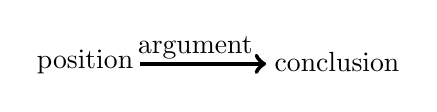
\begin{tikzpicture}
                        \node [align=right] at (0.0, 0.02){position};
                        \draw [ultra thick, ->] (0.7, 0) -- (2.3, 0);
                        \node [align=center] at (1.4, 0.2){argument};
                        \node [align=left] at (3.2, 0.02){conclusion};
                    \end{tikzpicture}
                    \caption{Relation between position (premises), argument, and conclusion}
                \end{figure}
                    
                \begin{definition}
                    For the sake of comparison, a \textbf{life stance} is a philosophical position that one takes, according to their worldview, which informs their beliefs, their thoughts, and their behavior.
                        
                    This is stated separately, since a life stance differs from a philosophical position.
                \end{definition}
                    
                \begin{definition}
                    A \textbf{Devil's Advocate} is a person that argues from a position that differs from their life stance, in order to better understand their own position, and the position of others.
                \end{definition}
                    
                \begin{definition}
                    \textbf{Skepticism} is the act of reserving belief for future evidence.
                \end{definition}
                
                \begin{definition}
                    \textbf{Belief revision} is the act of modifying one or more premises that make up a position, due to new evidence.
                \end{definition}
            \end{subsubsection}
            
            \begin{subsubsection}{What Forms a Worldview}
                At this point, I'm going to present what follows as a position, setting the rest of the book up for discussions on logical reasoning.
                    
                \begin{remark}
                    This position I am starting from, regarding worldviews, is not scientific, is not based on psychological evidence, and is likely just an approximation of how worldviews actually work.
                \end{remark}
                    
                \begin{figure}[ht]
                    \centering
                    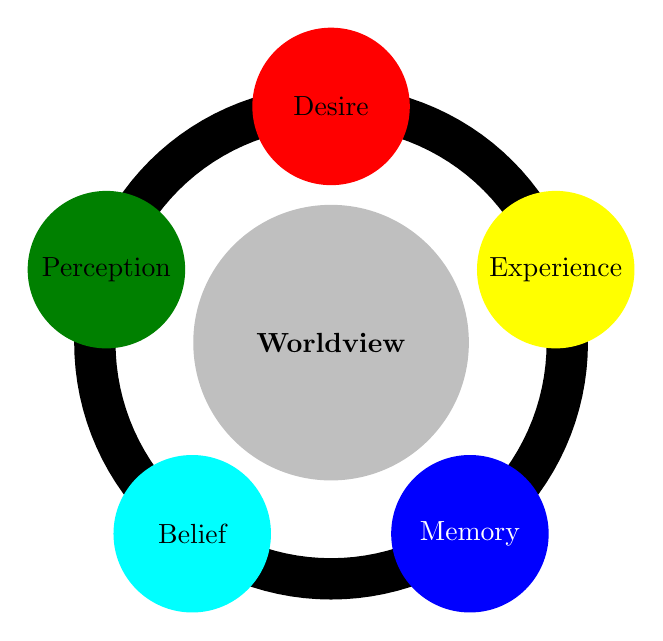
\begin{tikzpicture}
                        \fill [lightgray] (0,0) circle (1.75cm);
                        \node [align=center] at (0, 0) {\textbf{Worldview}};
                            
                        \draw [Black,line width=5.25mm,domain=90:162] plot ({3*cos(\x)}, {3*sin(\x)});
                        \draw [Black,line width=5.25mm,domain=162:234] plot ({3*cos(\x)}, {3*sin(\x)});
                        \draw [Black,line width=5.25mm,domain=234:306] plot ({3*cos(\x)}, {3*sin(\x)});
                        \draw [Black,line width=5.25mm,domain=306:378] plot ({3*cos(\x)}, {3*sin(\x)});
                        \draw [Black,line width=5.25mm,domain=378:450] plot ({3*cos(\x)}, {3*sin(\x)});
                            
                        \fill [Red]   ( 0.000000, 3.000000) circle (10mm);
                        \fill [Green] (-2.853170, 0.927051) circle (10mm);
                        \fill [Cyan]  (-1.763356,-2.427051) circle (10mm);
                        \fill [Blue]  ( 1.763356,-2.427051) circle (10mm);
                        \fill [Yellow]( 2.853170, 0.927051) circle (10mm);
                            
                        \node [align=center,text=black] at 
                        ( 0.000000, 3.000000) {Desire};
                        \node [align=center,text=black] at 
                        (-2.853170, 0.927051) {Perception};
                        \node [align=center,text=black] at 
                        (-1.763356,-2.427051) {Belief};
                        \node [align=center,text=white] at 
                        ( 1.763356,-2.427051) {Memory};
                        \node [align=center,text=black] at 
                        ( 2.853170, 0.927051) {Experience};
                    \end{tikzpicture}
                    \caption{Relation between position (premises), argument, and conclusion}
                \end{figure}
                    
                The first question someone may have looking at the components of a person's worldview that I listed is that experience, memory, and belief are all the same thing. However, my argument is that we experience all the time, but our beliefs color how we interpret the memories associated with those experiences.
                    
                In this sense, we reexperience things through our memory, but it doesn't mean that it feels the same each time.
                    
                It may seem strange that I put desire in with the rest of these, because it appears that the rest of these relate to knowledge, but that desire is completely unrelated. However, we already know that desires change how we perceive things, making us more or less perceptive of our failures or successes, or how other people act.
                    
                The point of all of this is to say that our memories are fallible, because they change. Our perceptions are fallible as well, and so, we cannot always trust our worldview.
            \end{subsubsection}
                
            \begin{subsubsection}{What Sources of Information do you Value?}
                In the discussion of rhetoric, we talked about 3 different types of arguments: emotional, authoritative, and rational.
                    
                However, these are only the methods of transference of information from one person to another, and misses an important source of information: experience.
                    
                We tend to regard experience as the most valued source of information, but as we discussed in regards to the worldview, our perceptions of experiences are often incomplete, and sometimes even wrong.
                    
                Most people, naturally value emotional, authoritative, experiential, intuitive, and rational information sources to some level or another, because we naturally recognize that there are failings with putting all of our trust in any one of them: emotions can sometimes be erratic, people sometimes lie, our perceptions often deceive us, our intuitions are often wrong, and we often don't have enough information to come to a rational conclusion.
                    
                However, there are things that we can do to refine when we use each, and what we can be said about each source of information.
                    
                Firstly, it's important to note that rational arguments begin as intuitive arguments. Humans have an intuitive ability to recognize cause-and-effect, allowing us to determine how things work, and often change how things work to our favor. This recognition of the pattern of cause-and-effect is what leads us to logic, and rational thinking is the disciplined use of this logic. 
                    
                In fact, the discipline is what separates intuition from rational thinking. We follow through with our intuitions to see if they fail.
                    
                Second, the relationship between emotions and intuition are also important. Purely rational thinking is devoid of creativity, can get stuck in analysis, and therefore absent problem solving ability. However, purely intuitive thinking cannot weed out those ideas that won't work, and will naturally try things that are not logically sound, usually wasting their own and other people's time.
                    
                First, let's get more detailed how these each operate as a source of information:
                \begin{itemize}
                        
                    \item Authoritative sources
                    \begin{itemize}
                        \item \textbf{Witnesses} can provide accounts of events
                        \item Parents and teachers often provide us tons of information
                    \end{itemize}
                    \item Experiential sources
                    \begin{itemize}
                        \item Your \textbf{senses} give you access to the world around you and are your connection to it
                        \item When your senses act together they create an \textbf{empirical} view of the world
                        \item This effectively places you as an authority over your own worldview
                        \item Demonstrations from other individuals can help communicate subject matter
                    \end{itemize}
                    \item Emotional and Intuitive sources
                    \begin{itemize}
                        \item Emotions can point us to how our intuitions react to specific experiences
                        \item Gut feelings can tell us things about our world, and are frequently part of our mental pattern-matching capabilities.
                        \item It is via these gut feelings that we are capable of walking, knowing where to place each foot as we move
                        \item The intuitive is unconscious, but quick to form conclusions
                    \end{itemize}
                    \item Rational sources
                    \begin{itemize}
                        \item We use logic and probability to determine whether or not something is possible
                        \item We use analogy to compare and contrast things that we know against things that we do not know
                    \end{itemize}
                \end{itemize}
                    
                We know that authorities can lie, and that witnesses can't always trust their memories. Likewise, we cannot always trust our senses, nor our memories. Our emotions and intuitions are often wrong. Also, we can misuse logic, probability, and analogy.
                    
                In seeking information that we can trust, it seems like we are out of luck, but through careful inspection, we can begin to clear out the mess.
                        
                Regarding rational and intuitive thought, if we learn how to properly use logic and to understand our own biases, we can balance intuition with rational thinking, by allowing intuition to come up with hypotheses, and cutting through the wrong ones via rational thought. We can learn how where rational thinking works, and how sometimes fails us.
                    
                Regarding experience, we can learn about our own psychology, and also through our biases, determine when we can trust our senses and our experiences. We can determine whether multiple memories working together with evidence can corroborate our hypotheses.
                    
                Regarding authorities, \textbf{Subject Matter Experts} are people who are experienced in a subject matter and have a record of insightful discussions, and as long as they have no motive to lie to us, information inside their area of expertise can be trusted.
                    
                From there, we can actually learn what authorities know, how they came to their conclusions, and come to conclusions ourselves via experience and rational thinking.
                    
                So, it's important to think about how and why you value the sources of information that you do, how and why they can fail you, and how to effectively work through them.
            \end{subsubsection}
                
            \begin{subsubsection}{Epistemology}
                The study of what we know and how we come to know it is called \textbf{epistemology}. It is extremely important in the realm of mathematics and the sciences to understand epistemology, 
            \end{subsubsection}
            \begin{subsubsection}{Rigorous Communication}
                Furthermore, most of this communication between experts requires that the words they use are well-understood. We have definitions for words that we use all the time, but often words in a particular \emph{subject matter} have explicit definitions which differ from how they are used in everyday speech.
                    
                Let's consider one of the most problematic words in use today. The word \textbf{theory} from the ancient Greek θεωρία (``theoria'') was contrasted to πρᾶξις (``praxis'' where we get the word ``practice''). The theory behind something was the contemplation regarding how an activity works, and the praxis was the act of doing it. Therefore, theory was used to improve the praxis, but praxis was used to improve the theory.
                    
                This contrasting terminology between the two is why we still have phrases like ``that's works in theory, but not in practice''. However, the meaning of theory in our everyday life is not necessarily how it is used elsewhere:
                    
                \begin{itemize}
                    \item \textbf{Theory (science)} -- a hypothesis which is confirmed by repeated and thorough experimental observation to provide reliable predictions
                    
                    \item \textbf{Theory (mathematics)} -- the collection of premises and conclusions related specific mathematical structures
                        
                    \item \textbf{Theory (philosophy)} -- the collections of premises and conclusions specific to an area of philosophical pursuit (also called a philosophical position).
                        
                    \item \textbf{Theory (everyday speech)} -- a proposed explanation serving as a hypothesis
                \end{itemize}
            \end{subsubsection}
                
                
        \end{subsection}
        \begin{subsection}{Ontology and the Mathematics of Identity, Equality, and Equivalence}
            Discernibility
            Distinguisibility
            Interchangeability
            Identical
                
            \begin{subsubsection}{Definitions}
                In every field of study, we have to be extremely careful what it is we mean when we say something, and aim to avoid
                    
                In mathematics, we often define something, to use in a context (a scope of discussion) and when we are done, we stop meaning it the same. In speech, we do this often with pronouns. For instance, ``Caleb left work. He wasn't feeling that well.''. We immediately know that `He' in the sentence refers to Caleb. In this case, with English, we didn't even specifically define that we'd use `He' this way.
            \end{subsubsection}
                
                
            \begin{subsubsection}{Isomorphisms}
                \begin{definition}
                    The word \textbf{isomorphism} has a formal definition that we will cover later in Category Theory. Philosophically, it can be thought best to first recognize that mathematical objects are conceptual, not physical, and we can argue only that two objects constructed exactly the same way (structural identity) are identical. However, as we have said, two objects can be constructed in 2 different ways and behave as if they are the same object. These objects then have interchangeability between them.
                    
                    An isomorphism focuses, not on identical constructions (what the objects ``are''), but on identical behaviors (what the objects ``do''), and more specifically, that they adhere to the same ``legal contracts'' we call axioms.
                    
                    The word isomorphism (iso- ``same'', -morphism ``form'') is an effective ``equality between types of things''. 
                \end{definition}
                
                An example would be the 2 identical definitions for the number 1:
                \begin{enumerate}
                    \item The natural number comes after 0
                    \item The unique natural number that allows us to multiply any number by itself and result in the same number
                \end{enumerate}
                
                Both of those definitions for 1 focus on what it does, but the first definition is closer to the actual construction of 1 than the second. The two definitions are isomorphic to each other.
                    
                Furthermore, we have the Univalence Axiom, which binds multiple mathematical fields together, in the same way that René Descartés bound algebra together with geometry when he noticed that we can put things on a grid. The proposal of the Univalence Axiom first observed that equivalence (structural identity) implies isomorphism(interchangeability), but the true observation was that an isomorphism was interchangeable with an equivalence.
                
                Now, that's not being fully honest, and yet it is at the same time. A good philosopher will think to themselves, ``you didn't use the word `equivalence' the same way in both of those sentences'', and that philosopher would be right.
                
                I started the discussion talking about identical constructions (what objects ``are''),and obviously, two things cannot be equivalent if they do not have identical constructions. However, equivalence doesn't have to mean identical constructions.Mathematicians often define equivalence based on interchangeability in the same sense as the following analogy:
                
                \begin{quote}
                    A ``Gizmo'' machine has a component called a ``doohickey''. If I can take the doohickey out and replace it with another doohickey, they are interchangeable. If I can replace the Gizmo with another Gizmo, and use the same doohickey in both, then the Gizmo itself is fungible (interchangeable with other things that use components). If any doohickey can go in any Gizmo, then the differences between each doohickey is indiscernible.
                \end{quote}
                
                So, we get an isomorphism between algebraic equations and geometry from Descartés. From Euler we'll see how trigonometry, calculus, and complex numbers relate. However, here we use this opportunity to note that there is an isomorphism between paths, logic,partial orders, computation (and computer science), and tons of things we may get to later, just from Vladimir Voevodsky's Univalence Axiom.
                
                Finally, I have mentioned Axioms as ``legal contracts for mathematical structures''.You may be asking, what structure do we assume Univalence for? We will eventually get into Category Theory, and that will help combine all the world of mathematics together for us.
                
                So, it helps to understand that equality has context, just as isomorphism has context, and we may discuss various types of equalities.
            \end{subsubsection}
                
            \begin{subsubsection}{Natural Numbers are not Non-negative Integers}
                Never does the distinction and non-distinction matter as much as how we teach the number classifications. We have probably been taught that we can identify integers as allowing for negative numbers, and that every natural numbers \textbf{is} an integer.
                    
                This notion of \textbf{is} refers to our isomorphism from earlier. We can construct integers, and we can construct natural numbers, and we will construct them later, but the statement ``\textbf{is}'' used above must be understood to mean that we can get an integer from a natural number, and take that same integer and find a natural number that matches it. That is what it means to ``be the same''.
            \end{subsubsection}
        \end{subsection}
    \end{section}
\end{chapter}
    %\include{Classical Logic}

\documentclass[11pt,twoside,letterpaper,fleqn,parskip=full]{book}

\input{structure}

\makeglossaries
\begin{document}
\newglossaryentry{LawsOfThought}
{
    name={Laws Of Thought},
    description={The 3 laws of classical logic, written down by Aristotle}
}

\newglossaryentry{ClassicalLogic}
{
	name={Classical Logic},
    description={Basic 2-value logic with logical implication, and operations AND, OR, and NOT}
}

\newglossaryentry{BooleanDomain}
{
    name={Boolean Domain},
    description={A domain that has 2 possible-values with the interpretation that one element represents true and the other element represents false}
}
\newglossaryentry{ProofByExhaustion}
{
    name={Proof By Exhaustion},
    description={Creating a deductive proof by analyzing every possible value}
}

\newglossaryentry{bit}
{
    name={bit},
    description={A single element of the Boolean Domain, interpreted as either true or false}
}

\newglossaryentry{symmetry}
{
    name={symmetry},
    description={the property of a relation that allows us to swap the items of the relation}
}

\newglossaryentry{proposition}
{
    name={proposition},
    description={a proposition is statement that can have a truth-value}
}

\newglossaryentry{involution}
{
    name={involution},
    description={Any function that when applied twice produces a result the same as the input}
}

\newglossaryentry{PositionalNotation}
{
    name={Positional Notation},
    description={(also called Place-value notation) uses position to represent numbers, such that numbers that come first have a larger value than those that follow}
}
\nocite{*}
%-- TITLE PAGE --

\begingroup
\thispagestyle{empty}
\centering
\vspace*{5cm}
\par\normalfont\fontsize{35}{35}\sffamily\selectfont
\textbf{Mathematics}\\
{\LARGE Mathematics through Intuition and Rigor}\par % Book title
\vspace*{1cm}
{\Huge Nicholas Cooper}\par % Author name
\endgroup

%-- COPYRIGHT PAGE --

\title{Mathematics}

\newpage
~\vfill
\thispagestyle{empty}

%\noindent Copyright \copyright\ 2014 Andrea Hidalgo\\ % Copyright notice

%\noindent \textsc{github.com/FILLLLLLLLTHISSSSSSSOUTTTTT} % URL

%\noindent This book was created>>>>. % License information

%\noindent \textit{First release, August 2018} % Printing/edition date


%\pagestyle{empty} % No headers

\tableofcontents % Print the table of contents itself

\begin{part}{Graphs, Deduction, and Containers}
    \chapter{Directed Graphs}

There have been some issues with teaching mathematics lately, and most of those issues have come about from the lack of certain foundational information that we build up from. There are too many people that think math is the study of numbers, and so it would be good to dispel this view, give a real overview of mathematics, and provide intuitive, rational, and practical discussions as we go.

All of this said, philosophy is paramount to understanding mathematics and science, but we are specifically going to work with understanding some basics through graphs.

\includegraphics[scale=0.55]{01/XMenAvengersFamilyTree.png}

Looking at the directed graph that I provided, this graph relates parents to their biological children. You can see that Magneto was the father to Polaris, to Scarlet Witch, and to Quicksilver. We consider the relationships that are described by the graph:

\begin{itemize}
    \item Child -- identified as those next people by following the arrows
    \item Parent -- identified by following the arrows to the previous people
    \item Descendant -- identified as any person that can be reached by following arrows directly
    \item Ascendant -- identified as any person that can be reached by following arrows backwards
\end{itemize}

Let's look at another directed graph. This graph is a graph of people that follow each other on Twitter.

\includegraphics{01/FollowersOnTwitter.png}

We have Hugo following Gopal and Gopal following Hugo, as represented by two arrows, one going each way between the two. However, it's also the case that there are those that follow a person without being followed back. For instance, Ben follows Damika, but Damika is not following Ben back. 

There is also a cycle in the graph. We have that Damika follows Fawzi, and that Fawzi follows Eleanor, and that Eleanor then follows Damika. This forms a cycle between the 3 of them.

In each of this cases, we are defining relationships between things. Mathematics is a useful tool for describing relationships. Later, we will learn exactly how to construct each of these graphs formally, but for now, the idea of using arrows between objects is a notion that should be fairly intuitive for most people.

As far as definitions go, graphs are drawings that relate objects to each other. A \textbf{directed graph} is drawn with arrows, and it denotes one-way relationships. \textbf{undirected graphs} are drawn with lines, and denotes two-way relationships.

Additionally, when talking about Graph Theory, a \textbf{node} is what we are relating, and the \textbf{edge} is the relationship, usually denoted by an arrow.

We can make an undirected graph from a directed graph by removing the arrowheads, such that every edge is understood to go both directions.

We discern graphs from multigraphs, which may have multiple edges leading to the same nodes.

\includegraphics{01/slopes.png}

In this multigraphs, you can see that there are multiple ways to get from the Bunny Trails to Walkers and Canes. The Kid's Slope is right next to Walkers and Canes, and you can walk back and forth between each other, before going down either to Happy Landing.

You will also notice that every single area has a \textbf{loop} that shows that you can get to where you are from where you are. \textbf{Loops} are edges from a node, back to itself. It seems a bit overkill to put this in, but there are some directed graphs where all nodes have loops, some where no nodes have loops, and there are some directed graphs yet where only some nodes have loops.

Loops make sense when describing paths between things. Loops don't make sense when describing parents, since someone cannot be their own parent. Likewise, with Twitter, you don't really follow yourself, so there are no loops. However, if we were discussing 

The only thing to mention is that you cannot walk your way back up the actual slopes themselves. Of course, not pictured, is the ski lift that can take you back to Summit from Base. So, what is represented is the different ways that you can get to each point on your skis (either by skiing or walking). Because there are multiple paths from Bunny Trails to Walkers and Canes (and from Summit to Steep Gorge), it is a directed multigraphs, not a directed graph.

If our only concern was whether or not we could get from one to the next, and not how many paths there were, then we could remove the extra lines:

\includegraphics{01/slopes2.png}

Compare the multigraphs of the slopes, to the directed graph of the slopes.

So, directed graphs may only have zero or one edge (i.e. "edge or no edge"), in the same direction, between two nodes, and directed multigraphs may have zero or more edges, in the same direction.

Now, with this in mind, this idea of reachability is important in mathematics, and logic. If we have a directed graph and we only care about reachability, we end up with a \textbf{category graph}.

Because we are only interested in reachability, the category graph for the slopes would look like this:

\includegraphics{01/slopes3.png}

In this category graph, we can say that we can reach Bunny Trails from Bunny Trails without having to include the loop itself. Loops are implied in category graphs. Likewise, because a category graph is interested in reachability, we know that we can reach Cat's Claw from Steep Gorge, because we can go through Fun Run to get there.

\chapter{Introduction to Logic}

This is the beginning of understanding logic. Logic starts with this idea of reachability, allowing us to say that, if we are at Steep Gorge, and we can get to Fun Run from Steep Gorge, then we can get to Fun Run.

In logic, when we are talking about reachability, we call it \textbf{deductive closure}, which is the ability to arrive at a \textbf{conclusion} (the target node), based on starting information (the source node), and the relationship (the edge/arrow).

So, let's introduce a category that we usually call a \textbf{rational argument}. We can draw a rational argument in a category graph as well, and work through it.

A \textbf{rational argument} is therefore a collection of \textbf{logical statements} and their relationships.

The usage of the word argument here does not imply some kind of altercation between two people, but is a means to make a claim or justification for why you came to your conclusion.

Let's take a moment, and attempt to make a rational argument. For instance:
\begin{enumerate}
    \item Sprinklers will cause the ground to get wet
    \item Rain will cause the ground to get wet
    \item It rained last night
\end{enumerate}

From this, we have a case where either the first premise or the second premise, can cause our conclusion:

\includegraphics{01/OrCase1.png}

Here, we see the rational argument drawn out. You can see that the phrase, "will cause" has been replaced by an arrow. Often, \textbf{implications} (the logical edges) are due to cause-and-effect relations, but not only is implication much more \textbf{general} (handling many more cases than just cause-and-effect relations), these types of relations don't even form the majority of those that you may use.

Formally, an \textbf{implication} is a relation connecting one \textbf{logical statement} to another logical statement.

However, it's important to notice that the ability for us to discern cause-and-effect relations are probably what gave us the ability to discern other kinds of implications.

Noticing that we have our starting position listed as the 3rd point in our rational argument:

\includegraphics{01/OrCase2.png}

We now look and see what we can reach from there:

\includegraphics{01/OrCase3.png}

We can \textbf{conclude} that the ground is wet. This extends the information that we have, based only on what was there.

We also note the following: each implication is a \textbf{premise}. Likewise, any \textbf{claim} that a logical statement is \textbf{true} is also a premise. Therefore, the relations and our starting information are all premises of a rational argument.

Where we see an implication, or an arrow between two logical statements, we take that to mean that the target statement must be at least as true as the source statement. That is to say that if the source statement is true, then the target statement must be true. Any time we have an implication, this is what the implication is attempting to give us. 

However, because multiple things may have led to the target being true, that the target is true doesn't mean the source is, instead it may have been because of another cause or implication. Notice that, because the ground is wet, does not mean that it was because the sprinklers were on.

Therefore, the relationship is one way.

Usually, it becomes unwieldy to continually use large sentences in our discussion of rational arguments, so much how our graph has replaced the sentences with numbers, we often use symbols to represent our logical statements.

\begin{itemize}
    \item R -- It has rained
    \item S -- The sprinklers ran
    \item G -- The ground is wet
\end{itemize}

In this case, every time we have one of these letters (R, S, or G), we understand them to stand in place of our sentences above.

Then, we end up with the implications:

\begin{itemize}
    \item $R \to G$
    \item $S \to G$
\end{itemize}

And here, we have the arrows pointing to the target G, in both cases. We can look at this and say in English that ``Either the ground is wet because it rained, \textit{or} because the sprinklers ran''.
\begin{tikzcd}[column sep=0.5cm]
    R \arrow[rd] & \ & \arrow[ld] S \\ 
        & G
\end{tikzcd}

Furthermore, the idea that there are 2 options, even makes sense if they are disconnected from anything. Let's consider this: ``We know that either the sprinklers ran, or that it rained.''. Notice that we didn't include the conclusion: ``that the ground is wet''. In this moment, we don't have to, as we are only going to consider the claim that one of these 2 options must have happened.

Now, if we claim to know that one of two options has happened, and then we claim to know that one didn't, then we are stating that the other happened. In our case, we say that ``the sprinklers didn't run'', but since we know at least one of the two statements happened, then we know that ``it rained'' is the correct statement.

This is another form of \textbf{logical inference}. When we know $R \vee S$ and $\neg R \vdash S$. Let's consider another example of this: Tammy and Sahmail own a car. It's reasonable that one of the two of them are the ones driving it. We are hanging out with Sahmail when we see his car go by. It's reasonable to assume Tammy is driving it.

Logically, we get the statements, ``Tammy is in the car or Sahmail is in the car'' and ``Sahmail is not in the car'' therefore ``Tammy is in the car''.

Furthermore, using our implication from before, we can also state, ``If the car is moving, someone must be driving it'' and ``the car is moving'' therefore ``Tammy is driving''.

So, here, we inferred two different (but related) conclusions using two methods. The first method was \textbf{disjunctive elimination}, which eliminated all other possible cases, and \textbf{modus ponens}, which allows us to conclude via implication. 

Now then, we can 


So, along one branch, we can say that if we know $R$ (``it rained''), and we know that $R \to G$, then we can say that $R, R\to G \vdash G$, which tells us what information we extended ($G$). In some ways it ``feels like'' we have ``computed'' $G$ from $R$ and $R \to G$.

The extended information via this implication is called an \textbf{entailment}. The process of extending our information is a rule of inference. We will learn a few rules of inference (ways to extend our knowledge) as we go, but this one is typically called \textbf{modus ponens}, which is Latin for ``

You'll notice that we have discovered that we can express the connective \textbf{or} in logic. In order to understand it from the information that we gave, we know that the ground is wet if it rains, if the sprinklers ran, or both. It's important to understand here that if we are going to be thorough with our definitions, we want or to include both as a case.

If we need to discern between the meaning of ``or'' which includes both and that which excludes both as a cause, we will use the terms ``inclusive or'' and ``exclusive or''. Likewise, we will attempt to use ``either ... or'' when we have a sentence that is going to exclude the combined case.

If we represent this ``inclusive or'' with the following symbol ``$\vee$'' which combines two statements together, then we can say that $R \to G$ with $S \to G$ can be written as $(R \vee S) \to G$. We use the parentheses there to indicate that we want to say that the entire sentence $R \vee S$ is taken as a whole, before we consider it to imply $G$.

You'll notice here that just adding ``or'' into the mix, things got a bit complicated quickly. This is why it's important to discuss \textbf{vocabulary} and to provide \textbf{formal definitions} of things in mathematics, and frankly, in just about any field of work, because the everyday definitions for words usually leave too much to the imagination (they are too ambiguous), and it leaves the two people who are communicating unsure what each is saying.

While we are at it, let's talk about what it means to be ``formal''. In order to understand this word, and the way that it's used, we have to go back to standards of Victorian etiquette. It's not that the word comes from Victorian etiquette, it's much older than that, but it's probably the easiest point-in-time to explain the meaning of the word ``formal'' in terms of how they used the word ``discipline''.

The word ``discipline'' doesn't mean ``to punish'', instead it means something more along the lines of controlled behavior, and following a system of rules. A useful analogy would be to think of the difference between strength and control. You can have a significant amount of strength, but without some control, it becomes impossible to do delicate things.

In this way, our \textbf{intuitions}, the part of our mind that comes up with patterns (strength), requires some focus, the \textbf{rational mind}, to work through those patterns and ideas that may not actually work (control).

So, oftentimes, even though the two seem to be working against each other, creating lots of ideas vs cutting through and removing those ideas that don't work, they are actually complementing each other in a way to ensure that our judgments are correct.

With that in mind, let's discuss where our intuitions may fail us. Consider the following statement, ``If rains, then the ground will be wet.''

We have stated this before as an implication between ``It rains'' and ``the ground will be wet''. However, consider the \textbf{converse}, ``If the ground is wet, then it rained.'' Obviously, we just stated a reason why it the ground can be wet, and yet it has not rained (``the sprinkler case''). Therefore, when working implication we know that the following two statements are not equal to each other logically:


\todo{bring up ``and''}


\begin{itemize}
    \item $ R \to G $
    \item $ G \to R $
\end{itemize}

And in fact, one is wrong. Furthermore, let's also consider the case where we reject both, ``It did not rain; therefore, the ground is not wet'' (i.e. $\neg R \to \neg G$). Again, because the sprinkler could have run, the ground could still be wet. We use the symbol $\neg$ to indicate that we are rejecting the statement.

So, let's talk about the differences between causation and implication. We know that ``the sprinkler running'' is sufficient for ``the ground to be wet''. Therefore, if the ``ground is not wet'' and the ``sprinkler is running'', then our statement that ``when the sprinkler runs, the ground gets wet'' must be wrong. If it is correct, then we must conclude that if ``the ground is not wet'', then the ``sprinkler must not be running''.

Symbolically, this is understood to reverse the arrows, and take the logical negation ($\neg G \to \neg R$). We will discover later the reason that this works, and when we discuss other logic systems, we will even discuss which logic systems it doesn't work for.

For now, we can say that any implication $a \to b$ also implies $\neg b \to \neg a$. For instance, saying ``when 

However, what happens if we have  

\todo{discuss ``and''}

\subsection{Summary of Section}

In this section we learned:
\begin{enumerate}
    \item An \textbf{implication} associates one statement with another, such that one necessitates the other, such as a dependency
    \item A \textbf{disjunction} combines two statements ($P \vee Q$) such that
    \item A \textbf{conjunction} combines two statements ($P \wedge Q$)
    \item An \textbf{inference rule} is a process for extending our information
    \item An \textbf{entailment} is the informational result of applying an inference rule to our deductive argument
    \item \textbf{Modus Ponens} is the inference rule for implication where $P, P \to Q \vdash Q$, meaning ``If P implies Q and we assert P, then we infer Q as well''
    \item \textbf{Modus Tonens} is the inference rule for implication where $\neg Q, P \to Q \vdash \neg P$, meaning ``If P is necessary for Q, and we know Q is false, then P must also be false''
    \item \textbf{Disjunctive Elimination} is the inference rule for disjunctions (``or''), where $P \vee Q, \neg P \vdash Q$, meaning ``If we know P or Q must be true, and P is not true, then Q is true''.
    \item \textbf{Conjunctive Elimination} is the inference rule for conjunctions (``and''), where $P \wedge Q \vdash Q$, meaning ``If we know P and Q, then we must know Q''
\end{enumerate}

\section{Logical Negation, Classical Logic, and Boolean Logic}

Looking at the consequences of \textbf{negation} (which is a word that can mean ``to reject'', among other things), in English, we often consider that double-negation is equivalent to the original statement: ``It's not the case that Sarah didn't take the bus today'' is equivalent to saying, ``It's the case that Sarah took the bus today''.

In \textbf{Classical Logic}, we usually have the case that $\neg \neg P = P$, which is to say that negating the negative of any statement is as true as (=) the original statement. We will later study situations where this doesn't work, and why we may be interested in those cases as well.

So, now we have claimed that there are multiple kinds of logic, those where double-negation results in the original statement, and those where it doesn't.

However, we should be clear what this means and what it doesn't mean in regards to language. Many Latin-based languages make every part of a sentence negative, but this doesn't mean that the other languages aren't working with Classical Logic. Additionally, knowing in English when we switch to other logical systems is not always clear.

Therefore, it helps to ask beforehand, whether you are working within a system where things can be partially true or if they must only be true or false.

With this in mind, Classical Logic only works with these 2 values, and we will show why adding additional values is what causes this double-negation rule to fail.

So, here, we claim that Classical Logic has only 2-values, and so if we just consider statements to either be ``true'' or ``false'', then this is the system we get.

So, we end up needing quite a few more names for all of this than you usually think. For one, the traditional mechanism of describing logic through premises and implication is usually called \textbf{Logiscism}, and the structure that is described using premises and implications is called an \textbf{axiomatic system}.

So, Classical Logic describes a classification of systems that share characteristic properties:

\begin{enumerate}
    \item There are only two values / Double-negation is eliminated $\neg \neg P = P$
    \item Nothing can be both true and false
\end{enumerate}

e



Likewise, 



contrapositive and the ''more true''



Difference between causation and association.
    
\end{part}


\begin{part}{Mathematical Introduction to Philosophy and Logic}
    It may seem strange to start off a book of mathematics with philosophy, but I believe that it's necessary, in order to understand what mathematics is, what it's not, and what it's relationship is to other fields of study, such as the sciences. Furthermore, we want to know why we can consider certain things a source of knowledge and why we can trust certain things.
    
    In fact, this ideas fall into the crux of philosophy -- the most important questions, which lead to the remainder of philosophy. This book is not written to necessarily traditional views, and so this discussion of the \emph{roots of philosophy} will be a source of questions that is not typically a focus had by all philosophers.
    
    There are many branches of philosophy, and this book will focus mostly on logic. The book will contain some foundational material for mathematical and scientific inquiry, and the nature of knowledge itself. A brief introductory presentation will be given for philosophical areas of questioning, such as ethics, the nature of being, and the issues that come from poorly understood philosophical positions. Finally, many areas of questioning that philosophy addresses will be absolutely ignored by this book, due to the focus that this book has on mathematical learning.
    
    \begin{chapter}{Introduction to Philosophy}
    No book that mentions philosophy is complete without describing those things that are intended, or valued as goals from the book, or in corporate speak a ``vision'' for the book. This is why this book does not have a formal introduction, but finds an introduction in this section, serving to introduce the importance of formalizing goals when doing work:
        
    \begin{section}{The Intended Value of this Book}
        This is a mathematics book, and the goal of this book is to teach mathematics. However, there are many books which aim to teach mathematics, but the author feels as if there is much missing in the way of:
            
        \begin{itemize}
            \setlength{\itemsep}{6pt}
            \setlength{\parskip}{12pt}
                
            \item \textbf{Intuitions} for the concepts being taught are not commonly taught because our intuitions can often lead us astray. Oftentimes, when we teach analogies, people assume the analogies are more real than analogous, and get angry and upset when the analogies fall apart. Therefore, a long discussion must be had to explain that an analogy doesn't necessarily mean something is equivalent.
     
            \item \textbf{Examples and motivations} of the concepts being used by people. This does not mean that every example needs to be something that is used by everyone, on a daily basis. Mathematics is often argued to be independent from the physical world, and despite the truth in that, the mathematicians who discover these things are not independent of the physical world, and so the physical world still informs the mathematician, and the learner.
               
            \item Because we will focus on examples and motivation from things in the physical world, we will also add \textbf{computer programming} to our learning curriculum, building up to it, nearly from the beginning. This will be a help and a hindrance, because computer literacy and knowledge of how to set up programming environments is not a focus of the lesson plans here. In fact, we should learn what the mathematical concept of a computer is, which is not necessarily the physical thing that this book was written on, but relates to it to a very strong degree.
                
            \item Along the line of the focus on examples, we will collect \textbf{interpretations} of mathematics as it is discussed, and disseminate those interpretations as best possible.
                
            \item Furthermore, the most important thing we will do is to connect various areas of mathematics, so that intuitions from one area will carry over to the other areas, and so will the proofs. Due to this, we may prove some theorems in more than one way in this book, so that the connections can be understood, and to help demonstrate what a theorem really is.
        \end{itemize}
            
        However, the additional focus on the things listed above does not imply that this book can avoid any of the items below, and must be discussed in balance, and with sufficient detail with the following: 
            
        \begin{itemize}
            \setlength{\itemsep}{6pt}
            \setlength{\parskip}{12pt}
                
            \item Formal definitions and descriptions of the concepts, including axiomatic definitions for mathematical structures
                
            \item Various constructions of mathematical structures when possible
                
            \item Formal reasoning for the properties of mathematical structures
        \end{itemize}
            
        You'll notice that these 3 all focus on mathematical structures, which may seem like a foreign concept right now. However, we will provide some heightened understanding of what a mathematical structure is by the end of this book.
            
        The intended reader of this book is adults, and in that respect, it is andragogy (the study of teaching adults), not pedagogy (the study of teaching children). It assumes certain concepts are already understood (like an intuitive feel for the number 250, and of place-value in general); however, it is the author's opinion that the order of subject matter given in this book is approximately the best order to teach children as well, given the mathematical subject matter available as of the year 2020.
    \end{section}
        
    \begin{section}{Motivation to Learn and a Warning to Learn it Well}
        \begin{subsection}{Knowledge is One Source of Strength}
            \begin{quote}{Edward Teller}
                The science of today is the technology of tomorrow.
            \end{quote}
            
            \begin{quote}{Chinese Proverb}
                If your mind is strong, all difficult things will become easy. If your mind is weak, all easy things will become difficult.
            \end{quote}
                
            Since we are still talking about philosophy, another good argument to learn philosophy, and to learn it well, is to build a strong mind through careful analysis of: your values, your own value, what makes you strong, and how you come to understand the world around you.
                
            However, the journey through these analyses are usually very personal. The last one, ``how you come to understand the world around you'' is the only one that this book intends to address in great detail, but being a mathematical book, and not a science book, it's actually less about understanding the physical world, and more about understanding what intuitions are actually happening in your own mind.
                
            We add mathematics to this study, because we realize what it brings to our society, as far as strength goes, by giving us these glimpses into the role that our intuitions have regarding how we interpret the world around us, and how those intuitions sometimes fail, and how often they actually succeed.
                
            The role of mathematics for our society is usually at one end of the chain of information that occurs between the various STEM-based subjects:
                
            \begin{figure}[ht]
                \centering
                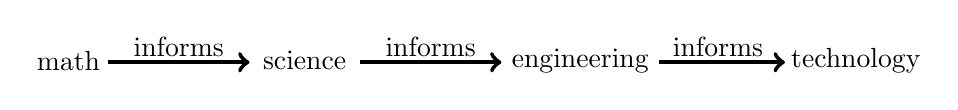
\begin{tikzpicture}
                    \node [align=center] at (0.0, 0.02){math};
                    \draw [ultra thick, ->] (0.5, 0) -- (2.3, 0);
                    \node [align=center] at (1.4, 0.2){informs};
                    \node [align=center] at (3.0, 0.02){science};
                    \draw [ultra thick, ->] (3.7, 0) -- (5.5, 0);
                    \node [align=center] at (4.6, 0.2){informs};
                    \node [align=center] at (6.5, 0.02){engineering};
                    \draw [ultra thick, ->] (7.5, 0) -- (9.1, 0);
                    \node [align=center] at (8.25, 0.2){informs};
                    \node [align=center] at (10, 0.02){technology};
                \end{tikzpicture}
            \end{figure}
                
            However, you'll also find that philosophy informs all of these, and is informed by all of these. The creative arts, like philosophy, is informed by all 4 of these, but tends towards informing only engineering and technology.
                
            This does not mean that mathematics and science is not creative, but it's often misunderstood that because mathematics is so rational, that it's not creative. It takes a lot of creative thinking and intuition, along with rational thought, in order to come up with mathematical proofs, and it is for this reason, and the connections to other fields, that creative arts is a necessary endeavour for anyone learning STEM.
                
            In fact, this is precisely the argument for STEAM.
                
            It must be stated more clearly, because the previous statement may not be clear enough: creative thinking, intuition, and rational thinking are \textbf{all} required for work in each of these fields of study, in concert with each other. Rational thinking does not promote mathematics and science alone. Intuitional thinking will almost certainly lead to falsehoods in these fields, if not matched with rational thinking.
                
            In this sense, creative thinking can be seen to be exploration, finding solution-after-solution, intuitive thinking can be seen to point the creative thinking along, but the rational thinking is the filter that finds the solutions that actually work.
                
            So, you will benefit all of these parts of your mind, including the part of you that is disciplined and builds grit. This will happen by mere practice and use, much like a muscle being used over-and-over getting bigger, and capable of handling more.
                
            Mathematics and the sciences change how you look at the world around you, but it doesn't make you a better person.
        \end{subsection}
        
        \begin{subsection}{The Danger in Strength}
            Philosophy has a long history of beneficial usage and of dangerous misuse. Philosophy may be the most important, but the most dangerous subject matter that a mind can consume. Philosophy has been used to free people as well as enslave people. The philosophical concept of moral or ethical \emph{justification} has been used both to protect and to kill.
            
            In effect, every argument about whether or not human beings are ready for a specific technology is actually a question of whether or not human beings are philosophically mature enough, and is captured in the following quotes:
            
            \begin{quote}{Jason Silva}
                Technology is, of course, a double-edged sword. Fire can cook our food but also burn us.
            \end{quote}
            
            \begin{quote}{Christian Lous Lange}
                Technology is a useful servant, but a dangerous master.
            \end{quote}
            
            \begin{quote}{B. F. Skinner}
                The real problem is not whether machines think, but whether people do.
            \end{quote}
            
            Replace ``technology'' with ``philosophy'' in the first two quotes, and you may begin to understand what it is that I'm claiming. Other quotes are a bit more direct:
            
            \begin{quote}{Martin Luther King, Jr}
                Nothing in all the world is more dangerous than sincere ignorance and conscientious stupidity.
            \end{quote}
            
            \begin{quote}{George Bernard Shaw}
                Beware false knowledge; it is more dangerous than ignorance
            \end{quote}
            
            \begin{quote}{Confucius}
                Real knowledge is to know the extent of one’s ignorance
            \end{quote}
            
            Oftentimes, it is exactly those strengths that serve as one's weaknesses, but that is not to say that having a strength necessarily creates weakness in that area. It benefits us to understand how strengths become weaknesses. 
    
            Philosophy, like technology, is good or bad, depending on how it's used, and depending on how well it's understood, and based on what principles one chooses to work from.
                
            In fact, the call-to-action I give each of you, before you start this endeavour is:
            \begin{itemize}
                \item Use your observations and experiences to help you understand your world
                    
                \item Uproot misperceptions and misunderstandings that come from a partial understanding of the first
                    
                \item Apply your understanding of the world to better your world and the world of others, as you see fit
            \end{itemize}
        \end{subsection}
        
        \begin{samepage}
            \begin{subsection}{Perceptions and Misperceptions of Philosophy, Mathematics, and Science}
                There are multiple misperceptions of about various fields of study, such as:
                \begin{itemize}
                    \item Mathematics
                    \begin{itemize}
                        \item It's not a creative field
                        \item It's the study of numbers
                        \item It's already finished (there's no new math to be had)
                        \item There are no jobs for mathematicians
                    \end{itemize}
                    
                    \item Science
                    \begin{itemize}
                        \item It's done by elite people who have no connection to reality
                        \item It's a collection of statements that are considered ``the truth''
                        \item It doesn't help ``real people''
                    \end{itemize}
                    
                    \item Software Development
                    \begin{itemize}
                        \item It's all copy-and-paste
                        \item Computers will be programming themselves soon
                        \item It's an easy desk-job with little pressure
                    \end{itemize}
                        
                    \item Economics
                    \begin{itemize}
                        \item It's the study of money
                        \item It's all psychology (which contradicts the first claim)
                    \end{itemize}
                \end{itemize}
            \end{subsection}
        \end{samepage}
            
        All of these claims are caricatures of the fields of study, or of the people who do work in those fields, and are not just oversimplifications, but are outright wrong if one were to actually follow these people around.
            
        Much the same misrepresentation occurs in all fields of study and all fields of work. These misrepresentations continue throughout the centuries as populism attempts to change the view of these subjects.
            
        The history of this populism is understood, because in history, fields such as these could only be achieved by the educated and the rich, and those people would not understand those who worked with their hands. Therefore, a schism occurred between those who used their minds, and those who used their hands, based on a classism that is not yet resolved.
            
        A shift has been occurring over the last few centuries though, especially as education has become more universal, allowing people to spend part of their lives in service, part of their lives in manual labor, part of their lives studying, and part of their lives working with their minds, and it's not certain that a person in any particular job has any particular experience.
            
        In this regard, philosophy has always been misrepresented, and you may hear things like:
        \begin{enumerate}
            \item Philosophy, like mathematics, has been completed, or it has produced all of the results and discoveries that it can
                
            \item Philosophy is useless, ungrounded, and a waste of a person's education
                
            \item Philosophy is nebulous, vague, and done by people who are out-of-touch with the real-world
                
            \item Philosophy opposes, is not supported of, or is somehow separate from science
        \end{enumerate}
            
        Nothing could be further from the truth on all of these grounds. Mathematics, and philosophy, are coming up with new discoveries all the time, and including applications to previous discoveries. Philosophy, especially the interest of how we come to know things, forms the basis for both mathematics and the sciences.
    \end{section}
    
    \begin{section}{What is Philosophy, and Why Should We Care?}
        Philosophy is typically introduced by discussing what it means, and where it comes from. We focus so much on the Greek philosophy, but philosophy, mathematics, and science has been growing in all cultures for millennia, and can be found as early trial versions of these subjects in ancient books all over the world.
            
        The word ``philosophy'' is a word from ancient Greek φιλοσοφία (\emph{philosophía}), which has 2 roots:
        \begin{itemize}
            \item φίλος (phílos meaning “loving”)
            \item σοφία (sophía meaning “wisdom”)
        \end{itemize}
            
        However, that only scratches the surface, and tends to lead to the conclusion that “philosophy is in every query”. Although this is technically true, it does little to give anyone any clue to what philosophers actually do, and why it’s important.
            
        In some ways, philosophy is the process of exploring one’s thoughts, asking ourselves, “why do I think this way?”
            
        Specifically, philosophers have certain question that all philosophy branches out from:
            
        \begin{figure}[ht]
            \centering
            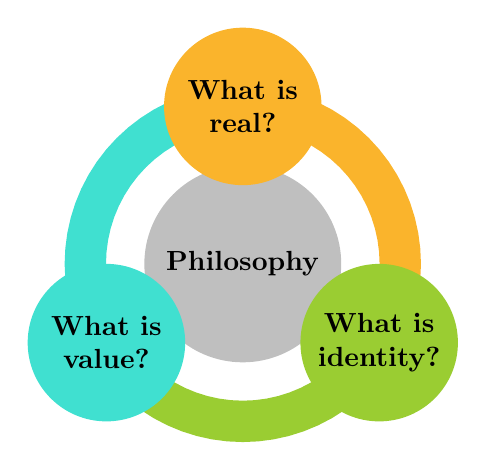
\begin{tikzpicture}
                \fill [lightgray]   (0,0) circle (12.5mm);
                \node [align=center] at (0, 0) {\textbf{Philosophy}};
                \draw [Dandelion,line width=5.25mm,domain=-30:90] plot ({2*cos(\x)},     {2*sin(\x)});
                \draw [YellowGreen,line width=5.25mm,domain=210:330] plot ({2*cos(\x)},     {2*sin(\x)});
                \draw [Turquoise,line width=5.25mm,domain=90:210] plot ({2*cos(\x)},     {2*sin(\x)});
                \fill [Dandelion] (0,2) circle (10mm);
                \fill [YellowGreen] ( 1.732,-1) circle (10mm);
                \fill [Turquoise]   (-1.732,-1) circle (10mm);
                \node [align=center] at ( 0.000, 2) {\textbf{What is}\\\textbf{real?}};
                \node [align=center] at ( 1.732,-1) {\textbf{What is}\\\textbf{identity?}};
                \node [align=center] at (-1.732,-1) {\textbf{What is}\\\textbf{value?}};
            \end{tikzpicture}
            \caption{The 3 Proposed Root Questions of Philosophy.}
            \label{fig:ThreePhilosophicalQuestions}
        \end{figure}
            
        Here though, these 3 questions feed off of each other. For instance, 
        \begin{itemize}
            \item Is it possible to seek truth without asking what methods of truth-seeking that we value?
                
            \item If something exists (if it’s “real” or “true”), can we identify it?
                
            \item If we change something (identity) does it change value?
        \end{itemize}
            
        In fact, these three questions spawn multiple branches of study, some of which are considered philosophical in modern times still, others may appear, on the surface, as if they are something separate from philosophy.
            
        \begin{subsection}{What is Real?}
            Epistemology relates to the question, “How do we know what we know?”. The study     of epistemology has given us logic (forming the foundations of mathematics),     the Scientific Method (forming the foundations of science), and gives us     mechanisms for us to understand beliefs by asking:
                
            \begin{itemize}
                \item What does it mean to know something?
                \item Can anything be known for certain? 
                \item How much confidence can we have in something?
                \item What is the process that we come to know things?
                \item What does it mean to know things?
                \item What is a belief?
                \item Can we justify our beliefs? (\textbf{critical reasoning})
                \item What is the relationship between beliefs and knowledge?     (\textbf{doxastic logic})
            \end{itemize}
        \end{subsection}
            
        \begin{subsection}{What is Identity?}
            In philosophy, we talk about \textbf{discernibility}, which lets us ask, “if two things share all the same properties, are they the same thing?”. We use this in mathematics to present two things being equal. In science, we identify phenomena that interest us. In our lives, we discuss personal identity, social identity, and even discuss the human identity. In many ways, the philosophical focus on definitions and on meanings are directly related to identifying concepts, and coming to agreement on concepts, in order to help discuss.
                
            It leads us to questions like:
                
            \begin{itemize}
                \item What does it mean for two things to be the same, and does that change over time or based on the context?
                \item If I replace every component with an identity component, is it the same thing (Interchangeability and compatibility)?
                \item Are we the same person from one moment to the next?
                \item Is any object the same from one moment to the next?
                \item How do we relate to and do we identify with our city, our culture, and/or our nation?
                \item What does it mean when things are “almost alike” or similar? And do similar things share similar properties?
            \end{itemize}
        \end{subsection}
        \begin{subsection}{What is Value?}
            The notion of \textbf{value} or \textbf{worth} is also of central concern, as it allows us to compare two things. This is also of central concern in mathematics as it allows us to make statements about relationships between things. It is of concern in modern politics, when discussing the value of citizens and whether or not they feel valued. We discuss \textbf{aesthetics} as the study of those things that attract our senses. We discuss \textbf{ethics} through the value of actions. It leads us to questions like:
                
            \begin{itemize}
                \item What does it mean to compare two things?
                \item Why do things cost what they do?
                \item What do individuals value, and why?
                \item What do societies value, and why?
                \item Is something practical worth more than something else? What makes it practical?
                \item What is fairness and justice?
            \end{itemize}
        \end{subsection}
        \begin{subsection}{What is the Relationship Between Value and Identity?}
            When questions about both value and identity come together, we usually start to ask about purpose, and
            \begin{itemize}
                \item Is there a purpose to the existence of the universe? What is the purpose?
                \item Is there a purpose to my existence? What is the purpose? Do I create my own purpose?
                \item Am I a valued part of my community? Why or why not?
                \item What is fair when it comes to treatment of different people?
                \item How does interchangeability relate to comparison? If I interchange components for something newer, is it better?
            \end{itemize}
        \end{subsection}
        \begin{subsection}{What is the Relationship Between Value and Truth?}
            This is the intersection of the two questions that lead us to asking questions like:
            \begin{itemize}
                \item How do we value the various means of obtaining knowledge?
                \item How do people value methods of communicating knowledge and beliefs?
                \item Whose testimonies do we believe and why?
                \item Can there be an absolute, top-level truth, by which all other truths are measured?
                \item Can there be a best moral code, by which all other moral codes are measured?
            \end{itemize}
        \end{subsection}
        \begin{subsection}{What is the Relationship Between Identity and Truth?}
            Regarding identity and truth, we may get some interesting questions about ourselves and:
            \begin{itemize}
                \item What are we? (i.e. what makes us human, or what makes us different?)
                \item Where do we come from?
                \item Why does anything exist at all?
                \item How do we relate to our perceptions, and vice versa?
                \item What does it mean to “exist”?
                \item What does it mean to be “real”?
                \item What is reality?
                \item What is the mind?
            \end{itemize}
        \end{subsection}
        \begin{subsection}{What is the Relationship Between All 3?}
            Finally, we can consider all 3 together:
            \begin{itemize}
                \item Is there something bigger than us?
                \item What is out there, beyond what we can perceive?
                \item How did this universe come to exist? (\textbf{cosmology})
                \item What is the greatest possible mind? Must a creator exist? (\textbf{theology})
            \end{itemize}
        \end{subsection}
            
        \begin{subsection}{Categorizing the Questions into Branches}
            Many of these questions have been placed into various categories:
            \begin{itemize}
                \item That reason can be a source of knowledge (\textbf{rationalism}) allowed us to create logic, and logic continues to refine the foundations of mathematics (classically called, “the formal sciences”)
                    
                \item Critical thinking, using our senses as a source of knowledge (\textbf{empiricism}), building confidence through experimentation (\textbf{verificationism}), and filtering in only those things that we can derive from these sources (\textbf{positivism}) refines the scientific method, which gives us science (classically called, “the physical sciences”)
                
                \item Questions about value form the basis for \textbf{Value Theory}, and include subbranches like: ethics, aesthetics, and axiology (moving into application through economics and politics)
                    
                \item Questions about existence and reality form the basis of \textbf{Metaphysics}, and include subbranches like: theology, religion, and ontology 
                    
                \item Questions about how we do philosophy form the basis of \textbf{Metaphilosophy}
            \end{itemize}
        \end{subsection}
    \end{section}
    
    \begin{section}{Philosophical Discussions}
        So, you thought that this book was going to be about mathematics. Why, then, are we learning philosophy? Well, it turns out that philosophy is the parent of almost every subject studied in any formal education. 
            
        Given that we have asked about reality, science is a formal discipline of the philosophical position called empiricism, allowing us to enter into discussion about those areas of discussion that can be observed and measured with repeatable results. However, as positions go, science is limited to such discussions.
            
        Foremost, we are interested in mathematics in this book, but we will only really get there by discussing the roots of mathematics. Also, in order to understand it, we will do best when we can also link our study to various other areas as well. The most interesting part is how these things link.
            
        \begin{figure}[ht]
            \centering
            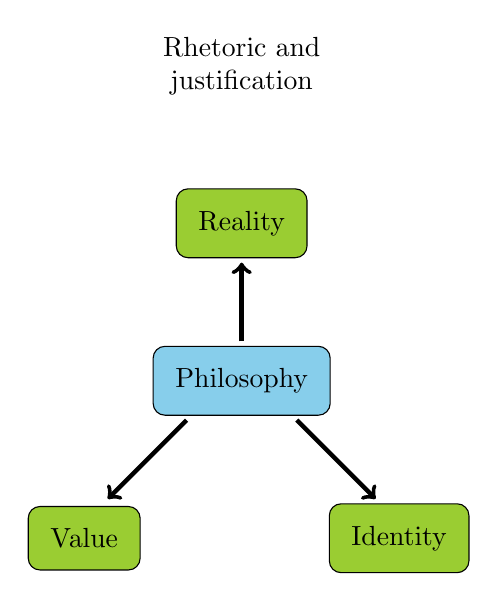
\begin{tikzpicture}
                \node [align=center,draw=black,fill=SkyBlue,thin,inner sep=8pt,rounded corners=.15cm] at (0.0, 0.0) {Philosophy};
                
                \node [align=center,draw=black,fill=YellowGreen,thin,inner sep=8pt,rounded corners=.15cm] at (0.0, 2.0) {Reality};
                
                \node [align=center] at (0.0, 4.0) {Rhetoric and\\justification};
                
                \node [align=center,draw=black,fill=YellowGreen,thin,inner sep=8pt,rounded corners=.15cm] at (-2, -2.0) {Value};
                
                \node [align=center,draw=black,fill=YellowGreen,thin,inner sep=8pt,rounded corners=.15cm] at ( 2, -2.0) {Identity};
                
                \draw [ultra thick, ->] ( 0.0, 0.5) -- (0.0, 1.5);
                \draw [ultra thick, ->] (-0.7,-0.5) -- (-1.7, -1.5);
                \draw [ultra thick, ->] ( 0.7,-0.5) -- ( 1.7, -1.5);
                %\node [align=center] at (0.0, 0.02){math};
                %\draw [ultra thick, ->] (0.5, 0) -- (2.3, 0);
                %\node [align=center] at (1.4, 0.2){informs};
                %\node [align=center] at (3.0, 0.02){science};
                %\draw [ultra thick, ->] (3.7, 0) -- (5.5, 0);
                %\node [align=center] at (4.6, 0.2){informs};
                %\node [align=center] at (6.5, 0.02){engineering};
                %\draw [ultra thick, ->] (7.5, 0) -- (9.1, 0);
                %%\node [align=center] at (8.25, 0.2){informs};
                %\node [align=center] at (10, 0.02){technology};
            \end{tikzpicture}
        \end{figure}
            
        \begin{figure}[H]
            \centering
            \includegraphics[scale=0.65]{PhilosophicalIntroduction/ConnectionsToPhilosophy.png}
            \caption{Connections of Various Fields to Philosophy.}
            \label{fig:ConnectionsToPhilosophy}
        \end{figure}
            
        \begin{subsection}{Rhetoric and Justifying Beliefs}
            It's important to understand that much of our mental sophistication revolves around explaining ourselves to others, whether that be in regards to giving them a mental image of what we have seen, explaining how something works, to justifying our reasons for doing something.
                
            Jonathan Haidt gave us the analogy of our minds being of a human rider on top of an elephant, whereas the rider is the rational mind, and the intuition is the elephant. We are so good at justifying our actions to others, that we often justify things we have done to ourselves, even when we know better (e.g. ``I can eat that whole chocolate cake, because I've done so well on my diet this week.'').
                
            Our written Greek philosophy seems to start with regards to \textbf{rhetoric}, as the ``art of discussion'', developing the communication skills to discuss philosophical positions.
                
            Rhetoric was often divided into:
            \begin{itemize}
                \item \textbf{Emotional} appeals, intended to speak directly to the mind's elephant. These appeals are often highly effective, if sometimes manipulative in their usage.
                    
                \item \textbf{Authoritative} appeals, intended to invoke the authority of the speaker, through their experience or due to their character-history of truthfulness.
                    
                \item \textbf{Rational} appeals, intended to speak directly to the rider of the elephant, who is capable of mapping out a direction for the elephant to travel, if the rider can ever get the elephant to listen.
            \end{itemize}
                
            We may be used to hearing the word rhetoric in political discussions (such as ``inflammatory rhetoric''), but oftentimes the person using the word doesn't mean it with the nuance of the philosophical meaning. Instead, philosophers would deem what politicians are doing \textbf{polemic}, which is emotional arguments intended to reduce confidence in and incite fear of an opponent.
                
            It should be obvious that mathematics and the sciences are filled with logical appeals, and as such, this book will be filled with them as well. However, it's also recognized that the intuition must be brought on board as well. 
                
            Finally, the authoritative appeals should be mostly unused in any discussion of mathematics. There is no for a teacher to use appeals to authority, saying things like ``it just works this way''. The only authoritative appeals will be the usage of already defined and commonly used standards for writing that may be brought up. However, even those should be backed with arguments for rational reasons why.
                
            \begin{subsubsection}{Some Definitions}
                
                \begin{definition}
                    An \textbf{interlocutor} is a person that is taking part in a dialog.
                \end{definition}
                    
                \begin{definition}
                    A \textbf{proposition} is a statement is possibly true or false.
                \end{definition}
                    
                \begin{definition}
                    A \textbf{premise} is a proposition for consideration, sometimes asserted as true by the interlocutor, and sometimes as a condition for the context of the argument.
                \end{definition}
                    
                \begin{definition}
                    A \textbf{conclusion} is a proposition that is the end result that the interlocutor reaches starting from the premises.
                \end{definition}
                    
                \begin{definition}
                    An \textbf{argument} is a series of propositions, structured such that the premises lead to a conclusion. Furthermore, a more general meaning of this word may be a process of reasoning.
                \end{definition}
                    
                \begin{definition}
                    A premise taken as a condition, usually in regards to an investigation is called a \textbf{hypothesis}.
                \end{definition}
                    
                \begin{definition}
                    A \textbf{philosophical position} is a collection of premises that an interlocutor is arguing from.
                        
                    It is often called a \textbf{philosophical theory}, which can cause confusion with the significantly different meanings taken by scientific theory and mathematical theory. 
                        
                    The everyday usage of the word ``theory'' is probably best identified as ``hypothesis''.
                        
                    Due to this confusion, the word position will be preferred in this book.
                \end{definition}
                    
                \begin{figure}[ht]
                    \centering
                    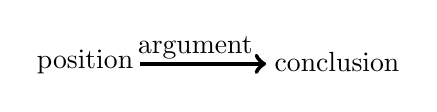
\begin{tikzpicture}
                        \node [align=right] at (0.0, 0.02){position};
                        \draw [ultra thick, ->] (0.7, 0) -- (2.3, 0);
                        \node [align=center] at (1.4, 0.2){argument};
                        \node [align=left] at (3.2, 0.02){conclusion};
                    \end{tikzpicture}
                    \caption{Relation between position (premises), argument, and conclusion}
                \end{figure}
                    
                \begin{definition}
                    For the sake of comparison, a \textbf{life stance} is a philosophical position that one takes, according to their worldview, which informs their beliefs, their thoughts, and their behavior.
                        
                    This is stated separately, since a life stance differs from a philosophical position.
                \end{definition}
                    
                \begin{definition}
                    A \textbf{Devil's Advocate} is a person that argues from a position that differs from their life stance, in order to better understand their own position, and the position of others.
                \end{definition}
                    
                \begin{definition}
                    \textbf{Skepticism} is the act of reserving belief for future evidence.
                \end{definition}
                
                \begin{definition}
                    \textbf{Belief revision} is the act of modifying one or more premises that make up a position, due to new evidence.
                \end{definition}
            \end{subsubsection}
            
            \begin{subsubsection}{What Forms a Worldview}
                At this point, I'm going to present what follows as a position, setting the rest of the book up for discussions on logical reasoning.
                    
                \begin{remark}
                    This position I am starting from, regarding worldviews, is not scientific, is not based on psychological evidence, and is likely just an approximation of how worldviews actually work.
                \end{remark}
                    
                \begin{figure}[ht]
                    \centering
                    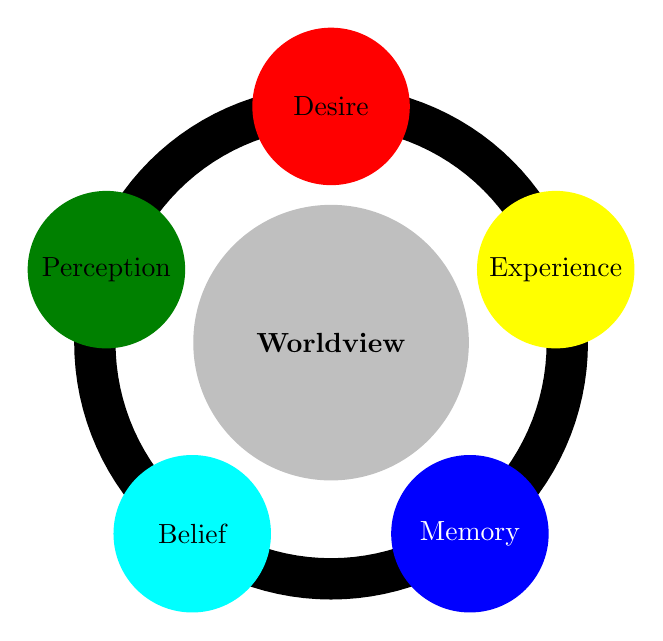
\begin{tikzpicture}
                        \fill [lightgray] (0,0) circle (1.75cm);
                        \node [align=center] at (0, 0) {\textbf{Worldview}};
                            
                        \draw [Black,line width=5.25mm,domain=90:162] plot ({3*cos(\x)}, {3*sin(\x)});
                        \draw [Black,line width=5.25mm,domain=162:234] plot ({3*cos(\x)}, {3*sin(\x)});
                        \draw [Black,line width=5.25mm,domain=234:306] plot ({3*cos(\x)}, {3*sin(\x)});
                        \draw [Black,line width=5.25mm,domain=306:378] plot ({3*cos(\x)}, {3*sin(\x)});
                        \draw [Black,line width=5.25mm,domain=378:450] plot ({3*cos(\x)}, {3*sin(\x)});
                            
                        \fill [Red]   ( 0.000000, 3.000000) circle (10mm);
                        \fill [Green] (-2.853170, 0.927051) circle (10mm);
                        \fill [Cyan]  (-1.763356,-2.427051) circle (10mm);
                        \fill [Blue]  ( 1.763356,-2.427051) circle (10mm);
                        \fill [Yellow]( 2.853170, 0.927051) circle (10mm);
                            
                        \node [align=center,text=black] at 
                        ( 0.000000, 3.000000) {Desire};
                        \node [align=center,text=black] at 
                        (-2.853170, 0.927051) {Perception};
                        \node [align=center,text=black] at 
                        (-1.763356,-2.427051) {Belief};
                        \node [align=center,text=white] at 
                        ( 1.763356,-2.427051) {Memory};
                        \node [align=center,text=black] at 
                        ( 2.853170, 0.927051) {Experience};
                    \end{tikzpicture}
                    \caption{Relation between position (premises), argument, and conclusion}
                \end{figure}
                    
                The first question someone may have looking at the components of a person's worldview that I listed is that experience, memory, and belief are all the same thing. However, my argument is that we experience all the time, but our beliefs color how we interpret the memories associated with those experiences.
                    
                In this sense, we reexperience things through our memory, but it doesn't mean that it feels the same each time.
                    
                It may seem strange that I put desire in with the rest of these, because it appears that the rest of these relate to knowledge, but that desire is completely unrelated. However, we already know that desires change how we perceive things, making us more or less perceptive of our failures or successes, or how other people act.
                    
                The point of all of this is to say that our memories are fallible, because they change. Our perceptions are fallible as well, and so, we cannot always trust our worldview.
            \end{subsubsection}
                
            \begin{subsubsection}{What Sources of Information do you Value?}
                In the discussion of rhetoric, we talked about 3 different types of arguments: emotional, authoritative, and rational.
                    
                However, these are only the methods of transference of information from one person to another, and misses an important source of information: experience.
                    
                We tend to regard experience as the most valued source of information, but as we discussed in regards to the worldview, our perceptions of experiences are often incomplete, and sometimes even wrong.
                    
                Most people, naturally value emotional, authoritative, experiential, intuitive, and rational information sources to some level or another, because we naturally recognize that there are failings with putting all of our trust in any one of them: emotions can sometimes be erratic, people sometimes lie, our perceptions often deceive us, our intuitions are often wrong, and we often don't have enough information to come to a rational conclusion.
                    
                However, there are things that we can do to refine when we use each, and what we can be said about each source of information.
                    
                Firstly, it's important to note that rational arguments begin as intuitive arguments. Humans have an intuitive ability to recognize cause-and-effect, allowing us to determine how things work, and often change how things work to our favor. This recognition of the pattern of cause-and-effect is what leads us to logic, and rational thinking is the disciplined use of this logic. 
                    
                In fact, the discipline is what separates intuition from rational thinking. We follow through with our intuitions to see if they fail.
                    
                Second, the relationship between emotions and intuition are also important. Purely rational thinking is devoid of creativity, can get stuck in analysis, and therefore absent problem solving ability. However, purely intuitive thinking cannot weed out those ideas that won't work, and will naturally try things that are not logically sound, usually wasting their own and other people's time.
                    
                First, let's get more detailed how these each operate as a source of information:
                \begin{itemize}
                        
                    \item Authoritative sources
                    \begin{itemize}
                        \item \textbf{Witnesses} can provide accounts of events
                        \item Parents and teachers often provide us tons of information
                    \end{itemize}
                    \item Experiential sources
                    \begin{itemize}
                        \item Your \textbf{senses} give you access to the world around you and are your connection to it
                        \item When your senses act together they create an \textbf{empirical} view of the world
                        \item This effectively places you as an authority over your own worldview
                        \item Demonstrations from other individuals can help communicate subject matter
                    \end{itemize}
                    \item Emotional and Intuitive sources
                    \begin{itemize}
                        \item Emotions can point us to how our intuitions react to specific experiences
                        \item Gut feelings can tell us things about our world, and are frequently part of our mental pattern-matching capabilities.
                        \item It is via these gut feelings that we are capable of walking, knowing where to place each foot as we move
                        \item The intuitive is unconscious, but quick to form conclusions
                    \end{itemize}
                    \item Rational sources
                    \begin{itemize}
                        \item We use logic and probability to determine whether or not something is possible
                        \item We use analogy to compare and contrast things that we know against things that we do not know
                    \end{itemize}
                \end{itemize}
                    
                We know that authorities can lie, and that witnesses can't always trust their memories. Likewise, we cannot always trust our senses, nor our memories. Our emotions and intuitions are often wrong. Also, we can misuse logic, probability, and analogy.
                    
                In seeking information that we can trust, it seems like we are out of luck, but through careful inspection, we can begin to clear out the mess.
                        
                Regarding rational and intuitive thought, if we learn how to properly use logic and to understand our own biases, we can balance intuition with rational thinking, by allowing intuition to come up with hypotheses, and cutting through the wrong ones via rational thought. We can learn how where rational thinking works, and how sometimes fails us.
                    
                Regarding experience, we can learn about our own psychology, and also through our biases, determine when we can trust our senses and our experiences. We can determine whether multiple memories working together with evidence can corroborate our hypotheses.
                    
                Regarding authorities, \textbf{Subject Matter Experts} are people who are experienced in a subject matter and have a record of insightful discussions, and as long as they have no motive to lie to us, information inside their area of expertise can be trusted.
                    
                From there, we can actually learn what authorities know, how they came to their conclusions, and come to conclusions ourselves via experience and rational thinking.
                    
                So, it's important to think about how and why you value the sources of information that you do, how and why they can fail you, and how to effectively work through them.
            \end{subsubsection}
                
            \begin{subsubsection}{Epistemology}
                The study of what we know and how we come to know it is called \textbf{epistemology}. It is extremely important in the realm of mathematics and the sciences to understand epistemology, 
            \end{subsubsection}
            \begin{subsubsection}{Rigorous Communication}
                Furthermore, most of this communication between experts requires that the words they use are well-understood. We have definitions for words that we use all the time, but often words in a particular \emph{subject matter} have explicit definitions which differ from how they are used in everyday speech.
                    
                Let's consider one of the most problematic words in use today. The word \textbf{theory} from the ancient Greek θεωρία (``theoria'') was contrasted to πρᾶξις (``praxis'' where we get the word ``practice''). The theory behind something was the contemplation regarding how an activity works, and the praxis was the act of doing it. Therefore, theory was used to improve the praxis, but praxis was used to improve the theory.
                    
                This contrasting terminology between the two is why we still have phrases like ``that's works in theory, but not in practice''. However, the meaning of theory in our everyday life is not necessarily how it is used elsewhere:
                    
                \begin{itemize}
                    \item \textbf{Theory (science)} -- a hypothesis which is confirmed by repeated and thorough experimental observation to provide reliable predictions
                    
                    \item \textbf{Theory (mathematics)} -- the collection of premises and conclusions related specific mathematical structures
                        
                    \item \textbf{Theory (philosophy)} -- the collections of premises and conclusions specific to an area of philosophical pursuit (also called a philosophical position).
                        
                    \item \textbf{Theory (everyday speech)} -- a proposed explanation serving as a hypothesis
                \end{itemize}
            \end{subsubsection}
                
                
        \end{subsection}
        \begin{subsection}{Ontology and the Mathematics of Identity, Equality, and Equivalence}
            Discernibility
            Distinguisibility
            Interchangeability
            Identical
                
            \begin{subsubsection}{Definitions}
                In every field of study, we have to be extremely careful what it is we mean when we say something, and aim to avoid
                    
                In mathematics, we often define something, to use in a context (a scope of discussion) and when we are done, we stop meaning it the same. In speech, we do this often with pronouns. For instance, ``Caleb left work. He wasn't feeling that well.''. We immediately know that `He' in the sentence refers to Caleb. In this case, with English, we didn't even specifically define that we'd use `He' this way.
            \end{subsubsection}
                
                
            \begin{subsubsection}{Isomorphisms}
                \begin{definition}
                    The word \textbf{isomorphism} has a formal definition that we will cover later in Category Theory. Philosophically, it can be thought best to first recognize that mathematical objects are conceptual, not physical, and we can argue only that two objects constructed exactly the same way (structural identity) are identical. However, as we have said, two objects can be constructed in 2 different ways and behave as if they are the same object. These objects then have interchangeability between them.
                    
                    An isomorphism focuses, not on identical constructions (what the objects ``are''), but on identical behaviors (what the objects ``do''), and more specifically, that they adhere to the same ``legal contracts'' we call axioms.
                    
                    The word isomorphism (iso- ``same'', -morphism ``form'') is an effective ``equality between types of things''. 
                \end{definition}
                
                An example would be the 2 identical definitions for the number 1:
                \begin{enumerate}
                    \item The natural number comes after 0
                    \item The unique natural number that allows us to multiply any number by itself and result in the same number
                \end{enumerate}
                
                Both of those definitions for 1 focus on what it does, but the first definition is closer to the actual construction of 1 than the second. The two definitions are isomorphic to each other.
                    
                Furthermore, we have the Univalence Axiom, which binds multiple mathematical fields together, in the same way that René Descartés bound algebra together with geometry when he noticed that we can put things on a grid. The proposal of the Univalence Axiom first observed that equivalence (structural identity) implies isomorphism(interchangeability), but the true observation was that an isomorphism was interchangeable with an equivalence.
                
                Now, that's not being fully honest, and yet it is at the same time. A good philosopher will think to themselves, ``you didn't use the word `equivalence' the same way in both of those sentences'', and that philosopher would be right.
                
                I started the discussion talking about identical constructions (what objects ``are''),and obviously, two things cannot be equivalent if they do not have identical constructions. However, equivalence doesn't have to mean identical constructions.Mathematicians often define equivalence based on interchangeability in the same sense as the following analogy:
                
                \begin{quote}
                    A ``Gizmo'' machine has a component called a ``doohickey''. If I can take the doohickey out and replace it with another doohickey, they are interchangeable. If I can replace the Gizmo with another Gizmo, and use the same doohickey in both, then the Gizmo itself is fungible (interchangeable with other things that use components). If any doohickey can go in any Gizmo, then the differences between each doohickey is indiscernible.
                \end{quote}
                
                So, we get an isomorphism between algebraic equations and geometry from Descartés. From Euler we'll see how trigonometry, calculus, and complex numbers relate. However, here we use this opportunity to note that there is an isomorphism between paths, logic,partial orders, computation (and computer science), and tons of things we may get to later, just from Vladimir Voevodsky's Univalence Axiom.
                
                Finally, I have mentioned Axioms as ``legal contracts for mathematical structures''.You may be asking, what structure do we assume Univalence for? We will eventually get into Category Theory, and that will help combine all the world of mathematics together for us.
                
                So, it helps to understand that equality has context, just as isomorphism has context, and we may discuss various types of equalities.
            \end{subsubsection}
                
            \begin{subsubsection}{Natural Numbers are not Non-negative Integers}
                Never does the distinction and non-distinction matter as much as how we teach the number classifications. We have probably been taught that we can identify integers as allowing for negative numbers, and that every natural numbers \textbf{is} an integer.
                    
                This notion of \textbf{is} refers to our isomorphism from earlier. We can construct integers, and we can construct natural numbers, and we will construct them later, but the statement ``\textbf{is}'' used above must be understood to mean that we can get an integer from a natural number, and take that same integer and find a natural number that matches it. That is what it means to ``be the same''.
            \end{subsubsection}
        \end{subsection}
    \end{section}
\end{chapter}
    %\include{Classical Logic}

\documentclass[11pt,twoside,letterpaper,fleqn,parskip=full]{book}

\input{structure}

\makeglossaries
\begin{document}
\newglossaryentry{LawsOfThought}
{
    name={Laws Of Thought},
    description={The 3 laws of classical logic, written down by Aristotle}
}

\newglossaryentry{ClassicalLogic}
{
	name={Classical Logic},
    description={Basic 2-value logic with logical implication, and operations AND, OR, and NOT}
}

\newglossaryentry{BooleanDomain}
{
    name={Boolean Domain},
    description={A domain that has 2 possible-values with the interpretation that one element represents true and the other element represents false}
}
\newglossaryentry{ProofByExhaustion}
{
    name={Proof By Exhaustion},
    description={Creating a deductive proof by analyzing every possible value}
}

\newglossaryentry{bit}
{
    name={bit},
    description={A single element of the Boolean Domain, interpreted as either true or false}
}

\newglossaryentry{symmetry}
{
    name={symmetry},
    description={the property of a relation that allows us to swap the items of the relation}
}

\newglossaryentry{proposition}
{
    name={proposition},
    description={a proposition is statement that can have a truth-value}
}

\newglossaryentry{involution}
{
    name={involution},
    description={Any function that when applied twice produces a result the same as the input}
}

\newglossaryentry{PositionalNotation}
{
    name={Positional Notation},
    description={(also called Place-value notation) uses position to represent numbers, such that numbers that come first have a larger value than those that follow}
}
\nocite{*}
%-- TITLE PAGE --

\begingroup
\thispagestyle{empty}
\centering
\vspace*{5cm}
\par\normalfont\fontsize{35}{35}\sffamily\selectfont
\textbf{Mathematics}\\
{\LARGE Mathematics through Intuition and Rigor}\par % Book title
\vspace*{1cm}
{\Huge Nicholas Cooper}\par % Author name
\endgroup

%-- COPYRIGHT PAGE --

\title{Mathematics}

\newpage
~\vfill
\thispagestyle{empty}

%\noindent Copyright \copyright\ 2014 Andrea Hidalgo\\ % Copyright notice

%\noindent \textsc{github.com/FILLLLLLLLTHISSSSSSSOUTTTTT} % URL

%\noindent This book was created>>>>. % License information

%\noindent \textit{First release, August 2018} % Printing/edition date


%\pagestyle{empty} % No headers

\tableofcontents % Print the table of contents itself

\begin{part}{Graphs, Deduction, and Containers}
    \input{01/Graphs}
    
\end{part}


\begin{part}{Mathematical Introduction to Philosophy and Logic}
    It may seem strange to start off a book of mathematics with philosophy, but I believe that it's necessary, in order to understand what mathematics is, what it's not, and what it's relationship is to other fields of study, such as the sciences. Furthermore, we want to know why we can consider certain things a source of knowledge and why we can trust certain things.
    
    In fact, this ideas fall into the crux of philosophy -- the most important questions, which lead to the remainder of philosophy. This book is not written to necessarily traditional views, and so this discussion of the \emph{roots of philosophy} will be a source of questions that is not typically a focus had by all philosophers.
    
    There are many branches of philosophy, and this book will focus mostly on logic. The book will contain some foundational material for mathematical and scientific inquiry, and the nature of knowledge itself. A brief introductory presentation will be given for philosophical areas of questioning, such as ethics, the nature of being, and the issues that come from poorly understood philosophical positions. Finally, many areas of questioning that philosophy addresses will be absolutely ignored by this book, due to the focus that this book has on mathematical learning.
    
    \begin{chapter}{Introduction to Philosophy}
    No book that mentions philosophy is complete without describing those things that are intended, or valued as goals from the book, or in corporate speak a ``vision'' for the book. This is why this book does not have a formal introduction, but finds an introduction in this section, serving to introduce the importance of formalizing goals when doing work:
        
    \begin{section}{The Intended Value of this Book}
        This is a mathematics book, and the goal of this book is to teach mathematics. However, there are many books which aim to teach mathematics, but the author feels as if there is much missing in the way of:
            
        \begin{itemize}
            \setlength{\itemsep}{6pt}
            \setlength{\parskip}{12pt}
                
            \item \textbf{Intuitions} for the concepts being taught are not commonly taught because our intuitions can often lead us astray. Oftentimes, when we teach analogies, people assume the analogies are more real than analogous, and get angry and upset when the analogies fall apart. Therefore, a long discussion must be had to explain that an analogy doesn't necessarily mean something is equivalent.
     
            \item \textbf{Examples and motivations} of the concepts being used by people. This does not mean that every example needs to be something that is used by everyone, on a daily basis. Mathematics is often argued to be independent from the physical world, and despite the truth in that, the mathematicians who discover these things are not independent of the physical world, and so the physical world still informs the mathematician, and the learner.
               
            \item Because we will focus on examples and motivation from things in the physical world, we will also add \textbf{computer programming} to our learning curriculum, building up to it, nearly from the beginning. This will be a help and a hindrance, because computer literacy and knowledge of how to set up programming environments is not a focus of the lesson plans here. In fact, we should learn what the mathematical concept of a computer is, which is not necessarily the physical thing that this book was written on, but relates to it to a very strong degree.
                
            \item Along the line of the focus on examples, we will collect \textbf{interpretations} of mathematics as it is discussed, and disseminate those interpretations as best possible.
                
            \item Furthermore, the most important thing we will do is to connect various areas of mathematics, so that intuitions from one area will carry over to the other areas, and so will the proofs. Due to this, we may prove some theorems in more than one way in this book, so that the connections can be understood, and to help demonstrate what a theorem really is.
        \end{itemize}
            
        However, the additional focus on the things listed above does not imply that this book can avoid any of the items below, and must be discussed in balance, and with sufficient detail with the following: 
            
        \begin{itemize}
            \setlength{\itemsep}{6pt}
            \setlength{\parskip}{12pt}
                
            \item Formal definitions and descriptions of the concepts, including axiomatic definitions for mathematical structures
                
            \item Various constructions of mathematical structures when possible
                
            \item Formal reasoning for the properties of mathematical structures
        \end{itemize}
            
        You'll notice that these 3 all focus on mathematical structures, which may seem like a foreign concept right now. However, we will provide some heightened understanding of what a mathematical structure is by the end of this book.
            
        The intended reader of this book is adults, and in that respect, it is andragogy (the study of teaching adults), not pedagogy (the study of teaching children). It assumes certain concepts are already understood (like an intuitive feel for the number 250, and of place-value in general); however, it is the author's opinion that the order of subject matter given in this book is approximately the best order to teach children as well, given the mathematical subject matter available as of the year 2020.
    \end{section}
        
    \begin{section}{Motivation to Learn and a Warning to Learn it Well}
        \begin{subsection}{Knowledge is One Source of Strength}
            \begin{quote}{Edward Teller}
                The science of today is the technology of tomorrow.
            \end{quote}
            
            \begin{quote}{Chinese Proverb}
                If your mind is strong, all difficult things will become easy. If your mind is weak, all easy things will become difficult.
            \end{quote}
                
            Since we are still talking about philosophy, another good argument to learn philosophy, and to learn it well, is to build a strong mind through careful analysis of: your values, your own value, what makes you strong, and how you come to understand the world around you.
                
            However, the journey through these analyses are usually very personal. The last one, ``how you come to understand the world around you'' is the only one that this book intends to address in great detail, but being a mathematical book, and not a science book, it's actually less about understanding the physical world, and more about understanding what intuitions are actually happening in your own mind.
                
            We add mathematics to this study, because we realize what it brings to our society, as far as strength goes, by giving us these glimpses into the role that our intuitions have regarding how we interpret the world around us, and how those intuitions sometimes fail, and how often they actually succeed.
                
            The role of mathematics for our society is usually at one end of the chain of information that occurs between the various STEM-based subjects:
                
            \begin{figure}[ht]
                \centering
                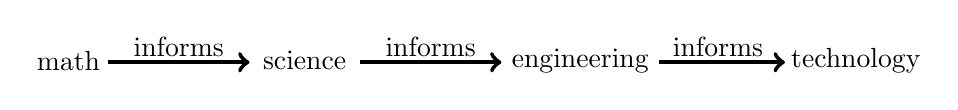
\begin{tikzpicture}
                    \node [align=center] at (0.0, 0.02){math};
                    \draw [ultra thick, ->] (0.5, 0) -- (2.3, 0);
                    \node [align=center] at (1.4, 0.2){informs};
                    \node [align=center] at (3.0, 0.02){science};
                    \draw [ultra thick, ->] (3.7, 0) -- (5.5, 0);
                    \node [align=center] at (4.6, 0.2){informs};
                    \node [align=center] at (6.5, 0.02){engineering};
                    \draw [ultra thick, ->] (7.5, 0) -- (9.1, 0);
                    \node [align=center] at (8.25, 0.2){informs};
                    \node [align=center] at (10, 0.02){technology};
                \end{tikzpicture}
            \end{figure}
                
            However, you'll also find that philosophy informs all of these, and is informed by all of these. The creative arts, like philosophy, is informed by all 4 of these, but tends towards informing only engineering and technology.
                
            This does not mean that mathematics and science is not creative, but it's often misunderstood that because mathematics is so rational, that it's not creative. It takes a lot of creative thinking and intuition, along with rational thought, in order to come up with mathematical proofs, and it is for this reason, and the connections to other fields, that creative arts is a necessary endeavour for anyone learning STEM.
                
            In fact, this is precisely the argument for STEAM.
                
            It must be stated more clearly, because the previous statement may not be clear enough: creative thinking, intuition, and rational thinking are \textbf{all} required for work in each of these fields of study, in concert with each other. Rational thinking does not promote mathematics and science alone. Intuitional thinking will almost certainly lead to falsehoods in these fields, if not matched with rational thinking.
                
            In this sense, creative thinking can be seen to be exploration, finding solution-after-solution, intuitive thinking can be seen to point the creative thinking along, but the rational thinking is the filter that finds the solutions that actually work.
                
            So, you will benefit all of these parts of your mind, including the part of you that is disciplined and builds grit. This will happen by mere practice and use, much like a muscle being used over-and-over getting bigger, and capable of handling more.
                
            Mathematics and the sciences change how you look at the world around you, but it doesn't make you a better person.
        \end{subsection}
        
        \begin{subsection}{The Danger in Strength}
            Philosophy has a long history of beneficial usage and of dangerous misuse. Philosophy may be the most important, but the most dangerous subject matter that a mind can consume. Philosophy has been used to free people as well as enslave people. The philosophical concept of moral or ethical \emph{justification} has been used both to protect and to kill.
            
            In effect, every argument about whether or not human beings are ready for a specific technology is actually a question of whether or not human beings are philosophically mature enough, and is captured in the following quotes:
            
            \begin{quote}{Jason Silva}
                Technology is, of course, a double-edged sword. Fire can cook our food but also burn us.
            \end{quote}
            
            \begin{quote}{Christian Lous Lange}
                Technology is a useful servant, but a dangerous master.
            \end{quote}
            
            \begin{quote}{B. F. Skinner}
                The real problem is not whether machines think, but whether people do.
            \end{quote}
            
            Replace ``technology'' with ``philosophy'' in the first two quotes, and you may begin to understand what it is that I'm claiming. Other quotes are a bit more direct:
            
            \begin{quote}{Martin Luther King, Jr}
                Nothing in all the world is more dangerous than sincere ignorance and conscientious stupidity.
            \end{quote}
            
            \begin{quote}{George Bernard Shaw}
                Beware false knowledge; it is more dangerous than ignorance
            \end{quote}
            
            \begin{quote}{Confucius}
                Real knowledge is to know the extent of one’s ignorance
            \end{quote}
            
            Oftentimes, it is exactly those strengths that serve as one's weaknesses, but that is not to say that having a strength necessarily creates weakness in that area. It benefits us to understand how strengths become weaknesses. 
    
            Philosophy, like technology, is good or bad, depending on how it's used, and depending on how well it's understood, and based on what principles one chooses to work from.
                
            In fact, the call-to-action I give each of you, before you start this endeavour is:
            \begin{itemize}
                \item Use your observations and experiences to help you understand your world
                    
                \item Uproot misperceptions and misunderstandings that come from a partial understanding of the first
                    
                \item Apply your understanding of the world to better your world and the world of others, as you see fit
            \end{itemize}
        \end{subsection}
        
        \begin{samepage}
            \begin{subsection}{Perceptions and Misperceptions of Philosophy, Mathematics, and Science}
                There are multiple misperceptions of about various fields of study, such as:
                \begin{itemize}
                    \item Mathematics
                    \begin{itemize}
                        \item It's not a creative field
                        \item It's the study of numbers
                        \item It's already finished (there's no new math to be had)
                        \item There are no jobs for mathematicians
                    \end{itemize}
                    
                    \item Science
                    \begin{itemize}
                        \item It's done by elite people who have no connection to reality
                        \item It's a collection of statements that are considered ``the truth''
                        \item It doesn't help ``real people''
                    \end{itemize}
                    
                    \item Software Development
                    \begin{itemize}
                        \item It's all copy-and-paste
                        \item Computers will be programming themselves soon
                        \item It's an easy desk-job with little pressure
                    \end{itemize}
                        
                    \item Economics
                    \begin{itemize}
                        \item It's the study of money
                        \item It's all psychology (which contradicts the first claim)
                    \end{itemize}
                \end{itemize}
            \end{subsection}
        \end{samepage}
            
        All of these claims are caricatures of the fields of study, or of the people who do work in those fields, and are not just oversimplifications, but are outright wrong if one were to actually follow these people around.
            
        Much the same misrepresentation occurs in all fields of study and all fields of work. These misrepresentations continue throughout the centuries as populism attempts to change the view of these subjects.
            
        The history of this populism is understood, because in history, fields such as these could only be achieved by the educated and the rich, and those people would not understand those who worked with their hands. Therefore, a schism occurred between those who used their minds, and those who used their hands, based on a classism that is not yet resolved.
            
        A shift has been occurring over the last few centuries though, especially as education has become more universal, allowing people to spend part of their lives in service, part of their lives in manual labor, part of their lives studying, and part of their lives working with their minds, and it's not certain that a person in any particular job has any particular experience.
            
        In this regard, philosophy has always been misrepresented, and you may hear things like:
        \begin{enumerate}
            \item Philosophy, like mathematics, has been completed, or it has produced all of the results and discoveries that it can
                
            \item Philosophy is useless, ungrounded, and a waste of a person's education
                
            \item Philosophy is nebulous, vague, and done by people who are out-of-touch with the real-world
                
            \item Philosophy opposes, is not supported of, or is somehow separate from science
        \end{enumerate}
            
        Nothing could be further from the truth on all of these grounds. Mathematics, and philosophy, are coming up with new discoveries all the time, and including applications to previous discoveries. Philosophy, especially the interest of how we come to know things, forms the basis for both mathematics and the sciences.
    \end{section}
    
    \begin{section}{What is Philosophy, and Why Should We Care?}
        Philosophy is typically introduced by discussing what it means, and where it comes from. We focus so much on the Greek philosophy, but philosophy, mathematics, and science has been growing in all cultures for millennia, and can be found as early trial versions of these subjects in ancient books all over the world.
            
        The word ``philosophy'' is a word from ancient Greek φιλοσοφία (\emph{philosophía}), which has 2 roots:
        \begin{itemize}
            \item φίλος (phílos meaning “loving”)
            \item σοφία (sophía meaning “wisdom”)
        \end{itemize}
            
        However, that only scratches the surface, and tends to lead to the conclusion that “philosophy is in every query”. Although this is technically true, it does little to give anyone any clue to what philosophers actually do, and why it’s important.
            
        In some ways, philosophy is the process of exploring one’s thoughts, asking ourselves, “why do I think this way?”
            
        Specifically, philosophers have certain question that all philosophy branches out from:
            
        \begin{figure}[ht]
            \centering
            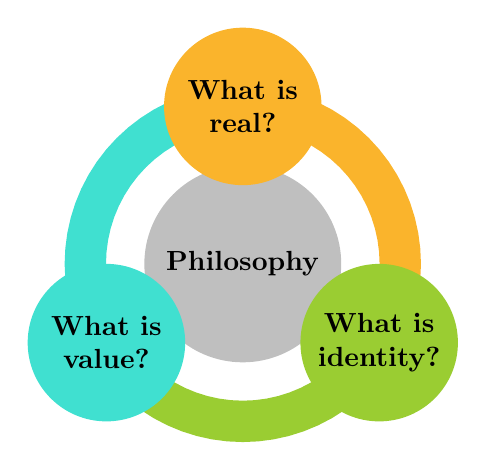
\begin{tikzpicture}
                \fill [lightgray]   (0,0) circle (12.5mm);
                \node [align=center] at (0, 0) {\textbf{Philosophy}};
                \draw [Dandelion,line width=5.25mm,domain=-30:90] plot ({2*cos(\x)},     {2*sin(\x)});
                \draw [YellowGreen,line width=5.25mm,domain=210:330] plot ({2*cos(\x)},     {2*sin(\x)});
                \draw [Turquoise,line width=5.25mm,domain=90:210] plot ({2*cos(\x)},     {2*sin(\x)});
                \fill [Dandelion] (0,2) circle (10mm);
                \fill [YellowGreen] ( 1.732,-1) circle (10mm);
                \fill [Turquoise]   (-1.732,-1) circle (10mm);
                \node [align=center] at ( 0.000, 2) {\textbf{What is}\\\textbf{real?}};
                \node [align=center] at ( 1.732,-1) {\textbf{What is}\\\textbf{identity?}};
                \node [align=center] at (-1.732,-1) {\textbf{What is}\\\textbf{value?}};
            \end{tikzpicture}
            \caption{The 3 Proposed Root Questions of Philosophy.}
            \label{fig:ThreePhilosophicalQuestions}
        \end{figure}
            
        Here though, these 3 questions feed off of each other. For instance, 
        \begin{itemize}
            \item Is it possible to seek truth without asking what methods of truth-seeking that we value?
                
            \item If something exists (if it’s “real” or “true”), can we identify it?
                
            \item If we change something (identity) does it change value?
        \end{itemize}
            
        In fact, these three questions spawn multiple branches of study, some of which are considered philosophical in modern times still, others may appear, on the surface, as if they are something separate from philosophy.
            
        \begin{subsection}{What is Real?}
            Epistemology relates to the question, “How do we know what we know?”. The study     of epistemology has given us logic (forming the foundations of mathematics),     the Scientific Method (forming the foundations of science), and gives us     mechanisms for us to understand beliefs by asking:
                
            \begin{itemize}
                \item What does it mean to know something?
                \item Can anything be known for certain? 
                \item How much confidence can we have in something?
                \item What is the process that we come to know things?
                \item What does it mean to know things?
                \item What is a belief?
                \item Can we justify our beliefs? (\textbf{critical reasoning})
                \item What is the relationship between beliefs and knowledge?     (\textbf{doxastic logic})
            \end{itemize}
        \end{subsection}
            
        \begin{subsection}{What is Identity?}
            In philosophy, we talk about \textbf{discernibility}, which lets us ask, “if two things share all the same properties, are they the same thing?”. We use this in mathematics to present two things being equal. In science, we identify phenomena that interest us. In our lives, we discuss personal identity, social identity, and even discuss the human identity. In many ways, the philosophical focus on definitions and on meanings are directly related to identifying concepts, and coming to agreement on concepts, in order to help discuss.
                
            It leads us to questions like:
                
            \begin{itemize}
                \item What does it mean for two things to be the same, and does that change over time or based on the context?
                \item If I replace every component with an identity component, is it the same thing (Interchangeability and compatibility)?
                \item Are we the same person from one moment to the next?
                \item Is any object the same from one moment to the next?
                \item How do we relate to and do we identify with our city, our culture, and/or our nation?
                \item What does it mean when things are “almost alike” or similar? And do similar things share similar properties?
            \end{itemize}
        \end{subsection}
        \begin{subsection}{What is Value?}
            The notion of \textbf{value} or \textbf{worth} is also of central concern, as it allows us to compare two things. This is also of central concern in mathematics as it allows us to make statements about relationships between things. It is of concern in modern politics, when discussing the value of citizens and whether or not they feel valued. We discuss \textbf{aesthetics} as the study of those things that attract our senses. We discuss \textbf{ethics} through the value of actions. It leads us to questions like:
                
            \begin{itemize}
                \item What does it mean to compare two things?
                \item Why do things cost what they do?
                \item What do individuals value, and why?
                \item What do societies value, and why?
                \item Is something practical worth more than something else? What makes it practical?
                \item What is fairness and justice?
            \end{itemize}
        \end{subsection}
        \begin{subsection}{What is the Relationship Between Value and Identity?}
            When questions about both value and identity come together, we usually start to ask about purpose, and
            \begin{itemize}
                \item Is there a purpose to the existence of the universe? What is the purpose?
                \item Is there a purpose to my existence? What is the purpose? Do I create my own purpose?
                \item Am I a valued part of my community? Why or why not?
                \item What is fair when it comes to treatment of different people?
                \item How does interchangeability relate to comparison? If I interchange components for something newer, is it better?
            \end{itemize}
        \end{subsection}
        \begin{subsection}{What is the Relationship Between Value and Truth?}
            This is the intersection of the two questions that lead us to asking questions like:
            \begin{itemize}
                \item How do we value the various means of obtaining knowledge?
                \item How do people value methods of communicating knowledge and beliefs?
                \item Whose testimonies do we believe and why?
                \item Can there be an absolute, top-level truth, by which all other truths are measured?
                \item Can there be a best moral code, by which all other moral codes are measured?
            \end{itemize}
        \end{subsection}
        \begin{subsection}{What is the Relationship Between Identity and Truth?}
            Regarding identity and truth, we may get some interesting questions about ourselves and:
            \begin{itemize}
                \item What are we? (i.e. what makes us human, or what makes us different?)
                \item Where do we come from?
                \item Why does anything exist at all?
                \item How do we relate to our perceptions, and vice versa?
                \item What does it mean to “exist”?
                \item What does it mean to be “real”?
                \item What is reality?
                \item What is the mind?
            \end{itemize}
        \end{subsection}
        \begin{subsection}{What is the Relationship Between All 3?}
            Finally, we can consider all 3 together:
            \begin{itemize}
                \item Is there something bigger than us?
                \item What is out there, beyond what we can perceive?
                \item How did this universe come to exist? (\textbf{cosmology})
                \item What is the greatest possible mind? Must a creator exist? (\textbf{theology})
            \end{itemize}
        \end{subsection}
            
        \begin{subsection}{Categorizing the Questions into Branches}
            Many of these questions have been placed into various categories:
            \begin{itemize}
                \item That reason can be a source of knowledge (\textbf{rationalism}) allowed us to create logic, and logic continues to refine the foundations of mathematics (classically called, “the formal sciences”)
                    
                \item Critical thinking, using our senses as a source of knowledge (\textbf{empiricism}), building confidence through experimentation (\textbf{verificationism}), and filtering in only those things that we can derive from these sources (\textbf{positivism}) refines the scientific method, which gives us science (classically called, “the physical sciences”)
                
                \item Questions about value form the basis for \textbf{Value Theory}, and include subbranches like: ethics, aesthetics, and axiology (moving into application through economics and politics)
                    
                \item Questions about existence and reality form the basis of \textbf{Metaphysics}, and include subbranches like: theology, religion, and ontology 
                    
                \item Questions about how we do philosophy form the basis of \textbf{Metaphilosophy}
            \end{itemize}
        \end{subsection}
    \end{section}
    
    \begin{section}{Philosophical Discussions}
        So, you thought that this book was going to be about mathematics. Why, then, are we learning philosophy? Well, it turns out that philosophy is the parent of almost every subject studied in any formal education. 
            
        Given that we have asked about reality, science is a formal discipline of the philosophical position called empiricism, allowing us to enter into discussion about those areas of discussion that can be observed and measured with repeatable results. However, as positions go, science is limited to such discussions.
            
        Foremost, we are interested in mathematics in this book, but we will only really get there by discussing the roots of mathematics. Also, in order to understand it, we will do best when we can also link our study to various other areas as well. The most interesting part is how these things link.
            
        \begin{figure}[ht]
            \centering
            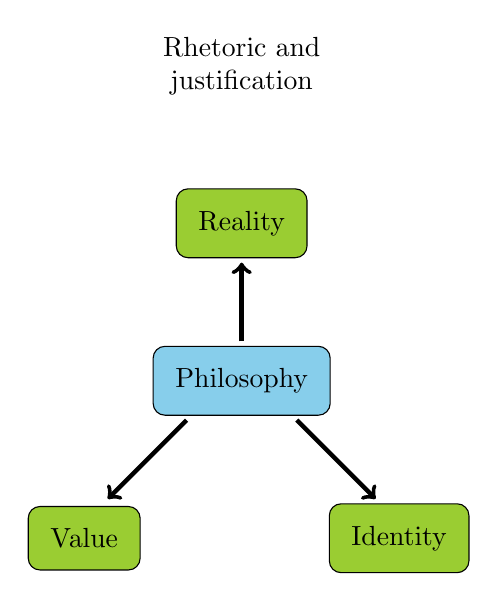
\begin{tikzpicture}
                \node [align=center,draw=black,fill=SkyBlue,thin,inner sep=8pt,rounded corners=.15cm] at (0.0, 0.0) {Philosophy};
                
                \node [align=center,draw=black,fill=YellowGreen,thin,inner sep=8pt,rounded corners=.15cm] at (0.0, 2.0) {Reality};
                
                \node [align=center] at (0.0, 4.0) {Rhetoric and\\justification};
                
                \node [align=center,draw=black,fill=YellowGreen,thin,inner sep=8pt,rounded corners=.15cm] at (-2, -2.0) {Value};
                
                \node [align=center,draw=black,fill=YellowGreen,thin,inner sep=8pt,rounded corners=.15cm] at ( 2, -2.0) {Identity};
                
                \draw [ultra thick, ->] ( 0.0, 0.5) -- (0.0, 1.5);
                \draw [ultra thick, ->] (-0.7,-0.5) -- (-1.7, -1.5);
                \draw [ultra thick, ->] ( 0.7,-0.5) -- ( 1.7, -1.5);
                %\node [align=center] at (0.0, 0.02){math};
                %\draw [ultra thick, ->] (0.5, 0) -- (2.3, 0);
                %\node [align=center] at (1.4, 0.2){informs};
                %\node [align=center] at (3.0, 0.02){science};
                %\draw [ultra thick, ->] (3.7, 0) -- (5.5, 0);
                %\node [align=center] at (4.6, 0.2){informs};
                %\node [align=center] at (6.5, 0.02){engineering};
                %\draw [ultra thick, ->] (7.5, 0) -- (9.1, 0);
                %%\node [align=center] at (8.25, 0.2){informs};
                %\node [align=center] at (10, 0.02){technology};
            \end{tikzpicture}
        \end{figure}
            
        \begin{figure}[H]
            \centering
            \includegraphics[scale=0.65]{PhilosophicalIntroduction/ConnectionsToPhilosophy.png}
            \caption{Connections of Various Fields to Philosophy.}
            \label{fig:ConnectionsToPhilosophy}
        \end{figure}
            
        \begin{subsection}{Rhetoric and Justifying Beliefs}
            It's important to understand that much of our mental sophistication revolves around explaining ourselves to others, whether that be in regards to giving them a mental image of what we have seen, explaining how something works, to justifying our reasons for doing something.
                
            Jonathan Haidt gave us the analogy of our minds being of a human rider on top of an elephant, whereas the rider is the rational mind, and the intuition is the elephant. We are so good at justifying our actions to others, that we often justify things we have done to ourselves, even when we know better (e.g. ``I can eat that whole chocolate cake, because I've done so well on my diet this week.'').
                
            Our written Greek philosophy seems to start with regards to \textbf{rhetoric}, as the ``art of discussion'', developing the communication skills to discuss philosophical positions.
                
            Rhetoric was often divided into:
            \begin{itemize}
                \item \textbf{Emotional} appeals, intended to speak directly to the mind's elephant. These appeals are often highly effective, if sometimes manipulative in their usage.
                    
                \item \textbf{Authoritative} appeals, intended to invoke the authority of the speaker, through their experience or due to their character-history of truthfulness.
                    
                \item \textbf{Rational} appeals, intended to speak directly to the rider of the elephant, who is capable of mapping out a direction for the elephant to travel, if the rider can ever get the elephant to listen.
            \end{itemize}
                
            We may be used to hearing the word rhetoric in political discussions (such as ``inflammatory rhetoric''), but oftentimes the person using the word doesn't mean it with the nuance of the philosophical meaning. Instead, philosophers would deem what politicians are doing \textbf{polemic}, which is emotional arguments intended to reduce confidence in and incite fear of an opponent.
                
            It should be obvious that mathematics and the sciences are filled with logical appeals, and as such, this book will be filled with them as well. However, it's also recognized that the intuition must be brought on board as well. 
                
            Finally, the authoritative appeals should be mostly unused in any discussion of mathematics. There is no for a teacher to use appeals to authority, saying things like ``it just works this way''. The only authoritative appeals will be the usage of already defined and commonly used standards for writing that may be brought up. However, even those should be backed with arguments for rational reasons why.
                
            \begin{subsubsection}{Some Definitions}
                
                \begin{definition}
                    An \textbf{interlocutor} is a person that is taking part in a dialog.
                \end{definition}
                    
                \begin{definition}
                    A \textbf{proposition} is a statement is possibly true or false.
                \end{definition}
                    
                \begin{definition}
                    A \textbf{premise} is a proposition for consideration, sometimes asserted as true by the interlocutor, and sometimes as a condition for the context of the argument.
                \end{definition}
                    
                \begin{definition}
                    A \textbf{conclusion} is a proposition that is the end result that the interlocutor reaches starting from the premises.
                \end{definition}
                    
                \begin{definition}
                    An \textbf{argument} is a series of propositions, structured such that the premises lead to a conclusion. Furthermore, a more general meaning of this word may be a process of reasoning.
                \end{definition}
                    
                \begin{definition}
                    A premise taken as a condition, usually in regards to an investigation is called a \textbf{hypothesis}.
                \end{definition}
                    
                \begin{definition}
                    A \textbf{philosophical position} is a collection of premises that an interlocutor is arguing from.
                        
                    It is often called a \textbf{philosophical theory}, which can cause confusion with the significantly different meanings taken by scientific theory and mathematical theory. 
                        
                    The everyday usage of the word ``theory'' is probably best identified as ``hypothesis''.
                        
                    Due to this confusion, the word position will be preferred in this book.
                \end{definition}
                    
                \begin{figure}[ht]
                    \centering
                    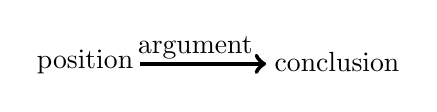
\begin{tikzpicture}
                        \node [align=right] at (0.0, 0.02){position};
                        \draw [ultra thick, ->] (0.7, 0) -- (2.3, 0);
                        \node [align=center] at (1.4, 0.2){argument};
                        \node [align=left] at (3.2, 0.02){conclusion};
                    \end{tikzpicture}
                    \caption{Relation between position (premises), argument, and conclusion}
                \end{figure}
                    
                \begin{definition}
                    For the sake of comparison, a \textbf{life stance} is a philosophical position that one takes, according to their worldview, which informs their beliefs, their thoughts, and their behavior.
                        
                    This is stated separately, since a life stance differs from a philosophical position.
                \end{definition}
                    
                \begin{definition}
                    A \textbf{Devil's Advocate} is a person that argues from a position that differs from their life stance, in order to better understand their own position, and the position of others.
                \end{definition}
                    
                \begin{definition}
                    \textbf{Skepticism} is the act of reserving belief for future evidence.
                \end{definition}
                
                \begin{definition}
                    \textbf{Belief revision} is the act of modifying one or more premises that make up a position, due to new evidence.
                \end{definition}
            \end{subsubsection}
            
            \begin{subsubsection}{What Forms a Worldview}
                At this point, I'm going to present what follows as a position, setting the rest of the book up for discussions on logical reasoning.
                    
                \begin{remark}
                    This position I am starting from, regarding worldviews, is not scientific, is not based on psychological evidence, and is likely just an approximation of how worldviews actually work.
                \end{remark}
                    
                \begin{figure}[ht]
                    \centering
                    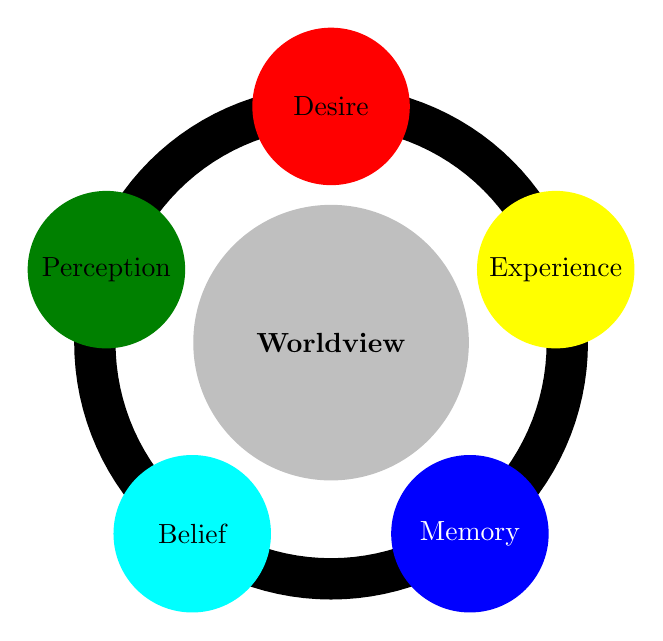
\begin{tikzpicture}
                        \fill [lightgray] (0,0) circle (1.75cm);
                        \node [align=center] at (0, 0) {\textbf{Worldview}};
                            
                        \draw [Black,line width=5.25mm,domain=90:162] plot ({3*cos(\x)}, {3*sin(\x)});
                        \draw [Black,line width=5.25mm,domain=162:234] plot ({3*cos(\x)}, {3*sin(\x)});
                        \draw [Black,line width=5.25mm,domain=234:306] plot ({3*cos(\x)}, {3*sin(\x)});
                        \draw [Black,line width=5.25mm,domain=306:378] plot ({3*cos(\x)}, {3*sin(\x)});
                        \draw [Black,line width=5.25mm,domain=378:450] plot ({3*cos(\x)}, {3*sin(\x)});
                            
                        \fill [Red]   ( 0.000000, 3.000000) circle (10mm);
                        \fill [Green] (-2.853170, 0.927051) circle (10mm);
                        \fill [Cyan]  (-1.763356,-2.427051) circle (10mm);
                        \fill [Blue]  ( 1.763356,-2.427051) circle (10mm);
                        \fill [Yellow]( 2.853170, 0.927051) circle (10mm);
                            
                        \node [align=center,text=black] at 
                        ( 0.000000, 3.000000) {Desire};
                        \node [align=center,text=black] at 
                        (-2.853170, 0.927051) {Perception};
                        \node [align=center,text=black] at 
                        (-1.763356,-2.427051) {Belief};
                        \node [align=center,text=white] at 
                        ( 1.763356,-2.427051) {Memory};
                        \node [align=center,text=black] at 
                        ( 2.853170, 0.927051) {Experience};
                    \end{tikzpicture}
                    \caption{Relation between position (premises), argument, and conclusion}
                \end{figure}
                    
                The first question someone may have looking at the components of a person's worldview that I listed is that experience, memory, and belief are all the same thing. However, my argument is that we experience all the time, but our beliefs color how we interpret the memories associated with those experiences.
                    
                In this sense, we reexperience things through our memory, but it doesn't mean that it feels the same each time.
                    
                It may seem strange that I put desire in with the rest of these, because it appears that the rest of these relate to knowledge, but that desire is completely unrelated. However, we already know that desires change how we perceive things, making us more or less perceptive of our failures or successes, or how other people act.
                    
                The point of all of this is to say that our memories are fallible, because they change. Our perceptions are fallible as well, and so, we cannot always trust our worldview.
            \end{subsubsection}
                
            \begin{subsubsection}{What Sources of Information do you Value?}
                In the discussion of rhetoric, we talked about 3 different types of arguments: emotional, authoritative, and rational.
                    
                However, these are only the methods of transference of information from one person to another, and misses an important source of information: experience.
                    
                We tend to regard experience as the most valued source of information, but as we discussed in regards to the worldview, our perceptions of experiences are often incomplete, and sometimes even wrong.
                    
                Most people, naturally value emotional, authoritative, experiential, intuitive, and rational information sources to some level or another, because we naturally recognize that there are failings with putting all of our trust in any one of them: emotions can sometimes be erratic, people sometimes lie, our perceptions often deceive us, our intuitions are often wrong, and we often don't have enough information to come to a rational conclusion.
                    
                However, there are things that we can do to refine when we use each, and what we can be said about each source of information.
                    
                Firstly, it's important to note that rational arguments begin as intuitive arguments. Humans have an intuitive ability to recognize cause-and-effect, allowing us to determine how things work, and often change how things work to our favor. This recognition of the pattern of cause-and-effect is what leads us to logic, and rational thinking is the disciplined use of this logic. 
                    
                In fact, the discipline is what separates intuition from rational thinking. We follow through with our intuitions to see if they fail.
                    
                Second, the relationship between emotions and intuition are also important. Purely rational thinking is devoid of creativity, can get stuck in analysis, and therefore absent problem solving ability. However, purely intuitive thinking cannot weed out those ideas that won't work, and will naturally try things that are not logically sound, usually wasting their own and other people's time.
                    
                First, let's get more detailed how these each operate as a source of information:
                \begin{itemize}
                        
                    \item Authoritative sources
                    \begin{itemize}
                        \item \textbf{Witnesses} can provide accounts of events
                        \item Parents and teachers often provide us tons of information
                    \end{itemize}
                    \item Experiential sources
                    \begin{itemize}
                        \item Your \textbf{senses} give you access to the world around you and are your connection to it
                        \item When your senses act together they create an \textbf{empirical} view of the world
                        \item This effectively places you as an authority over your own worldview
                        \item Demonstrations from other individuals can help communicate subject matter
                    \end{itemize}
                    \item Emotional and Intuitive sources
                    \begin{itemize}
                        \item Emotions can point us to how our intuitions react to specific experiences
                        \item Gut feelings can tell us things about our world, and are frequently part of our mental pattern-matching capabilities.
                        \item It is via these gut feelings that we are capable of walking, knowing where to place each foot as we move
                        \item The intuitive is unconscious, but quick to form conclusions
                    \end{itemize}
                    \item Rational sources
                    \begin{itemize}
                        \item We use logic and probability to determine whether or not something is possible
                        \item We use analogy to compare and contrast things that we know against things that we do not know
                    \end{itemize}
                \end{itemize}
                    
                We know that authorities can lie, and that witnesses can't always trust their memories. Likewise, we cannot always trust our senses, nor our memories. Our emotions and intuitions are often wrong. Also, we can misuse logic, probability, and analogy.
                    
                In seeking information that we can trust, it seems like we are out of luck, but through careful inspection, we can begin to clear out the mess.
                        
                Regarding rational and intuitive thought, if we learn how to properly use logic and to understand our own biases, we can balance intuition with rational thinking, by allowing intuition to come up with hypotheses, and cutting through the wrong ones via rational thought. We can learn how where rational thinking works, and how sometimes fails us.
                    
                Regarding experience, we can learn about our own psychology, and also through our biases, determine when we can trust our senses and our experiences. We can determine whether multiple memories working together with evidence can corroborate our hypotheses.
                    
                Regarding authorities, \textbf{Subject Matter Experts} are people who are experienced in a subject matter and have a record of insightful discussions, and as long as they have no motive to lie to us, information inside their area of expertise can be trusted.
                    
                From there, we can actually learn what authorities know, how they came to their conclusions, and come to conclusions ourselves via experience and rational thinking.
                    
                So, it's important to think about how and why you value the sources of information that you do, how and why they can fail you, and how to effectively work through them.
            \end{subsubsection}
                
            \begin{subsubsection}{Epistemology}
                The study of what we know and how we come to know it is called \textbf{epistemology}. It is extremely important in the realm of mathematics and the sciences to understand epistemology, 
            \end{subsubsection}
            \begin{subsubsection}{Rigorous Communication}
                Furthermore, most of this communication between experts requires that the words they use are well-understood. We have definitions for words that we use all the time, but often words in a particular \emph{subject matter} have explicit definitions which differ from how they are used in everyday speech.
                    
                Let's consider one of the most problematic words in use today. The word \textbf{theory} from the ancient Greek θεωρία (``theoria'') was contrasted to πρᾶξις (``praxis'' where we get the word ``practice''). The theory behind something was the contemplation regarding how an activity works, and the praxis was the act of doing it. Therefore, theory was used to improve the praxis, but praxis was used to improve the theory.
                    
                This contrasting terminology between the two is why we still have phrases like ``that's works in theory, but not in practice''. However, the meaning of theory in our everyday life is not necessarily how it is used elsewhere:
                    
                \begin{itemize}
                    \item \textbf{Theory (science)} -- a hypothesis which is confirmed by repeated and thorough experimental observation to provide reliable predictions
                    
                    \item \textbf{Theory (mathematics)} -- the collection of premises and conclusions related specific mathematical structures
                        
                    \item \textbf{Theory (philosophy)} -- the collections of premises and conclusions specific to an area of philosophical pursuit (also called a philosophical position).
                        
                    \item \textbf{Theory (everyday speech)} -- a proposed explanation serving as a hypothesis
                \end{itemize}
            \end{subsubsection}
                
                
        \end{subsection}
        \begin{subsection}{Ontology and the Mathematics of Identity, Equality, and Equivalence}
            Discernibility
            Distinguisibility
            Interchangeability
            Identical
                
            \begin{subsubsection}{Definitions}
                In every field of study, we have to be extremely careful what it is we mean when we say something, and aim to avoid
                    
                In mathematics, we often define something, to use in a context (a scope of discussion) and when we are done, we stop meaning it the same. In speech, we do this often with pronouns. For instance, ``Caleb left work. He wasn't feeling that well.''. We immediately know that `He' in the sentence refers to Caleb. In this case, with English, we didn't even specifically define that we'd use `He' this way.
            \end{subsubsection}
                
                
            \begin{subsubsection}{Isomorphisms}
                \begin{definition}
                    The word \textbf{isomorphism} has a formal definition that we will cover later in Category Theory. Philosophically, it can be thought best to first recognize that mathematical objects are conceptual, not physical, and we can argue only that two objects constructed exactly the same way (structural identity) are identical. However, as we have said, two objects can be constructed in 2 different ways and behave as if they are the same object. These objects then have interchangeability between them.
                    
                    An isomorphism focuses, not on identical constructions (what the objects ``are''), but on identical behaviors (what the objects ``do''), and more specifically, that they adhere to the same ``legal contracts'' we call axioms.
                    
                    The word isomorphism (iso- ``same'', -morphism ``form'') is an effective ``equality between types of things''. 
                \end{definition}
                
                An example would be the 2 identical definitions for the number 1:
                \begin{enumerate}
                    \item The natural number comes after 0
                    \item The unique natural number that allows us to multiply any number by itself and result in the same number
                \end{enumerate}
                
                Both of those definitions for 1 focus on what it does, but the first definition is closer to the actual construction of 1 than the second. The two definitions are isomorphic to each other.
                    
                Furthermore, we have the Univalence Axiom, which binds multiple mathematical fields together, in the same way that René Descartés bound algebra together with geometry when he noticed that we can put things on a grid. The proposal of the Univalence Axiom first observed that equivalence (structural identity) implies isomorphism(interchangeability), but the true observation was that an isomorphism was interchangeable with an equivalence.
                
                Now, that's not being fully honest, and yet it is at the same time. A good philosopher will think to themselves, ``you didn't use the word `equivalence' the same way in both of those sentences'', and that philosopher would be right.
                
                I started the discussion talking about identical constructions (what objects ``are''),and obviously, two things cannot be equivalent if they do not have identical constructions. However, equivalence doesn't have to mean identical constructions.Mathematicians often define equivalence based on interchangeability in the same sense as the following analogy:
                
                \begin{quote}
                    A ``Gizmo'' machine has a component called a ``doohickey''. If I can take the doohickey out and replace it with another doohickey, they are interchangeable. If I can replace the Gizmo with another Gizmo, and use the same doohickey in both, then the Gizmo itself is fungible (interchangeable with other things that use components). If any doohickey can go in any Gizmo, then the differences between each doohickey is indiscernible.
                \end{quote}
                
                So, we get an isomorphism between algebraic equations and geometry from Descartés. From Euler we'll see how trigonometry, calculus, and complex numbers relate. However, here we use this opportunity to note that there is an isomorphism between paths, logic,partial orders, computation (and computer science), and tons of things we may get to later, just from Vladimir Voevodsky's Univalence Axiom.
                
                Finally, I have mentioned Axioms as ``legal contracts for mathematical structures''.You may be asking, what structure do we assume Univalence for? We will eventually get into Category Theory, and that will help combine all the world of mathematics together for us.
                
                So, it helps to understand that equality has context, just as isomorphism has context, and we may discuss various types of equalities.
            \end{subsubsection}
                
            \begin{subsubsection}{Natural Numbers are not Non-negative Integers}
                Never does the distinction and non-distinction matter as much as how we teach the number classifications. We have probably been taught that we can identify integers as allowing for negative numbers, and that every natural numbers \textbf{is} an integer.
                    
                This notion of \textbf{is} refers to our isomorphism from earlier. We can construct integers, and we can construct natural numbers, and we will construct them later, but the statement ``\textbf{is}'' used above must be understood to mean that we can get an integer from a natural number, and take that same integer and find a natural number that matches it. That is what it means to ``be the same''.
            \end{subsubsection}
        \end{subsection}
    \end{section}
\end{chapter}
    %\include{Classical Logic}

\documentclass[11pt,twoside,letterpaper,fleqn,parskip=full]{book}

\input{structure}

\makeglossaries
\begin{document}
\input{glossary.tex}
\nocite{*}
%-- TITLE PAGE --

\begingroup
\thispagestyle{empty}
\centering
\vspace*{5cm}
\par\normalfont\fontsize{35}{35}\sffamily\selectfont
\textbf{Mathematics}\\
{\LARGE Mathematics through Intuition and Rigor}\par % Book title
\vspace*{1cm}
{\Huge Nicholas Cooper}\par % Author name
\endgroup

%-- COPYRIGHT PAGE --

\title{Mathematics}

\newpage
~\vfill
\thispagestyle{empty}

%\noindent Copyright \copyright\ 2014 Andrea Hidalgo\\ % Copyright notice

%\noindent \textsc{github.com/FILLLLLLLLTHISSSSSSSOUTTTTT} % URL

%\noindent This book was created>>>>. % License information

%\noindent \textit{First release, August 2018} % Printing/edition date


%\pagestyle{empty} % No headers

\tableofcontents % Print the table of contents itself

\include{01/main}


\begin{part}{Mathematical Introduction to Philosophy and Logic}
    It may seem strange to start off a book of mathematics with philosophy, but I believe that it's necessary, in order to understand what mathematics is, what it's not, and what it's relationship is to other fields of study, such as the sciences. Furthermore, we want to know why we can consider certain things a source of knowledge and why we can trust certain things.
    
    In fact, this ideas fall into the crux of philosophy -- the most important questions, which lead to the remainder of philosophy. This book is not written to necessarily traditional views, and so this discussion of the \emph{roots of philosophy} will be a source of questions that is not typically a focus had by all philosophers.
    
    There are many branches of philosophy, and this book will focus mostly on logic. The book will contain some foundational material for mathematical and scientific inquiry, and the nature of knowledge itself. A brief introductory presentation will be given for philosophical areas of questioning, such as ethics, the nature of being, and the issues that come from poorly understood philosophical positions. Finally, many areas of questioning that philosophy addresses will be absolutely ignored by this book, due to the focus that this book has on mathematical learning.
    
    \include{01_PhilAndLogic/A_Philosophy}
    %\include{Classical Logic}

\include{PhilosophicalIntroduction/main}

\end{part}

\part{Mathematical Introduction to Philosophy}
%----------------------------------------------------------------------------------------
%	TABLE OF CONTENTS
%----------------------------------------------------------------------------------------

\chapterimage{head1.png} % Table of contents heading imag

%\cleardoublepage % Forces the first chapter to start on an odd page so it's on the right

\pagestyle{fancy} % Print headers again

Every symbol used in mathematics is like a pronoun is in natural language. When I say ``Cameron gave away his guitar'', you know that the word ``his'' is in reference to Cameron through context. Oftentimes, we are telling you want we want each variable, operator, and symbol to mean, but oftentimes, you will have to recognize the symbols from previous work.


\include{01_PhilAndLogic/A_Philosophy.tex}
\include{01_Introduction_To_Logic.tex}
\include{02_LogicConstructions/main}
\include{AlternativeLogics/main}
\include{Sets/main}
\include{Relations/main}
\include{Types/main}

%----------------------------------------------------------------------------------------
%	CHAPTER 1
%----------------------------------------------------------------------------------------

\chapterimage{head2.png} % Chapter heading image

\chapter{Introduction}

\section{Motivation}\index{Motivation}
This book is a high-speed walk through the core mathematics and usages for various applications within science and engineering. It does not serve to teach proofs, or instruct on why the information contained herein works the way that it does, but instead serves to move straight to the heart of application.

The point of this book is to treat everything as computation. We will study arithmetic computations, algebraic computations, infinitesimal calculus, a calculus of sets, probability theory, statistics, etc. Until we have thoroughly gone through many of the most industry useful methodology.

The problem with this book is that it will make mathematics look as if it is about manipulating symbols in kind of ``mathematical language''. The duty and work of mathematicians was to create a system where it was possible that such symbolic manipulation is possible.

Worse yet, it allows one to forget that mathematicians are actively busy coming up with new things all the time. However, it's not the goal of this book to convince the reader of that. There are additional books in the series that are tuned to explaining just how we got where we are, and where we are going.

\chapter{Algebra/Working with Expressions}
The biggest difference between arithmetic and algebra is that arithmetic was interested in working with values and performing calculations on them. Algebraic manipulation is very effective, because there are plenty of things that can be put into an algebraic context, and then manipulated the way that we manipulate algebraic expressions.
\section{Expressions}
\begin{definition}{Expression}
A mathematical expression is a well-formed collection of symbols arranged according to rules called \textbf{syntax}.
\end{definition}

The symbols may represent operations, constants, variables, functions, brackets, etc. The brackets typically explicitly give the order of operations for the expression. When the symbols are omitted, a standard order of operations are accepted.

\section{Order of operations}
In order to understand the order of operations, it's important to start with the natural numbers.

\begin{remark}
    Natural numbers are the \emph{only} type of object where multiplication is repeated addition, and where exponentiation is repeated multiplication.
\end{remark}

This is only a means of remembering the order of operation, and is not directly a reason for how the order of operations became a commonly used standard. However, the definition, going into addition, multiplication, and exponentiation separate these operations into the following levels:

\begin{tabular}{|l|l|l|l|} \hline
Level & Action & Inverse Action \\ \hline
1 & Addition & Subtraction \\ \hline
2 & Multiplication & Division \\ \hline
3 & Exponentiation & \\ \hline
4 & Function Application & \\ \hline
5 & Brackets & \\ \hline
\end{tabular}

Therefore, if one gets the following expression, where $x=5$:

\begin{equation}
2(x-1)^3+\log(5+x)=0
\end{equation}

One works left-to-right, but starts with the highest level expressions first:

\begin{equation}
\begin{aligned}
2(5-1)^3+\log(5+5)& = 0 & \textsf{Expression with Substitution} \\
2(4)^3+\log(10)&=0 &\textsf{Brackets} \\
2(4)^3+1&=0&\textsf{Function Application} \\
2(64)+1&=0&\textsf{Exponentiation} \\
128+1&=0&\textsf{Multiplication} \\
129&=0&\textsf{Addition}
\end{aligned}
\end{equation}

\section{How to look at algebra}
For equations, we have the rule that, for any expression $x=y$ and any function ``f'':


Demonstrate to reader how this next equation is a consequence of equivalence classes...
\begin{equation}
x=y \Leftrightarrow f(x)=f(y)
\end{equation}

\part{Topics}
Foundational parts
\begin{itemize}
    \item Categories (logic and order)
    \item Model Theory (sets, types, etc.)
    \item Algebraic Theories (axiomatic definitions and symbolic manipulations through orders)
    \item Topology (including calculus)
\end{itemize}


\begin{itemize}
    \item The different meanings of equality: isomorphism vs identity
    \item Multiplication and addition as more fundamental than division or subtraction, with the exception of how subtraction is actually a distance function
    \url{https://www.quora.com/Do-we-need-division-and-subtraction-as-separate-operations-when-division-can-be-written-as-a-factor-with-the-exponent-of-1-and-subtraction-of-a-term-as-an-addition-of-the-negative-term-a-div-b-a-cdot-frac-1-b-a-b-a/answer/Nicholas-Cooper-8}
    
    \item That imaginary numbers are as imaginary as real numbers:
    \url{https://www.quora.com/Are-all-numbers-really-imaginary-numbers-How-are-numbers-real/answer/Nicholas-Cooper-8}
    \url{https://www.quora.com/What-real-world-phenomena-can-be-quantified-with-imaginary-numbers/answer/Nicholas-Cooper-8}
    
    \item The truth about measurements
    \url{https://www.quora.com/A-scalar-quantity-can-t-be-negative-because-it-only-has-magnitude-but-no-direction-but-why-can-temperature-can-be-negative/answer/Nicholas-Cooper-8}
    
    
\end{itemize}


%----------------------------------------------------------------------------------------
%	CHAPTER 3
%----------------------------------------------------------------------------------------
\printglossaries
\end{document}

\end{part}

\part{Mathematical Introduction to Philosophy}
%----------------------------------------------------------------------------------------
%	TABLE OF CONTENTS
%----------------------------------------------------------------------------------------

\chapterimage{head1.png} % Table of contents heading imag

%\cleardoublepage % Forces the first chapter to start on an odd page so it's on the right

\pagestyle{fancy} % Print headers again

Every symbol used in mathematics is like a pronoun is in natural language. When I say ``Cameron gave away his guitar'', you know that the word ``his'' is in reference to Cameron through context. Oftentimes, we are telling you want we want each variable, operator, and symbol to mean, but oftentimes, you will have to recognize the symbols from previous work.


\begin{chapter}{Introduction to Philosophy}
    No book that mentions philosophy is complete without describing those things that are intended, or valued as goals from the book, or in corporate speak a ``vision'' for the book. This is why this book does not have a formal introduction, but finds an introduction in this section, serving to introduce the importance of formalizing goals when doing work:
        
    \begin{section}{The Intended Value of this Book}
        This is a mathematics book, and the goal of this book is to teach mathematics. However, there are many books which aim to teach mathematics, but the author feels as if there is much missing in the way of:
            
        \begin{itemize}
            \setlength{\itemsep}{6pt}
            \setlength{\parskip}{12pt}
                
            \item \textbf{Intuitions} for the concepts being taught are not commonly taught because our intuitions can often lead us astray. Oftentimes, when we teach analogies, people assume the analogies are more real than analogous, and get angry and upset when the analogies fall apart. Therefore, a long discussion must be had to explain that an analogy doesn't necessarily mean something is equivalent.
     
            \item \textbf{Examples and motivations} of the concepts being used by people. This does not mean that every example needs to be something that is used by everyone, on a daily basis. Mathematics is often argued to be independent from the physical world, and despite the truth in that, the mathematicians who discover these things are not independent of the physical world, and so the physical world still informs the mathematician, and the learner.
               
            \item Because we will focus on examples and motivation from things in the physical world, we will also add \textbf{computer programming} to our learning curriculum, building up to it, nearly from the beginning. This will be a help and a hindrance, because computer literacy and knowledge of how to set up programming environments is not a focus of the lesson plans here. In fact, we should learn what the mathematical concept of a computer is, which is not necessarily the physical thing that this book was written on, but relates to it to a very strong degree.
                
            \item Along the line of the focus on examples, we will collect \textbf{interpretations} of mathematics as it is discussed, and disseminate those interpretations as best possible.
                
            \item Furthermore, the most important thing we will do is to connect various areas of mathematics, so that intuitions from one area will carry over to the other areas, and so will the proofs. Due to this, we may prove some theorems in more than one way in this book, so that the connections can be understood, and to help demonstrate what a theorem really is.
        \end{itemize}
            
        However, the additional focus on the things listed above does not imply that this book can avoid any of the items below, and must be discussed in balance, and with sufficient detail with the following: 
            
        \begin{itemize}
            \setlength{\itemsep}{6pt}
            \setlength{\parskip}{12pt}
                
            \item Formal definitions and descriptions of the concepts, including axiomatic definitions for mathematical structures
                
            \item Various constructions of mathematical structures when possible
                
            \item Formal reasoning for the properties of mathematical structures
        \end{itemize}
            
        You'll notice that these 3 all focus on mathematical structures, which may seem like a foreign concept right now. However, we will provide some heightened understanding of what a mathematical structure is by the end of this book.
            
        The intended reader of this book is adults, and in that respect, it is andragogy (the study of teaching adults), not pedagogy (the study of teaching children). It assumes certain concepts are already understood (like an intuitive feel for the number 250, and of place-value in general); however, it is the author's opinion that the order of subject matter given in this book is approximately the best order to teach children as well, given the mathematical subject matter available as of the year 2020.
    \end{section}
        
    \begin{section}{Motivation to Learn and a Warning to Learn it Well}
        \begin{subsection}{Knowledge is One Source of Strength}
            \begin{quote}{Edward Teller}
                The science of today is the technology of tomorrow.
            \end{quote}
            
            \begin{quote}{Chinese Proverb}
                If your mind is strong, all difficult things will become easy. If your mind is weak, all easy things will become difficult.
            \end{quote}
                
            Since we are still talking about philosophy, another good argument to learn philosophy, and to learn it well, is to build a strong mind through careful analysis of: your values, your own value, what makes you strong, and how you come to understand the world around you.
                
            However, the journey through these analyses are usually very personal. The last one, ``how you come to understand the world around you'' is the only one that this book intends to address in great detail, but being a mathematical book, and not a science book, it's actually less about understanding the physical world, and more about understanding what intuitions are actually happening in your own mind.
                
            We add mathematics to this study, because we realize what it brings to our society, as far as strength goes, by giving us these glimpses into the role that our intuitions have regarding how we interpret the world around us, and how those intuitions sometimes fail, and how often they actually succeed.
                
            The role of mathematics for our society is usually at one end of the chain of information that occurs between the various STEM-based subjects:
                
            \begin{figure}[ht]
                \centering
                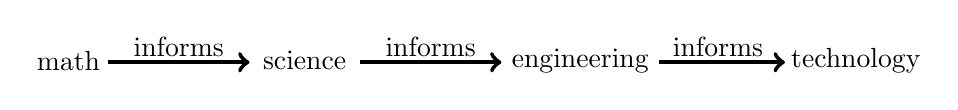
\begin{tikzpicture}
                    \node [align=center] at (0.0, 0.02){math};
                    \draw [ultra thick, ->] (0.5, 0) -- (2.3, 0);
                    \node [align=center] at (1.4, 0.2){informs};
                    \node [align=center] at (3.0, 0.02){science};
                    \draw [ultra thick, ->] (3.7, 0) -- (5.5, 0);
                    \node [align=center] at (4.6, 0.2){informs};
                    \node [align=center] at (6.5, 0.02){engineering};
                    \draw [ultra thick, ->] (7.5, 0) -- (9.1, 0);
                    \node [align=center] at (8.25, 0.2){informs};
                    \node [align=center] at (10, 0.02){technology};
                \end{tikzpicture}
            \end{figure}
                
            However, you'll also find that philosophy informs all of these, and is informed by all of these. The creative arts, like philosophy, is informed by all 4 of these, but tends towards informing only engineering and technology.
                
            This does not mean that mathematics and science is not creative, but it's often misunderstood that because mathematics is so rational, that it's not creative. It takes a lot of creative thinking and intuition, along with rational thought, in order to come up with mathematical proofs, and it is for this reason, and the connections to other fields, that creative arts is a necessary endeavour for anyone learning STEM.
                
            In fact, this is precisely the argument for STEAM.
                
            It must be stated more clearly, because the previous statement may not be clear enough: creative thinking, intuition, and rational thinking are \textbf{all} required for work in each of these fields of study, in concert with each other. Rational thinking does not promote mathematics and science alone. Intuitional thinking will almost certainly lead to falsehoods in these fields, if not matched with rational thinking.
                
            In this sense, creative thinking can be seen to be exploration, finding solution-after-solution, intuitive thinking can be seen to point the creative thinking along, but the rational thinking is the filter that finds the solutions that actually work.
                
            So, you will benefit all of these parts of your mind, including the part of you that is disciplined and builds grit. This will happen by mere practice and use, much like a muscle being used over-and-over getting bigger, and capable of handling more.
                
            Mathematics and the sciences change how you look at the world around you, but it doesn't make you a better person.
        \end{subsection}
        
        \begin{subsection}{The Danger in Strength}
            Philosophy has a long history of beneficial usage and of dangerous misuse. Philosophy may be the most important, but the most dangerous subject matter that a mind can consume. Philosophy has been used to free people as well as enslave people. The philosophical concept of moral or ethical \emph{justification} has been used both to protect and to kill.
            
            In effect, every argument about whether or not human beings are ready for a specific technology is actually a question of whether or not human beings are philosophically mature enough, and is captured in the following quotes:
            
            \begin{quote}{Jason Silva}
                Technology is, of course, a double-edged sword. Fire can cook our food but also burn us.
            \end{quote}
            
            \begin{quote}{Christian Lous Lange}
                Technology is a useful servant, but a dangerous master.
            \end{quote}
            
            \begin{quote}{B. F. Skinner}
                The real problem is not whether machines think, but whether people do.
            \end{quote}
            
            Replace ``technology'' with ``philosophy'' in the first two quotes, and you may begin to understand what it is that I'm claiming. Other quotes are a bit more direct:
            
            \begin{quote}{Martin Luther King, Jr}
                Nothing in all the world is more dangerous than sincere ignorance and conscientious stupidity.
            \end{quote}
            
            \begin{quote}{George Bernard Shaw}
                Beware false knowledge; it is more dangerous than ignorance
            \end{quote}
            
            \begin{quote}{Confucius}
                Real knowledge is to know the extent of one’s ignorance
            \end{quote}
            
            Oftentimes, it is exactly those strengths that serve as one's weaknesses, but that is not to say that having a strength necessarily creates weakness in that area. It benefits us to understand how strengths become weaknesses. 
    
            Philosophy, like technology, is good or bad, depending on how it's used, and depending on how well it's understood, and based on what principles one chooses to work from.
                
            In fact, the call-to-action I give each of you, before you start this endeavour is:
            \begin{itemize}
                \item Use your observations and experiences to help you understand your world
                    
                \item Uproot misperceptions and misunderstandings that come from a partial understanding of the first
                    
                \item Apply your understanding of the world to better your world and the world of others, as you see fit
            \end{itemize}
        \end{subsection}
        
        \begin{samepage}
            \begin{subsection}{Perceptions and Misperceptions of Philosophy, Mathematics, and Science}
                There are multiple misperceptions of about various fields of study, such as:
                \begin{itemize}
                    \item Mathematics
                    \begin{itemize}
                        \item It's not a creative field
                        \item It's the study of numbers
                        \item It's already finished (there's no new math to be had)
                        \item There are no jobs for mathematicians
                    \end{itemize}
                    
                    \item Science
                    \begin{itemize}
                        \item It's done by elite people who have no connection to reality
                        \item It's a collection of statements that are considered ``the truth''
                        \item It doesn't help ``real people''
                    \end{itemize}
                    
                    \item Software Development
                    \begin{itemize}
                        \item It's all copy-and-paste
                        \item Computers will be programming themselves soon
                        \item It's an easy desk-job with little pressure
                    \end{itemize}
                        
                    \item Economics
                    \begin{itemize}
                        \item It's the study of money
                        \item It's all psychology (which contradicts the first claim)
                    \end{itemize}
                \end{itemize}
            \end{subsection}
        \end{samepage}
            
        All of these claims are caricatures of the fields of study, or of the people who do work in those fields, and are not just oversimplifications, but are outright wrong if one were to actually follow these people around.
            
        Much the same misrepresentation occurs in all fields of study and all fields of work. These misrepresentations continue throughout the centuries as populism attempts to change the view of these subjects.
            
        The history of this populism is understood, because in history, fields such as these could only be achieved by the educated and the rich, and those people would not understand those who worked with their hands. Therefore, a schism occurred between those who used their minds, and those who used their hands, based on a classism that is not yet resolved.
            
        A shift has been occurring over the last few centuries though, especially as education has become more universal, allowing people to spend part of their lives in service, part of their lives in manual labor, part of their lives studying, and part of their lives working with their minds, and it's not certain that a person in any particular job has any particular experience.
            
        In this regard, philosophy has always been misrepresented, and you may hear things like:
        \begin{enumerate}
            \item Philosophy, like mathematics, has been completed, or it has produced all of the results and discoveries that it can
                
            \item Philosophy is useless, ungrounded, and a waste of a person's education
                
            \item Philosophy is nebulous, vague, and done by people who are out-of-touch with the real-world
                
            \item Philosophy opposes, is not supported of, or is somehow separate from science
        \end{enumerate}
            
        Nothing could be further from the truth on all of these grounds. Mathematics, and philosophy, are coming up with new discoveries all the time, and including applications to previous discoveries. Philosophy, especially the interest of how we come to know things, forms the basis for both mathematics and the sciences.
    \end{section}
    
    \begin{section}{What is Philosophy, and Why Should We Care?}
        Philosophy is typically introduced by discussing what it means, and where it comes from. We focus so much on the Greek philosophy, but philosophy, mathematics, and science has been growing in all cultures for millennia, and can be found as early trial versions of these subjects in ancient books all over the world.
            
        The word ``philosophy'' is a word from ancient Greek φιλοσοφία (\emph{philosophía}), which has 2 roots:
        \begin{itemize}
            \item φίλος (phílos meaning “loving”)
            \item σοφία (sophía meaning “wisdom”)
        \end{itemize}
            
        However, that only scratches the surface, and tends to lead to the conclusion that “philosophy is in every query”. Although this is technically true, it does little to give anyone any clue to what philosophers actually do, and why it’s important.
            
        In some ways, philosophy is the process of exploring one’s thoughts, asking ourselves, “why do I think this way?”
            
        Specifically, philosophers have certain question that all philosophy branches out from:
            
        \begin{figure}[ht]
            \centering
            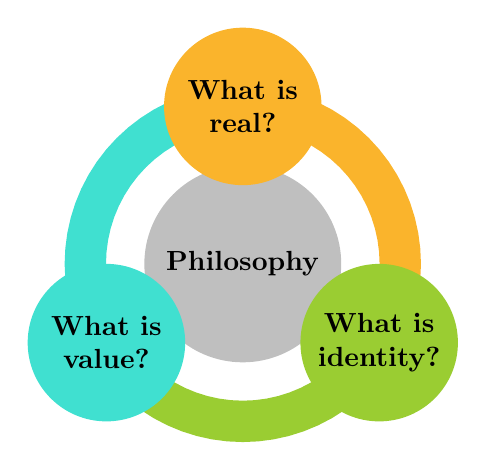
\begin{tikzpicture}
                \fill [lightgray]   (0,0) circle (12.5mm);
                \node [align=center] at (0, 0) {\textbf{Philosophy}};
                \draw [Dandelion,line width=5.25mm,domain=-30:90] plot ({2*cos(\x)},     {2*sin(\x)});
                \draw [YellowGreen,line width=5.25mm,domain=210:330] plot ({2*cos(\x)},     {2*sin(\x)});
                \draw [Turquoise,line width=5.25mm,domain=90:210] plot ({2*cos(\x)},     {2*sin(\x)});
                \fill [Dandelion] (0,2) circle (10mm);
                \fill [YellowGreen] ( 1.732,-1) circle (10mm);
                \fill [Turquoise]   (-1.732,-1) circle (10mm);
                \node [align=center] at ( 0.000, 2) {\textbf{What is}\\\textbf{real?}};
                \node [align=center] at ( 1.732,-1) {\textbf{What is}\\\textbf{identity?}};
                \node [align=center] at (-1.732,-1) {\textbf{What is}\\\textbf{value?}};
            \end{tikzpicture}
            \caption{The 3 Proposed Root Questions of Philosophy.}
            \label{fig:ThreePhilosophicalQuestions}
        \end{figure}
            
        Here though, these 3 questions feed off of each other. For instance, 
        \begin{itemize}
            \item Is it possible to seek truth without asking what methods of truth-seeking that we value?
                
            \item If something exists (if it’s “real” or “true”), can we identify it?
                
            \item If we change something (identity) does it change value?
        \end{itemize}
            
        In fact, these three questions spawn multiple branches of study, some of which are considered philosophical in modern times still, others may appear, on the surface, as if they are something separate from philosophy.
            
        \begin{subsection}{What is Real?}
            Epistemology relates to the question, “How do we know what we know?”. The study     of epistemology has given us logic (forming the foundations of mathematics),     the Scientific Method (forming the foundations of science), and gives us     mechanisms for us to understand beliefs by asking:
                
            \begin{itemize}
                \item What does it mean to know something?
                \item Can anything be known for certain? 
                \item How much confidence can we have in something?
                \item What is the process that we come to know things?
                \item What does it mean to know things?
                \item What is a belief?
                \item Can we justify our beliefs? (\textbf{critical reasoning})
                \item What is the relationship between beliefs and knowledge?     (\textbf{doxastic logic})
            \end{itemize}
        \end{subsection}
            
        \begin{subsection}{What is Identity?}
            In philosophy, we talk about \textbf{discernibility}, which lets us ask, “if two things share all the same properties, are they the same thing?”. We use this in mathematics to present two things being equal. In science, we identify phenomena that interest us. In our lives, we discuss personal identity, social identity, and even discuss the human identity. In many ways, the philosophical focus on definitions and on meanings are directly related to identifying concepts, and coming to agreement on concepts, in order to help discuss.
                
            It leads us to questions like:
                
            \begin{itemize}
                \item What does it mean for two things to be the same, and does that change over time or based on the context?
                \item If I replace every component with an identity component, is it the same thing (Interchangeability and compatibility)?
                \item Are we the same person from one moment to the next?
                \item Is any object the same from one moment to the next?
                \item How do we relate to and do we identify with our city, our culture, and/or our nation?
                \item What does it mean when things are “almost alike” or similar? And do similar things share similar properties?
            \end{itemize}
        \end{subsection}
        \begin{subsection}{What is Value?}
            The notion of \textbf{value} or \textbf{worth} is also of central concern, as it allows us to compare two things. This is also of central concern in mathematics as it allows us to make statements about relationships between things. It is of concern in modern politics, when discussing the value of citizens and whether or not they feel valued. We discuss \textbf{aesthetics} as the study of those things that attract our senses. We discuss \textbf{ethics} through the value of actions. It leads us to questions like:
                
            \begin{itemize}
                \item What does it mean to compare two things?
                \item Why do things cost what they do?
                \item What do individuals value, and why?
                \item What do societies value, and why?
                \item Is something practical worth more than something else? What makes it practical?
                \item What is fairness and justice?
            \end{itemize}
        \end{subsection}
        \begin{subsection}{What is the Relationship Between Value and Identity?}
            When questions about both value and identity come together, we usually start to ask about purpose, and
            \begin{itemize}
                \item Is there a purpose to the existence of the universe? What is the purpose?
                \item Is there a purpose to my existence? What is the purpose? Do I create my own purpose?
                \item Am I a valued part of my community? Why or why not?
                \item What is fair when it comes to treatment of different people?
                \item How does interchangeability relate to comparison? If I interchange components for something newer, is it better?
            \end{itemize}
        \end{subsection}
        \begin{subsection}{What is the Relationship Between Value and Truth?}
            This is the intersection of the two questions that lead us to asking questions like:
            \begin{itemize}
                \item How do we value the various means of obtaining knowledge?
                \item How do people value methods of communicating knowledge and beliefs?
                \item Whose testimonies do we believe and why?
                \item Can there be an absolute, top-level truth, by which all other truths are measured?
                \item Can there be a best moral code, by which all other moral codes are measured?
            \end{itemize}
        \end{subsection}
        \begin{subsection}{What is the Relationship Between Identity and Truth?}
            Regarding identity and truth, we may get some interesting questions about ourselves and:
            \begin{itemize}
                \item What are we? (i.e. what makes us human, or what makes us different?)
                \item Where do we come from?
                \item Why does anything exist at all?
                \item How do we relate to our perceptions, and vice versa?
                \item What does it mean to “exist”?
                \item What does it mean to be “real”?
                \item What is reality?
                \item What is the mind?
            \end{itemize}
        \end{subsection}
        \begin{subsection}{What is the Relationship Between All 3?}
            Finally, we can consider all 3 together:
            \begin{itemize}
                \item Is there something bigger than us?
                \item What is out there, beyond what we can perceive?
                \item How did this universe come to exist? (\textbf{cosmology})
                \item What is the greatest possible mind? Must a creator exist? (\textbf{theology})
            \end{itemize}
        \end{subsection}
            
        \begin{subsection}{Categorizing the Questions into Branches}
            Many of these questions have been placed into various categories:
            \begin{itemize}
                \item That reason can be a source of knowledge (\textbf{rationalism}) allowed us to create logic, and logic continues to refine the foundations of mathematics (classically called, “the formal sciences”)
                    
                \item Critical thinking, using our senses as a source of knowledge (\textbf{empiricism}), building confidence through experimentation (\textbf{verificationism}), and filtering in only those things that we can derive from these sources (\textbf{positivism}) refines the scientific method, which gives us science (classically called, “the physical sciences”)
                
                \item Questions about value form the basis for \textbf{Value Theory}, and include subbranches like: ethics, aesthetics, and axiology (moving into application through economics and politics)
                    
                \item Questions about existence and reality form the basis of \textbf{Metaphysics}, and include subbranches like: theology, religion, and ontology 
                    
                \item Questions about how we do philosophy form the basis of \textbf{Metaphilosophy}
            \end{itemize}
        \end{subsection}
    \end{section}
    
    \begin{section}{Philosophical Discussions}
        So, you thought that this book was going to be about mathematics. Why, then, are we learning philosophy? Well, it turns out that philosophy is the parent of almost every subject studied in any formal education. 
            
        Given that we have asked about reality, science is a formal discipline of the philosophical position called empiricism, allowing us to enter into discussion about those areas of discussion that can be observed and measured with repeatable results. However, as positions go, science is limited to such discussions.
            
        Foremost, we are interested in mathematics in this book, but we will only really get there by discussing the roots of mathematics. Also, in order to understand it, we will do best when we can also link our study to various other areas as well. The most interesting part is how these things link.
            
        \begin{figure}[ht]
            \centering
            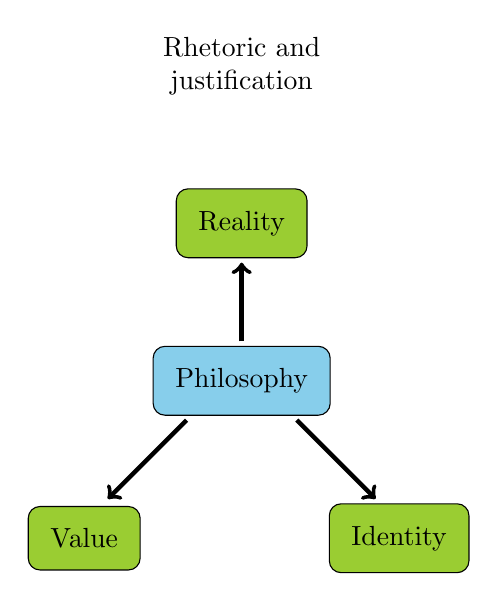
\begin{tikzpicture}
                \node [align=center,draw=black,fill=SkyBlue,thin,inner sep=8pt,rounded corners=.15cm] at (0.0, 0.0) {Philosophy};
                
                \node [align=center,draw=black,fill=YellowGreen,thin,inner sep=8pt,rounded corners=.15cm] at (0.0, 2.0) {Reality};
                
                \node [align=center] at (0.0, 4.0) {Rhetoric and\\justification};
                
                \node [align=center,draw=black,fill=YellowGreen,thin,inner sep=8pt,rounded corners=.15cm] at (-2, -2.0) {Value};
                
                \node [align=center,draw=black,fill=YellowGreen,thin,inner sep=8pt,rounded corners=.15cm] at ( 2, -2.0) {Identity};
                
                \draw [ultra thick, ->] ( 0.0, 0.5) -- (0.0, 1.5);
                \draw [ultra thick, ->] (-0.7,-0.5) -- (-1.7, -1.5);
                \draw [ultra thick, ->] ( 0.7,-0.5) -- ( 1.7, -1.5);
                %\node [align=center] at (0.0, 0.02){math};
                %\draw [ultra thick, ->] (0.5, 0) -- (2.3, 0);
                %\node [align=center] at (1.4, 0.2){informs};
                %\node [align=center] at (3.0, 0.02){science};
                %\draw [ultra thick, ->] (3.7, 0) -- (5.5, 0);
                %\node [align=center] at (4.6, 0.2){informs};
                %\node [align=center] at (6.5, 0.02){engineering};
                %\draw [ultra thick, ->] (7.5, 0) -- (9.1, 0);
                %%\node [align=center] at (8.25, 0.2){informs};
                %\node [align=center] at (10, 0.02){technology};
            \end{tikzpicture}
        \end{figure}
            
        \begin{figure}[H]
            \centering
            \includegraphics[scale=0.65]{PhilosophicalIntroduction/ConnectionsToPhilosophy.png}
            \caption{Connections of Various Fields to Philosophy.}
            \label{fig:ConnectionsToPhilosophy}
        \end{figure}
            
        \begin{subsection}{Rhetoric and Justifying Beliefs}
            It's important to understand that much of our mental sophistication revolves around explaining ourselves to others, whether that be in regards to giving them a mental image of what we have seen, explaining how something works, to justifying our reasons for doing something.
                
            Jonathan Haidt gave us the analogy of our minds being of a human rider on top of an elephant, whereas the rider is the rational mind, and the intuition is the elephant. We are so good at justifying our actions to others, that we often justify things we have done to ourselves, even when we know better (e.g. ``I can eat that whole chocolate cake, because I've done so well on my diet this week.'').
                
            Our written Greek philosophy seems to start with regards to \textbf{rhetoric}, as the ``art of discussion'', developing the communication skills to discuss philosophical positions.
                
            Rhetoric was often divided into:
            \begin{itemize}
                \item \textbf{Emotional} appeals, intended to speak directly to the mind's elephant. These appeals are often highly effective, if sometimes manipulative in their usage.
                    
                \item \textbf{Authoritative} appeals, intended to invoke the authority of the speaker, through their experience or due to their character-history of truthfulness.
                    
                \item \textbf{Rational} appeals, intended to speak directly to the rider of the elephant, who is capable of mapping out a direction for the elephant to travel, if the rider can ever get the elephant to listen.
            \end{itemize}
                
            We may be used to hearing the word rhetoric in political discussions (such as ``inflammatory rhetoric''), but oftentimes the person using the word doesn't mean it with the nuance of the philosophical meaning. Instead, philosophers would deem what politicians are doing \textbf{polemic}, which is emotional arguments intended to reduce confidence in and incite fear of an opponent.
                
            It should be obvious that mathematics and the sciences are filled with logical appeals, and as such, this book will be filled with them as well. However, it's also recognized that the intuition must be brought on board as well. 
                
            Finally, the authoritative appeals should be mostly unused in any discussion of mathematics. There is no for a teacher to use appeals to authority, saying things like ``it just works this way''. The only authoritative appeals will be the usage of already defined and commonly used standards for writing that may be brought up. However, even those should be backed with arguments for rational reasons why.
                
            \begin{subsubsection}{Some Definitions}
                
                \begin{definition}
                    An \textbf{interlocutor} is a person that is taking part in a dialog.
                \end{definition}
                    
                \begin{definition}
                    A \textbf{proposition} is a statement is possibly true or false.
                \end{definition}
                    
                \begin{definition}
                    A \textbf{premise} is a proposition for consideration, sometimes asserted as true by the interlocutor, and sometimes as a condition for the context of the argument.
                \end{definition}
                    
                \begin{definition}
                    A \textbf{conclusion} is a proposition that is the end result that the interlocutor reaches starting from the premises.
                \end{definition}
                    
                \begin{definition}
                    An \textbf{argument} is a series of propositions, structured such that the premises lead to a conclusion. Furthermore, a more general meaning of this word may be a process of reasoning.
                \end{definition}
                    
                \begin{definition}
                    A premise taken as a condition, usually in regards to an investigation is called a \textbf{hypothesis}.
                \end{definition}
                    
                \begin{definition}
                    A \textbf{philosophical position} is a collection of premises that an interlocutor is arguing from.
                        
                    It is often called a \textbf{philosophical theory}, which can cause confusion with the significantly different meanings taken by scientific theory and mathematical theory. 
                        
                    The everyday usage of the word ``theory'' is probably best identified as ``hypothesis''.
                        
                    Due to this confusion, the word position will be preferred in this book.
                \end{definition}
                    
                \begin{figure}[ht]
                    \centering
                    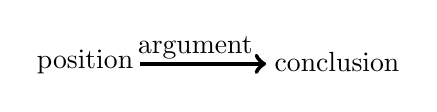
\begin{tikzpicture}
                        \node [align=right] at (0.0, 0.02){position};
                        \draw [ultra thick, ->] (0.7, 0) -- (2.3, 0);
                        \node [align=center] at (1.4, 0.2){argument};
                        \node [align=left] at (3.2, 0.02){conclusion};
                    \end{tikzpicture}
                    \caption{Relation between position (premises), argument, and conclusion}
                \end{figure}
                    
                \begin{definition}
                    For the sake of comparison, a \textbf{life stance} is a philosophical position that one takes, according to their worldview, which informs their beliefs, their thoughts, and their behavior.
                        
                    This is stated separately, since a life stance differs from a philosophical position.
                \end{definition}
                    
                \begin{definition}
                    A \textbf{Devil's Advocate} is a person that argues from a position that differs from their life stance, in order to better understand their own position, and the position of others.
                \end{definition}
                    
                \begin{definition}
                    \textbf{Skepticism} is the act of reserving belief for future evidence.
                \end{definition}
                
                \begin{definition}
                    \textbf{Belief revision} is the act of modifying one or more premises that make up a position, due to new evidence.
                \end{definition}
            \end{subsubsection}
            
            \begin{subsubsection}{What Forms a Worldview}
                At this point, I'm going to present what follows as a position, setting the rest of the book up for discussions on logical reasoning.
                    
                \begin{remark}
                    This position I am starting from, regarding worldviews, is not scientific, is not based on psychological evidence, and is likely just an approximation of how worldviews actually work.
                \end{remark}
                    
                \begin{figure}[ht]
                    \centering
                    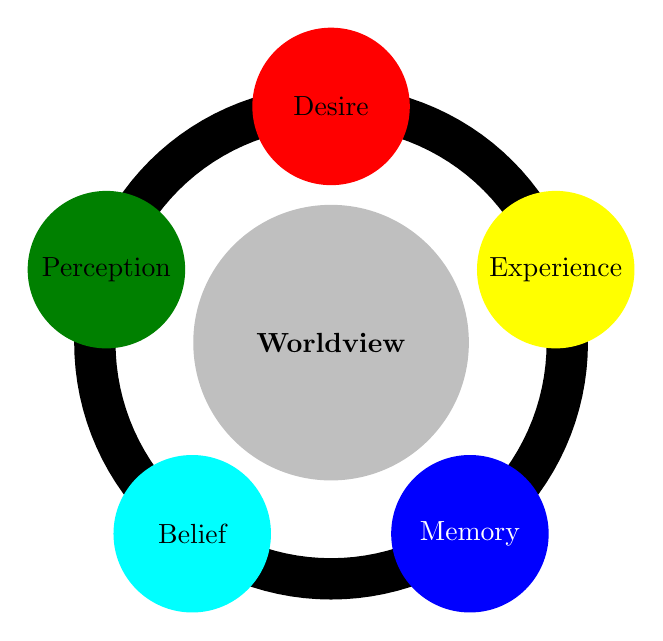
\begin{tikzpicture}
                        \fill [lightgray] (0,0) circle (1.75cm);
                        \node [align=center] at (0, 0) {\textbf{Worldview}};
                            
                        \draw [Black,line width=5.25mm,domain=90:162] plot ({3*cos(\x)}, {3*sin(\x)});
                        \draw [Black,line width=5.25mm,domain=162:234] plot ({3*cos(\x)}, {3*sin(\x)});
                        \draw [Black,line width=5.25mm,domain=234:306] plot ({3*cos(\x)}, {3*sin(\x)});
                        \draw [Black,line width=5.25mm,domain=306:378] plot ({3*cos(\x)}, {3*sin(\x)});
                        \draw [Black,line width=5.25mm,domain=378:450] plot ({3*cos(\x)}, {3*sin(\x)});
                            
                        \fill [Red]   ( 0.000000, 3.000000) circle (10mm);
                        \fill [Green] (-2.853170, 0.927051) circle (10mm);
                        \fill [Cyan]  (-1.763356,-2.427051) circle (10mm);
                        \fill [Blue]  ( 1.763356,-2.427051) circle (10mm);
                        \fill [Yellow]( 2.853170, 0.927051) circle (10mm);
                            
                        \node [align=center,text=black] at 
                        ( 0.000000, 3.000000) {Desire};
                        \node [align=center,text=black] at 
                        (-2.853170, 0.927051) {Perception};
                        \node [align=center,text=black] at 
                        (-1.763356,-2.427051) {Belief};
                        \node [align=center,text=white] at 
                        ( 1.763356,-2.427051) {Memory};
                        \node [align=center,text=black] at 
                        ( 2.853170, 0.927051) {Experience};
                    \end{tikzpicture}
                    \caption{Relation between position (premises), argument, and conclusion}
                \end{figure}
                    
                The first question someone may have looking at the components of a person's worldview that I listed is that experience, memory, and belief are all the same thing. However, my argument is that we experience all the time, but our beliefs color how we interpret the memories associated with those experiences.
                    
                In this sense, we reexperience things through our memory, but it doesn't mean that it feels the same each time.
                    
                It may seem strange that I put desire in with the rest of these, because it appears that the rest of these relate to knowledge, but that desire is completely unrelated. However, we already know that desires change how we perceive things, making us more or less perceptive of our failures or successes, or how other people act.
                    
                The point of all of this is to say that our memories are fallible, because they change. Our perceptions are fallible as well, and so, we cannot always trust our worldview.
            \end{subsubsection}
                
            \begin{subsubsection}{What Sources of Information do you Value?}
                In the discussion of rhetoric, we talked about 3 different types of arguments: emotional, authoritative, and rational.
                    
                However, these are only the methods of transference of information from one person to another, and misses an important source of information: experience.
                    
                We tend to regard experience as the most valued source of information, but as we discussed in regards to the worldview, our perceptions of experiences are often incomplete, and sometimes even wrong.
                    
                Most people, naturally value emotional, authoritative, experiential, intuitive, and rational information sources to some level or another, because we naturally recognize that there are failings with putting all of our trust in any one of them: emotions can sometimes be erratic, people sometimes lie, our perceptions often deceive us, our intuitions are often wrong, and we often don't have enough information to come to a rational conclusion.
                    
                However, there are things that we can do to refine when we use each, and what we can be said about each source of information.
                    
                Firstly, it's important to note that rational arguments begin as intuitive arguments. Humans have an intuitive ability to recognize cause-and-effect, allowing us to determine how things work, and often change how things work to our favor. This recognition of the pattern of cause-and-effect is what leads us to logic, and rational thinking is the disciplined use of this logic. 
                    
                In fact, the discipline is what separates intuition from rational thinking. We follow through with our intuitions to see if they fail.
                    
                Second, the relationship between emotions and intuition are also important. Purely rational thinking is devoid of creativity, can get stuck in analysis, and therefore absent problem solving ability. However, purely intuitive thinking cannot weed out those ideas that won't work, and will naturally try things that are not logically sound, usually wasting their own and other people's time.
                    
                First, let's get more detailed how these each operate as a source of information:
                \begin{itemize}
                        
                    \item Authoritative sources
                    \begin{itemize}
                        \item \textbf{Witnesses} can provide accounts of events
                        \item Parents and teachers often provide us tons of information
                    \end{itemize}
                    \item Experiential sources
                    \begin{itemize}
                        \item Your \textbf{senses} give you access to the world around you and are your connection to it
                        \item When your senses act together they create an \textbf{empirical} view of the world
                        \item This effectively places you as an authority over your own worldview
                        \item Demonstrations from other individuals can help communicate subject matter
                    \end{itemize}
                    \item Emotional and Intuitive sources
                    \begin{itemize}
                        \item Emotions can point us to how our intuitions react to specific experiences
                        \item Gut feelings can tell us things about our world, and are frequently part of our mental pattern-matching capabilities.
                        \item It is via these gut feelings that we are capable of walking, knowing where to place each foot as we move
                        \item The intuitive is unconscious, but quick to form conclusions
                    \end{itemize}
                    \item Rational sources
                    \begin{itemize}
                        \item We use logic and probability to determine whether or not something is possible
                        \item We use analogy to compare and contrast things that we know against things that we do not know
                    \end{itemize}
                \end{itemize}
                    
                We know that authorities can lie, and that witnesses can't always trust their memories. Likewise, we cannot always trust our senses, nor our memories. Our emotions and intuitions are often wrong. Also, we can misuse logic, probability, and analogy.
                    
                In seeking information that we can trust, it seems like we are out of luck, but through careful inspection, we can begin to clear out the mess.
                        
                Regarding rational and intuitive thought, if we learn how to properly use logic and to understand our own biases, we can balance intuition with rational thinking, by allowing intuition to come up with hypotheses, and cutting through the wrong ones via rational thought. We can learn how where rational thinking works, and how sometimes fails us.
                    
                Regarding experience, we can learn about our own psychology, and also through our biases, determine when we can trust our senses and our experiences. We can determine whether multiple memories working together with evidence can corroborate our hypotheses.
                    
                Regarding authorities, \textbf{Subject Matter Experts} are people who are experienced in a subject matter and have a record of insightful discussions, and as long as they have no motive to lie to us, information inside their area of expertise can be trusted.
                    
                From there, we can actually learn what authorities know, how they came to their conclusions, and come to conclusions ourselves via experience and rational thinking.
                    
                So, it's important to think about how and why you value the sources of information that you do, how and why they can fail you, and how to effectively work through them.
            \end{subsubsection}
                
            \begin{subsubsection}{Epistemology}
                The study of what we know and how we come to know it is called \textbf{epistemology}. It is extremely important in the realm of mathematics and the sciences to understand epistemology, 
            \end{subsubsection}
            \begin{subsubsection}{Rigorous Communication}
                Furthermore, most of this communication between experts requires that the words they use are well-understood. We have definitions for words that we use all the time, but often words in a particular \emph{subject matter} have explicit definitions which differ from how they are used in everyday speech.
                    
                Let's consider one of the most problematic words in use today. The word \textbf{theory} from the ancient Greek θεωρία (``theoria'') was contrasted to πρᾶξις (``praxis'' where we get the word ``practice''). The theory behind something was the contemplation regarding how an activity works, and the praxis was the act of doing it. Therefore, theory was used to improve the praxis, but praxis was used to improve the theory.
                    
                This contrasting terminology between the two is why we still have phrases like ``that's works in theory, but not in practice''. However, the meaning of theory in our everyday life is not necessarily how it is used elsewhere:
                    
                \begin{itemize}
                    \item \textbf{Theory (science)} -- a hypothesis which is confirmed by repeated and thorough experimental observation to provide reliable predictions
                    
                    \item \textbf{Theory (mathematics)} -- the collection of premises and conclusions related specific mathematical structures
                        
                    \item \textbf{Theory (philosophy)} -- the collections of premises and conclusions specific to an area of philosophical pursuit (also called a philosophical position).
                        
                    \item \textbf{Theory (everyday speech)} -- a proposed explanation serving as a hypothesis
                \end{itemize}
            \end{subsubsection}
                
                
        \end{subsection}
        \begin{subsection}{Ontology and the Mathematics of Identity, Equality, and Equivalence}
            Discernibility
            Distinguisibility
            Interchangeability
            Identical
                
            \begin{subsubsection}{Definitions}
                In every field of study, we have to be extremely careful what it is we mean when we say something, and aim to avoid
                    
                In mathematics, we often define something, to use in a context (a scope of discussion) and when we are done, we stop meaning it the same. In speech, we do this often with pronouns. For instance, ``Caleb left work. He wasn't feeling that well.''. We immediately know that `He' in the sentence refers to Caleb. In this case, with English, we didn't even specifically define that we'd use `He' this way.
            \end{subsubsection}
                
                
            \begin{subsubsection}{Isomorphisms}
                \begin{definition}
                    The word \textbf{isomorphism} has a formal definition that we will cover later in Category Theory. Philosophically, it can be thought best to first recognize that mathematical objects are conceptual, not physical, and we can argue only that two objects constructed exactly the same way (structural identity) are identical. However, as we have said, two objects can be constructed in 2 different ways and behave as if they are the same object. These objects then have interchangeability between them.
                    
                    An isomorphism focuses, not on identical constructions (what the objects ``are''), but on identical behaviors (what the objects ``do''), and more specifically, that they adhere to the same ``legal contracts'' we call axioms.
                    
                    The word isomorphism (iso- ``same'', -morphism ``form'') is an effective ``equality between types of things''. 
                \end{definition}
                
                An example would be the 2 identical definitions for the number 1:
                \begin{enumerate}
                    \item The natural number comes after 0
                    \item The unique natural number that allows us to multiply any number by itself and result in the same number
                \end{enumerate}
                
                Both of those definitions for 1 focus on what it does, but the first definition is closer to the actual construction of 1 than the second. The two definitions are isomorphic to each other.
                    
                Furthermore, we have the Univalence Axiom, which binds multiple mathematical fields together, in the same way that René Descartés bound algebra together with geometry when he noticed that we can put things on a grid. The proposal of the Univalence Axiom first observed that equivalence (structural identity) implies isomorphism(interchangeability), but the true observation was that an isomorphism was interchangeable with an equivalence.
                
                Now, that's not being fully honest, and yet it is at the same time. A good philosopher will think to themselves, ``you didn't use the word `equivalence' the same way in both of those sentences'', and that philosopher would be right.
                
                I started the discussion talking about identical constructions (what objects ``are''),and obviously, two things cannot be equivalent if they do not have identical constructions. However, equivalence doesn't have to mean identical constructions.Mathematicians often define equivalence based on interchangeability in the same sense as the following analogy:
                
                \begin{quote}
                    A ``Gizmo'' machine has a component called a ``doohickey''. If I can take the doohickey out and replace it with another doohickey, they are interchangeable. If I can replace the Gizmo with another Gizmo, and use the same doohickey in both, then the Gizmo itself is fungible (interchangeable with other things that use components). If any doohickey can go in any Gizmo, then the differences between each doohickey is indiscernible.
                \end{quote}
                
                So, we get an isomorphism between algebraic equations and geometry from Descartés. From Euler we'll see how trigonometry, calculus, and complex numbers relate. However, here we use this opportunity to note that there is an isomorphism between paths, logic,partial orders, computation (and computer science), and tons of things we may get to later, just from Vladimir Voevodsky's Univalence Axiom.
                
                Finally, I have mentioned Axioms as ``legal contracts for mathematical structures''.You may be asking, what structure do we assume Univalence for? We will eventually get into Category Theory, and that will help combine all the world of mathematics together for us.
                
                So, it helps to understand that equality has context, just as isomorphism has context, and we may discuss various types of equalities.
            \end{subsubsection}
                
            \begin{subsubsection}{Natural Numbers are not Non-negative Integers}
                Never does the distinction and non-distinction matter as much as how we teach the number classifications. We have probably been taught that we can identify integers as allowing for negative numbers, and that every natural numbers \textbf{is} an integer.
                    
                This notion of \textbf{is} refers to our isomorphism from earlier. We can construct integers, and we can construct natural numbers, and we will construct them later, but the statement ``\textbf{is}'' used above must be understood to mean that we can get an integer from a natural number, and take that same integer and find a natural number that matches it. That is what it means to ``be the same''.
            \end{subsubsection}
        \end{subsection}
    \end{section}
\end{chapter}
\chapter{Logical Deduction}
\section{Classical Logic}
Socrates tells us that Plato gave us 3 \gls{LawsOfThought} (paraphrased here, and using the notion of ``true'' as a value):
\begin{itemize}
\item \textbf{Law of Identity} –- For any statement P, P = P. This is to say that true is true, false is false, and this law basically defines a notion of equality for logic.
\item \textbf{Law of Non-Contradiction} –- No two contradictory statements can both be true. For instance, it cannot be that ``Humans are animals'' and ``Humans are not animals''.
\item \textbf{Law of the Excluded Middle} –- Everything must be either true or false.
\end{itemize}

There are also records of the Law of Non-Contradiction in the Indian Sutras, but the most well-known collection of these 3 laws is by Socrates.
Aristotle also gave us one more law, codified as the \textbf{syllogism}:
If we have the following two statements:
\begin{itemize}
\item If X then Y
\item X
\end{itemize}
Then we can conclude Y; and hence, justification in intuitionistic logic is interpreted as “reachability”, the ability to reach Y from X.

An example of a syllogism would be, “If it is raining in the open field, then the ground is getting wetter”, and “it is raining” giving us the result that “the ground is getting wetter”

Now, it may seem counterintuitive, but we cannot conclude the logical converse (swapping). In other words, we cannot use wet ground to conclude that it is raining, because sprinklers may be on, or the water hose running over the ground.

\todo{treat it like a path}
\chapter{Boolean Logic}
\section{The Boolean Domain}
We often talk about different structures in mathematics, starting with what possible values it can have. The \gls{BooleanDomain} is used to describe something that has 2 possible values, but also interpret
one value as \emph{true} and the other as \emph{false}.

Following the discussion of Classical Logic, the Boolean Domain represents the possible values that Classical Logic can have, since Classical Logic uses the Law of the Excluded Middle to claim that there
are only 2 possible values.

When we are working with the Boolean Domain, we call a possible element a \gls{bit}.
\subsection{Symbols for Elements}
There are numerous ways to represent the Boolean Domain, and some can be interpreted below:
\begin{table}[ht]
\centering
\begin{tabular}{|c|c|c|c|c|}
    \hline
    False & 0 & $\bot$ & F & \texttt{-}1 \\ \hline
    True  & 1 & $\top$ & T & \texttt{+}1 \\ \hline
\end{tabular}
\end{table}

Each has a use that makes more sense in some situations over others. In this book, we will typically use T and F as the 2 values used to describe \emph{true} and \emph{false} respectively, but here is how the others may be used:

\begin{itemize}
    \item 0 and 1 are used in computers, and represent values that mean that a circuit is enabled (1) or disabled (1). Of course, we can reverse the meaning of these two, but typically enabled and disabled are 1 and 0 respectively.
    
    \item $\bot$ and $\top$ are used to demonstrate that Boolean Logic is symmetrical, in a way that will be described later.
    
    \item \texttt{-}1 and \texttt{+}1 are used rarely to demonstrate how Boolean Logic can be viewed in a way similar to arithmetic.
\end{itemize}

\subsection{Symbols for the Domain Itself}

The symbol for the Boolean Domain itself is $\mathbb{B}$. The elements will be referred to as T and F. Therefore, we will later make frequent use of symbolic relations like the following:

$$
    \mathbb{B} = \{T, F\}
$$

Which means to say that the Boolean Domain ($\mathbb{B}$) is ($=$) the set of items with a true and false ($\{T, F\}$).

\section{Interpretation as Logical True and False}
To interpret the values T as having logical truth is to also say that T is more true than F is. It may at first seem like mathematics says a lot off obvious things, but sometimes it needs to be stated for other conclusions to be made.

With that interpretation in mind, we can then make philosophical claims. We used the claim that ``When it is raining, the uncovered ground is getting wetter'' before, and we can use ``p'' to mean ``It is raining'' and ``q'' to mean ``The uncovered ground is getting wetter''.

We then use this to encode that the rain causes the ground to get wetter by making the claim:

$$
p \implies q
$$

This statement necessarily means that `q' is more true than `p'. We stated before that other things can make the ground wetter, such as the sprinklers or a flood in another area. However, we can state with certainty that when `p' is true (has the value `T'), then ``q'' must end up being true. Therefore, `q' is more true than `p', or stated another way, `p' is at least as true as `q'.

Notice that this doesn't go the other way. We do not get to say that $ p \implies q $ is the same as $ q \implies p $, because there are different reasons why the ground can get wetter.

However, if there is a reason why the rain may not cause the ground to get wetter, then the claim $ p \implies q $ is false.

If you are familiar with inequalities in arithmetic, then you may have seen $ a \leq b $ before, and understood that to mean that, whatever value `a' has, it is at least as much as `b'. Well, interpreting `p' as no more true than `q' means that $ p \leq q $.

\subsection{Introduction to Truth Tables}
Having that we only have 2 possible values for something of the Boolean Domain, we will start to build up a Boolean Logic piece-by-piece. First, we will introduce 2 types of tables. One type focuses on comparison, and the other focuses on the properties that we will discuss later.

\begin{table}[ht]
\centering
\subfloat[][Truth Table] {
\begin{tabular}{|c|c|c|}
\hline
p & q & $ p \implies q $ \\ \hline
F & F & T \\ \hline
F & T & T \\ \hline
T & F & F \\ \hline
T & T & T \\ \hline
\end{tabular} }
\quad
\subfloat[][Relation Table] {
\begin{tabular}{|c|c|c|c|}
\hline
\multicolumn{2}{|c|}{\multirow{2}{*}{$ p \implies q $}} & \multicolumn{2}{c|}{p} \\ \cline{3-4} 
\multicolumn{2}{|c|}{}                        & T          & F         \\ \hline
\multirow{2}{*}{q}             & T            & T          & T         \\ \cline{2-4} 
                               & F            & F          & T         \\ \hline
\end{tabular}
}
\caption{Tables for Describing Logical Implication}
\end{table}

On the left, the table shows the values that `p' and `q' can have, and the result of $p \implies q$. You will see that `F' no more true than `T', but that we cannot say the same about `T' being no more true than `F', because it is. This is the only line in the table where the logic fails.

So, we can view from the tables that $p \implies q$ is not the same as $p \impliedby q$.

\subsection{Equal Truth Values}
In Boolean Logic, we are also interested in knowing when two values are equal. For instance, if we wanted to define `p' to mean, ``Peter Parker is an Avenger'', and `q' to mean that ``Spiderman is an Avenger'', then you will find that they have the same truth value (i.e. $p = q$) because Peter Parker is Spiderman.

However, there's another thing to understand about equality as we begin describing the Boolean Domain, and that is that if $p \implies q$ and $p \implies q$, then we know that $p = q$. You can see this from the following tables:

\begin{table}[ht]
\centering
\subfloat[][Truth Table] {
\begin{tabular}{|c|c|c|}
\hline
p & q & $ p = q $ \\ \hline
F & F & T \\ \hline
F & T & F \\ \hline
T & F & F \\ \hline
T & T & T \\ \hline
\end{tabular} }
\quad
\subfloat[][Relation Table] {
\begin{tabular}{|c|c|c|c|}
\hline
\multicolumn{2}{|c|}{\multirow{2}{*}{$ p = q $}} & \multicolumn{2}{c|}{p} \\ \cline{3-4} 
\multicolumn{2}{|c|}{}                        & T          & F         \\ \hline
\multirow{2}{*}{q}             & T            & T          & F         \\ \cline{2-4} 
                               & F            & F          & T         \\ \hline
\end{tabular}
}
\caption{Tables for Describing Logical Equality}
\end{table}

I'm going to take this opportunity to change symbols right here. The symbol $p \iff q$ is more often used to define logical equality, and furthermore, gives us the notion above where $p \implies q$ and that $p \impliedby q$. Furthermore, we may mix equality of something else (such as numbers) with statements about logical equality, and so we do not want the 2 meanings of equality to be misunderstood.

If it becomes necessary to use the symbol for logical equality again, to compare it with another equality, instead of contrasting it with another equality, the symbol $=_{\mathbb{B}}$ will be used, with the $\mathbb{B}$ used to denote it is of the Boolean Type.

You'll notice a little difference here with this too. We are using a symbol that is symmetric, horizontally, and although we cannot say this about \emph{every} symbol in mathematics, in the introductory parts of these texts, we will tell you when they are not.

This \gls{symmetry} is supposed to imply to you that: $p \iff q$ is the same as $q \iff p$. In other words, you can swap the claims around, and get the same argument, and effectively, the same result.

\section{Other Logic Operations}
We have already defined implication, and as this book goes, implication will be one of the most important operations, since Modus Ponens gives us the ability to arrive at a conclusion from two premises ($p$ and $p \implies q$ allows us to conclude $q$).

We can write this as follows, introducing the symbol $\vdash$ to mean that which is on the left, gives us (entails) what is on the right.
$p, p \implies q \vdash q$

However, other ways to combine logical statements exist.
\begin{samepage}
\subsection{NOT}
We often use the word not and no in our natural language, and it would help for us to have a mechanism to express that concept in our logical framework. It should be easy to define, since NOT true is false and NOT false is true. We will use the symbol $\neg p$ to mean NOT p.

\begin{table}[ht]
\centering
\begin{tabular}{|c|c|}
\hline
p & $\neg p $ \\ \hline
F & T \\ \hline
T & F \\ \hline
\end{tabular}
\end{table}
\end{samepage}


\subsection{AND}
The comma, in the above statement, came out of nowhere. Perhaps it seemed natural to you, but as you'll discover, mathematicians don't take anything for granted. We want to talk about combining 2 statements together in a way that requires that both be true, for the result to be true.

Consider this statement:
\begin{displayquote}
George is curious and Courage the Dog is cowardly.
\end{displayquote}

For this statement to be true, both ``George is curious'' and ``Courage the Dog is cowardly'' must both be true. We have defined implication above using truth tables, but now that we are working with this idea of `AND', we want to define this using our truth tables, and we will choose $\wedge$ to mean `AND', for reasons that will become apparent later:

\begin{table}[ht]
\centering
\subfloat[][Truth Table] {
\begin{tabular}{|c|c|c|}
\hline
p & q & $ p \wedge q $ \\ \hline
F & F & F \\ \hline
F & T & F \\ \hline
T & F & F \\ \hline
T & T & T \\ \hline
\end{tabular} }
\quad
\subfloat[][Relation Table] {
\begin{tabular}{|c|c|c|c|}
\hline
\multicolumn{2}{|c|}{\multirow{2}{*}{$ p \wedge q $}} & \multicolumn{2}{c|}{p} \\ \cline{3-4} 
\multicolumn{2}{|c|}{}                        & T          & F         \\ \hline
\multirow{2}{*}{q}             & T            & T          & F         \\ \cline{2-4} 
                               & F            & F          & F         \\ \hline
\end{tabular}
}
\caption{Tables for Describing the Boolean Logic AND Operator}
\end{table}

\subsection{2 Types of OR}
As if learning about implication wasn't weird enough, because we learned that there is forward implication, and bidirectional implication, which is the same as equality; OR also gives us 2 different types: inclusive OR and exclusive OR.

When we are speaking about things in our natural language, we tend to be much more ambiguous with what we mean by OR, but sometimes we want to be strictly specific. An inclusive OR (symbolized here by $a \vee b$) includes both options, and we typically will say ``a and/or b'' or we will say ``a, b, or both''. If we are strictly trying to talk about exclusive OR (symbolized here by $a \veebar b$) in our natural language we often say ``Either a or b (but not both)''.

This means that, in logic, we have to be strict as well. The (human) standard for OR in logic is inclusive OR, giving both as an option, and the exclusive OR is commonly denoted XOR.

We can define both of these as follows:

\begin{table}[ht]
\centering
\subfloat[][Truth Table] {
\begin{tabular}{|c|c|c|c|}
\hline
p & q & $ p \vee q $ & $ p \veebar q $ \\ \hline
F & F & F & F \\ \hline
F & T & T & T \\ \hline
T & F & T & T \\ \hline
T & T & T & F \\ \hline
\end{tabular} }
\quad
\subfloat[][OR] {
\begin{tabular}{|c|c|c|c|}
\hline
\multicolumn{2}{|c|}{\multirow{2}{*}{$ p \vee q $}} & \multicolumn{2}{c|}{p} \\ \cline{3-4} 
\multicolumn{2}{|c|}{}                        & T          & F         \\ \hline
\multirow{2}{*}{q}             & T            & T          & T         \\ \cline{2-4} 
                               & F            & T          & F         \\ \hline
\end{tabular} 
}
\quad
\subfloat[][XOR] {
\begin{tabular}{|c|c|c|c|}
\hline
\multicolumn{2}{|c|}{\multirow{2}{*}{$ p \veebar q $}} & \multicolumn{2}{c|}{p} \\ \cline{3-4} 
\multicolumn{2}{|c|}{}                        & T          & F         \\ \hline
\multirow{2}{*}{q}             & T            & F          & T         \\ \cline{2-4} 
                               & F            & T          & F         \\ \hline
\end{tabular}
}
\caption{Tables for Describing the Boolean Logic AND Operator}
\end{table}

You can now see how the first table gives us the ability to compare the differences between 2 different operations. We're about to talk about tables (b) and (c).
\todo{reference (b) and (c) the right way}

\subsection{Properties of These Operations}
Having now introduced NOT, AND, OR, and XOR, it's time to discuss ``sameness''. It's certainly true that these 2 sentences have different wordings, but have the same meaning.

\begin{itemize}
    \item ``George is curious and Courage the Dog is cowardly''
    \item ``Courage the Dog is cowardly and George is curious''
\end{itemize}

Likewise, we talk about different meanings of equality. For instance, the statements $a \wedge b$ and $b \wedge a$ are completely different, but you can see from the tables above that if we swap the 2 inputs, regardless of what they are, then we end up with the same truth-value.

Therefore, often, we talk about equality in regards to what the results will be, and not the expression, which represents everything being said.

\subsubsection{Involution}
The term involution comes from the Latin (`in-' inward, `volvo' to turn) meaning something along the lines of ``turning inward''. 

The first concept we will work out is equal notions of the logical NOT.

\begin{table}[]
    \centering
    \begin{tabular}{|c|c|c|} \hline
         $p$ & $\neg p$ & $\neg \neg p$ \\ \hline
         T & F & T \\ \hline
         F & T & F \\ \hline
    \end{tabular}
    \caption{Double-negation}
    \label{tab:my_label}
\end{table}

In English, we talk about double-negation in our sentences. For instance, the sentence ``The pilot couldn't not find a place to land'' means that the pilot had places to land everywhere he looked. Likewise, if the statement ``The pilot could find a place to land'' was defined to be `p', then `$\neg p$' would mean ``The pilot could not find a place to land'' and '$\neg \neg p$ would mean that ``the pilot couldn't not find a place to land''.

Any operation that is the same after doing it twice is called an \gls{involution}. In our case, the negation performed twice on `p' is the same as `p' (i.e. $p\iff \neg \neg p$).

\subsubsection{Commutativity}
Another Latin-based word (``con-'' with, ``muto'' exchange) gives us the meaning that we can exchange the two statements and get the same result. Go back and look at the tables for AND and OR:


\begin{table}[ht]
\centering
\subfloat[][AND] {
\begin{tabular}{|c|c|c|c|}
\hline
\multicolumn{2}{|c|}{\multirow{2}{*}{$ p \wedge q $}} & \multicolumn{2}{c|}{p} \\ \cline{3-4} 
\multicolumn{2}{|c|}{}                        & T          & F         \\ \hline
\multirow{2}{*}{q}             & T            & T          & F         \\ \cline{2-4} 
                               & F            & F          & F         \\ \hline
\end{tabular}
}
\quad
\subfloat[][OR] {
\begin{tabular}{|c|c|c|c|}
\hline
\multicolumn{2}{|c|}{\multirow{2}{*}{$ p \vee q $}} & \multicolumn{2}{c|}{p} \\ \cline{3-4} 
\multicolumn{2}{|c|}{}                        & T          & F         \\ \hline
\multirow{2}{*}{q}             & T            & T          & T         \\ \cline{2-4} 
                               & F            & T          & F         \\ \hline
\end{tabular}
}
\end{table}

Consider if you exchange `p' with `q' on either table, and you will find that the result is the same. There is a symmetry down the diagonal of the table when you can swap the two inputs.

Therefore, we end up with notion that we can swap the inputs for OR: $a \vee b \iff b \vee a$.

Now, this is called \gls{ProofByExhaustion}, when you can check every single value to validate a proof. These are rare gems in mathematics, but it is the starting point for all other proof methods.

\begin{remark}
At this point, we are at our first definition of mathematics. Mathematics can be considered applied deduction. With definitions in place, we then determine what logical deductions we can make from those definitions.
\end{remark}

If we want to define a visual language to represent our operations in Boolean Logic, we can represent the AND operator by the following visual program:
\begin{center}
\includegraphics{02_LogicConstructions/Pictures/WedgeEntailment.png}
\end{center}

That gives us a symbolic and visual program to look at commutativity.

\begin{center}
    \includegraphics{02_LogicConstructions/Pictures/WedgeCommutativity.png}
\end{center}

\begin{exercise}
We leave it as an exercise to you to determine if XOR is commutative and whether or not implication is commutative. It is recommended that you do this exercise, because the results will be used elsewhere in the book.
\end{exercise}

\subsubsection{Associativity}
Another important property for us to discuss is that of associativity. Whereas commutativity was focused on whether or not we could swap the inputs, associativity is focused on whether we can swap which order we perform actions in.
\begin{samepage}
Starting with the visual programming metaphor, we are interested in knowing whether or not:

\begin{center}
    \includegraphics[scale=0.75]{BooleanLogic/Pictures/VeeAssociativity}
\end{center}
\end{samepage}

In order to put this into symbolic form, we use parentheses and brackets to indicate that we want what is inside the parentheses to be computed before everything else. Therefore, we are interested in symbolic form, whether or not:

$$
    (a \vee b) \vee c \iff a \vee (b \vee c)
$$

So, let's start with our proof by exhaustion. We could easily use the Cayley table-type to check commutativity easily, but in this case, associativity is checked best by a Truth-Table:

\begin{table}[ht]
\centering
\begin{tabular}{|c|c|c|c|c|c|c|}
\hline
p & q & r & $p \vee q$ & $q \vee r$ & $p \vee (q \vee r)$ & $(p \vee q) \vee r$ \\ \hline
F & F & F & F       & F       & F               & F               \\ \hline
F & F & T & F       & T       & T               & T               \\ \hline
F & T & F & T       & F       & T               & T               \\ \hline
F & T & T & T       & T       & T               & T               \\ \hline
T & F & F & T       & T       & T               & T               \\ \hline
T & F & T & T       & T       & T               & T               \\ \hline
T & T & F & T       & T       & T               & T               \\ \hline
T & T & T & T       & T       & T               & T               \\ \hline
\end{tabular}
\end{table}

Then, we compare the 2 final columns of the table and see that they are indeed equal.
\begin{samepage}

Since we have proven that, the visual program can be represented even simpler:

\begin{center}
    \includegraphics[]{BooleanLogic/Pictures/TotalAssociativity}
\end{center}

Which, symbolically, means that we don't need the parentheses anymore: $a \vee b \vee c$.
\end{samepage}

\begin{exercise}
As a thought-experiment, consider whether or not the idea of commutativity and associativity make sense with Boolean NOT.
\end{exercise}

\begin{exercise}
Now, it is your turn to check that AND, XOR, and implication are associative.
\end{exercise}

\begin{exercise}
Now, you'll notice that when we used tables with 1 Boolean input (NOT), we needed 2 values to describe it. When we used tables to describe operations of 2 values, we needed to compare 4 different combinations (FF, TF, FT, TT) to describe it. Now, describing 3 Boolean inputs, we require 8. Consider what would happen if we had to compare 4 Boolean inputs. Do you see a pattern forming? How many would you need for 5 Boolean inputs?
\end{exercise}

\begin{exercise}
This may serve to be a difficult exercise, but it's worth it. There are actually 2 possible operations that you can perform on 1 Boolean Operation (NOT and ``leave it alone''). With 2 inputs, there are 16 possible Boolean Operations. Using a truth table, find all 16.
\end{exercise}

\begin{exercise}
Using AND, OR, and NOT, you can define XOR like $a \veebar b \iff (a \vee b) \wedge \neg (a \wedge b)$. Use this knowledge to define implication as well.
\end{exercise}

\begin{exercise}
This exercise is not hard, but tedious: Using only implication and the value F (for false), define all 16 of the 2-input Boolean operations.
\end{exercise}

\begin{exercise}
 There is one operation called NOR, which is defined to be the same as $\neg (a \vee b)$. We can symbolically represent this as $a \overline{\vee} b$. With this ONE operation, we can combine it to define implication: $a \implies b \iff ((a \overline{\vee} a) \overline{\vee} b$. In fact, all 16 operations of 2 inputs can be defined with different combinations of NOR. Describe all 16 operations using NOR.
\end{exercise}

\begin{exercise}
Moving on from the previous exercise, find the 1 other operation that has the same property as NOR, such that you can define all 16 operations using it. This and NOR are often used as logic gates in computers.
\end{exercise}

\section{Additional Interpretations of a 2-Value Domain}
The next interpretation is not unique to the Boolean Domain, but can be said of any domain of 2 possible values. The 2 possible values can serve to give us a meaning using future actions.

For instance, we may have the following sentence:
\begin{displayquote}
If Sharon has her truck, she will drive her brother to school; otherwise, Sam will take the bus.
\end{displayquote}

In this situation, we have 2 outcomes, and one \gls{proposition}. A proposition is a statement that can have a truth-value. In our case, we are still working within the Boolean Domain, and so, we assume that our proposition will either be \emph{true} or \emph{false}.

Let's break down the statements and then assign them variables, so that we can get more specific about what we mean:

\begin{samepage}
\begin{itemize}
    \item $t \defeq \textsf{``Sharon has the truck''}$
    \item $r \defeq \textsf{``Sam rides with Sharon to school''}$
    \item $b \defeq \textsf{``Sam takes the bus to school''}$
\end{itemize}
\end{samepage}

In this situation, we have that, if `t' is true, then `r' will happen; otherwise `b' will happen.

Symbolically, we can say that `t' acts on both `r' and `b':

$$
    t\ r\ b
$$
\begin{samepage}

If we define a symbol ($\vdash$), which means, that which is on the left, gives us what is on the right, then we get 2 possible conclusions.

When `t' is true: $T\ r\ b\ \vdash r$

When `t' is false: $F\ r\ b\ \vdash b$

\end{samepage}

Again, many of us do these things in our head so comfortably during everyday conversation that spelling it out like this almost seems unnatural. However, you'll notice that there is a small similarity between our syllogism from logic, in that, if we know the input, we can get the output. In effect, this is what a program does, taking inputs, and computing the output based on the input.

As mentioned in the philosophical discussion, we can consider this like a path, where if we:
\begin{itemize}
    \item have a path start
    \item know where the path leads
\end{itemize}

Then we can conclude that we can get to the destination.

\subsection{Comparing Boolean Logic with 2-Value Interpretation}
If we consider that implication has the meaning that $t \implies r$ means that ``If Sharon has the truck, then she will drive her brother to school'', then our entire sentence actually looks like:

$$
    (t \implies r) \wedge (\neg\ t \implies b)
$$

Giving us the two possible values of `t' ($t$ and $\neg t$), and what each implies.

However, if we do not have a fallback, such as the sentence ``If Keith has \$2, then he'll get chicken nuggets'', we don't have an \emph{otherwise} case. However, we actually do. We have the concept of \emph{no action taken}. In our sentences, this is implicit, but if we are to discuss programs, we may have 2 actions, and the second case may not do anything.

In essence, there is always a second case, even when it's implicit.
\section{Formal Definitions of AND and OR}
We kind of skipped a step in defining AND and OR earlier. This was because it seems obvious to you that AND and OR, as part of our language, must exist with the properties that it has. However, we started with the idea of implication ($a \implies b$) having the same meaning as being ``no more than'' or ``at most'' ($a \leq b$).

We want to understand AND and OR in a similar manner. The best means of doing this is understanding that AND is defined as the truest element `z' that makes $z \leq a$ and $z \leq b$. It can almost be said to pick the minimum truth value between the two, but that can lead us into trouble later. So, if either is `F' then AND must give us `F'. Only when both are `T' can we get `T' as a result.

We also define OR in a similar way, find the smallest truth-value of `z' where $a \leq z$ and $b \leq z$.

\section{Putting Boolean's to Practical Use}
Remember earlier when we said that a single element of a Boolean Domain ($\mathbb{B}$ is called a bit? Having heard that term with regards to computers, it would be a great time to introduce how bits and Boolean Logic are used in computers.

As stated above, a bit can encode the idea of \emph{allow} and \emph{disallow}. Imagine a plastic trough with water. In that trough, there are 2 cutouts below, each that allows for a piece of plastic, the size of the whole, to pass into and stop the flow of water. 

From this, you have constructed a NAND gate if you use water pressure from below to push the plastic pieces up and block the flow of water through the trough. Only if there is no pressure, and both plastic pieces are allowed to fall and barely cover the holes to keep the water from falling out of the trough, water can otherwise flow freely through. That means, pressure applied from below is interpreted as a 1 (T), and no pressure is interpreted as a 0 (F). The result from this is that water can flow freely, interpreted as a 1 (T), or water cannot flow, interpreted as a 0 (F).

\begin{exercise}
Create this water NAND gate out of plastic and/or acrylic, with supervision, if needed.
\end{exercise}

\begin{exercise}
Create an XOR gate using your results from the above exercise, where you found that NAND can be used to create any gate. It may help to use the tree-like diagrams from earlier to do this.
\end{exercise}
\todo{link the exercise, by index to this exercise}

If you have done this, then you can begin to understand how computers work, moving electricity around in a way that is analogous to the water moves through the plastic.

Now, we've left some complexity out in our computer design. For now, to explain the complexity that we will eventually introduce, here is what makes computers work: memory. A small representation of this can be seen here:

\begin{center}
    \makebox[\textwidth]{\includegraphics[width=\textwidth]{02_LogicConstructions/Pictures/dFlipFlop.png}}
\end{center}

Reading left-to-right this time, with the inputs on the left, and the outputs on the right, this is called a D register (`D' is for ``direct''), and Q will hold the last value while E is 0. When E is 1, then it gets the value D. You'll notice towards the end (near the right-hand side), some of the output wraps back into more of the circuit. This is called \emph{feedback}, and gives the system memory, enough to hold the value when E is 0.

We won't be working with this at the moment, but it's enough to introduce it, so that you can see how computers begin to be built up from these small gates.

\subsection{8 Bits Make a Byte}
You may have heard that a byte is 8 bits, and if you have, you may have been wondering what importance that even has. Well, we haven't introduced numbers yet in this manual, and I'm going to begin introducing numbers now.

But before I do, I have to introduce several other things. First, is an ordered list, which is nothing more than symbols that are placed in a particular order. As we've said before, mathematicians have various meanings of equality, and in this sense, we are going to define equality on the ordered list $(0, 1)$ to be different from $(1, 0)$. In other words, the order, that the elements are found in, matter.

When we string them together as 01100110 in binary, we are using what is called \gls{PositionalNotation}. The word binary here means only that we have 2 values to work from (our Boolean Domain). As we count, in binary, when we run out of values to increase, we start over, and increase the value on the left of it. It effectively looks like a old-style odometer with only values 0 and 1 for each position:

\todo{find an odometer picture}

\begin{samepage}

Effectively, as we count:
\begin{enumerate}
    \setcounter{enumi}{-1}
    \item 0
    \item 1
    \item 10
    \item 11
    \item 100
    \item 101
    \item 110
    \item 111
    \item 1000
    \item 1001
\end{enumerate}

In this example, I have counted to 9. We could theoretically count forever, always increasing the number of digits in each example.
\end{samepage}

Earlier, you determined that, if you were doing a proof for 2 inputs, you'd need a table using 4 possible values for both inputs. If you did the exercises, and you figured out how to keep going to 3 inputs, or 4 inputs, then you know how many possible values you can get with 8 inputs: 256 possible values.

This means that, 8 bits lets us encode any number from 0 to 255 (we'd lose the ability to encode 256 if we encode 0).

\subsection{Addition}
Starting with small values, we're interested in how to do addition with multiple bits. For that, we need an adder. You should already see that if we have 2 inputs (a and b) and 2 outputs (the topmost digit and the least significant digit), it gives us the following truth table for ($a + b$):

\begin{table}[ht]
\centering
\begin{tabular}{|c|c|c|c||c|c|c|}
a & b & r1 & r0 & $a\wedge b$ & $a \veebar b$ & $a + b$  \\ \hline
0 & 0 & 0 & 0 & 0 & 0 & 00 \\
0 & 1 & 0 & 1 & 0 & 1 & 01 \\
1 & 0 & 0 & 1 & 0 & 1 & 01 \\
1 & 1 & 1 & 0 & 1 & 0 & 10 
\end{tabular}
\end{table}

And you can see that the first digit is $a \veebar b$ and that the second digit is $a \wedge b$.

However, if we are going to make this work for even bigger addition, we need to be able to handle carrying another bit.

\todo{Full adder + adding together with carry.}

\begin{center}
    \includegraphics{02_LogicConstructions/Pictures/FullAdder.png}
\end{center}

This is further demonstrating how computers begin to perform more complicated calculations.




\section{Getting Your First Category}
\todo{fill this out}
\section{Applying Logic to Computers}
\todo{fill this out}

\begin{section}{Definitions and Usages of the word Boolean}
    \begin{definition}{Boolean Domain}
        A set with 2 values
    \end{definition}
    \begin{definition}{Boolean Algebra}
    
    \end{definition}

\end{section}
\chapter{Alternative Logic Systems}
If we were to remain in Classical Logic, using Booleans everywhere, there is so much we could do, but compared to what awaits us, it would be absolutely boring without the full breadth of what is available.

For one, we obviously believe that Classical Logic works in many cases, but we also know that there are cases in which we may not be certain about our premises, and that we can also make claims that contradict themselves.

\section{Multivalue Logic Systems}
\subsection{3-Value Interderminate Logic}
So, it's time to talk about our first 3-value logic. The one we will focus on first will be that of uncertainty or indeterminacy called Kleene Logic, having 3-values: $T, U, F$ where we give $U$ the interpretation that encodes \emph{unknown}.

Now, we don't know if $U$ gives us true or false, we can treat it as having a truth-value that's in between $T$ and $F$. This lets us handle implication in the same way, where if the truth value is $\leq$, then it is a valid claim:

\begin{table}[ht]
\centering
\begin{tabular}{|c|c|c|c|c|}
\hline
\multicolumn{2}{|c|}{\multirow{2}{*}{$p \implies q$}} & \multicolumn{3}{c|}{q} \\ \cline{3-5} 
\multicolumn{2}{|c|}{}                        & F      & U     & T     \\ \hline
\multirow{3}{*}{p}             & F            & T      & T     & T     \\ \cline{2-5} 
                               & U            & U      & U     & T     \\ \cline{2-5} 
                               & T            & F      & U     & T     \\ \hline
\end{tabular}
\end{table}

\begin{samepage}

Additionally, we get the AND and OR definitions as before:
\begin{table}[ht]
\centering
\begin{tabular}{|c|c|c|c|}
\hline
p & q & $p \wedge q$ & $p \vee q$ \\ \hline
F & F & F       & F      \\ \hline
F & U & F       & U      \\ \hline
F & T & F       & T      \\ \hline
U & F & F       & U      \\ \hline
U & U & U       & U      \\ \hline
U & T & U       & T      \\ \hline
T & F & F       & T      \\ \hline
T & U & U       & T      \\ \hline
T & T & T       & T      \\ \hline
\end{tabular}
\end{table}

\end{samepage}

\subsection{4-value Paraconsistent Logic}
So, what then if we want to represent inconsistency too? Then the best way we could is to interpret something that is true, false, neither true nor false, and both true and false at the same time.

We end up with something that looks like:
\begin{table}[ht]
\centering
\begin{tabular}{|l|l|l|}
\hline
  & t & f \\ \hline
U & \xmark & \xmark \\ \hline
F & \xmark & \cmark \\ \hline
T & \cmark & \xmark \\ \hline
N & \cmark & \cmark \\ \hline
\end{tabular}
\end{table}

With this, we need some way to compare the truth values. For this, we can define that T is more true than F, that N is more true than F, but less true than T. However, we are also stuck with that being the same definition for U. So, we end up with 2 values that cannot be compared.

This would be a great time to discuss partial orders. You are more accustomed to incomparable things than you think. Imagine trying to describe someone who is an ancestor to you. You can claim, rightfully, that your parents and your grandparents are your ancestors, but finding a random person on the street, you cannot claim that they are either ancestor or descendant (or sibling). Therefore, you are stuck with something that is incomparable.

In this case, we are left with this partial order that looks like this:




\subsection{More Properties}



Talk about an order-theory definition of logic
Talk about Heyting and DeMorgan.
Start talking about relations? and 
\begin{part}{Quantifiers and Set-Like Objects}
    So, we introduced you to modal logic, which gives us the ability to discuss possibility and necessity. Now, we are ready to take that a bit further, and discuss how 
    
    to sets as logic object, and we have discussed how quantifiers 
    
    Discuss how sets have the feel of ``Boolean membership'', and could be described as the universe with (T, a), (F, b)
    \begin{chapter}{Unnamed}
        \begin{section}{Sets Can Contain Sets}
            There is nothing stopping a set from containing another set, just as if there is nothing to stop a bag from holding another bag, empty or not. Furthermore, a bag, containing an empty bag, has contents, and is therefore not interchangeable with each other (despite that the empty bag inside is):
            
            $$
                \{ \{\} \} \neq \{ \}
            $$
            
            We can use make use of this too. For instance, we can define our Boolean Domain as:
            
            \begin{gather*}
                F = \{ \} \\
                T = \{ \{ \} \} \\
                \mathbb{B} = \{F, T\} = \{\{\}, \{ \{ \} \} \}
            \end{gather*}
            
            \begin{samepage}
                This definition means that, we have a set of 2 items: the first item is an empty set, and the second item is a set containing an empty set:
                \begin{figure}[ht]
                    \centering
                    \includegraphics[scale=0.5]{Sets/BooleansAsSets}
                    \caption{Boolean Domain Defined as Sets.}
                    \label{fig:BooleanDomainDefinedAsSets}
                \end{figure}
            \end{samepage}
            
            We could keep nesting sets in sets in sets. This would give us a way to demonstrate the Natural Numbers. Let's do a few examples:
            \begin{gather*}
                0 = \{ \} \\
                1 = 0 \cup \{ 0 \} = \{ \{ \} \} \\
                2 = 1 \cup \{ 1 \} = \{ \{ \}, \{ \{ \} \} \}
            \end{gather*}
        \end{section}
        \begin{section}{Additional Set Options}
            \begin{subsection}{Set Comprehensions}
                We have discussed building up sets according to their elements. However, often, we want to define a subset according to some filtering predicate. We call this set comprehension, and it looks like this:
                
                $$
                    \{ x \in \mathbb{Z} : x \leq 3 \}
                $$
                
                Which is the list of all natural numbers below 3. This is the same as:
                $$
                    \{ x \in \mathbb{Z} : x \leq 3 \} = \{0, 1, 2, 3\}
                $$
            \end{subsection}
        
            \begin{subsection}{Cardinality}
                Oftentimes, we are also interested in how many items are in a set. For instance, we may have a set A:
                $$
                    A \defeq \{\texttt{red}, \texttt{green}, \texttt{blue}\}
                $$
                So, we define an operation, called the \textbf{cardinality} of the set, with the purpose of telling us how many elements there are. In programming, you may find that this operation as:
                
                \begin{verbatim}
                    cardinality = set.Length;
                \end{verbatim}
                \begin{verbatim}
                    cardinality = set.Count;
                \end{verbatim}
                
                And, symbolically, we encode this as $|A|$, which is 2 bars surrounding the set, and we find that when we compute this, we get:
                $$
                    |A| \vdash 3
                $$
                
                The cardinality can seem supplemental and not useful for working with sets, but it can demonstrate counting for us.
                
                If we had a way to add a new element to a set, and know that element wasn't already a member of the set, then we know that we'd increase the cardinality by 1. This property can help us prove properties of natural numbers, and we will be doing this, but probably using types instead of sets.
            \end{subsection}
            \begin{subsection}{Cartesian Product}
                Here is where things get interesting. It may not seem like it at first, because we can intuitively see so many benefits to unions, intersections, and things like that, operations like the Cartesian Product seem weird and unintuitive at first, but given that the name Cartesian is from René Descartés, we can begin to consider that this has something to do with geometry.
                
                So, the Cartesian Product creates ordered pairs from sets. Now, let's talk about this word ``order'' a bit before we continue. In this case here, it means that we could index the items by saying, ``this item occurs 1st in the collection, and this next item occurs 2nd''.
                
                \todo{Move the curly bracket discussion up}
                As you'll remember, sets are unordered. There is no way to index them. Sets also use curly brackets ( $\{ \}$ ). When talking about collections that can be fully indexed (all items can be put in order), we will use parentheses.
                
                So, the cartesian product takes elements from a set A, and elements from a set B, and gives us a pair of all possible combinations of the two:
                
                \begin{table}[ht]
                    \centering
                    \begin{tabular}{|c|c|c|c|c|}
                        \hline
                        \multicolumn{2}{|c|}{\multirow{2}{*}{$A \times B$}} & \multicolumn{3}{c|}{B} \\ \cline{3-5} 
                        \multicolumn{2}{|c|}{} & red & green & blue \\ \hline
                        \multirow{2}{*}{A} & square & (square, red) & (square, green) & (square, blue) \\ \cline{2-5} 
                         & triangle & (triangle, red) & (triangle, green) & (triangle, blue) \\ \hline
                        \end{tabular}
                    \caption{Cartesian Product in Operator Table.}
                    \label{CartesianProductOperatorTable}
                \end{table}
                
                If you remember how multiplication can be used to count the number of tiles horizontally and vertically, you will notice that the number of elements in A is 2, and the number of elements in B is 3; therefore, the number of elements in $A\times B$ is $2 \times 3 = 6$.
                
                If we add another shape to $A$, then there will be 3 more elements in the cartesian product, giving us $3 \times 3 = 9$. If instead, we had added an additional color to B, we would have to add 2 more elements to the cartesian product, which would give us $2 \times 4 = 8$. Therefore, you should be able to see why the word ``product'', which seems to imply multiplication, is used to describe this operation:
                
                \begin{equation}
                    |A \times B| = |A| \times |B|
                \end{equation}
                
                We still haven't defined natural numbers yet, but using the assumption that you can already count with them, you'll see that the if we create the cartesian product of two sets, then we get the cardinality (count), this is equivalent to the cardinality of each set multiplied together.
                
                Now, it's important to stop you here and ask, is this cartesian product commutative? Is it associative?
                
                This is difficult to discuss, because it depends on context. Remember before when we talked about isomorphisms. If we are interested only in whether or not we can match one element to another, then it is commutative. However, we may very well be working in a context where an ordered pair can contain a primitive element and another ordered pair:
                $$
                    (a, (b, c)) \neq  (a, b, c) \neq ((a, b), c)
                $$
                All 3 of these may be the same, or different. When we consider them different, we still usually discuss some way to convert from one to another. Remember before that, if we can convert, then there is an isomorphism (equal usage), and if there is an isomophism, then there is an equality that can be created by that.
                
                However, we will \textbf{NOT} immediately be working with the context that these are equal.
                
                Additionally, we'll explain here that the introduction of the Cartesian Product before the Natural Numbers, in this case, was only done to demonstrate why this is called a ``Product'', and link it to your intuitions of multiplication.
                
                We have, however, introduced the Boolean Domain, and for a moment, if we are allowed to use $\{0, 1\}$ from the Boolean Domain, then it's enough for us to demonstrate one way to generate an ordered pair from a set.
                
                Imagine sets A of shapes, and B of colors before. We need to create a single element of the cartesian product. For this, we will talk about the element (square,red).
                
                For this, we use the Natural Numbers as part of our set:
                $$
                    (\textsc{square}, \textsc{red} ) = \{\{0, \textsc{square}\}, \{1, \textsc{red}\}\}
                $$
                
                It's another set containing sets.
                
                This means that, even if we were to swap square and red, square comes before red, because 0 goes with it. Likewise, 1 goes with red.
                
                This means that, in general, for any a and b, we can create an ordered pair from it:
                
                $$
                    (a, b) = \{\{0, a\}, \{1, b\}\}
                $$
                
                This leaves us with:
                \begin{enumerate}
                    \item Ordered pairs, represented as $(a, b)$
                    \item Cartesian Product of 2 sets, represented as $A \times B$, and giving us elements that are ordered pairs, defined as $\{ \forall a\in A : \forall b \in B : (a, b) \}$
                \end{enumerate}
                
                However, we can also do some of the same tricks we did before when we defined the Boolean Domain and the Natural Numbers.
                
                $$
                    (a, b) = \{ \{a\}, \{a, b\} \}
                    (b, a) = \{ \{b\}, \{a, b\} \}
                $$
                
                Now, it took years to discover this construction, and we can thank  Kazimierz Kuratowski for this construction. The beauty is that if we take the intersection of the inner sets of $(a, b)$, we get $\{ \{ a \} \}$, and the intersection of the inner sets of $(b, a)$, gives us $\{ \{ b \} \}$.
                
                If we have an ordered pair that looks like $(a, a)$, such that the elements are actually a pair of the same thing, then we end up with:
                
                $$
                    (a, a) = \{ \{ a \}, \{a, a \} \} = \{ \{ a \}, \{ a \} \} = \{ \{ a \} \}
                $$
                
                We can remove these from the curly braces, and we can get the second element too, but we will need to go a little farther for that.
            \end{subsection}
            \begin{subsection}{Disjoint Union}
                The Disjoint Union has some similarities to the union. The idea is to combine the elements from two sets. If two sets have no elements in common, they are called disjoint, and have a Venn diagram like the following:
                \todo{Venn diagram of disjoint sets}
                
                The disjoint union attempts to put sets together, and include a tracking marker that tells you what set they came from. It is defined as:
                $$
                    A \sqcup B = \{A \times \{0\}\} \cup \{B \times \{1\}\}
                $$
                
                Let's use some new sets for our example:
                $$
                    A = \{\textsc{red}, \textsc{green}, \textsc{blue}\}
                $$
                
                $$
                    B = \{\textsc{yellow}, \textsc{green}, \textsc{cyan}\}
                $$
                
                Using our color sets, we would end up with a set that looks like the following:
                $$
                    A \sqcup B = \{ (\textsc{red}, 0), (\textsc{green}, 0), (\textsc{blue}, 0), (\textsc{yellow}, 1), (\textsc{green}, 1), (\textsc{blue}, 1)\}
                $$
                
                You will notice there that green occurs twice, but the marker tells it which set green came from, so one green came from the first set, and one green came from the second. You'll also notice that the number of elements that are in the disjoint union are the number of elements in set A plus the elements in set B:
                
                $$
                    |A \sqcup B| = |A| + |B|  
                $$
            \end{subsection}
            \begin{subsection}{Big Operators}
                Now that we have all of that hashed out, and we have talked about sets containing sets, let's talk about taking the intersection of a bunch of sets... contained in a bigger set:
                
                $$
                    \bigcap \{ \{ \textsc{red} \}, \{ \textsc{green}, \textsc{red} \}, \{\textsc{red}, \textsc{blue}\} \}=
                    \{ \textsc{red} \} \cup \{ \textsc{green}, \textsc{red} \} \cup \{\textsc{red}, \textsc{blue}\} = \{ \textsc{red} \}
                $$
                
                Some important things happen here....
                \begin{enumerate}
                    \item We must know that the set we are working on, \textbf{contains only sets}. So far, Booleans, Natural Numbers, Cartesian Products and Disjoint Unions have been shown to give us sets of sets. However, we do not necessarily know this in general (and for that, we will need to get into types).
                    
                    \item It gives us a set from a set of sets, seeming to remove a layer. Because we remove a layer, we can also take a single element out of curly brackets, assuming we know that it's a set (if it's not, we can handle this specific case below):
                    $$
                        \bigcup {a} = a
                    $$
                    
                    \item It lets us do this for an arbitrary number of contained sets.
                \end{enumerate}
                
                Using this, we can go back to our definition of Cartesian Product and attempt to obtain the 2 elements from our set:
                
                $$
                    \bigcup\bigcap \{ \{ a \}, \{ a, b \} \} = \bigcup \{ a \} = a
                $$
                
                And we can get the second element by testing if $\bigcup S \setminus \bigcap S = \{ \}$. If it is, it's the same element (i.e. $(a, a)$). If it's not, then the result is $\bigcup (\bigcup S \setminus \bigcap S)$
                
                In the case that we have $(a, a)$ then we get:
                
                $$
                    \bigcup \{ \{ a \} \} \setminus \bigcap \{ \{ a \} \} = \{ \}
                $$
                
                In the case that we have $(a, b)$, then we get:
                \begin{gather*}
                    \bigcup \left(\bigcup \{ \{ a \}, \{ a, b \} \} \setminus \bigcap \{ \{ a \}, \{ a, b \} \} \right) \\
                    \bigcup \left(\{a, b\} \setminus \{ a \}\right) \\
                    \bigcup \{ b \} = b
                \end{gather*}
                
                
            \end{subsection}
            
            \begin{subsection}{Multiplication and Addition}
                Think really hard about this now. We have defined Natural Numbers earlier, and we have talked about disjoint union, which works like addition of sets (at least through cardinality).
                
                What then, is 0 + 1, according to our definition?
                
            \end{subsection}
            
        \end{section}
        \begin{section}{Barber's Paradoxes and the Set}
            A physical bag is a close analogy to what's called a multiset (a set that allows duplicates), but one part of the analogy that I'd like to bring to the set conversation is that a physical bag cannot contain itself without some extreme mental gymnastics (i.e. changing the meaning of the word ``contain'').
            
            Likewise, a set cannot contain itself. Mathematically, it seems as if this was arbitrary, but let's consider a particular paradox for a moment:
            \begin{quote}
                Imagine a barber that only shaves those that do not shave themselves. Does this barber shave himself?
            \end{quote}
            
            If the barber shaves himself, then there is at least one person he shaves that shaves himself (i.e. himself). If he does not shave himself, then there is at least one person that he doesn't shave that doesn't shave himself (i.e. himself).
            
            Likewise, we can define a set that contains all sets that do not contain themselves. Using the barber analogy, that set results in a logical inconsistency that cannot be resolved. Therefore, we want to control the construction of a set, and some of the axioms are used to eliminate such an inconsistent case.
        \end{section}
    \end{chapter}
    
    \begin{chapter}{Binary Relations}
        \begin{definition}
            We define a binary relation (R) between 2 sets, A and B, to be a subset of the Cartesian Product of the 2 sets ($R \in A \times B$).
        \end{definition}
        
        This definition allows us to say that an element $a_1$ relates to an element $b_2$ and so forth. We can draw this using a digraph:
        
        \begin{figure}
            \centering
            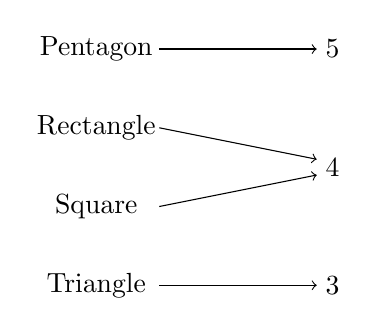
\begin{tikzpicture}
                \draw[align=right] (0, 0) node {Triangle};
                \draw[align=right] (0, 1) node {Square};
                \draw[align=right] (0, 2) node {Rectangle};
                \draw[align=right] (0, 3) node {Pentagon};
                
                \draw (3, 0.0) node {3};
                \draw (3, 1.5) node {4};
                \draw (3, 3.0) node {5};
                
                \draw [->] (0.8, 0) -- (2.8, 0.0);
                \draw [->] (0.8, 1) -- (2.8, 1.4);
                \draw [->] (0.8, 2) -- (2.8, 1.6);
                \draw [->] (0.8, 3) -- (2.8, 3.0);
            \end{tikzpicture}
            \caption{Digraph Relationship Between Polygons and the Number of Sides.}
            \label{fig:RelationshipBetweenPolygonsAndSides}
        \end{figure}
        
        Giving our relation between A and B the symbol $A \sim B$, we can also put them in a Cayley Predicate Table:
        
        \begin{table}[ht]
            \centering
            \begin{tabular}{|c|c|c|c|c|}
                \hline
                \multicolumn{2}{|c|}{\multirow{2}{*}{$A \sim B$}} & \multicolumn{3}{c|}{B} \\ \cline{3-5} 
                \multicolumn{2}{|c|}{} & 5 & 4 & 3 \\ \hline
                \multirow{4}{*}{A} & Pentagon & \cmark & \xmark & \xmark \\ \cline{2-5} 
                 & Rectangle & \xmark & \cmark & \xmark \\ \cline{2-5} 
                 & Square & \xmark & \cmark & \xmark \\ \cline{2-5} 
                 & Triangle & \xmark & \xmark & \cmark \\ \hline
            \end{tabular}
            \caption{Cayley Predicate Table of Relation Between Polynomials and Sides.}
            \label{tab:CayleyPredicateTableRelationPolynomialsSides}
        \end{table}
        
        Note from both table and digraph that $A \sim B \neq B \sim A$. In other words, it is not commutative, but we WILL discuss associativity.
        
        Discuss composition through ``matrix multiplication''. Discuss different symbolic ways to represent relations.
        
        You can notice that by looking at the Cayley Predicate Table that the checkmark (\cmark) is found exactly once per row of A. This is equivalent to saying that, on the diagraph, that there is exactly one arrow coming from each object of the shapes set.
        
        \begin{definition}
            A left-unique 
        \end{definition}
        
        A function in pure mathematics is not a function in computer science, despite that computer science is an offshoot of mathematcics (around the foundations of mathematics). The context of the word function changes in computer science to include side-effects, let's start with state and then go to sessions.
    
        Unary relations are set comprehensions
        \begin{section}{Function-Like Relations}
        \end{section}
        
        \begin{section}{Order-like Relations}
        
        \end{section}
        
        \begin{section}{Equivalence Relations}
        \end{section}
    \end{chapter}
    \begin{chapter}{Counting and Combinatorics}
        \begin{section}{adsf}
            \begin{subsection}{Relationships on the Boolean Algebra}
                \begin{align*}
                    |A \cap B| \leq |A| \quad  \textrm{and} \quad  |A \cap B| \leq |B|
                \end{align*}
                
                This is directly related to the fact that:
                \begin{align*}
                    X \subseteq Y \implies |X| \leq |Y|
                \end{align*}
                
                And this connection between these two, as important as it is, will be more thoroughly described later.
            \end{subsection}
            \begin{subsection}{Addition and the Disjoint Union}
            $$
                |A \sqcup B| = |A| + |B|
            $$
            \end{subsection}
            \begin{subsection}{Multiplication and the Cartesian Product}
            $$
                |A \times B| = |A| \times |B|
            $$
            \end{subsection}
            \begin{subsection}{Functions and Exponentials}
            $$
                |A \to B| = |B|^{|A|}
            $$
            \end{subsection}
            \begin{subsection}{Powerset as a Function}
            $$
                |\mathcal{P}(X)| = | X \to \mathbb{B} | = 2^{|X|}
            $$
            \end{subsection}
            \begin{subsection}{Permutations}
                Number of permutations = number of total orders ($|A|! = n!$)
            \end{subsection}
        \end{section}
    \end{chapter}
    \begin{chapter}{Probability Theory as a Logic}
    \end{chapter}
\end{part}
\begin{part}{Relations}
    \begin{chapter}{Binary Relations}
        \begin{section}{Heterogenous and Homogeneous Relations}
            Homogeneous means same-type, and heterogenous means different-type. In this regard, 
            
            Oftentimes, mathematically, we don't have specific words that mean possibly one and possibly the other. This is important, because a heterogenous relation can be homogenous too. The phrase non-homogenous specifically refers to a relation that must have different types.
        \end{section}
        
        \begin{section}{Heytingness}
            Make binary relation as ``included subsets'' ($R \in U\times V$) to a functional predicate for inclusion ($R : U \times V \to \mathbb{B}$) and that corresponds to ($R:U\to V \to \mathbb{B}$).
        \end{section}
        
        \begin{section}{asdf}
        \end{section}
    \end{chapter}
    
    \begin{chapter}{n-ary Relations}
    
    \end{chapter}
    
    \begin{chapter}{Relation Algebra}
    
    \end{chapter}
    
    \begin{chapter}{Other}
        A filter is a unary relation (can be useful as base-case in inductive arguments)
        
        A unary relation is a filter on a set (a subset)
        
        There are only 2 nullary relations: always holding and never holding
        
        A binary relation is a subset of the cartesian product
        
        A ternary relation requires an ordered n-tuple, since cartesian products are not associative. However, ((a, b), c) is also valid for discussion.
        
        
    \end{chapter}
\end{part}  
\begin{part}{Lambdas and Type Theory}
    \begin{chapter}{Lambdas and Combinators}
        Given our definition of functions in mathematics, we can define the truth-values of true and false as a choice. (describe by sentences and if/then).
        
        Then, we can define functions that allow us to select the first or the second part of the sentence:
        
        \begin{lstlisting}[language=Lambda]
            T x y = x
            F x y = y
        \end{lstlisting}
        
        \begin{lstlisting}[language=Lambda]
fix fib : int -> int.
  lambda n : int.
    if (n < 2) then n$^2$
    else (fib (n-1)) (fib (n-2))
\end{lstlisting}
        
        Then, the T function selects the first value, and the F function selects the second. It could just as well be called first and second, but we will define those later for a different purpose, and it will make less sense that this has anything to do with logic.
        
        Now, binding variables, in a way similar to quantifiers, we can define functions using lambdas, we will start with a function called the identify function, that gives you whatever you put in:
        
        \begin{lstlisting}[language=Lambda]
            I x = x
            I = lambda x.x
        \end{lstlisting}
        
        That is to say that the function I (again, standing for identity) is a function that takes a parameter x and returns that same argument.
        
        You will notice that instead of a symbol indicating set membership ($\in$), we separate the variable binding from the expression with the period.
        
        It may seem silly at first to have an alternative way to define a function, but the important thing is that we are not always interested in naming all of our functions. However, that's not the only benefit, the next benefit will come about as we keep talking.
        
        For now, let's define our true and false functions from before, rewriting them into lambda terms:
        
        \begin{lstlisting}[language=Lambda]
            T x y = x      T = lambda x.(lambda y.x)
            F x y = y      F = lambda x.(lambda y.y)
        \end{lstlisting}
        
        Now, again, this looks like it's creating more work, and if the goal was to express things with the least number of symbols possible, then we'd be failing. Instead. we are attempting to construct something, and the ideas will become more clear as we begin to make use of it.
        
        To apply an argument to a function looks like the following:
        
        \begin{lstlisting}[language=Lambda]
            T 3 5 = lambda x.(lambda y.x) 3 5
            T 3 5 =     (lambda y.3)   5
            T 3 5 =          3
        \end{lstlisting}
        
        The first action for application is to substitute x (the first parameter) with 3 everywhere it is used (which just so happens to be inside the parentheses). The second action is to substitute y with 5 everywhere y is found (which is not found anywhere.
        
        First things first, I want to talk about more standard order of operation (or probably more specific, ``order of interpretation'' in this case). Lambda abstractions are interpreted as right-associative, meaning that the definitions above are equivalent to:
        
        \begin{lstlisting}[language=Lambda]
            T = lambda x . lambda y . x
            F = lambda x . lambda y . y
        \end{lstlisting}
        
        \todo{discuss how this introduces us to functions that return functions}
        \todo{discuss the equivalence of this to the tuple form}
        
        Now, regarding the other operators that we'd expect from a Boolean data type, we'd expect to be able to interpret logical negation (NOT). In this case, if we logically negate the value, we swap T with F (and vice versa), which is equivalent to swapping which of the two values are selected. For instance, we'd expect the following:
        
        \begin{lstlisting}[language=Lambda]
            NOT T x y = y
            NOT F x y = x
        \end{lstlisting}
        
        So, a way that we could do this is to swap x and y:
        
        \begin{lstlisting}[language=Lambda]
            NOT p x y = p y x
        \end{lstlisting}
        
        If we used the same parameters as before, accepting T as the function that would be used:
        
        \begin{lstlisting}[language=Lambda]
            NOT T 3 5 = T 5 3
                      =   5
        \end{lstlisting}
        
        Notice that we can demonstrate the following:
        
        \begin{lstlisting}[language=Lambda]
            NOT T x y = T y x = y
                      = F x y = y
                
            NOT F x y = F y x = x
                      = T x y = x
        \end{lstlisting}
        
        So, we can say that applying NOT to T and F would give the same computed results as:
        \begin{lstlisting}[language=Lambda]
            NOT T = F
            NOT F = T
        \end{lstlisting}
        
        
    \end{chapter}
    
    \begin{chapter}{Types}
        \begin{section}{As a Pseudocomplemented Lattice}
            We discussed how function types act like the implication of a logic. Referring back to Order Theory, we also discussed Heyting Algebras and Pseudocomplements, and how the great thing about having a bounded semilattice was that we could generate a pseudocomplement from the bound.
        
            We assume that the upper bound is off limits in order to avoid Russell's Paradox on Types. However, we can attempt to find a lower-bound and use that instead. We need something that no type can be less than. Our first guess may be the unit type, but that still may not be the best type.
        
            Remember that a unit type can be passed to a function, and it can be returned from a function and then used. Imagine instead a type that cannot be constructed, and therefore it cannot return. We will call this type ``absurdity'' and it will be the bottom-element. This also means that we will often refer to it as the bottom type, and we will give it the symbol $\bot$.
        
            Therefore, we can also define our pseudocomplement (our negation) as a function that returns the bottom type: $A \to \bot$. Effectively, returning $\bot$ would be evidence that the program cannot compile (i.e. our proof fails). However, some programs are required to run forever, and so there may be situations where not returning is the correct behavior.
        
            With that out of the way, let's discuss the other property of a Heyting Algebra, that a monoid exists such that $c\wedge a \leq b \iff c \leq a \to b$. With the understanding that the $\leq$ actually means $\to$, we are looking for what meaning of $\wedge$ causes $c\wedge a \to b \iff c \to a \to b$.
        
            We have discussed previously that, when working with functions, we can call a function by $(A \times B) \to C$ or we can call it as $A \to (B \to C)$. This cartesian product is precisely the $\wedge$ we are looking for.
        
            This means that we have all the connections between the following:
            \begin{itemize}
                \item Boolean Logic (Heyting Algebras) -- $[(A\ \wedge\ B) \implies C] \iff [A \implies (B \implies C)]$
                \item Algebra -- $(c^{b})^{a} = c^{ba}$
                \item Type Theory / Functions -- $(A\times B) \to C \iff A \to (B \to C)$
                \item Category Theory -- $Hom(A \otimes B, C) = Hom(A, B \Rightarrow C)$
            \end{itemize}
        \end{section}
        \begin{section}{The Coproduct}
            We have defined the product in Type Theory now, and as we have stated, when there is a product, there is a coproduct in the opposite category. Well, we're going to skip the full categorical dual and continue discussing the relationships with the Heyting Algebra from before.
            
            Remember that, algebraically, when we have an exponential, we get the property that $(c^a)(c^b) = c^{a + b}$. It so happens that in logic, this also takes the same form that the join has: $(a \implies c) \wedge (b\implies c) \iff (a \vee b) \implies c$.
            
            So, we are looking for how to interpret $(A \to C) \times (B \to C)$, which are 2 functions, that allow us to get a type $C$ based on whether the input is $A$ or the input is $B$. In this regard, it's a choice between the inputs A and B. This has some characteristics similar to our disjoint union from set theory.
            
            We turn a proof of $A + B$ into a proof of $A$ or a proof of $B$, either of which allows us to get to $C$.
            
            In fact, we have a very perfect example of such a disjoint union available at hand:
            $$
                \mathbb{B} = T \vert F
            $$
            
            Where the ($\vert$) symbol means ``select between'', and being that T is a unit type (1), and F is also a unit type (1), then $\mathbb{B} = 1 + 1$ is sometimes denoted $2$.
        \end{section}
        \begin{section}{Peano Again}
            Now we are in a position to start defining Peano Arithmetic in Type Theory instead of plain ole Lambda Calculus. For that, we get the following:
            
            \begin{lstlisting}[language=Lambda]
                Nat = Z | S Nat
            \end{lstlisting}
            
            That is, we have the Natural Numbers defined as something that starts with zero (Z) and allows us to select a successor function (S) that takes a Natural Number as an input.
        \end{section}
    \end{chapter}
\end{part}

%----------------------------------------------------------------------------------------
%	CHAPTER 1
%----------------------------------------------------------------------------------------

\chapterimage{head2.png} % Chapter heading image

\chapter{Introduction}

\section{Motivation}\index{Motivation}
This book is a high-speed walk through the core mathematics and usages for various applications within science and engineering. It does not serve to teach proofs, or instruct on why the information contained herein works the way that it does, but instead serves to move straight to the heart of application.

The point of this book is to treat everything as computation. We will study arithmetic computations, algebraic computations, infinitesimal calculus, a calculus of sets, probability theory, statistics, etc. Until we have thoroughly gone through many of the most industry useful methodology.

The problem with this book is that it will make mathematics look as if it is about manipulating symbols in kind of ``mathematical language''. The duty and work of mathematicians was to create a system where it was possible that such symbolic manipulation is possible.

Worse yet, it allows one to forget that mathematicians are actively busy coming up with new things all the time. However, it's not the goal of this book to convince the reader of that. There are additional books in the series that are tuned to explaining just how we got where we are, and where we are going.

\chapter{Algebra/Working with Expressions}
The biggest difference between arithmetic and algebra is that arithmetic was interested in working with values and performing calculations on them. Algebraic manipulation is very effective, because there are plenty of things that can be put into an algebraic context, and then manipulated the way that we manipulate algebraic expressions.
\section{Expressions}
\begin{definition}{Expression}
A mathematical expression is a well-formed collection of symbols arranged according to rules called \textbf{syntax}.
\end{definition}

The symbols may represent operations, constants, variables, functions, brackets, etc. The brackets typically explicitly give the order of operations for the expression. When the symbols are omitted, a standard order of operations are accepted.

\section{Order of operations}
In order to understand the order of operations, it's important to start with the natural numbers.

\begin{remark}
    Natural numbers are the \emph{only} type of object where multiplication is repeated addition, and where exponentiation is repeated multiplication.
\end{remark}

This is only a means of remembering the order of operation, and is not directly a reason for how the order of operations became a commonly used standard. However, the definition, going into addition, multiplication, and exponentiation separate these operations into the following levels:

\begin{tabular}{|l|l|l|l|} \hline
Level & Action & Inverse Action \\ \hline
1 & Addition & Subtraction \\ \hline
2 & Multiplication & Division \\ \hline
3 & Exponentiation & \\ \hline
4 & Function Application & \\ \hline
5 & Brackets & \\ \hline
\end{tabular}

Therefore, if one gets the following expression, where $x=5$:

\begin{equation}
2(x-1)^3+\log(5+x)=0
\end{equation}

One works left-to-right, but starts with the highest level expressions first:

\begin{equation}
\begin{aligned}
2(5-1)^3+\log(5+5)& = 0 & \textsf{Expression with Substitution} \\
2(4)^3+\log(10)&=0 &\textsf{Brackets} \\
2(4)^3+1&=0&\textsf{Function Application} \\
2(64)+1&=0&\textsf{Exponentiation} \\
128+1&=0&\textsf{Multiplication} \\
129&=0&\textsf{Addition}
\end{aligned}
\end{equation}

\section{How to look at algebra}
For equations, we have the rule that, for any expression $x=y$ and any function ``f'':


Demonstrate to reader how this next equation is a consequence of equivalence classes...
\begin{equation}
x=y \Leftrightarrow f(x)=f(y)
\end{equation}

\part{Topics}
Foundational parts
\begin{itemize}
    \item Categories (logic and order)
    \item Model Theory (sets, types, etc.)
    \item Algebraic Theories (axiomatic definitions and symbolic manipulations through orders)
    \item Topology (including calculus)
\end{itemize}


\begin{itemize}
    \item The different meanings of equality: isomorphism vs identity
    \item Multiplication and addition as more fundamental than division or subtraction, with the exception of how subtraction is actually a distance function
    \url{https://www.quora.com/Do-we-need-division-and-subtraction-as-separate-operations-when-division-can-be-written-as-a-factor-with-the-exponent-of-1-and-subtraction-of-a-term-as-an-addition-of-the-negative-term-a-div-b-a-cdot-frac-1-b-a-b-a/answer/Nicholas-Cooper-8}
    
    \item That imaginary numbers are as imaginary as real numbers:
    \url{https://www.quora.com/Are-all-numbers-really-imaginary-numbers-How-are-numbers-real/answer/Nicholas-Cooper-8}
    \url{https://www.quora.com/What-real-world-phenomena-can-be-quantified-with-imaginary-numbers/answer/Nicholas-Cooper-8}
    
    \item The truth about measurements
    \url{https://www.quora.com/A-scalar-quantity-can-t-be-negative-because-it-only-has-magnitude-but-no-direction-but-why-can-temperature-can-be-negative/answer/Nicholas-Cooper-8}
    
    
\end{itemize}


%----------------------------------------------------------------------------------------
%	CHAPTER 3
%----------------------------------------------------------------------------------------
\printglossaries
\end{document}

\end{part}

\part{Mathematical Introduction to Philosophy}
%----------------------------------------------------------------------------------------
%	TABLE OF CONTENTS
%----------------------------------------------------------------------------------------

\chapterimage{head1.png} % Table of contents heading imag

%\cleardoublepage % Forces the first chapter to start on an odd page so it's on the right

\pagestyle{fancy} % Print headers again

Every symbol used in mathematics is like a pronoun is in natural language. When I say ``Cameron gave away his guitar'', you know that the word ``his'' is in reference to Cameron through context. Oftentimes, we are telling you want we want each variable, operator, and symbol to mean, but oftentimes, you will have to recognize the symbols from previous work.


\begin{chapter}{Introduction to Philosophy}
    No book that mentions philosophy is complete without describing those things that are intended, or valued as goals from the book, or in corporate speak a ``vision'' for the book. This is why this book does not have a formal introduction, but finds an introduction in this section, serving to introduce the importance of formalizing goals when doing work:
        
    \begin{section}{The Intended Value of this Book}
        This is a mathematics book, and the goal of this book is to teach mathematics. However, there are many books which aim to teach mathematics, but the author feels as if there is much missing in the way of:
            
        \begin{itemize}
            \setlength{\itemsep}{6pt}
            \setlength{\parskip}{12pt}
                
            \item \textbf{Intuitions} for the concepts being taught are not commonly taught because our intuitions can often lead us astray. Oftentimes, when we teach analogies, people assume the analogies are more real than analogous, and get angry and upset when the analogies fall apart. Therefore, a long discussion must be had to explain that an analogy doesn't necessarily mean something is equivalent.
     
            \item \textbf{Examples and motivations} of the concepts being used by people. This does not mean that every example needs to be something that is used by everyone, on a daily basis. Mathematics is often argued to be independent from the physical world, and despite the truth in that, the mathematicians who discover these things are not independent of the physical world, and so the physical world still informs the mathematician, and the learner.
               
            \item Because we will focus on examples and motivation from things in the physical world, we will also add \textbf{computer programming} to our learning curriculum, building up to it, nearly from the beginning. This will be a help and a hindrance, because computer literacy and knowledge of how to set up programming environments is not a focus of the lesson plans here. In fact, we should learn what the mathematical concept of a computer is, which is not necessarily the physical thing that this book was written on, but relates to it to a very strong degree.
                
            \item Along the line of the focus on examples, we will collect \textbf{interpretations} of mathematics as it is discussed, and disseminate those interpretations as best possible.
                
            \item Furthermore, the most important thing we will do is to connect various areas of mathematics, so that intuitions from one area will carry over to the other areas, and so will the proofs. Due to this, we may prove some theorems in more than one way in this book, so that the connections can be understood, and to help demonstrate what a theorem really is.
        \end{itemize}
            
        However, the additional focus on the things listed above does not imply that this book can avoid any of the items below, and must be discussed in balance, and with sufficient detail with the following: 
            
        \begin{itemize}
            \setlength{\itemsep}{6pt}
            \setlength{\parskip}{12pt}
                
            \item Formal definitions and descriptions of the concepts, including axiomatic definitions for mathematical structures
                
            \item Various constructions of mathematical structures when possible
                
            \item Formal reasoning for the properties of mathematical structures
        \end{itemize}
            
        You'll notice that these 3 all focus on mathematical structures, which may seem like a foreign concept right now. However, we will provide some heightened understanding of what a mathematical structure is by the end of this book.
            
        The intended reader of this book is adults, and in that respect, it is andragogy (the study of teaching adults), not pedagogy (the study of teaching children). It assumes certain concepts are already understood (like an intuitive feel for the number 250, and of place-value in general); however, it is the author's opinion that the order of subject matter given in this book is approximately the best order to teach children as well, given the mathematical subject matter available as of the year 2020.
    \end{section}
        
    \begin{section}{Motivation to Learn and a Warning to Learn it Well}
        \begin{subsection}{Knowledge is One Source of Strength}
            \begin{quote}{Edward Teller}
                The science of today is the technology of tomorrow.
            \end{quote}
            
            \begin{quote}{Chinese Proverb}
                If your mind is strong, all difficult things will become easy. If your mind is weak, all easy things will become difficult.
            \end{quote}
                
            Since we are still talking about philosophy, another good argument to learn philosophy, and to learn it well, is to build a strong mind through careful analysis of: your values, your own value, what makes you strong, and how you come to understand the world around you.
                
            However, the journey through these analyses are usually very personal. The last one, ``how you come to understand the world around you'' is the only one that this book intends to address in great detail, but being a mathematical book, and not a science book, it's actually less about understanding the physical world, and more about understanding what intuitions are actually happening in your own mind.
                
            We add mathematics to this study, because we realize what it brings to our society, as far as strength goes, by giving us these glimpses into the role that our intuitions have regarding how we interpret the world around us, and how those intuitions sometimes fail, and how often they actually succeed.
                
            The role of mathematics for our society is usually at one end of the chain of information that occurs between the various STEM-based subjects:
                
            \begin{figure}[ht]
                \centering
                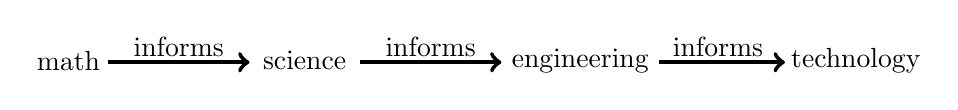
\begin{tikzpicture}
                    \node [align=center] at (0.0, 0.02){math};
                    \draw [ultra thick, ->] (0.5, 0) -- (2.3, 0);
                    \node [align=center] at (1.4, 0.2){informs};
                    \node [align=center] at (3.0, 0.02){science};
                    \draw [ultra thick, ->] (3.7, 0) -- (5.5, 0);
                    \node [align=center] at (4.6, 0.2){informs};
                    \node [align=center] at (6.5, 0.02){engineering};
                    \draw [ultra thick, ->] (7.5, 0) -- (9.1, 0);
                    \node [align=center] at (8.25, 0.2){informs};
                    \node [align=center] at (10, 0.02){technology};
                \end{tikzpicture}
            \end{figure}
                
            However, you'll also find that philosophy informs all of these, and is informed by all of these. The creative arts, like philosophy, is informed by all 4 of these, but tends towards informing only engineering and technology.
                
            This does not mean that mathematics and science is not creative, but it's often misunderstood that because mathematics is so rational, that it's not creative. It takes a lot of creative thinking and intuition, along with rational thought, in order to come up with mathematical proofs, and it is for this reason, and the connections to other fields, that creative arts is a necessary endeavour for anyone learning STEM.
                
            In fact, this is precisely the argument for STEAM.
                
            It must be stated more clearly, because the previous statement may not be clear enough: creative thinking, intuition, and rational thinking are \textbf{all} required for work in each of these fields of study, in concert with each other. Rational thinking does not promote mathematics and science alone. Intuitional thinking will almost certainly lead to falsehoods in these fields, if not matched with rational thinking.
                
            In this sense, creative thinking can be seen to be exploration, finding solution-after-solution, intuitive thinking can be seen to point the creative thinking along, but the rational thinking is the filter that finds the solutions that actually work.
                
            So, you will benefit all of these parts of your mind, including the part of you that is disciplined and builds grit. This will happen by mere practice and use, much like a muscle being used over-and-over getting bigger, and capable of handling more.
                
            Mathematics and the sciences change how you look at the world around you, but it doesn't make you a better person.
        \end{subsection}
        
        \begin{subsection}{The Danger in Strength}
            Philosophy has a long history of beneficial usage and of dangerous misuse. Philosophy may be the most important, but the most dangerous subject matter that a mind can consume. Philosophy has been used to free people as well as enslave people. The philosophical concept of moral or ethical \emph{justification} has been used both to protect and to kill.
            
            In effect, every argument about whether or not human beings are ready for a specific technology is actually a question of whether or not human beings are philosophically mature enough, and is captured in the following quotes:
            
            \begin{quote}{Jason Silva}
                Technology is, of course, a double-edged sword. Fire can cook our food but also burn us.
            \end{quote}
            
            \begin{quote}{Christian Lous Lange}
                Technology is a useful servant, but a dangerous master.
            \end{quote}
            
            \begin{quote}{B. F. Skinner}
                The real problem is not whether machines think, but whether people do.
            \end{quote}
            
            Replace ``technology'' with ``philosophy'' in the first two quotes, and you may begin to understand what it is that I'm claiming. Other quotes are a bit more direct:
            
            \begin{quote}{Martin Luther King, Jr}
                Nothing in all the world is more dangerous than sincere ignorance and conscientious stupidity.
            \end{quote}
            
            \begin{quote}{George Bernard Shaw}
                Beware false knowledge; it is more dangerous than ignorance
            \end{quote}
            
            \begin{quote}{Confucius}
                Real knowledge is to know the extent of one’s ignorance
            \end{quote}
            
            Oftentimes, it is exactly those strengths that serve as one's weaknesses, but that is not to say that having a strength necessarily creates weakness in that area. It benefits us to understand how strengths become weaknesses. 
    
            Philosophy, like technology, is good or bad, depending on how it's used, and depending on how well it's understood, and based on what principles one chooses to work from.
                
            In fact, the call-to-action I give each of you, before you start this endeavour is:
            \begin{itemize}
                \item Use your observations and experiences to help you understand your world
                    
                \item Uproot misperceptions and misunderstandings that come from a partial understanding of the first
                    
                \item Apply your understanding of the world to better your world and the world of others, as you see fit
            \end{itemize}
        \end{subsection}
        
        \begin{samepage}
            \begin{subsection}{Perceptions and Misperceptions of Philosophy, Mathematics, and Science}
                There are multiple misperceptions of about various fields of study, such as:
                \begin{itemize}
                    \item Mathematics
                    \begin{itemize}
                        \item It's not a creative field
                        \item It's the study of numbers
                        \item It's already finished (there's no new math to be had)
                        \item There are no jobs for mathematicians
                    \end{itemize}
                    
                    \item Science
                    \begin{itemize}
                        \item It's done by elite people who have no connection to reality
                        \item It's a collection of statements that are considered ``the truth''
                        \item It doesn't help ``real people''
                    \end{itemize}
                    
                    \item Software Development
                    \begin{itemize}
                        \item It's all copy-and-paste
                        \item Computers will be programming themselves soon
                        \item It's an easy desk-job with little pressure
                    \end{itemize}
                        
                    \item Economics
                    \begin{itemize}
                        \item It's the study of money
                        \item It's all psychology (which contradicts the first claim)
                    \end{itemize}
                \end{itemize}
            \end{subsection}
        \end{samepage}
            
        All of these claims are caricatures of the fields of study, or of the people who do work in those fields, and are not just oversimplifications, but are outright wrong if one were to actually follow these people around.
            
        Much the same misrepresentation occurs in all fields of study and all fields of work. These misrepresentations continue throughout the centuries as populism attempts to change the view of these subjects.
            
        The history of this populism is understood, because in history, fields such as these could only be achieved by the educated and the rich, and those people would not understand those who worked with their hands. Therefore, a schism occurred between those who used their minds, and those who used their hands, based on a classism that is not yet resolved.
            
        A shift has been occurring over the last few centuries though, especially as education has become more universal, allowing people to spend part of their lives in service, part of their lives in manual labor, part of their lives studying, and part of their lives working with their minds, and it's not certain that a person in any particular job has any particular experience.
            
        In this regard, philosophy has always been misrepresented, and you may hear things like:
        \begin{enumerate}
            \item Philosophy, like mathematics, has been completed, or it has produced all of the results and discoveries that it can
                
            \item Philosophy is useless, ungrounded, and a waste of a person's education
                
            \item Philosophy is nebulous, vague, and done by people who are out-of-touch with the real-world
                
            \item Philosophy opposes, is not supported of, or is somehow separate from science
        \end{enumerate}
            
        Nothing could be further from the truth on all of these grounds. Mathematics, and philosophy, are coming up with new discoveries all the time, and including applications to previous discoveries. Philosophy, especially the interest of how we come to know things, forms the basis for both mathematics and the sciences.
    \end{section}
    
    \begin{section}{What is Philosophy, and Why Should We Care?}
        Philosophy is typically introduced by discussing what it means, and where it comes from. We focus so much on the Greek philosophy, but philosophy, mathematics, and science has been growing in all cultures for millennia, and can be found as early trial versions of these subjects in ancient books all over the world.
            
        The word ``philosophy'' is a word from ancient Greek φιλοσοφία (\emph{philosophía}), which has 2 roots:
        \begin{itemize}
            \item φίλος (phílos meaning “loving”)
            \item σοφία (sophía meaning “wisdom”)
        \end{itemize}
            
        However, that only scratches the surface, and tends to lead to the conclusion that “philosophy is in every query”. Although this is technically true, it does little to give anyone any clue to what philosophers actually do, and why it’s important.
            
        In some ways, philosophy is the process of exploring one’s thoughts, asking ourselves, “why do I think this way?”
            
        Specifically, philosophers have certain question that all philosophy branches out from:
            
        \begin{figure}[ht]
            \centering
            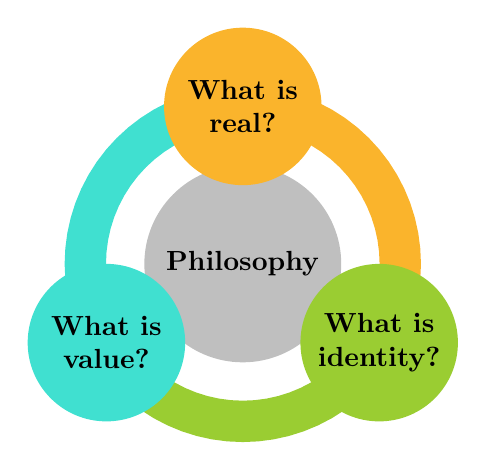
\begin{tikzpicture}
                \fill [lightgray]   (0,0) circle (12.5mm);
                \node [align=center] at (0, 0) {\textbf{Philosophy}};
                \draw [Dandelion,line width=5.25mm,domain=-30:90] plot ({2*cos(\x)},     {2*sin(\x)});
                \draw [YellowGreen,line width=5.25mm,domain=210:330] plot ({2*cos(\x)},     {2*sin(\x)});
                \draw [Turquoise,line width=5.25mm,domain=90:210] plot ({2*cos(\x)},     {2*sin(\x)});
                \fill [Dandelion] (0,2) circle (10mm);
                \fill [YellowGreen] ( 1.732,-1) circle (10mm);
                \fill [Turquoise]   (-1.732,-1) circle (10mm);
                \node [align=center] at ( 0.000, 2) {\textbf{What is}\\\textbf{real?}};
                \node [align=center] at ( 1.732,-1) {\textbf{What is}\\\textbf{identity?}};
                \node [align=center] at (-1.732,-1) {\textbf{What is}\\\textbf{value?}};
            \end{tikzpicture}
            \caption{The 3 Proposed Root Questions of Philosophy.}
            \label{fig:ThreePhilosophicalQuestions}
        \end{figure}
            
        Here though, these 3 questions feed off of each other. For instance, 
        \begin{itemize}
            \item Is it possible to seek truth without asking what methods of truth-seeking that we value?
                
            \item If something exists (if it’s “real” or “true”), can we identify it?
                
            \item If we change something (identity) does it change value?
        \end{itemize}
            
        In fact, these three questions spawn multiple branches of study, some of which are considered philosophical in modern times still, others may appear, on the surface, as if they are something separate from philosophy.
            
        \begin{subsection}{What is Real?}
            Epistemology relates to the question, “How do we know what we know?”. The study     of epistemology has given us logic (forming the foundations of mathematics),     the Scientific Method (forming the foundations of science), and gives us     mechanisms for us to understand beliefs by asking:
                
            \begin{itemize}
                \item What does it mean to know something?
                \item Can anything be known for certain? 
                \item How much confidence can we have in something?
                \item What is the process that we come to know things?
                \item What does it mean to know things?
                \item What is a belief?
                \item Can we justify our beliefs? (\textbf{critical reasoning})
                \item What is the relationship between beliefs and knowledge?     (\textbf{doxastic logic})
            \end{itemize}
        \end{subsection}
            
        \begin{subsection}{What is Identity?}
            In philosophy, we talk about \textbf{discernibility}, which lets us ask, “if two things share all the same properties, are they the same thing?”. We use this in mathematics to present two things being equal. In science, we identify phenomena that interest us. In our lives, we discuss personal identity, social identity, and even discuss the human identity. In many ways, the philosophical focus on definitions and on meanings are directly related to identifying concepts, and coming to agreement on concepts, in order to help discuss.
                
            It leads us to questions like:
                
            \begin{itemize}
                \item What does it mean for two things to be the same, and does that change over time or based on the context?
                \item If I replace every component with an identity component, is it the same thing (Interchangeability and compatibility)?
                \item Are we the same person from one moment to the next?
                \item Is any object the same from one moment to the next?
                \item How do we relate to and do we identify with our city, our culture, and/or our nation?
                \item What does it mean when things are “almost alike” or similar? And do similar things share similar properties?
            \end{itemize}
        \end{subsection}
        \begin{subsection}{What is Value?}
            The notion of \textbf{value} or \textbf{worth} is also of central concern, as it allows us to compare two things. This is also of central concern in mathematics as it allows us to make statements about relationships between things. It is of concern in modern politics, when discussing the value of citizens and whether or not they feel valued. We discuss \textbf{aesthetics} as the study of those things that attract our senses. We discuss \textbf{ethics} through the value of actions. It leads us to questions like:
                
            \begin{itemize}
                \item What does it mean to compare two things?
                \item Why do things cost what they do?
                \item What do individuals value, and why?
                \item What do societies value, and why?
                \item Is something practical worth more than something else? What makes it practical?
                \item What is fairness and justice?
            \end{itemize}
        \end{subsection}
        \begin{subsection}{What is the Relationship Between Value and Identity?}
            When questions about both value and identity come together, we usually start to ask about purpose, and
            \begin{itemize}
                \item Is there a purpose to the existence of the universe? What is the purpose?
                \item Is there a purpose to my existence? What is the purpose? Do I create my own purpose?
                \item Am I a valued part of my community? Why or why not?
                \item What is fair when it comes to treatment of different people?
                \item How does interchangeability relate to comparison? If I interchange components for something newer, is it better?
            \end{itemize}
        \end{subsection}
        \begin{subsection}{What is the Relationship Between Value and Truth?}
            This is the intersection of the two questions that lead us to asking questions like:
            \begin{itemize}
                \item How do we value the various means of obtaining knowledge?
                \item How do people value methods of communicating knowledge and beliefs?
                \item Whose testimonies do we believe and why?
                \item Can there be an absolute, top-level truth, by which all other truths are measured?
                \item Can there be a best moral code, by which all other moral codes are measured?
            \end{itemize}
        \end{subsection}
        \begin{subsection}{What is the Relationship Between Identity and Truth?}
            Regarding identity and truth, we may get some interesting questions about ourselves and:
            \begin{itemize}
                \item What are we? (i.e. what makes us human, or what makes us different?)
                \item Where do we come from?
                \item Why does anything exist at all?
                \item How do we relate to our perceptions, and vice versa?
                \item What does it mean to “exist”?
                \item What does it mean to be “real”?
                \item What is reality?
                \item What is the mind?
            \end{itemize}
        \end{subsection}
        \begin{subsection}{What is the Relationship Between All 3?}
            Finally, we can consider all 3 together:
            \begin{itemize}
                \item Is there something bigger than us?
                \item What is out there, beyond what we can perceive?
                \item How did this universe come to exist? (\textbf{cosmology})
                \item What is the greatest possible mind? Must a creator exist? (\textbf{theology})
            \end{itemize}
        \end{subsection}
            
        \begin{subsection}{Categorizing the Questions into Branches}
            Many of these questions have been placed into various categories:
            \begin{itemize}
                \item That reason can be a source of knowledge (\textbf{rationalism}) allowed us to create logic, and logic continues to refine the foundations of mathematics (classically called, “the formal sciences”)
                    
                \item Critical thinking, using our senses as a source of knowledge (\textbf{empiricism}), building confidence through experimentation (\textbf{verificationism}), and filtering in only those things that we can derive from these sources (\textbf{positivism}) refines the scientific method, which gives us science (classically called, “the physical sciences”)
                
                \item Questions about value form the basis for \textbf{Value Theory}, and include subbranches like: ethics, aesthetics, and axiology (moving into application through economics and politics)
                    
                \item Questions about existence and reality form the basis of \textbf{Metaphysics}, and include subbranches like: theology, religion, and ontology 
                    
                \item Questions about how we do philosophy form the basis of \textbf{Metaphilosophy}
            \end{itemize}
        \end{subsection}
    \end{section}
    
    \begin{section}{Philosophical Discussions}
        So, you thought that this book was going to be about mathematics. Why, then, are we learning philosophy? Well, it turns out that philosophy is the parent of almost every subject studied in any formal education. 
            
        Given that we have asked about reality, science is a formal discipline of the philosophical position called empiricism, allowing us to enter into discussion about those areas of discussion that can be observed and measured with repeatable results. However, as positions go, science is limited to such discussions.
            
        Foremost, we are interested in mathematics in this book, but we will only really get there by discussing the roots of mathematics. Also, in order to understand it, we will do best when we can also link our study to various other areas as well. The most interesting part is how these things link.
            
        \begin{figure}[ht]
            \centering
            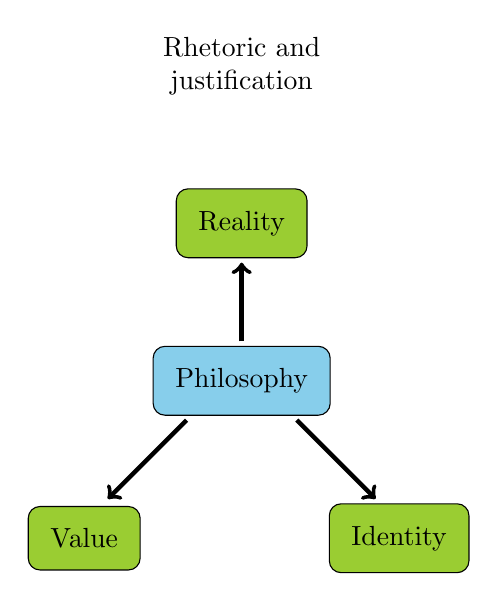
\begin{tikzpicture}
                \node [align=center,draw=black,fill=SkyBlue,thin,inner sep=8pt,rounded corners=.15cm] at (0.0, 0.0) {Philosophy};
                
                \node [align=center,draw=black,fill=YellowGreen,thin,inner sep=8pt,rounded corners=.15cm] at (0.0, 2.0) {Reality};
                
                \node [align=center] at (0.0, 4.0) {Rhetoric and\\justification};
                
                \node [align=center,draw=black,fill=YellowGreen,thin,inner sep=8pt,rounded corners=.15cm] at (-2, -2.0) {Value};
                
                \node [align=center,draw=black,fill=YellowGreen,thin,inner sep=8pt,rounded corners=.15cm] at ( 2, -2.0) {Identity};
                
                \draw [ultra thick, ->] ( 0.0, 0.5) -- (0.0, 1.5);
                \draw [ultra thick, ->] (-0.7,-0.5) -- (-1.7, -1.5);
                \draw [ultra thick, ->] ( 0.7,-0.5) -- ( 1.7, -1.5);
                %\node [align=center] at (0.0, 0.02){math};
                %\draw [ultra thick, ->] (0.5, 0) -- (2.3, 0);
                %\node [align=center] at (1.4, 0.2){informs};
                %\node [align=center] at (3.0, 0.02){science};
                %\draw [ultra thick, ->] (3.7, 0) -- (5.5, 0);
                %\node [align=center] at (4.6, 0.2){informs};
                %\node [align=center] at (6.5, 0.02){engineering};
                %\draw [ultra thick, ->] (7.5, 0) -- (9.1, 0);
                %%\node [align=center] at (8.25, 0.2){informs};
                %\node [align=center] at (10, 0.02){technology};
            \end{tikzpicture}
        \end{figure}
            
        \begin{figure}[H]
            \centering
            \includegraphics[scale=0.65]{PhilosophicalIntroduction/ConnectionsToPhilosophy.png}
            \caption{Connections of Various Fields to Philosophy.}
            \label{fig:ConnectionsToPhilosophy}
        \end{figure}
            
        \begin{subsection}{Rhetoric and Justifying Beliefs}
            It's important to understand that much of our mental sophistication revolves around explaining ourselves to others, whether that be in regards to giving them a mental image of what we have seen, explaining how something works, to justifying our reasons for doing something.
                
            Jonathan Haidt gave us the analogy of our minds being of a human rider on top of an elephant, whereas the rider is the rational mind, and the intuition is the elephant. We are so good at justifying our actions to others, that we often justify things we have done to ourselves, even when we know better (e.g. ``I can eat that whole chocolate cake, because I've done so well on my diet this week.'').
                
            Our written Greek philosophy seems to start with regards to \textbf{rhetoric}, as the ``art of discussion'', developing the communication skills to discuss philosophical positions.
                
            Rhetoric was often divided into:
            \begin{itemize}
                \item \textbf{Emotional} appeals, intended to speak directly to the mind's elephant. These appeals are often highly effective, if sometimes manipulative in their usage.
                    
                \item \textbf{Authoritative} appeals, intended to invoke the authority of the speaker, through their experience or due to their character-history of truthfulness.
                    
                \item \textbf{Rational} appeals, intended to speak directly to the rider of the elephant, who is capable of mapping out a direction for the elephant to travel, if the rider can ever get the elephant to listen.
            \end{itemize}
                
            We may be used to hearing the word rhetoric in political discussions (such as ``inflammatory rhetoric''), but oftentimes the person using the word doesn't mean it with the nuance of the philosophical meaning. Instead, philosophers would deem what politicians are doing \textbf{polemic}, which is emotional arguments intended to reduce confidence in and incite fear of an opponent.
                
            It should be obvious that mathematics and the sciences are filled with logical appeals, and as such, this book will be filled with them as well. However, it's also recognized that the intuition must be brought on board as well. 
                
            Finally, the authoritative appeals should be mostly unused in any discussion of mathematics. There is no for a teacher to use appeals to authority, saying things like ``it just works this way''. The only authoritative appeals will be the usage of already defined and commonly used standards for writing that may be brought up. However, even those should be backed with arguments for rational reasons why.
                
            \begin{subsubsection}{Some Definitions}
                
                \begin{definition}
                    An \textbf{interlocutor} is a person that is taking part in a dialog.
                \end{definition}
                    
                \begin{definition}
                    A \textbf{proposition} is a statement is possibly true or false.
                \end{definition}
                    
                \begin{definition}
                    A \textbf{premise} is a proposition for consideration, sometimes asserted as true by the interlocutor, and sometimes as a condition for the context of the argument.
                \end{definition}
                    
                \begin{definition}
                    A \textbf{conclusion} is a proposition that is the end result that the interlocutor reaches starting from the premises.
                \end{definition}
                    
                \begin{definition}
                    An \textbf{argument} is a series of propositions, structured such that the premises lead to a conclusion. Furthermore, a more general meaning of this word may be a process of reasoning.
                \end{definition}
                    
                \begin{definition}
                    A premise taken as a condition, usually in regards to an investigation is called a \textbf{hypothesis}.
                \end{definition}
                    
                \begin{definition}
                    A \textbf{philosophical position} is a collection of premises that an interlocutor is arguing from.
                        
                    It is often called a \textbf{philosophical theory}, which can cause confusion with the significantly different meanings taken by scientific theory and mathematical theory. 
                        
                    The everyday usage of the word ``theory'' is probably best identified as ``hypothesis''.
                        
                    Due to this confusion, the word position will be preferred in this book.
                \end{definition}
                    
                \begin{figure}[ht]
                    \centering
                    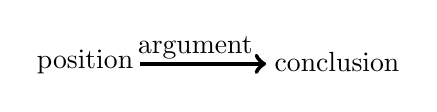
\begin{tikzpicture}
                        \node [align=right] at (0.0, 0.02){position};
                        \draw [ultra thick, ->] (0.7, 0) -- (2.3, 0);
                        \node [align=center] at (1.4, 0.2){argument};
                        \node [align=left] at (3.2, 0.02){conclusion};
                    \end{tikzpicture}
                    \caption{Relation between position (premises), argument, and conclusion}
                \end{figure}
                    
                \begin{definition}
                    For the sake of comparison, a \textbf{life stance} is a philosophical position that one takes, according to their worldview, which informs their beliefs, their thoughts, and their behavior.
                        
                    This is stated separately, since a life stance differs from a philosophical position.
                \end{definition}
                    
                \begin{definition}
                    A \textbf{Devil's Advocate} is a person that argues from a position that differs from their life stance, in order to better understand their own position, and the position of others.
                \end{definition}
                    
                \begin{definition}
                    \textbf{Skepticism} is the act of reserving belief for future evidence.
                \end{definition}
                
                \begin{definition}
                    \textbf{Belief revision} is the act of modifying one or more premises that make up a position, due to new evidence.
                \end{definition}
            \end{subsubsection}
            
            \begin{subsubsection}{What Forms a Worldview}
                At this point, I'm going to present what follows as a position, setting the rest of the book up for discussions on logical reasoning.
                    
                \begin{remark}
                    This position I am starting from, regarding worldviews, is not scientific, is not based on psychological evidence, and is likely just an approximation of how worldviews actually work.
                \end{remark}
                    
                \begin{figure}[ht]
                    \centering
                    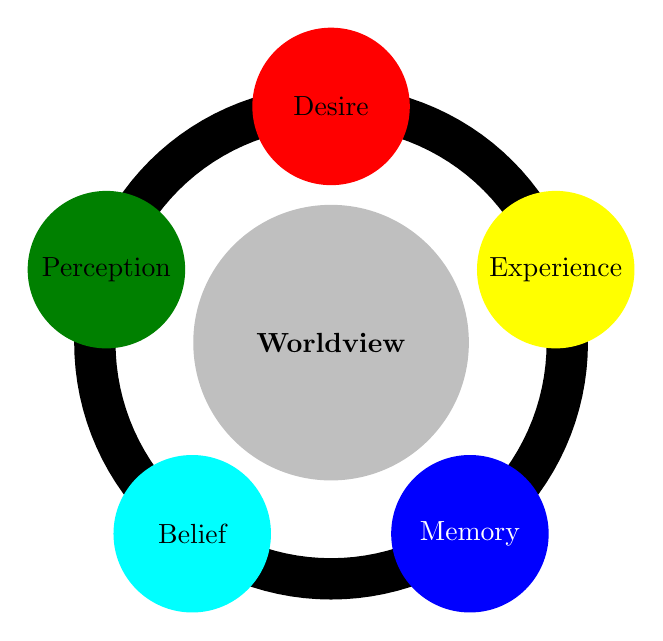
\begin{tikzpicture}
                        \fill [lightgray] (0,0) circle (1.75cm);
                        \node [align=center] at (0, 0) {\textbf{Worldview}};
                            
                        \draw [Black,line width=5.25mm,domain=90:162] plot ({3*cos(\x)}, {3*sin(\x)});
                        \draw [Black,line width=5.25mm,domain=162:234] plot ({3*cos(\x)}, {3*sin(\x)});
                        \draw [Black,line width=5.25mm,domain=234:306] plot ({3*cos(\x)}, {3*sin(\x)});
                        \draw [Black,line width=5.25mm,domain=306:378] plot ({3*cos(\x)}, {3*sin(\x)});
                        \draw [Black,line width=5.25mm,domain=378:450] plot ({3*cos(\x)}, {3*sin(\x)});
                            
                        \fill [Red]   ( 0.000000, 3.000000) circle (10mm);
                        \fill [Green] (-2.853170, 0.927051) circle (10mm);
                        \fill [Cyan]  (-1.763356,-2.427051) circle (10mm);
                        \fill [Blue]  ( 1.763356,-2.427051) circle (10mm);
                        \fill [Yellow]( 2.853170, 0.927051) circle (10mm);
                            
                        \node [align=center,text=black] at 
                        ( 0.000000, 3.000000) {Desire};
                        \node [align=center,text=black] at 
                        (-2.853170, 0.927051) {Perception};
                        \node [align=center,text=black] at 
                        (-1.763356,-2.427051) {Belief};
                        \node [align=center,text=white] at 
                        ( 1.763356,-2.427051) {Memory};
                        \node [align=center,text=black] at 
                        ( 2.853170, 0.927051) {Experience};
                    \end{tikzpicture}
                    \caption{Relation between position (premises), argument, and conclusion}
                \end{figure}
                    
                The first question someone may have looking at the components of a person's worldview that I listed is that experience, memory, and belief are all the same thing. However, my argument is that we experience all the time, but our beliefs color how we interpret the memories associated with those experiences.
                    
                In this sense, we reexperience things through our memory, but it doesn't mean that it feels the same each time.
                    
                It may seem strange that I put desire in with the rest of these, because it appears that the rest of these relate to knowledge, but that desire is completely unrelated. However, we already know that desires change how we perceive things, making us more or less perceptive of our failures or successes, or how other people act.
                    
                The point of all of this is to say that our memories are fallible, because they change. Our perceptions are fallible as well, and so, we cannot always trust our worldview.
            \end{subsubsection}
                
            \begin{subsubsection}{What Sources of Information do you Value?}
                In the discussion of rhetoric, we talked about 3 different types of arguments: emotional, authoritative, and rational.
                    
                However, these are only the methods of transference of information from one person to another, and misses an important source of information: experience.
                    
                We tend to regard experience as the most valued source of information, but as we discussed in regards to the worldview, our perceptions of experiences are often incomplete, and sometimes even wrong.
                    
                Most people, naturally value emotional, authoritative, experiential, intuitive, and rational information sources to some level or another, because we naturally recognize that there are failings with putting all of our trust in any one of them: emotions can sometimes be erratic, people sometimes lie, our perceptions often deceive us, our intuitions are often wrong, and we often don't have enough information to come to a rational conclusion.
                    
                However, there are things that we can do to refine when we use each, and what we can be said about each source of information.
                    
                Firstly, it's important to note that rational arguments begin as intuitive arguments. Humans have an intuitive ability to recognize cause-and-effect, allowing us to determine how things work, and often change how things work to our favor. This recognition of the pattern of cause-and-effect is what leads us to logic, and rational thinking is the disciplined use of this logic. 
                    
                In fact, the discipline is what separates intuition from rational thinking. We follow through with our intuitions to see if they fail.
                    
                Second, the relationship between emotions and intuition are also important. Purely rational thinking is devoid of creativity, can get stuck in analysis, and therefore absent problem solving ability. However, purely intuitive thinking cannot weed out those ideas that won't work, and will naturally try things that are not logically sound, usually wasting their own and other people's time.
                    
                First, let's get more detailed how these each operate as a source of information:
                \begin{itemize}
                        
                    \item Authoritative sources
                    \begin{itemize}
                        \item \textbf{Witnesses} can provide accounts of events
                        \item Parents and teachers often provide us tons of information
                    \end{itemize}
                    \item Experiential sources
                    \begin{itemize}
                        \item Your \textbf{senses} give you access to the world around you and are your connection to it
                        \item When your senses act together they create an \textbf{empirical} view of the world
                        \item This effectively places you as an authority over your own worldview
                        \item Demonstrations from other individuals can help communicate subject matter
                    \end{itemize}
                    \item Emotional and Intuitive sources
                    \begin{itemize}
                        \item Emotions can point us to how our intuitions react to specific experiences
                        \item Gut feelings can tell us things about our world, and are frequently part of our mental pattern-matching capabilities.
                        \item It is via these gut feelings that we are capable of walking, knowing where to place each foot as we move
                        \item The intuitive is unconscious, but quick to form conclusions
                    \end{itemize}
                    \item Rational sources
                    \begin{itemize}
                        \item We use logic and probability to determine whether or not something is possible
                        \item We use analogy to compare and contrast things that we know against things that we do not know
                    \end{itemize}
                \end{itemize}
                    
                We know that authorities can lie, and that witnesses can't always trust their memories. Likewise, we cannot always trust our senses, nor our memories. Our emotions and intuitions are often wrong. Also, we can misuse logic, probability, and analogy.
                    
                In seeking information that we can trust, it seems like we are out of luck, but through careful inspection, we can begin to clear out the mess.
                        
                Regarding rational and intuitive thought, if we learn how to properly use logic and to understand our own biases, we can balance intuition with rational thinking, by allowing intuition to come up with hypotheses, and cutting through the wrong ones via rational thought. We can learn how where rational thinking works, and how sometimes fails us.
                    
                Regarding experience, we can learn about our own psychology, and also through our biases, determine when we can trust our senses and our experiences. We can determine whether multiple memories working together with evidence can corroborate our hypotheses.
                    
                Regarding authorities, \textbf{Subject Matter Experts} are people who are experienced in a subject matter and have a record of insightful discussions, and as long as they have no motive to lie to us, information inside their area of expertise can be trusted.
                    
                From there, we can actually learn what authorities know, how they came to their conclusions, and come to conclusions ourselves via experience and rational thinking.
                    
                So, it's important to think about how and why you value the sources of information that you do, how and why they can fail you, and how to effectively work through them.
            \end{subsubsection}
                
            \begin{subsubsection}{Epistemology}
                The study of what we know and how we come to know it is called \textbf{epistemology}. It is extremely important in the realm of mathematics and the sciences to understand epistemology, 
            \end{subsubsection}
            \begin{subsubsection}{Rigorous Communication}
                Furthermore, most of this communication between experts requires that the words they use are well-understood. We have definitions for words that we use all the time, but often words in a particular \emph{subject matter} have explicit definitions which differ from how they are used in everyday speech.
                    
                Let's consider one of the most problematic words in use today. The word \textbf{theory} from the ancient Greek θεωρία (``theoria'') was contrasted to πρᾶξις (``praxis'' where we get the word ``practice''). The theory behind something was the contemplation regarding how an activity works, and the praxis was the act of doing it. Therefore, theory was used to improve the praxis, but praxis was used to improve the theory.
                    
                This contrasting terminology between the two is why we still have phrases like ``that's works in theory, but not in practice''. However, the meaning of theory in our everyday life is not necessarily how it is used elsewhere:
                    
                \begin{itemize}
                    \item \textbf{Theory (science)} -- a hypothesis which is confirmed by repeated and thorough experimental observation to provide reliable predictions
                    
                    \item \textbf{Theory (mathematics)} -- the collection of premises and conclusions related specific mathematical structures
                        
                    \item \textbf{Theory (philosophy)} -- the collections of premises and conclusions specific to an area of philosophical pursuit (also called a philosophical position).
                        
                    \item \textbf{Theory (everyday speech)} -- a proposed explanation serving as a hypothesis
                \end{itemize}
            \end{subsubsection}
                
                
        \end{subsection}
        \begin{subsection}{Ontology and the Mathematics of Identity, Equality, and Equivalence}
            Discernibility
            Distinguisibility
            Interchangeability
            Identical
                
            \begin{subsubsection}{Definitions}
                In every field of study, we have to be extremely careful what it is we mean when we say something, and aim to avoid
                    
                In mathematics, we often define something, to use in a context (a scope of discussion) and when we are done, we stop meaning it the same. In speech, we do this often with pronouns. For instance, ``Caleb left work. He wasn't feeling that well.''. We immediately know that `He' in the sentence refers to Caleb. In this case, with English, we didn't even specifically define that we'd use `He' this way.
            \end{subsubsection}
                
                
            \begin{subsubsection}{Isomorphisms}
                \begin{definition}
                    The word \textbf{isomorphism} has a formal definition that we will cover later in Category Theory. Philosophically, it can be thought best to first recognize that mathematical objects are conceptual, not physical, and we can argue only that two objects constructed exactly the same way (structural identity) are identical. However, as we have said, two objects can be constructed in 2 different ways and behave as if they are the same object. These objects then have interchangeability between them.
                    
                    An isomorphism focuses, not on identical constructions (what the objects ``are''), but on identical behaviors (what the objects ``do''), and more specifically, that they adhere to the same ``legal contracts'' we call axioms.
                    
                    The word isomorphism (iso- ``same'', -morphism ``form'') is an effective ``equality between types of things''. 
                \end{definition}
                
                An example would be the 2 identical definitions for the number 1:
                \begin{enumerate}
                    \item The natural number comes after 0
                    \item The unique natural number that allows us to multiply any number by itself and result in the same number
                \end{enumerate}
                
                Both of those definitions for 1 focus on what it does, but the first definition is closer to the actual construction of 1 than the second. The two definitions are isomorphic to each other.
                    
                Furthermore, we have the Univalence Axiom, which binds multiple mathematical fields together, in the same way that René Descartés bound algebra together with geometry when he noticed that we can put things on a grid. The proposal of the Univalence Axiom first observed that equivalence (structural identity) implies isomorphism(interchangeability), but the true observation was that an isomorphism was interchangeable with an equivalence.
                
                Now, that's not being fully honest, and yet it is at the same time. A good philosopher will think to themselves, ``you didn't use the word `equivalence' the same way in both of those sentences'', and that philosopher would be right.
                
                I started the discussion talking about identical constructions (what objects ``are''),and obviously, two things cannot be equivalent if they do not have identical constructions. However, equivalence doesn't have to mean identical constructions.Mathematicians often define equivalence based on interchangeability in the same sense as the following analogy:
                
                \begin{quote}
                    A ``Gizmo'' machine has a component called a ``doohickey''. If I can take the doohickey out and replace it with another doohickey, they are interchangeable. If I can replace the Gizmo with another Gizmo, and use the same doohickey in both, then the Gizmo itself is fungible (interchangeable with other things that use components). If any doohickey can go in any Gizmo, then the differences between each doohickey is indiscernible.
                \end{quote}
                
                So, we get an isomorphism between algebraic equations and geometry from Descartés. From Euler we'll see how trigonometry, calculus, and complex numbers relate. However, here we use this opportunity to note that there is an isomorphism between paths, logic,partial orders, computation (and computer science), and tons of things we may get to later, just from Vladimir Voevodsky's Univalence Axiom.
                
                Finally, I have mentioned Axioms as ``legal contracts for mathematical structures''.You may be asking, what structure do we assume Univalence for? We will eventually get into Category Theory, and that will help combine all the world of mathematics together for us.
                
                So, it helps to understand that equality has context, just as isomorphism has context, and we may discuss various types of equalities.
            \end{subsubsection}
                
            \begin{subsubsection}{Natural Numbers are not Non-negative Integers}
                Never does the distinction and non-distinction matter as much as how we teach the number classifications. We have probably been taught that we can identify integers as allowing for negative numbers, and that every natural numbers \textbf{is} an integer.
                    
                This notion of \textbf{is} refers to our isomorphism from earlier. We can construct integers, and we can construct natural numbers, and we will construct them later, but the statement ``\textbf{is}'' used above must be understood to mean that we can get an integer from a natural number, and take that same integer and find a natural number that matches it. That is what it means to ``be the same''.
            \end{subsubsection}
        \end{subsection}
    \end{section}
\end{chapter}
\chapter{Logical Deduction}
\section{Classical Logic}
Socrates tells us that Plato gave us 3 \gls{LawsOfThought} (paraphrased here, and using the notion of ``true'' as a value):
\begin{itemize}
\item \textbf{Law of Identity} –- For any statement P, P = P. This is to say that true is true, false is false, and this law basically defines a notion of equality for logic.
\item \textbf{Law of Non-Contradiction} –- No two contradictory statements can both be true. For instance, it cannot be that ``Humans are animals'' and ``Humans are not animals''.
\item \textbf{Law of the Excluded Middle} –- Everything must be either true or false.
\end{itemize}

There are also records of the Law of Non-Contradiction in the Indian Sutras, but the most well-known collection of these 3 laws is by Socrates.
Aristotle also gave us one more law, codified as the \textbf{syllogism}:
If we have the following two statements:
\begin{itemize}
\item If X then Y
\item X
\end{itemize}
Then we can conclude Y; and hence, justification in intuitionistic logic is interpreted as “reachability”, the ability to reach Y from X.

An example of a syllogism would be, “If it is raining in the open field, then the ground is getting wetter”, and “it is raining” giving us the result that “the ground is getting wetter”

Now, it may seem counterintuitive, but we cannot conclude the logical converse (swapping). In other words, we cannot use wet ground to conclude that it is raining, because sprinklers may be on, or the water hose running over the ground.

\todo{treat it like a path}
\chapter{Boolean Logic}
\section{The Boolean Domain}
We often talk about different structures in mathematics, starting with what possible values it can have. The \gls{BooleanDomain} is used to describe something that has 2 possible values, but also interpret
one value as \emph{true} and the other as \emph{false}.

Following the discussion of Classical Logic, the Boolean Domain represents the possible values that Classical Logic can have, since Classical Logic uses the Law of the Excluded Middle to claim that there
are only 2 possible values.

When we are working with the Boolean Domain, we call a possible element a \gls{bit}.
\subsection{Symbols for Elements}
There are numerous ways to represent the Boolean Domain, and some can be interpreted below:
\begin{table}[ht]
\centering
\begin{tabular}{|c|c|c|c|c|}
    \hline
    False & 0 & $\bot$ & F & \texttt{-}1 \\ \hline
    True  & 1 & $\top$ & T & \texttt{+}1 \\ \hline
\end{tabular}
\end{table}

Each has a use that makes more sense in some situations over others. In this book, we will typically use T and F as the 2 values used to describe \emph{true} and \emph{false} respectively, but here is how the others may be used:

\begin{itemize}
    \item 0 and 1 are used in computers, and represent values that mean that a circuit is enabled (1) or disabled (1). Of course, we can reverse the meaning of these two, but typically enabled and disabled are 1 and 0 respectively.
    
    \item $\bot$ and $\top$ are used to demonstrate that Boolean Logic is symmetrical, in a way that will be described later.
    
    \item \texttt{-}1 and \texttt{+}1 are used rarely to demonstrate how Boolean Logic can be viewed in a way similar to arithmetic.
\end{itemize}

\subsection{Symbols for the Domain Itself}

The symbol for the Boolean Domain itself is $\mathbb{B}$. The elements will be referred to as T and F. Therefore, we will later make frequent use of symbolic relations like the following:

$$
    \mathbb{B} = \{T, F\}
$$

Which means to say that the Boolean Domain ($\mathbb{B}$) is ($=$) the set of items with a true and false ($\{T, F\}$).

\section{Interpretation as Logical True and False}
To interpret the values T as having logical truth is to also say that T is more true than F is. It may at first seem like mathematics says a lot off obvious things, but sometimes it needs to be stated for other conclusions to be made.

With that interpretation in mind, we can then make philosophical claims. We used the claim that ``When it is raining, the uncovered ground is getting wetter'' before, and we can use ``p'' to mean ``It is raining'' and ``q'' to mean ``The uncovered ground is getting wetter''.

We then use this to encode that the rain causes the ground to get wetter by making the claim:

$$
p \implies q
$$

This statement necessarily means that `q' is more true than `p'. We stated before that other things can make the ground wetter, such as the sprinklers or a flood in another area. However, we can state with certainty that when `p' is true (has the value `T'), then ``q'' must end up being true. Therefore, `q' is more true than `p', or stated another way, `p' is at least as true as `q'.

Notice that this doesn't go the other way. We do not get to say that $ p \implies q $ is the same as $ q \implies p $, because there are different reasons why the ground can get wetter.

However, if there is a reason why the rain may not cause the ground to get wetter, then the claim $ p \implies q $ is false.

If you are familiar with inequalities in arithmetic, then you may have seen $ a \leq b $ before, and understood that to mean that, whatever value `a' has, it is at least as much as `b'. Well, interpreting `p' as no more true than `q' means that $ p \leq q $.

\subsection{Introduction to Truth Tables}
Having that we only have 2 possible values for something of the Boolean Domain, we will start to build up a Boolean Logic piece-by-piece. First, we will introduce 2 types of tables. One type focuses on comparison, and the other focuses on the properties that we will discuss later.

\begin{table}[ht]
\centering
\subfloat[][Truth Table] {
\begin{tabular}{|c|c|c|}
\hline
p & q & $ p \implies q $ \\ \hline
F & F & T \\ \hline
F & T & T \\ \hline
T & F & F \\ \hline
T & T & T \\ \hline
\end{tabular} }
\quad
\subfloat[][Relation Table] {
\begin{tabular}{|c|c|c|c|}
\hline
\multicolumn{2}{|c|}{\multirow{2}{*}{$ p \implies q $}} & \multicolumn{2}{c|}{p} \\ \cline{3-4} 
\multicolumn{2}{|c|}{}                        & T          & F         \\ \hline
\multirow{2}{*}{q}             & T            & T          & T         \\ \cline{2-4} 
                               & F            & F          & T         \\ \hline
\end{tabular}
}
\caption{Tables for Describing Logical Implication}
\end{table}

On the left, the table shows the values that `p' and `q' can have, and the result of $p \implies q$. You will see that `F' no more true than `T', but that we cannot say the same about `T' being no more true than `F', because it is. This is the only line in the table where the logic fails.

So, we can view from the tables that $p \implies q$ is not the same as $p \impliedby q$.

\subsection{Equal Truth Values}
In Boolean Logic, we are also interested in knowing when two values are equal. For instance, if we wanted to define `p' to mean, ``Peter Parker is an Avenger'', and `q' to mean that ``Spiderman is an Avenger'', then you will find that they have the same truth value (i.e. $p = q$) because Peter Parker is Spiderman.

However, there's another thing to understand about equality as we begin describing the Boolean Domain, and that is that if $p \implies q$ and $p \implies q$, then we know that $p = q$. You can see this from the following tables:

\begin{table}[ht]
\centering
\subfloat[][Truth Table] {
\begin{tabular}{|c|c|c|}
\hline
p & q & $ p = q $ \\ \hline
F & F & T \\ \hline
F & T & F \\ \hline
T & F & F \\ \hline
T & T & T \\ \hline
\end{tabular} }
\quad
\subfloat[][Relation Table] {
\begin{tabular}{|c|c|c|c|}
\hline
\multicolumn{2}{|c|}{\multirow{2}{*}{$ p = q $}} & \multicolumn{2}{c|}{p} \\ \cline{3-4} 
\multicolumn{2}{|c|}{}                        & T          & F         \\ \hline
\multirow{2}{*}{q}             & T            & T          & F         \\ \cline{2-4} 
                               & F            & F          & T         \\ \hline
\end{tabular}
}
\caption{Tables for Describing Logical Equality}
\end{table}

I'm going to take this opportunity to change symbols right here. The symbol $p \iff q$ is more often used to define logical equality, and furthermore, gives us the notion above where $p \implies q$ and that $p \impliedby q$. Furthermore, we may mix equality of something else (such as numbers) with statements about logical equality, and so we do not want the 2 meanings of equality to be misunderstood.

If it becomes necessary to use the symbol for logical equality again, to compare it with another equality, instead of contrasting it with another equality, the symbol $=_{\mathbb{B}}$ will be used, with the $\mathbb{B}$ used to denote it is of the Boolean Type.

You'll notice a little difference here with this too. We are using a symbol that is symmetric, horizontally, and although we cannot say this about \emph{every} symbol in mathematics, in the introductory parts of these texts, we will tell you when they are not.

This \gls{symmetry} is supposed to imply to you that: $p \iff q$ is the same as $q \iff p$. In other words, you can swap the claims around, and get the same argument, and effectively, the same result.

\section{Other Logic Operations}
We have already defined implication, and as this book goes, implication will be one of the most important operations, since Modus Ponens gives us the ability to arrive at a conclusion from two premises ($p$ and $p \implies q$ allows us to conclude $q$).

We can write this as follows, introducing the symbol $\vdash$ to mean that which is on the left, gives us (entails) what is on the right.
$p, p \implies q \vdash q$

However, other ways to combine logical statements exist.
\begin{samepage}
\subsection{NOT}
We often use the word not and no in our natural language, and it would help for us to have a mechanism to express that concept in our logical framework. It should be easy to define, since NOT true is false and NOT false is true. We will use the symbol $\neg p$ to mean NOT p.

\begin{table}[ht]
\centering
\begin{tabular}{|c|c|}
\hline
p & $\neg p $ \\ \hline
F & T \\ \hline
T & F \\ \hline
\end{tabular}
\end{table}
\end{samepage}


\subsection{AND}
The comma, in the above statement, came out of nowhere. Perhaps it seemed natural to you, but as you'll discover, mathematicians don't take anything for granted. We want to talk about combining 2 statements together in a way that requires that both be true, for the result to be true.

Consider this statement:
\begin{displayquote}
George is curious and Courage the Dog is cowardly.
\end{displayquote}

For this statement to be true, both ``George is curious'' and ``Courage the Dog is cowardly'' must both be true. We have defined implication above using truth tables, but now that we are working with this idea of `AND', we want to define this using our truth tables, and we will choose $\wedge$ to mean `AND', for reasons that will become apparent later:

\begin{table}[ht]
\centering
\subfloat[][Truth Table] {
\begin{tabular}{|c|c|c|}
\hline
p & q & $ p \wedge q $ \\ \hline
F & F & F \\ \hline
F & T & F \\ \hline
T & F & F \\ \hline
T & T & T \\ \hline
\end{tabular} }
\quad
\subfloat[][Relation Table] {
\begin{tabular}{|c|c|c|c|}
\hline
\multicolumn{2}{|c|}{\multirow{2}{*}{$ p \wedge q $}} & \multicolumn{2}{c|}{p} \\ \cline{3-4} 
\multicolumn{2}{|c|}{}                        & T          & F         \\ \hline
\multirow{2}{*}{q}             & T            & T          & F         \\ \cline{2-4} 
                               & F            & F          & F         \\ \hline
\end{tabular}
}
\caption{Tables for Describing the Boolean Logic AND Operator}
\end{table}

\subsection{2 Types of OR}
As if learning about implication wasn't weird enough, because we learned that there is forward implication, and bidirectional implication, which is the same as equality; OR also gives us 2 different types: inclusive OR and exclusive OR.

When we are speaking about things in our natural language, we tend to be much more ambiguous with what we mean by OR, but sometimes we want to be strictly specific. An inclusive OR (symbolized here by $a \vee b$) includes both options, and we typically will say ``a and/or b'' or we will say ``a, b, or both''. If we are strictly trying to talk about exclusive OR (symbolized here by $a \veebar b$) in our natural language we often say ``Either a or b (but not both)''.

This means that, in logic, we have to be strict as well. The (human) standard for OR in logic is inclusive OR, giving both as an option, and the exclusive OR is commonly denoted XOR.

We can define both of these as follows:

\begin{table}[ht]
\centering
\subfloat[][Truth Table] {
\begin{tabular}{|c|c|c|c|}
\hline
p & q & $ p \vee q $ & $ p \veebar q $ \\ \hline
F & F & F & F \\ \hline
F & T & T & T \\ \hline
T & F & T & T \\ \hline
T & T & T & F \\ \hline
\end{tabular} }
\quad
\subfloat[][OR] {
\begin{tabular}{|c|c|c|c|}
\hline
\multicolumn{2}{|c|}{\multirow{2}{*}{$ p \vee q $}} & \multicolumn{2}{c|}{p} \\ \cline{3-4} 
\multicolumn{2}{|c|}{}                        & T          & F         \\ \hline
\multirow{2}{*}{q}             & T            & T          & T         \\ \cline{2-4} 
                               & F            & T          & F         \\ \hline
\end{tabular} 
}
\quad
\subfloat[][XOR] {
\begin{tabular}{|c|c|c|c|}
\hline
\multicolumn{2}{|c|}{\multirow{2}{*}{$ p \veebar q $}} & \multicolumn{2}{c|}{p} \\ \cline{3-4} 
\multicolumn{2}{|c|}{}                        & T          & F         \\ \hline
\multirow{2}{*}{q}             & T            & F          & T         \\ \cline{2-4} 
                               & F            & T          & F         \\ \hline
\end{tabular}
}
\caption{Tables for Describing the Boolean Logic AND Operator}
\end{table}

You can now see how the first table gives us the ability to compare the differences between 2 different operations. We're about to talk about tables (b) and (c).
\todo{reference (b) and (c) the right way}

\subsection{Properties of These Operations}
Having now introduced NOT, AND, OR, and XOR, it's time to discuss ``sameness''. It's certainly true that these 2 sentences have different wordings, but have the same meaning.

\begin{itemize}
    \item ``George is curious and Courage the Dog is cowardly''
    \item ``Courage the Dog is cowardly and George is curious''
\end{itemize}

Likewise, we talk about different meanings of equality. For instance, the statements $a \wedge b$ and $b \wedge a$ are completely different, but you can see from the tables above that if we swap the 2 inputs, regardless of what they are, then we end up with the same truth-value.

Therefore, often, we talk about equality in regards to what the results will be, and not the expression, which represents everything being said.

\subsubsection{Involution}
The term involution comes from the Latin (`in-' inward, `volvo' to turn) meaning something along the lines of ``turning inward''. 

The first concept we will work out is equal notions of the logical NOT.

\begin{table}[]
    \centering
    \begin{tabular}{|c|c|c|} \hline
         $p$ & $\neg p$ & $\neg \neg p$ \\ \hline
         T & F & T \\ \hline
         F & T & F \\ \hline
    \end{tabular}
    \caption{Double-negation}
    \label{tab:my_label}
\end{table}

In English, we talk about double-negation in our sentences. For instance, the sentence ``The pilot couldn't not find a place to land'' means that the pilot had places to land everywhere he looked. Likewise, if the statement ``The pilot could find a place to land'' was defined to be `p', then `$\neg p$' would mean ``The pilot could not find a place to land'' and '$\neg \neg p$ would mean that ``the pilot couldn't not find a place to land''.

Any operation that is the same after doing it twice is called an \gls{involution}. In our case, the negation performed twice on `p' is the same as `p' (i.e. $p\iff \neg \neg p$).

\subsubsection{Commutativity}
Another Latin-based word (``con-'' with, ``muto'' exchange) gives us the meaning that we can exchange the two statements and get the same result. Go back and look at the tables for AND and OR:


\begin{table}[ht]
\centering
\subfloat[][AND] {
\begin{tabular}{|c|c|c|c|}
\hline
\multicolumn{2}{|c|}{\multirow{2}{*}{$ p \wedge q $}} & \multicolumn{2}{c|}{p} \\ \cline{3-4} 
\multicolumn{2}{|c|}{}                        & T          & F         \\ \hline
\multirow{2}{*}{q}             & T            & T          & F         \\ \cline{2-4} 
                               & F            & F          & F         \\ \hline
\end{tabular}
}
\quad
\subfloat[][OR] {
\begin{tabular}{|c|c|c|c|}
\hline
\multicolumn{2}{|c|}{\multirow{2}{*}{$ p \vee q $}} & \multicolumn{2}{c|}{p} \\ \cline{3-4} 
\multicolumn{2}{|c|}{}                        & T          & F         \\ \hline
\multirow{2}{*}{q}             & T            & T          & T         \\ \cline{2-4} 
                               & F            & T          & F         \\ \hline
\end{tabular}
}
\end{table}

Consider if you exchange `p' with `q' on either table, and you will find that the result is the same. There is a symmetry down the diagonal of the table when you can swap the two inputs.

Therefore, we end up with notion that we can swap the inputs for OR: $a \vee b \iff b \vee a$.

Now, this is called \gls{ProofByExhaustion}, when you can check every single value to validate a proof. These are rare gems in mathematics, but it is the starting point for all other proof methods.

\begin{remark}
At this point, we are at our first definition of mathematics. Mathematics can be considered applied deduction. With definitions in place, we then determine what logical deductions we can make from those definitions.
\end{remark}

If we want to define a visual language to represent our operations in Boolean Logic, we can represent the AND operator by the following visual program:
\begin{center}
\includegraphics{02_LogicConstructions/Pictures/WedgeEntailment.png}
\end{center}

That gives us a symbolic and visual program to look at commutativity.

\begin{center}
    \includegraphics{02_LogicConstructions/Pictures/WedgeCommutativity.png}
\end{center}

\begin{exercise}
We leave it as an exercise to you to determine if XOR is commutative and whether or not implication is commutative. It is recommended that you do this exercise, because the results will be used elsewhere in the book.
\end{exercise}

\subsubsection{Associativity}
Another important property for us to discuss is that of associativity. Whereas commutativity was focused on whether or not we could swap the inputs, associativity is focused on whether we can swap which order we perform actions in.
\begin{samepage}
Starting with the visual programming metaphor, we are interested in knowing whether or not:

\begin{center}
    \includegraphics[scale=0.75]{BooleanLogic/Pictures/VeeAssociativity}
\end{center}
\end{samepage}

In order to put this into symbolic form, we use parentheses and brackets to indicate that we want what is inside the parentheses to be computed before everything else. Therefore, we are interested in symbolic form, whether or not:

$$
    (a \vee b) \vee c \iff a \vee (b \vee c)
$$

So, let's start with our proof by exhaustion. We could easily use the Cayley table-type to check commutativity easily, but in this case, associativity is checked best by a Truth-Table:

\begin{table}[ht]
\centering
\begin{tabular}{|c|c|c|c|c|c|c|}
\hline
p & q & r & $p \vee q$ & $q \vee r$ & $p \vee (q \vee r)$ & $(p \vee q) \vee r$ \\ \hline
F & F & F & F       & F       & F               & F               \\ \hline
F & F & T & F       & T       & T               & T               \\ \hline
F & T & F & T       & F       & T               & T               \\ \hline
F & T & T & T       & T       & T               & T               \\ \hline
T & F & F & T       & T       & T               & T               \\ \hline
T & F & T & T       & T       & T               & T               \\ \hline
T & T & F & T       & T       & T               & T               \\ \hline
T & T & T & T       & T       & T               & T               \\ \hline
\end{tabular}
\end{table}

Then, we compare the 2 final columns of the table and see that they are indeed equal.
\begin{samepage}

Since we have proven that, the visual program can be represented even simpler:

\begin{center}
    \includegraphics[]{BooleanLogic/Pictures/TotalAssociativity}
\end{center}

Which, symbolically, means that we don't need the parentheses anymore: $a \vee b \vee c$.
\end{samepage}

\begin{exercise}
As a thought-experiment, consider whether or not the idea of commutativity and associativity make sense with Boolean NOT.
\end{exercise}

\begin{exercise}
Now, it is your turn to check that AND, XOR, and implication are associative.
\end{exercise}

\begin{exercise}
Now, you'll notice that when we used tables with 1 Boolean input (NOT), we needed 2 values to describe it. When we used tables to describe operations of 2 values, we needed to compare 4 different combinations (FF, TF, FT, TT) to describe it. Now, describing 3 Boolean inputs, we require 8. Consider what would happen if we had to compare 4 Boolean inputs. Do you see a pattern forming? How many would you need for 5 Boolean inputs?
\end{exercise}

\begin{exercise}
This may serve to be a difficult exercise, but it's worth it. There are actually 2 possible operations that you can perform on 1 Boolean Operation (NOT and ``leave it alone''). With 2 inputs, there are 16 possible Boolean Operations. Using a truth table, find all 16.
\end{exercise}

\begin{exercise}
Using AND, OR, and NOT, you can define XOR like $a \veebar b \iff (a \vee b) \wedge \neg (a \wedge b)$. Use this knowledge to define implication as well.
\end{exercise}

\begin{exercise}
This exercise is not hard, but tedious: Using only implication and the value F (for false), define all 16 of the 2-input Boolean operations.
\end{exercise}

\begin{exercise}
 There is one operation called NOR, which is defined to be the same as $\neg (a \vee b)$. We can symbolically represent this as $a \overline{\vee} b$. With this ONE operation, we can combine it to define implication: $a \implies b \iff ((a \overline{\vee} a) \overline{\vee} b$. In fact, all 16 operations of 2 inputs can be defined with different combinations of NOR. Describe all 16 operations using NOR.
\end{exercise}

\begin{exercise}
Moving on from the previous exercise, find the 1 other operation that has the same property as NOR, such that you can define all 16 operations using it. This and NOR are often used as logic gates in computers.
\end{exercise}

\section{Additional Interpretations of a 2-Value Domain}
The next interpretation is not unique to the Boolean Domain, but can be said of any domain of 2 possible values. The 2 possible values can serve to give us a meaning using future actions.

For instance, we may have the following sentence:
\begin{displayquote}
If Sharon has her truck, she will drive her brother to school; otherwise, Sam will take the bus.
\end{displayquote}

In this situation, we have 2 outcomes, and one \gls{proposition}. A proposition is a statement that can have a truth-value. In our case, we are still working within the Boolean Domain, and so, we assume that our proposition will either be \emph{true} or \emph{false}.

Let's break down the statements and then assign them variables, so that we can get more specific about what we mean:

\begin{samepage}
\begin{itemize}
    \item $t \defeq \textsf{``Sharon has the truck''}$
    \item $r \defeq \textsf{``Sam rides with Sharon to school''}$
    \item $b \defeq \textsf{``Sam takes the bus to school''}$
\end{itemize}
\end{samepage}

In this situation, we have that, if `t' is true, then `r' will happen; otherwise `b' will happen.

Symbolically, we can say that `t' acts on both `r' and `b':

$$
    t\ r\ b
$$
\begin{samepage}

If we define a symbol ($\vdash$), which means, that which is on the left, gives us what is on the right, then we get 2 possible conclusions.

When `t' is true: $T\ r\ b\ \vdash r$

When `t' is false: $F\ r\ b\ \vdash b$

\end{samepage}

Again, many of us do these things in our head so comfortably during everyday conversation that spelling it out like this almost seems unnatural. However, you'll notice that there is a small similarity between our syllogism from logic, in that, if we know the input, we can get the output. In effect, this is what a program does, taking inputs, and computing the output based on the input.

As mentioned in the philosophical discussion, we can consider this like a path, where if we:
\begin{itemize}
    \item have a path start
    \item know where the path leads
\end{itemize}

Then we can conclude that we can get to the destination.

\subsection{Comparing Boolean Logic with 2-Value Interpretation}
If we consider that implication has the meaning that $t \implies r$ means that ``If Sharon has the truck, then she will drive her brother to school'', then our entire sentence actually looks like:

$$
    (t \implies r) \wedge (\neg\ t \implies b)
$$

Giving us the two possible values of `t' ($t$ and $\neg t$), and what each implies.

However, if we do not have a fallback, such as the sentence ``If Keith has \$2, then he'll get chicken nuggets'', we don't have an \emph{otherwise} case. However, we actually do. We have the concept of \emph{no action taken}. In our sentences, this is implicit, but if we are to discuss programs, we may have 2 actions, and the second case may not do anything.

In essence, there is always a second case, even when it's implicit.
\section{Formal Definitions of AND and OR}
We kind of skipped a step in defining AND and OR earlier. This was because it seems obvious to you that AND and OR, as part of our language, must exist with the properties that it has. However, we started with the idea of implication ($a \implies b$) having the same meaning as being ``no more than'' or ``at most'' ($a \leq b$).

We want to understand AND and OR in a similar manner. The best means of doing this is understanding that AND is defined as the truest element `z' that makes $z \leq a$ and $z \leq b$. It can almost be said to pick the minimum truth value between the two, but that can lead us into trouble later. So, if either is `F' then AND must give us `F'. Only when both are `T' can we get `T' as a result.

We also define OR in a similar way, find the smallest truth-value of `z' where $a \leq z$ and $b \leq z$.

\section{Putting Boolean's to Practical Use}
Remember earlier when we said that a single element of a Boolean Domain ($\mathbb{B}$ is called a bit? Having heard that term with regards to computers, it would be a great time to introduce how bits and Boolean Logic are used in computers.

As stated above, a bit can encode the idea of \emph{allow} and \emph{disallow}. Imagine a plastic trough with water. In that trough, there are 2 cutouts below, each that allows for a piece of plastic, the size of the whole, to pass into and stop the flow of water. 

From this, you have constructed a NAND gate if you use water pressure from below to push the plastic pieces up and block the flow of water through the trough. Only if there is no pressure, and both plastic pieces are allowed to fall and barely cover the holes to keep the water from falling out of the trough, water can otherwise flow freely through. That means, pressure applied from below is interpreted as a 1 (T), and no pressure is interpreted as a 0 (F). The result from this is that water can flow freely, interpreted as a 1 (T), or water cannot flow, interpreted as a 0 (F).

\begin{exercise}
Create this water NAND gate out of plastic and/or acrylic, with supervision, if needed.
\end{exercise}

\begin{exercise}
Create an XOR gate using your results from the above exercise, where you found that NAND can be used to create any gate. It may help to use the tree-like diagrams from earlier to do this.
\end{exercise}
\todo{link the exercise, by index to this exercise}

If you have done this, then you can begin to understand how computers work, moving electricity around in a way that is analogous to the water moves through the plastic.

Now, we've left some complexity out in our computer design. For now, to explain the complexity that we will eventually introduce, here is what makes computers work: memory. A small representation of this can be seen here:

\begin{center}
    \makebox[\textwidth]{\includegraphics[width=\textwidth]{02_LogicConstructions/Pictures/dFlipFlop.png}}
\end{center}

Reading left-to-right this time, with the inputs on the left, and the outputs on the right, this is called a D register (`D' is for ``direct''), and Q will hold the last value while E is 0. When E is 1, then it gets the value D. You'll notice towards the end (near the right-hand side), some of the output wraps back into more of the circuit. This is called \emph{feedback}, and gives the system memory, enough to hold the value when E is 0.

We won't be working with this at the moment, but it's enough to introduce it, so that you can see how computers begin to be built up from these small gates.

\subsection{8 Bits Make a Byte}
You may have heard that a byte is 8 bits, and if you have, you may have been wondering what importance that even has. Well, we haven't introduced numbers yet in this manual, and I'm going to begin introducing numbers now.

But before I do, I have to introduce several other things. First, is an ordered list, which is nothing more than symbols that are placed in a particular order. As we've said before, mathematicians have various meanings of equality, and in this sense, we are going to define equality on the ordered list $(0, 1)$ to be different from $(1, 0)$. In other words, the order, that the elements are found in, matter.

When we string them together as 01100110 in binary, we are using what is called \gls{PositionalNotation}. The word binary here means only that we have 2 values to work from (our Boolean Domain). As we count, in binary, when we run out of values to increase, we start over, and increase the value on the left of it. It effectively looks like a old-style odometer with only values 0 and 1 for each position:

\todo{find an odometer picture}

\begin{samepage}

Effectively, as we count:
\begin{enumerate}
    \setcounter{enumi}{-1}
    \item 0
    \item 1
    \item 10
    \item 11
    \item 100
    \item 101
    \item 110
    \item 111
    \item 1000
    \item 1001
\end{enumerate}

In this example, I have counted to 9. We could theoretically count forever, always increasing the number of digits in each example.
\end{samepage}

Earlier, you determined that, if you were doing a proof for 2 inputs, you'd need a table using 4 possible values for both inputs. If you did the exercises, and you figured out how to keep going to 3 inputs, or 4 inputs, then you know how many possible values you can get with 8 inputs: 256 possible values.

This means that, 8 bits lets us encode any number from 0 to 255 (we'd lose the ability to encode 256 if we encode 0).

\subsection{Addition}
Starting with small values, we're interested in how to do addition with multiple bits. For that, we need an adder. You should already see that if we have 2 inputs (a and b) and 2 outputs (the topmost digit and the least significant digit), it gives us the following truth table for ($a + b$):

\begin{table}[ht]
\centering
\begin{tabular}{|c|c|c|c||c|c|c|}
a & b & r1 & r0 & $a\wedge b$ & $a \veebar b$ & $a + b$  \\ \hline
0 & 0 & 0 & 0 & 0 & 0 & 00 \\
0 & 1 & 0 & 1 & 0 & 1 & 01 \\
1 & 0 & 0 & 1 & 0 & 1 & 01 \\
1 & 1 & 1 & 0 & 1 & 0 & 10 
\end{tabular}
\end{table}

And you can see that the first digit is $a \veebar b$ and that the second digit is $a \wedge b$.

However, if we are going to make this work for even bigger addition, we need to be able to handle carrying another bit.

\todo{Full adder + adding together with carry.}

\begin{center}
    \includegraphics{02_LogicConstructions/Pictures/FullAdder.png}
\end{center}

This is further demonstrating how computers begin to perform more complicated calculations.




\section{Getting Your First Category}
\todo{fill this out}
\section{Applying Logic to Computers}
\todo{fill this out}

\begin{section}{Definitions and Usages of the word Boolean}
    \begin{definition}{Boolean Domain}
        A set with 2 values
    \end{definition}
    \begin{definition}{Boolean Algebra}
    
    \end{definition}

\end{section}
\chapter{Alternative Logic Systems}
If we were to remain in Classical Logic, using Booleans everywhere, there is so much we could do, but compared to what awaits us, it would be absolutely boring without the full breadth of what is available.

For one, we obviously believe that Classical Logic works in many cases, but we also know that there are cases in which we may not be certain about our premises, and that we can also make claims that contradict themselves.

\section{Multivalue Logic Systems}
\subsection{3-Value Interderminate Logic}
So, it's time to talk about our first 3-value logic. The one we will focus on first will be that of uncertainty or indeterminacy called Kleene Logic, having 3-values: $T, U, F$ where we give $U$ the interpretation that encodes \emph{unknown}.

Now, we don't know if $U$ gives us true or false, we can treat it as having a truth-value that's in between $T$ and $F$. This lets us handle implication in the same way, where if the truth value is $\leq$, then it is a valid claim:

\begin{table}[ht]
\centering
\begin{tabular}{|c|c|c|c|c|}
\hline
\multicolumn{2}{|c|}{\multirow{2}{*}{$p \implies q$}} & \multicolumn{3}{c|}{q} \\ \cline{3-5} 
\multicolumn{2}{|c|}{}                        & F      & U     & T     \\ \hline
\multirow{3}{*}{p}             & F            & T      & T     & T     \\ \cline{2-5} 
                               & U            & U      & U     & T     \\ \cline{2-5} 
                               & T            & F      & U     & T     \\ \hline
\end{tabular}
\end{table}

\begin{samepage}

Additionally, we get the AND and OR definitions as before:
\begin{table}[ht]
\centering
\begin{tabular}{|c|c|c|c|}
\hline
p & q & $p \wedge q$ & $p \vee q$ \\ \hline
F & F & F       & F      \\ \hline
F & U & F       & U      \\ \hline
F & T & F       & T      \\ \hline
U & F & F       & U      \\ \hline
U & U & U       & U      \\ \hline
U & T & U       & T      \\ \hline
T & F & F       & T      \\ \hline
T & U & U       & T      \\ \hline
T & T & T       & T      \\ \hline
\end{tabular}
\end{table}

\end{samepage}

\subsection{4-value Paraconsistent Logic}
So, what then if we want to represent inconsistency too? Then the best way we could is to interpret something that is true, false, neither true nor false, and both true and false at the same time.

We end up with something that looks like:
\begin{table}[ht]
\centering
\begin{tabular}{|l|l|l|}
\hline
  & t & f \\ \hline
U & \xmark & \xmark \\ \hline
F & \xmark & \cmark \\ \hline
T & \cmark & \xmark \\ \hline
N & \cmark & \cmark \\ \hline
\end{tabular}
\end{table}

With this, we need some way to compare the truth values. For this, we can define that T is more true than F, that N is more true than F, but less true than T. However, we are also stuck with that being the same definition for U. So, we end up with 2 values that cannot be compared.

This would be a great time to discuss partial orders. You are more accustomed to incomparable things than you think. Imagine trying to describe someone who is an ancestor to you. You can claim, rightfully, that your parents and your grandparents are your ancestors, but finding a random person on the street, you cannot claim that they are either ancestor or descendant (or sibling). Therefore, you are stuck with something that is incomparable.

In this case, we are left with this partial order that looks like this:




\subsection{More Properties}



Talk about an order-theory definition of logic
Talk about Heyting and DeMorgan.
Start talking about relations? and 
\begin{part}{Quantifiers and Set-Like Objects}
    So, we introduced you to modal logic, which gives us the ability to discuss possibility and necessity. Now, we are ready to take that a bit further, and discuss how 
    
    to sets as logic object, and we have discussed how quantifiers 
    
    Discuss how sets have the feel of ``Boolean membership'', and could be described as the universe with (T, a), (F, b)
    \begin{chapter}{Unnamed}
        \begin{section}{Sets Can Contain Sets}
            There is nothing stopping a set from containing another set, just as if there is nothing to stop a bag from holding another bag, empty or not. Furthermore, a bag, containing an empty bag, has contents, and is therefore not interchangeable with each other (despite that the empty bag inside is):
            
            $$
                \{ \{\} \} \neq \{ \}
            $$
            
            We can use make use of this too. For instance, we can define our Boolean Domain as:
            
            \begin{gather*}
                F = \{ \} \\
                T = \{ \{ \} \} \\
                \mathbb{B} = \{F, T\} = \{\{\}, \{ \{ \} \} \}
            \end{gather*}
            
            \begin{samepage}
                This definition means that, we have a set of 2 items: the first item is an empty set, and the second item is a set containing an empty set:
                \begin{figure}[ht]
                    \centering
                    \includegraphics[scale=0.5]{Sets/BooleansAsSets}
                    \caption{Boolean Domain Defined as Sets.}
                    \label{fig:BooleanDomainDefinedAsSets}
                \end{figure}
            \end{samepage}
            
            We could keep nesting sets in sets in sets. This would give us a way to demonstrate the Natural Numbers. Let's do a few examples:
            \begin{gather*}
                0 = \{ \} \\
                1 = 0 \cup \{ 0 \} = \{ \{ \} \} \\
                2 = 1 \cup \{ 1 \} = \{ \{ \}, \{ \{ \} \} \}
            \end{gather*}
        \end{section}
        \begin{section}{Additional Set Options}
            \begin{subsection}{Set Comprehensions}
                We have discussed building up sets according to their elements. However, often, we want to define a subset according to some filtering predicate. We call this set comprehension, and it looks like this:
                
                $$
                    \{ x \in \mathbb{Z} : x \leq 3 \}
                $$
                
                Which is the list of all natural numbers below 3. This is the same as:
                $$
                    \{ x \in \mathbb{Z} : x \leq 3 \} = \{0, 1, 2, 3\}
                $$
            \end{subsection}
        
            \begin{subsection}{Cardinality}
                Oftentimes, we are also interested in how many items are in a set. For instance, we may have a set A:
                $$
                    A \defeq \{\texttt{red}, \texttt{green}, \texttt{blue}\}
                $$
                So, we define an operation, called the \textbf{cardinality} of the set, with the purpose of telling us how many elements there are. In programming, you may find that this operation as:
                
                \begin{verbatim}
                    cardinality = set.Length;
                \end{verbatim}
                \begin{verbatim}
                    cardinality = set.Count;
                \end{verbatim}
                
                And, symbolically, we encode this as $|A|$, which is 2 bars surrounding the set, and we find that when we compute this, we get:
                $$
                    |A| \vdash 3
                $$
                
                The cardinality can seem supplemental and not useful for working with sets, but it can demonstrate counting for us.
                
                If we had a way to add a new element to a set, and know that element wasn't already a member of the set, then we know that we'd increase the cardinality by 1. This property can help us prove properties of natural numbers, and we will be doing this, but probably using types instead of sets.
            \end{subsection}
            \begin{subsection}{Cartesian Product}
                Here is where things get interesting. It may not seem like it at first, because we can intuitively see so many benefits to unions, intersections, and things like that, operations like the Cartesian Product seem weird and unintuitive at first, but given that the name Cartesian is from René Descartés, we can begin to consider that this has something to do with geometry.
                
                So, the Cartesian Product creates ordered pairs from sets. Now, let's talk about this word ``order'' a bit before we continue. In this case here, it means that we could index the items by saying, ``this item occurs 1st in the collection, and this next item occurs 2nd''.
                
                \todo{Move the curly bracket discussion up}
                As you'll remember, sets are unordered. There is no way to index them. Sets also use curly brackets ( $\{ \}$ ). When talking about collections that can be fully indexed (all items can be put in order), we will use parentheses.
                
                So, the cartesian product takes elements from a set A, and elements from a set B, and gives us a pair of all possible combinations of the two:
                
                \begin{table}[ht]
                    \centering
                    \begin{tabular}{|c|c|c|c|c|}
                        \hline
                        \multicolumn{2}{|c|}{\multirow{2}{*}{$A \times B$}} & \multicolumn{3}{c|}{B} \\ \cline{3-5} 
                        \multicolumn{2}{|c|}{} & red & green & blue \\ \hline
                        \multirow{2}{*}{A} & square & (square, red) & (square, green) & (square, blue) \\ \cline{2-5} 
                         & triangle & (triangle, red) & (triangle, green) & (triangle, blue) \\ \hline
                        \end{tabular}
                    \caption{Cartesian Product in Operator Table.}
                    \label{CartesianProductOperatorTable}
                \end{table}
                
                If you remember how multiplication can be used to count the number of tiles horizontally and vertically, you will notice that the number of elements in A is 2, and the number of elements in B is 3; therefore, the number of elements in $A\times B$ is $2 \times 3 = 6$.
                
                If we add another shape to $A$, then there will be 3 more elements in the cartesian product, giving us $3 \times 3 = 9$. If instead, we had added an additional color to B, we would have to add 2 more elements to the cartesian product, which would give us $2 \times 4 = 8$. Therefore, you should be able to see why the word ``product'', which seems to imply multiplication, is used to describe this operation:
                
                \begin{equation}
                    |A \times B| = |A| \times |B|
                \end{equation}
                
                We still haven't defined natural numbers yet, but using the assumption that you can already count with them, you'll see that the if we create the cartesian product of two sets, then we get the cardinality (count), this is equivalent to the cardinality of each set multiplied together.
                
                Now, it's important to stop you here and ask, is this cartesian product commutative? Is it associative?
                
                This is difficult to discuss, because it depends on context. Remember before when we talked about isomorphisms. If we are interested only in whether or not we can match one element to another, then it is commutative. However, we may very well be working in a context where an ordered pair can contain a primitive element and another ordered pair:
                $$
                    (a, (b, c)) \neq  (a, b, c) \neq ((a, b), c)
                $$
                All 3 of these may be the same, or different. When we consider them different, we still usually discuss some way to convert from one to another. Remember before that, if we can convert, then there is an isomorphism (equal usage), and if there is an isomophism, then there is an equality that can be created by that.
                
                However, we will \textbf{NOT} immediately be working with the context that these are equal.
                
                Additionally, we'll explain here that the introduction of the Cartesian Product before the Natural Numbers, in this case, was only done to demonstrate why this is called a ``Product'', and link it to your intuitions of multiplication.
                
                We have, however, introduced the Boolean Domain, and for a moment, if we are allowed to use $\{0, 1\}$ from the Boolean Domain, then it's enough for us to demonstrate one way to generate an ordered pair from a set.
                
                Imagine sets A of shapes, and B of colors before. We need to create a single element of the cartesian product. For this, we will talk about the element (square,red).
                
                For this, we use the Natural Numbers as part of our set:
                $$
                    (\textsc{square}, \textsc{red} ) = \{\{0, \textsc{square}\}, \{1, \textsc{red}\}\}
                $$
                
                It's another set containing sets.
                
                This means that, even if we were to swap square and red, square comes before red, because 0 goes with it. Likewise, 1 goes with red.
                
                This means that, in general, for any a and b, we can create an ordered pair from it:
                
                $$
                    (a, b) = \{\{0, a\}, \{1, b\}\}
                $$
                
                This leaves us with:
                \begin{enumerate}
                    \item Ordered pairs, represented as $(a, b)$
                    \item Cartesian Product of 2 sets, represented as $A \times B$, and giving us elements that are ordered pairs, defined as $\{ \forall a\in A : \forall b \in B : (a, b) \}$
                \end{enumerate}
                
                However, we can also do some of the same tricks we did before when we defined the Boolean Domain and the Natural Numbers.
                
                $$
                    (a, b) = \{ \{a\}, \{a, b\} \}
                    (b, a) = \{ \{b\}, \{a, b\} \}
                $$
                
                Now, it took years to discover this construction, and we can thank  Kazimierz Kuratowski for this construction. The beauty is that if we take the intersection of the inner sets of $(a, b)$, we get $\{ \{ a \} \}$, and the intersection of the inner sets of $(b, a)$, gives us $\{ \{ b \} \}$.
                
                If we have an ordered pair that looks like $(a, a)$, such that the elements are actually a pair of the same thing, then we end up with:
                
                $$
                    (a, a) = \{ \{ a \}, \{a, a \} \} = \{ \{ a \}, \{ a \} \} = \{ \{ a \} \}
                $$
                
                We can remove these from the curly braces, and we can get the second element too, but we will need to go a little farther for that.
            \end{subsection}
            \begin{subsection}{Disjoint Union}
                The Disjoint Union has some similarities to the union. The idea is to combine the elements from two sets. If two sets have no elements in common, they are called disjoint, and have a Venn diagram like the following:
                \todo{Venn diagram of disjoint sets}
                
                The disjoint union attempts to put sets together, and include a tracking marker that tells you what set they came from. It is defined as:
                $$
                    A \sqcup B = \{A \times \{0\}\} \cup \{B \times \{1\}\}
                $$
                
                Let's use some new sets for our example:
                $$
                    A = \{\textsc{red}, \textsc{green}, \textsc{blue}\}
                $$
                
                $$
                    B = \{\textsc{yellow}, \textsc{green}, \textsc{cyan}\}
                $$
                
                Using our color sets, we would end up with a set that looks like the following:
                $$
                    A \sqcup B = \{ (\textsc{red}, 0), (\textsc{green}, 0), (\textsc{blue}, 0), (\textsc{yellow}, 1), (\textsc{green}, 1), (\textsc{blue}, 1)\}
                $$
                
                You will notice there that green occurs twice, but the marker tells it which set green came from, so one green came from the first set, and one green came from the second. You'll also notice that the number of elements that are in the disjoint union are the number of elements in set A plus the elements in set B:
                
                $$
                    |A \sqcup B| = |A| + |B|  
                $$
            \end{subsection}
            \begin{subsection}{Big Operators}
                Now that we have all of that hashed out, and we have talked about sets containing sets, let's talk about taking the intersection of a bunch of sets... contained in a bigger set:
                
                $$
                    \bigcap \{ \{ \textsc{red} \}, \{ \textsc{green}, \textsc{red} \}, \{\textsc{red}, \textsc{blue}\} \}=
                    \{ \textsc{red} \} \cup \{ \textsc{green}, \textsc{red} \} \cup \{\textsc{red}, \textsc{blue}\} = \{ \textsc{red} \}
                $$
                
                Some important things happen here....
                \begin{enumerate}
                    \item We must know that the set we are working on, \textbf{contains only sets}. So far, Booleans, Natural Numbers, Cartesian Products and Disjoint Unions have been shown to give us sets of sets. However, we do not necessarily know this in general (and for that, we will need to get into types).
                    
                    \item It gives us a set from a set of sets, seeming to remove a layer. Because we remove a layer, we can also take a single element out of curly brackets, assuming we know that it's a set (if it's not, we can handle this specific case below):
                    $$
                        \bigcup {a} = a
                    $$
                    
                    \item It lets us do this for an arbitrary number of contained sets.
                \end{enumerate}
                
                Using this, we can go back to our definition of Cartesian Product and attempt to obtain the 2 elements from our set:
                
                $$
                    \bigcup\bigcap \{ \{ a \}, \{ a, b \} \} = \bigcup \{ a \} = a
                $$
                
                And we can get the second element by testing if $\bigcup S \setminus \bigcap S = \{ \}$. If it is, it's the same element (i.e. $(a, a)$). If it's not, then the result is $\bigcup (\bigcup S \setminus \bigcap S)$
                
                In the case that we have $(a, a)$ then we get:
                
                $$
                    \bigcup \{ \{ a \} \} \setminus \bigcap \{ \{ a \} \} = \{ \}
                $$
                
                In the case that we have $(a, b)$, then we get:
                \begin{gather*}
                    \bigcup \left(\bigcup \{ \{ a \}, \{ a, b \} \} \setminus \bigcap \{ \{ a \}, \{ a, b \} \} \right) \\
                    \bigcup \left(\{a, b\} \setminus \{ a \}\right) \\
                    \bigcup \{ b \} = b
                \end{gather*}
                
                
            \end{subsection}
            
            \begin{subsection}{Multiplication and Addition}
                Think really hard about this now. We have defined Natural Numbers earlier, and we have talked about disjoint union, which works like addition of sets (at least through cardinality).
                
                What then, is 0 + 1, according to our definition?
                
            \end{subsection}
            
        \end{section}
        \begin{section}{Barber's Paradoxes and the Set}
            A physical bag is a close analogy to what's called a multiset (a set that allows duplicates), but one part of the analogy that I'd like to bring to the set conversation is that a physical bag cannot contain itself without some extreme mental gymnastics (i.e. changing the meaning of the word ``contain'').
            
            Likewise, a set cannot contain itself. Mathematically, it seems as if this was arbitrary, but let's consider a particular paradox for a moment:
            \begin{quote}
                Imagine a barber that only shaves those that do not shave themselves. Does this barber shave himself?
            \end{quote}
            
            If the barber shaves himself, then there is at least one person he shaves that shaves himself (i.e. himself). If he does not shave himself, then there is at least one person that he doesn't shave that doesn't shave himself (i.e. himself).
            
            Likewise, we can define a set that contains all sets that do not contain themselves. Using the barber analogy, that set results in a logical inconsistency that cannot be resolved. Therefore, we want to control the construction of a set, and some of the axioms are used to eliminate such an inconsistent case.
        \end{section}
    \end{chapter}
    
    \begin{chapter}{Binary Relations}
        \begin{definition}
            We define a binary relation (R) between 2 sets, A and B, to be a subset of the Cartesian Product of the 2 sets ($R \in A \times B$).
        \end{definition}
        
        This definition allows us to say that an element $a_1$ relates to an element $b_2$ and so forth. We can draw this using a digraph:
        
        \begin{figure}
            \centering
            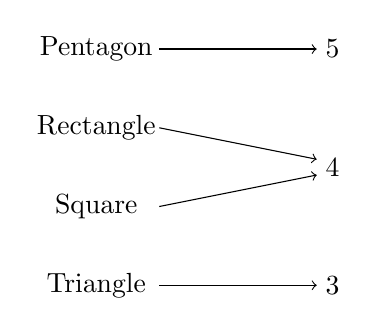
\begin{tikzpicture}
                \draw[align=right] (0, 0) node {Triangle};
                \draw[align=right] (0, 1) node {Square};
                \draw[align=right] (0, 2) node {Rectangle};
                \draw[align=right] (0, 3) node {Pentagon};
                
                \draw (3, 0.0) node {3};
                \draw (3, 1.5) node {4};
                \draw (3, 3.0) node {5};
                
                \draw [->] (0.8, 0) -- (2.8, 0.0);
                \draw [->] (0.8, 1) -- (2.8, 1.4);
                \draw [->] (0.8, 2) -- (2.8, 1.6);
                \draw [->] (0.8, 3) -- (2.8, 3.0);
            \end{tikzpicture}
            \caption{Digraph Relationship Between Polygons and the Number of Sides.}
            \label{fig:RelationshipBetweenPolygonsAndSides}
        \end{figure}
        
        Giving our relation between A and B the symbol $A \sim B$, we can also put them in a Cayley Predicate Table:
        
        \begin{table}[ht]
            \centering
            \begin{tabular}{|c|c|c|c|c|}
                \hline
                \multicolumn{2}{|c|}{\multirow{2}{*}{$A \sim B$}} & \multicolumn{3}{c|}{B} \\ \cline{3-5} 
                \multicolumn{2}{|c|}{} & 5 & 4 & 3 \\ \hline
                \multirow{4}{*}{A} & Pentagon & \cmark & \xmark & \xmark \\ \cline{2-5} 
                 & Rectangle & \xmark & \cmark & \xmark \\ \cline{2-5} 
                 & Square & \xmark & \cmark & \xmark \\ \cline{2-5} 
                 & Triangle & \xmark & \xmark & \cmark \\ \hline
            \end{tabular}
            \caption{Cayley Predicate Table of Relation Between Polynomials and Sides.}
            \label{tab:CayleyPredicateTableRelationPolynomialsSides}
        \end{table}
        
        Note from both table and digraph that $A \sim B \neq B \sim A$. In other words, it is not commutative, but we WILL discuss associativity.
        
        Discuss composition through ``matrix multiplication''. Discuss different symbolic ways to represent relations.
        
        You can notice that by looking at the Cayley Predicate Table that the checkmark (\cmark) is found exactly once per row of A. This is equivalent to saying that, on the diagraph, that there is exactly one arrow coming from each object of the shapes set.
        
        \begin{definition}
            A left-unique 
        \end{definition}
        
        A function in pure mathematics is not a function in computer science, despite that computer science is an offshoot of mathematcics (around the foundations of mathematics). The context of the word function changes in computer science to include side-effects, let's start with state and then go to sessions.
    
        Unary relations are set comprehensions
        \begin{section}{Function-Like Relations}
        \end{section}
        
        \begin{section}{Order-like Relations}
        
        \end{section}
        
        \begin{section}{Equivalence Relations}
        \end{section}
    \end{chapter}
    \begin{chapter}{Counting and Combinatorics}
        \begin{section}{adsf}
            \begin{subsection}{Relationships on the Boolean Algebra}
                \begin{align*}
                    |A \cap B| \leq |A| \quad  \textrm{and} \quad  |A \cap B| \leq |B|
                \end{align*}
                
                This is directly related to the fact that:
                \begin{align*}
                    X \subseteq Y \implies |X| \leq |Y|
                \end{align*}
                
                And this connection between these two, as important as it is, will be more thoroughly described later.
            \end{subsection}
            \begin{subsection}{Addition and the Disjoint Union}
            $$
                |A \sqcup B| = |A| + |B|
            $$
            \end{subsection}
            \begin{subsection}{Multiplication and the Cartesian Product}
            $$
                |A \times B| = |A| \times |B|
            $$
            \end{subsection}
            \begin{subsection}{Functions and Exponentials}
            $$
                |A \to B| = |B|^{|A|}
            $$
            \end{subsection}
            \begin{subsection}{Powerset as a Function}
            $$
                |\mathcal{P}(X)| = | X \to \mathbb{B} | = 2^{|X|}
            $$
            \end{subsection}
            \begin{subsection}{Permutations}
                Number of permutations = number of total orders ($|A|! = n!$)
            \end{subsection}
        \end{section}
    \end{chapter}
    \begin{chapter}{Probability Theory as a Logic}
    \end{chapter}
\end{part}
\begin{part}{Relations}
    \begin{chapter}{Binary Relations}
        \begin{section}{Heterogenous and Homogeneous Relations}
            Homogeneous means same-type, and heterogenous means different-type. In this regard, 
            
            Oftentimes, mathematically, we don't have specific words that mean possibly one and possibly the other. This is important, because a heterogenous relation can be homogenous too. The phrase non-homogenous specifically refers to a relation that must have different types.
        \end{section}
        
        \begin{section}{Heytingness}
            Make binary relation as ``included subsets'' ($R \in U\times V$) to a functional predicate for inclusion ($R : U \times V \to \mathbb{B}$) and that corresponds to ($R:U\to V \to \mathbb{B}$).
        \end{section}
        
        \begin{section}{asdf}
        \end{section}
    \end{chapter}
    
    \begin{chapter}{n-ary Relations}
    
    \end{chapter}
    
    \begin{chapter}{Relation Algebra}
    
    \end{chapter}
    
    \begin{chapter}{Other}
        A filter is a unary relation (can be useful as base-case in inductive arguments)
        
        A unary relation is a filter on a set (a subset)
        
        There are only 2 nullary relations: always holding and never holding
        
        A binary relation is a subset of the cartesian product
        
        A ternary relation requires an ordered n-tuple, since cartesian products are not associative. However, ((a, b), c) is also valid for discussion.
        
        
    \end{chapter}
\end{part}  
\begin{part}{Lambdas and Type Theory}
    \begin{chapter}{Lambdas and Combinators}
        Given our definition of functions in mathematics, we can define the truth-values of true and false as a choice. (describe by sentences and if/then).
        
        Then, we can define functions that allow us to select the first or the second part of the sentence:
        
        \begin{lstlisting}[language=Lambda]
            T x y = x
            F x y = y
        \end{lstlisting}
        
        \begin{lstlisting}[language=Lambda]
fix fib : int -> int.
  lambda n : int.
    if (n < 2) then n$^2$
    else (fib (n-1)) (fib (n-2))
\end{lstlisting}
        
        Then, the T function selects the first value, and the F function selects the second. It could just as well be called first and second, but we will define those later for a different purpose, and it will make less sense that this has anything to do with logic.
        
        Now, binding variables, in a way similar to quantifiers, we can define functions using lambdas, we will start with a function called the identify function, that gives you whatever you put in:
        
        \begin{lstlisting}[language=Lambda]
            I x = x
            I = lambda x.x
        \end{lstlisting}
        
        That is to say that the function I (again, standing for identity) is a function that takes a parameter x and returns that same argument.
        
        You will notice that instead of a symbol indicating set membership ($\in$), we separate the variable binding from the expression with the period.
        
        It may seem silly at first to have an alternative way to define a function, but the important thing is that we are not always interested in naming all of our functions. However, that's not the only benefit, the next benefit will come about as we keep talking.
        
        For now, let's define our true and false functions from before, rewriting them into lambda terms:
        
        \begin{lstlisting}[language=Lambda]
            T x y = x      T = lambda x.(lambda y.x)
            F x y = y      F = lambda x.(lambda y.y)
        \end{lstlisting}
        
        Now, again, this looks like it's creating more work, and if the goal was to express things with the least number of symbols possible, then we'd be failing. Instead. we are attempting to construct something, and the ideas will become more clear as we begin to make use of it.
        
        To apply an argument to a function looks like the following:
        
        \begin{lstlisting}[language=Lambda]
            T 3 5 = lambda x.(lambda y.x) 3 5
            T 3 5 =     (lambda y.3)   5
            T 3 5 =          3
        \end{lstlisting}
        
        The first action for application is to substitute x (the first parameter) with 3 everywhere it is used (which just so happens to be inside the parentheses). The second action is to substitute y with 5 everywhere y is found (which is not found anywhere.
        
        First things first, I want to talk about more standard order of operation (or probably more specific, ``order of interpretation'' in this case). Lambda abstractions are interpreted as right-associative, meaning that the definitions above are equivalent to:
        
        \begin{lstlisting}[language=Lambda]
            T = lambda x . lambda y . x
            F = lambda x . lambda y . y
        \end{lstlisting}
        
        \todo{discuss how this introduces us to functions that return functions}
        \todo{discuss the equivalence of this to the tuple form}
        
        Now, regarding the other operators that we'd expect from a Boolean data type, we'd expect to be able to interpret logical negation (NOT). In this case, if we logically negate the value, we swap T with F (and vice versa), which is equivalent to swapping which of the two values are selected. For instance, we'd expect the following:
        
        \begin{lstlisting}[language=Lambda]
            NOT T x y = y
            NOT F x y = x
        \end{lstlisting}
        
        So, a way that we could do this is to swap x and y:
        
        \begin{lstlisting}[language=Lambda]
            NOT p x y = p y x
        \end{lstlisting}
        
        If we used the same parameters as before, accepting T as the function that would be used:
        
        \begin{lstlisting}[language=Lambda]
            NOT T 3 5 = T 5 3
                      =   5
        \end{lstlisting}
        
        Notice that we can demonstrate the following:
        
        \begin{lstlisting}[language=Lambda]
            NOT T x y = T y x = y
                      = F x y = y
                
            NOT F x y = F y x = x
                      = T x y = x
        \end{lstlisting}
        
        So, we can say that applying NOT to T and F would give the same computed results as:
        \begin{lstlisting}[language=Lambda]
            NOT T = F
            NOT F = T
        \end{lstlisting}
        
        
    \end{chapter}
    
    \begin{chapter}{Types}
        \begin{section}{As a Pseudocomplemented Lattice}
            We discussed how function types act like the implication of a logic. Referring back to Order Theory, we also discussed Heyting Algebras and Pseudocomplements, and how the great thing about having a bounded semilattice was that we could generate a pseudocomplement from the bound.
        
            We assume that the upper bound is off limits in order to avoid Russell's Paradox on Types. However, we can attempt to find a lower-bound and use that instead. We need something that no type can be less than. Our first guess may be the unit type, but that still may not be the best type.
        
            Remember that a unit type can be passed to a function, and it can be returned from a function and then used. Imagine instead a type that cannot be constructed, and therefore it cannot return. We will call this type ``absurdity'' and it will be the bottom-element. This also means that we will often refer to it as the bottom type, and we will give it the symbol $\bot$.
        
            Therefore, we can also define our pseudocomplement (our negation) as a function that returns the bottom type: $A \to \bot$. Effectively, returning $\bot$ would be evidence that the program cannot compile (i.e. our proof fails). However, some programs are required to run forever, and so there may be situations where not returning is the correct behavior.
        
            With that out of the way, let's discuss the other property of a Heyting Algebra, that a monoid exists such that $c\wedge a \leq b \iff c \leq a \to b$. With the understanding that the $\leq$ actually means $\to$, we are looking for what meaning of $\wedge$ causes $c\wedge a \to b \iff c \to a \to b$.
        
            We have discussed previously that, when working with functions, we can call a function by $(A \times B) \to C$ or we can call it as $A \to (B \to C)$. This cartesian product is precisely the $\wedge$ we are looking for.
        
            This means that we have all the connections between the following:
            \begin{itemize}
                \item Boolean Logic (Heyting Algebras) -- $[(A\ \wedge\ B) \implies C] \iff [A \implies (B \implies C)]$
                \item Algebra -- $(c^{b})^{a} = c^{ba}$
                \item Type Theory / Functions -- $(A\times B) \to C \iff A \to (B \to C)$
                \item Category Theory -- $Hom(A \otimes B, C) = Hom(A, B \Rightarrow C)$
            \end{itemize}
        \end{section}
        \begin{section}{The Coproduct}
            We have defined the product in Type Theory now, and as we have stated, when there is a product, there is a coproduct in the opposite category. Well, we're going to skip the full categorical dual and continue discussing the relationships with the Heyting Algebra from before.
            
            Remember that, algebraically, when we have an exponential, we get the property that $(c^a)(c^b) = c^{a + b}$. It so happens that in logic, this also takes the same form that the join has: $(a \implies c) \wedge (b\implies c) \iff (a \vee b) \implies c$.
            
            So, we are looking for how to interpret $(A \to C) \times (B \to C)$, which are 2 functions, that allow us to get a type $C$ based on whether the input is $A$ or the input is $B$. In this regard, it's a choice between the inputs A and B. This has some characteristics similar to our disjoint union from set theory.
            
            We turn a proof of $A + B$ into a proof of $A$ or a proof of $B$, either of which allows us to get to $C$.
            
            In fact, we have a very perfect example of such a disjoint union available at hand:
            $$
                \mathbb{B} = T \vert F
            $$
            
            Where the ($\vert$) symbol means ``select between'', and being that T is a unit type (1), and F is also a unit type (1), then $\mathbb{B} = 1 + 1$ is sometimes denoted $2$.
        \end{section}
        \begin{section}{Peano Again}
            Now we are in a position to start defining Peano Arithmetic in Type Theory instead of plain ole Lambda Calculus. For that, we get the following:
            
            \begin{lstlisting}[language=Lambda]
                Nat = Z | S Nat
            \end{lstlisting}
            
            That is, we have the Natural Numbers defined as something that starts with zero (Z) and allows us to select a successor function (S) that takes a Natural Number as an input.
        \end{section}
    \end{chapter}
\end{part}

%----------------------------------------------------------------------------------------
%	CHAPTER 1
%----------------------------------------------------------------------------------------

\chapterimage{head2.png} % Chapter heading image

\chapter{Introduction}

\section{Motivation}\index{Motivation}
This book is a high-speed walk through the core mathematics and usages for various applications within science and engineering. It does not serve to teach proofs, or instruct on why the information contained herein works the way that it does, but instead serves to move straight to the heart of application.

The point of this book is to treat everything as computation. We will study arithmetic computations, algebraic computations, infinitesimal calculus, a calculus of sets, probability theory, statistics, etc. Until we have thoroughly gone through many of the most industry useful methodology.

The problem with this book is that it will make mathematics look as if it is about manipulating symbols in kind of ``mathematical language''. The duty and work of mathematicians was to create a system where it was possible that such symbolic manipulation is possible.

Worse yet, it allows one to forget that mathematicians are actively busy coming up with new things all the time. However, it's not the goal of this book to convince the reader of that. There are additional books in the series that are tuned to explaining just how we got where we are, and where we are going.

\chapter{Algebra/Working with Expressions}
The biggest difference between arithmetic and algebra is that arithmetic was interested in working with values and performing calculations on them. Algebraic manipulation is very effective, because there are plenty of things that can be put into an algebraic context, and then manipulated the way that we manipulate algebraic expressions.
\section{Expressions}
\begin{definition}{Expression}
A mathematical expression is a well-formed collection of symbols arranged according to rules called \textbf{syntax}.
\end{definition}

The symbols may represent operations, constants, variables, functions, brackets, etc. The brackets typically explicitly give the order of operations for the expression. When the symbols are omitted, a standard order of operations are accepted.

\section{Order of operations}
In order to understand the order of operations, it's important to start with the natural numbers.

\begin{remark}
    Natural numbers are the \emph{only} type of object where multiplication is repeated addition, and where exponentiation is repeated multiplication.
\end{remark}

This is only a means of remembering the order of operation, and is not directly a reason for how the order of operations became a commonly used standard. However, the definition, going into addition, multiplication, and exponentiation separate these operations into the following levels:

\begin{tabular}{|l|l|l|l|} \hline
Level & Action & Inverse Action \\ \hline
1 & Addition & Subtraction \\ \hline
2 & Multiplication & Division \\ \hline
3 & Exponentiation & \\ \hline
4 & Function Application & \\ \hline
5 & Brackets & \\ \hline
\end{tabular}

Therefore, if one gets the following expression, where $x=5$:

\begin{equation}
2(x-1)^3+\log(5+x)=0
\end{equation}

One works left-to-right, but starts with the highest level expressions first:

\begin{equation}
\begin{aligned}
2(5-1)^3+\log(5+5)& = 0 & \textsf{Expression with Substitution} \\
2(4)^3+\log(10)&=0 &\textsf{Brackets} \\
2(4)^3+1&=0&\textsf{Function Application} \\
2(64)+1&=0&\textsf{Exponentiation} \\
128+1&=0&\textsf{Multiplication} \\
129&=0&\textsf{Addition}
\end{aligned}
\end{equation}

\section{How to look at algebra}
For equations, we have the rule that, for any expression $x=y$ and any function ``f'':


Demonstrate to reader how this next equation is a consequence of equivalence classes...
\begin{equation}
x=y \Leftrightarrow f(x)=f(y)
\end{equation}

\part{Topics}
Foundational parts
\begin{itemize}
    \item Categories (logic and order)
    \item Model Theory (sets, types, etc.)
    \item Algebraic Theories (axiomatic definitions and symbolic manipulations through orders)
    \item Topology (including calculus)
\end{itemize}


\begin{itemize}
    \item The different meanings of equality: isomorphism vs identity
    \item Multiplication and addition as more fundamental than division or subtraction, with the exception of how subtraction is actually a distance function
    \url{https://www.quora.com/Do-we-need-division-and-subtraction-as-separate-operations-when-division-can-be-written-as-a-factor-with-the-exponent-of-1-and-subtraction-of-a-term-as-an-addition-of-the-negative-term-a-div-b-a-cdot-frac-1-b-a-b-a/answer/Nicholas-Cooper-8}
    
    \item That imaginary numbers are as imaginary as real numbers:
    \url{https://www.quora.com/Are-all-numbers-really-imaginary-numbers-How-are-numbers-real/answer/Nicholas-Cooper-8}
    \url{https://www.quora.com/What-real-world-phenomena-can-be-quantified-with-imaginary-numbers/answer/Nicholas-Cooper-8}
    
    \item The truth about measurements
    \url{https://www.quora.com/A-scalar-quantity-can-t-be-negative-because-it-only-has-magnitude-but-no-direction-but-why-can-temperature-can-be-negative/answer/Nicholas-Cooper-8}
    
    
\end{itemize}


%----------------------------------------------------------------------------------------
%	CHAPTER 3
%----------------------------------------------------------------------------------------
\printglossaries
\end{document}

\end{part}

\part{Mathematical Introduction to Philosophy}
%----------------------------------------------------------------------------------------
%	TABLE OF CONTENTS
%----------------------------------------------------------------------------------------

\chapterimage{head1.png} % Table of contents heading imag

%\cleardoublepage % Forces the first chapter to start on an odd page so it's on the right

\pagestyle{fancy} % Print headers again

Every symbol used in mathematics is like a pronoun is in natural language. When I say ``Cameron gave away his guitar'', you know that the word ``his'' is in reference to Cameron through context. Oftentimes, we are telling you want we want each variable, operator, and symbol to mean, but oftentimes, you will have to recognize the symbols from previous work.


\begin{chapter}{Introduction to Philosophy}
    No book that mentions philosophy is complete without describing those things that are intended, or valued as goals from the book, or in corporate speak a ``vision'' for the book. This is why this book does not have a formal introduction, but finds an introduction in this section, serving to introduce the importance of formalizing goals when doing work:
        
    \begin{section}{The Intended Value of this Book}
        This is a mathematics book, and the goal of this book is to teach mathematics. However, there are many books which aim to teach mathematics, but the author feels as if there is much missing in the way of:
            
        \begin{itemize}
            \setlength{\itemsep}{6pt}
            \setlength{\parskip}{12pt}
                
            \item \textbf{Intuitions} for the concepts being taught are not commonly taught because our intuitions can often lead us astray. Oftentimes, when we teach analogies, people assume the analogies are more real than analogous, and get angry and upset when the analogies fall apart. Therefore, a long discussion must be had to explain that an analogy doesn't necessarily mean something is equivalent.
     
            \item \textbf{Examples and motivations} of the concepts being used by people. This does not mean that every example needs to be something that is used by everyone, on a daily basis. Mathematics is often argued to be independent from the physical world, and despite the truth in that, the mathematicians who discover these things are not independent of the physical world, and so the physical world still informs the mathematician, and the learner.
               
            \item Because we will focus on examples and motivation from things in the physical world, we will also add \textbf{computer programming} to our learning curriculum, building up to it, nearly from the beginning. This will be a help and a hindrance, because computer literacy and knowledge of how to set up programming environments is not a focus of the lesson plans here. In fact, we should learn what the mathematical concept of a computer is, which is not necessarily the physical thing that this book was written on, but relates to it to a very strong degree.
                
            \item Along the line of the focus on examples, we will collect \textbf{interpretations} of mathematics as it is discussed, and disseminate those interpretations as best possible.
                
            \item Furthermore, the most important thing we will do is to connect various areas of mathematics, so that intuitions from one area will carry over to the other areas, and so will the proofs. Due to this, we may prove some theorems in more than one way in this book, so that the connections can be understood, and to help demonstrate what a theorem really is.
        \end{itemize}
            
        However, the additional focus on the things listed above does not imply that this book can avoid any of the items below, and must be discussed in balance, and with sufficient detail with the following: 
            
        \begin{itemize}
            \setlength{\itemsep}{6pt}
            \setlength{\parskip}{12pt}
                
            \item Formal definitions and descriptions of the concepts, including axiomatic definitions for mathematical structures
                
            \item Various constructions of mathematical structures when possible
                
            \item Formal reasoning for the properties of mathematical structures
        \end{itemize}
            
        You'll notice that these 3 all focus on mathematical structures, which may seem like a foreign concept right now. However, we will provide some heightened understanding of what a mathematical structure is by the end of this book.
            
        The intended reader of this book is adults, and in that respect, it is andragogy (the study of teaching adults), not pedagogy (the study of teaching children). It assumes certain concepts are already understood (like an intuitive feel for the number 250, and of place-value in general); however, it is the author's opinion that the order of subject matter given in this book is approximately the best order to teach children as well, given the mathematical subject matter available as of the year 2020.
    \end{section}
        
    \begin{section}{Motivation to Learn and a Warning to Learn it Well}
        \begin{subsection}{Knowledge is One Source of Strength}
            \begin{quote}{Edward Teller}
                The science of today is the technology of tomorrow.
            \end{quote}
            
            \begin{quote}{Chinese Proverb}
                If your mind is strong, all difficult things will become easy. If your mind is weak, all easy things will become difficult.
            \end{quote}
                
            Since we are still talking about philosophy, another good argument to learn philosophy, and to learn it well, is to build a strong mind through careful analysis of: your values, your own value, what makes you strong, and how you come to understand the world around you.
                
            However, the journey through these analyses are usually very personal. The last one, ``how you come to understand the world around you'' is the only one that this book intends to address in great detail, but being a mathematical book, and not a science book, it's actually less about understanding the physical world, and more about understanding what intuitions are actually happening in your own mind.
                
            We add mathematics to this study, because we realize what it brings to our society, as far as strength goes, by giving us these glimpses into the role that our intuitions have regarding how we interpret the world around us, and how those intuitions sometimes fail, and how often they actually succeed.
                
            The role of mathematics for our society is usually at one end of the chain of information that occurs between the various STEM-based subjects:
                
            \begin{figure}[ht]
                \centering
                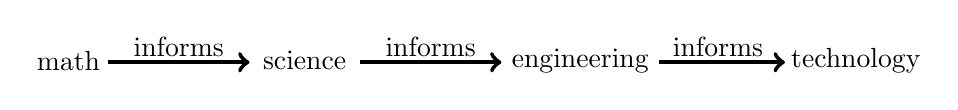
\begin{tikzpicture}
                    \node [align=center] at (0.0, 0.02){math};
                    \draw [ultra thick, ->] (0.5, 0) -- (2.3, 0);
                    \node [align=center] at (1.4, 0.2){informs};
                    \node [align=center] at (3.0, 0.02){science};
                    \draw [ultra thick, ->] (3.7, 0) -- (5.5, 0);
                    \node [align=center] at (4.6, 0.2){informs};
                    \node [align=center] at (6.5, 0.02){engineering};
                    \draw [ultra thick, ->] (7.5, 0) -- (9.1, 0);
                    \node [align=center] at (8.25, 0.2){informs};
                    \node [align=center] at (10, 0.02){technology};
                \end{tikzpicture}
            \end{figure}
                
            However, you'll also find that philosophy informs all of these, and is informed by all of these. The creative arts, like philosophy, is informed by all 4 of these, but tends towards informing only engineering and technology.
                
            This does not mean that mathematics and science is not creative, but it's often misunderstood that because mathematics is so rational, that it's not creative. It takes a lot of creative thinking and intuition, along with rational thought, in order to come up with mathematical proofs, and it is for this reason, and the connections to other fields, that creative arts is a necessary endeavour for anyone learning STEM.
                
            In fact, this is precisely the argument for STEAM.
                
            It must be stated more clearly, because the previous statement may not be clear enough: creative thinking, intuition, and rational thinking are \textbf{all} required for work in each of these fields of study, in concert with each other. Rational thinking does not promote mathematics and science alone. Intuitional thinking will almost certainly lead to falsehoods in these fields, if not matched with rational thinking.
                
            In this sense, creative thinking can be seen to be exploration, finding solution-after-solution, intuitive thinking can be seen to point the creative thinking along, but the rational thinking is the filter that finds the solutions that actually work.
                
            So, you will benefit all of these parts of your mind, including the part of you that is disciplined and builds grit. This will happen by mere practice and use, much like a muscle being used over-and-over getting bigger, and capable of handling more.
                
            Mathematics and the sciences change how you look at the world around you, but it doesn't make you a better person.
        \end{subsection}
        
        \begin{subsection}{The Danger in Strength}
            Philosophy has a long history of beneficial usage and of dangerous misuse. Philosophy may be the most important, but the most dangerous subject matter that a mind can consume. Philosophy has been used to free people as well as enslave people. The philosophical concept of moral or ethical \emph{justification} has been used both to protect and to kill.
            
            In effect, every argument about whether or not human beings are ready for a specific technology is actually a question of whether or not human beings are philosophically mature enough, and is captured in the following quotes:
            
            \begin{quote}{Jason Silva}
                Technology is, of course, a double-edged sword. Fire can cook our food but also burn us.
            \end{quote}
            
            \begin{quote}{Christian Lous Lange}
                Technology is a useful servant, but a dangerous master.
            \end{quote}
            
            \begin{quote}{B. F. Skinner}
                The real problem is not whether machines think, but whether people do.
            \end{quote}
            
            Replace ``technology'' with ``philosophy'' in the first two quotes, and you may begin to understand what it is that I'm claiming. Other quotes are a bit more direct:
            
            \begin{quote}{Martin Luther King, Jr}
                Nothing in all the world is more dangerous than sincere ignorance and conscientious stupidity.
            \end{quote}
            
            \begin{quote}{George Bernard Shaw}
                Beware false knowledge; it is more dangerous than ignorance
            \end{quote}
            
            \begin{quote}{Confucius}
                Real knowledge is to know the extent of one’s ignorance
            \end{quote}
            
            Oftentimes, it is exactly those strengths that serve as one's weaknesses, but that is not to say that having a strength necessarily creates weakness in that area. It benefits us to understand how strengths become weaknesses. 
    
            Philosophy, like technology, is good or bad, depending on how it's used, and depending on how well it's understood, and based on what principles one chooses to work from.
                
            In fact, the call-to-action I give each of you, before you start this endeavour is:
            \begin{itemize}
                \item Use your observations and experiences to help you understand your world
                    
                \item Uproot misperceptions and misunderstandings that come from a partial understanding of the first
                    
                \item Apply your understanding of the world to better your world and the world of others, as you see fit
            \end{itemize}
        \end{subsection}
        
        \begin{samepage}
            \begin{subsection}{Perceptions and Misperceptions of Philosophy, Mathematics, and Science}
                There are multiple misperceptions of about various fields of study, such as:
                \begin{itemize}
                    \item Mathematics
                    \begin{itemize}
                        \item It's not a creative field
                        \item It's the study of numbers
                        \item It's already finished (there's no new math to be had)
                        \item There are no jobs for mathematicians
                    \end{itemize}
                    
                    \item Science
                    \begin{itemize}
                        \item It's done by elite people who have no connection to reality
                        \item It's a collection of statements that are considered ``the truth''
                        \item It doesn't help ``real people''
                    \end{itemize}
                    
                    \item Software Development
                    \begin{itemize}
                        \item It's all copy-and-paste
                        \item Computers will be programming themselves soon
                        \item It's an easy desk-job with little pressure
                    \end{itemize}
                        
                    \item Economics
                    \begin{itemize}
                        \item It's the study of money
                        \item It's all psychology (which contradicts the first claim)
                    \end{itemize}
                \end{itemize}
            \end{subsection}
        \end{samepage}
            
        All of these claims are caricatures of the fields of study, or of the people who do work in those fields, and are not just oversimplifications, but are outright wrong if one were to actually follow these people around.
            
        Much the same misrepresentation occurs in all fields of study and all fields of work. These misrepresentations continue throughout the centuries as populism attempts to change the view of these subjects.
            
        The history of this populism is understood, because in history, fields such as these could only be achieved by the educated and the rich, and those people would not understand those who worked with their hands. Therefore, a schism occurred between those who used their minds, and those who used their hands, based on a classism that is not yet resolved.
            
        A shift has been occurring over the last few centuries though, especially as education has become more universal, allowing people to spend part of their lives in service, part of their lives in manual labor, part of their lives studying, and part of their lives working with their minds, and it's not certain that a person in any particular job has any particular experience.
            
        In this regard, philosophy has always been misrepresented, and you may hear things like:
        \begin{enumerate}
            \item Philosophy, like mathematics, has been completed, or it has produced all of the results and discoveries that it can
                
            \item Philosophy is useless, ungrounded, and a waste of a person's education
                
            \item Philosophy is nebulous, vague, and done by people who are out-of-touch with the real-world
                
            \item Philosophy opposes, is not supported of, or is somehow separate from science
        \end{enumerate}
            
        Nothing could be further from the truth on all of these grounds. Mathematics, and philosophy, are coming up with new discoveries all the time, and including applications to previous discoveries. Philosophy, especially the interest of how we come to know things, forms the basis for both mathematics and the sciences.
    \end{section}
    
    \begin{section}{What is Philosophy, and Why Should We Care?}
        Philosophy is typically introduced by discussing what it means, and where it comes from. We focus so much on the Greek philosophy, but philosophy, mathematics, and science has been growing in all cultures for millennia, and can be found as early trial versions of these subjects in ancient books all over the world.
            
        The word ``philosophy'' is a word from ancient Greek φιλοσοφία (\emph{philosophía}), which has 2 roots:
        \begin{itemize}
            \item φίλος (phílos meaning “loving”)
            \item σοφία (sophía meaning “wisdom”)
        \end{itemize}
            
        However, that only scratches the surface, and tends to lead to the conclusion that “philosophy is in every query”. Although this is technically true, it does little to give anyone any clue to what philosophers actually do, and why it’s important.
            
        In some ways, philosophy is the process of exploring one’s thoughts, asking ourselves, “why do I think this way?”
            
        Specifically, philosophers have certain question that all philosophy branches out from:
            
        \begin{figure}[ht]
            \centering
            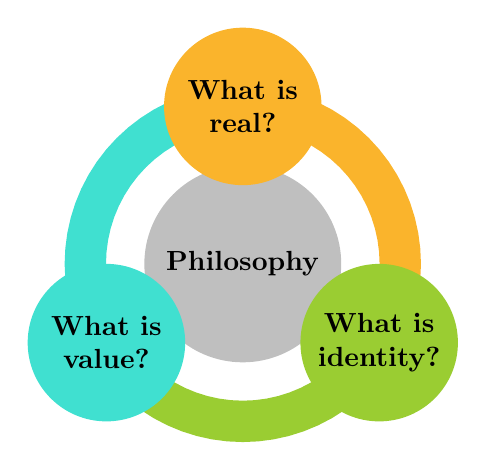
\begin{tikzpicture}
                \fill [lightgray]   (0,0) circle (12.5mm);
                \node [align=center] at (0, 0) {\textbf{Philosophy}};
                \draw [Dandelion,line width=5.25mm,domain=-30:90] plot ({2*cos(\x)},     {2*sin(\x)});
                \draw [YellowGreen,line width=5.25mm,domain=210:330] plot ({2*cos(\x)},     {2*sin(\x)});
                \draw [Turquoise,line width=5.25mm,domain=90:210] plot ({2*cos(\x)},     {2*sin(\x)});
                \fill [Dandelion] (0,2) circle (10mm);
                \fill [YellowGreen] ( 1.732,-1) circle (10mm);
                \fill [Turquoise]   (-1.732,-1) circle (10mm);
                \node [align=center] at ( 0.000, 2) {\textbf{What is}\\\textbf{real?}};
                \node [align=center] at ( 1.732,-1) {\textbf{What is}\\\textbf{identity?}};
                \node [align=center] at (-1.732,-1) {\textbf{What is}\\\textbf{value?}};
            \end{tikzpicture}
            \caption{The 3 Proposed Root Questions of Philosophy.}
            \label{fig:ThreePhilosophicalQuestions}
        \end{figure}
            
        Here though, these 3 questions feed off of each other. For instance, 
        \begin{itemize}
            \item Is it possible to seek truth without asking what methods of truth-seeking that we value?
                
            \item If something exists (if it’s “real” or “true”), can we identify it?
                
            \item If we change something (identity) does it change value?
        \end{itemize}
            
        In fact, these three questions spawn multiple branches of study, some of which are considered philosophical in modern times still, others may appear, on the surface, as if they are something separate from philosophy.
            
        \begin{subsection}{What is Real?}
            Epistemology relates to the question, “How do we know what we know?”. The study     of epistemology has given us logic (forming the foundations of mathematics),     the Scientific Method (forming the foundations of science), and gives us     mechanisms for us to understand beliefs by asking:
                
            \begin{itemize}
                \item What does it mean to know something?
                \item Can anything be known for certain? 
                \item How much confidence can we have in something?
                \item What is the process that we come to know things?
                \item What does it mean to know things?
                \item What is a belief?
                \item Can we justify our beliefs? (\textbf{critical reasoning})
                \item What is the relationship between beliefs and knowledge?     (\textbf{doxastic logic})
            \end{itemize}
        \end{subsection}
            
        \begin{subsection}{What is Identity?}
            In philosophy, we talk about \textbf{discernibility}, which lets us ask, “if two things share all the same properties, are they the same thing?”. We use this in mathematics to present two things being equal. In science, we identify phenomena that interest us. In our lives, we discuss personal identity, social identity, and even discuss the human identity. In many ways, the philosophical focus on definitions and on meanings are directly related to identifying concepts, and coming to agreement on concepts, in order to help discuss.
                
            It leads us to questions like:
                
            \begin{itemize}
                \item What does it mean for two things to be the same, and does that change over time or based on the context?
                \item If I replace every component with an identity component, is it the same thing (Interchangeability and compatibility)?
                \item Are we the same person from one moment to the next?
                \item Is any object the same from one moment to the next?
                \item How do we relate to and do we identify with our city, our culture, and/or our nation?
                \item What does it mean when things are “almost alike” or similar? And do similar things share similar properties?
            \end{itemize}
        \end{subsection}
        \begin{subsection}{What is Value?}
            The notion of \textbf{value} or \textbf{worth} is also of central concern, as it allows us to compare two things. This is also of central concern in mathematics as it allows us to make statements about relationships between things. It is of concern in modern politics, when discussing the value of citizens and whether or not they feel valued. We discuss \textbf{aesthetics} as the study of those things that attract our senses. We discuss \textbf{ethics} through the value of actions. It leads us to questions like:
                
            \begin{itemize}
                \item What does it mean to compare two things?
                \item Why do things cost what they do?
                \item What do individuals value, and why?
                \item What do societies value, and why?
                \item Is something practical worth more than something else? What makes it practical?
                \item What is fairness and justice?
            \end{itemize}
        \end{subsection}
        \begin{subsection}{What is the Relationship Between Value and Identity?}
            When questions about both value and identity come together, we usually start to ask about purpose, and
            \begin{itemize}
                \item Is there a purpose to the existence of the universe? What is the purpose?
                \item Is there a purpose to my existence? What is the purpose? Do I create my own purpose?
                \item Am I a valued part of my community? Why or why not?
                \item What is fair when it comes to treatment of different people?
                \item How does interchangeability relate to comparison? If I interchange components for something newer, is it better?
            \end{itemize}
        \end{subsection}
        \begin{subsection}{What is the Relationship Between Value and Truth?}
            This is the intersection of the two questions that lead us to asking questions like:
            \begin{itemize}
                \item How do we value the various means of obtaining knowledge?
                \item How do people value methods of communicating knowledge and beliefs?
                \item Whose testimonies do we believe and why?
                \item Can there be an absolute, top-level truth, by which all other truths are measured?
                \item Can there be a best moral code, by which all other moral codes are measured?
            \end{itemize}
        \end{subsection}
        \begin{subsection}{What is the Relationship Between Identity and Truth?}
            Regarding identity and truth, we may get some interesting questions about ourselves and:
            \begin{itemize}
                \item What are we? (i.e. what makes us human, or what makes us different?)
                \item Where do we come from?
                \item Why does anything exist at all?
                \item How do we relate to our perceptions, and vice versa?
                \item What does it mean to “exist”?
                \item What does it mean to be “real”?
                \item What is reality?
                \item What is the mind?
            \end{itemize}
        \end{subsection}
        \begin{subsection}{What is the Relationship Between All 3?}
            Finally, we can consider all 3 together:
            \begin{itemize}
                \item Is there something bigger than us?
                \item What is out there, beyond what we can perceive?
                \item How did this universe come to exist? (\textbf{cosmology})
                \item What is the greatest possible mind? Must a creator exist? (\textbf{theology})
            \end{itemize}
        \end{subsection}
            
        \begin{subsection}{Categorizing the Questions into Branches}
            Many of these questions have been placed into various categories:
            \begin{itemize}
                \item That reason can be a source of knowledge (\textbf{rationalism}) allowed us to create logic, and logic continues to refine the foundations of mathematics (classically called, “the formal sciences”)
                    
                \item Critical thinking, using our senses as a source of knowledge (\textbf{empiricism}), building confidence through experimentation (\textbf{verificationism}), and filtering in only those things that we can derive from these sources (\textbf{positivism}) refines the scientific method, which gives us science (classically called, “the physical sciences”)
                
                \item Questions about value form the basis for \textbf{Value Theory}, and include subbranches like: ethics, aesthetics, and axiology (moving into application through economics and politics)
                    
                \item Questions about existence and reality form the basis of \textbf{Metaphysics}, and include subbranches like: theology, religion, and ontology 
                    
                \item Questions about how we do philosophy form the basis of \textbf{Metaphilosophy}
            \end{itemize}
        \end{subsection}
    \end{section}
    
    \begin{section}{Philosophical Discussions}
        So, you thought that this book was going to be about mathematics. Why, then, are we learning philosophy? Well, it turns out that philosophy is the parent of almost every subject studied in any formal education. 
            
        Given that we have asked about reality, science is a formal discipline of the philosophical position called empiricism, allowing us to enter into discussion about those areas of discussion that can be observed and measured with repeatable results. However, as positions go, science is limited to such discussions.
            
        Foremost, we are interested in mathematics in this book, but we will only really get there by discussing the roots of mathematics. Also, in order to understand it, we will do best when we can also link our study to various other areas as well. The most interesting part is how these things link.
            
        \begin{figure}[ht]
            \centering
            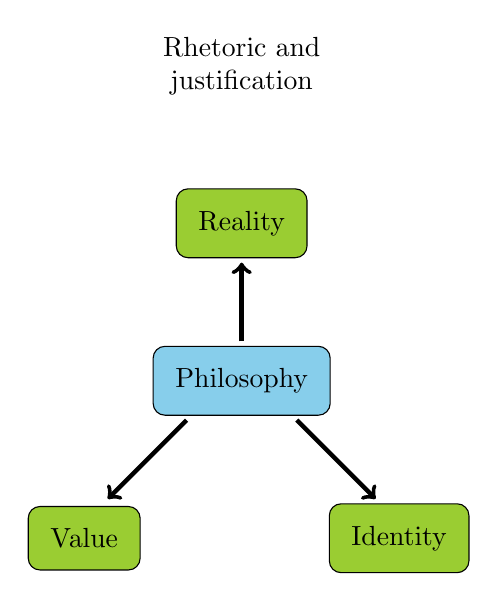
\begin{tikzpicture}
                \node [align=center,draw=black,fill=SkyBlue,thin,inner sep=8pt,rounded corners=.15cm] at (0.0, 0.0) {Philosophy};
                
                \node [align=center,draw=black,fill=YellowGreen,thin,inner sep=8pt,rounded corners=.15cm] at (0.0, 2.0) {Reality};
                
                \node [align=center] at (0.0, 4.0) {Rhetoric and\\justification};
                
                \node [align=center,draw=black,fill=YellowGreen,thin,inner sep=8pt,rounded corners=.15cm] at (-2, -2.0) {Value};
                
                \node [align=center,draw=black,fill=YellowGreen,thin,inner sep=8pt,rounded corners=.15cm] at ( 2, -2.0) {Identity};
                
                \draw [ultra thick, ->] ( 0.0, 0.5) -- (0.0, 1.5);
                \draw [ultra thick, ->] (-0.7,-0.5) -- (-1.7, -1.5);
                \draw [ultra thick, ->] ( 0.7,-0.5) -- ( 1.7, -1.5);
                %\node [align=center] at (0.0, 0.02){math};
                %\draw [ultra thick, ->] (0.5, 0) -- (2.3, 0);
                %\node [align=center] at (1.4, 0.2){informs};
                %\node [align=center] at (3.0, 0.02){science};
                %\draw [ultra thick, ->] (3.7, 0) -- (5.5, 0);
                %\node [align=center] at (4.6, 0.2){informs};
                %\node [align=center] at (6.5, 0.02){engineering};
                %\draw [ultra thick, ->] (7.5, 0) -- (9.1, 0);
                %%\node [align=center] at (8.25, 0.2){informs};
                %\node [align=center] at (10, 0.02){technology};
            \end{tikzpicture}
        \end{figure}
            
        \begin{figure}[H]
            \centering
            \includegraphics[scale=0.65]{PhilosophicalIntroduction/ConnectionsToPhilosophy.png}
            \caption{Connections of Various Fields to Philosophy.}
            \label{fig:ConnectionsToPhilosophy}
        \end{figure}
            
        \begin{subsection}{Rhetoric and Justifying Beliefs}
            It's important to understand that much of our mental sophistication revolves around explaining ourselves to others, whether that be in regards to giving them a mental image of what we have seen, explaining how something works, to justifying our reasons for doing something.
                
            Jonathan Haidt gave us the analogy of our minds being of a human rider on top of an elephant, whereas the rider is the rational mind, and the intuition is the elephant. We are so good at justifying our actions to others, that we often justify things we have done to ourselves, even when we know better (e.g. ``I can eat that whole chocolate cake, because I've done so well on my diet this week.'').
                
            Our written Greek philosophy seems to start with regards to \textbf{rhetoric}, as the ``art of discussion'', developing the communication skills to discuss philosophical positions.
                
            Rhetoric was often divided into:
            \begin{itemize}
                \item \textbf{Emotional} appeals, intended to speak directly to the mind's elephant. These appeals are often highly effective, if sometimes manipulative in their usage.
                    
                \item \textbf{Authoritative} appeals, intended to invoke the authority of the speaker, through their experience or due to their character-history of truthfulness.
                    
                \item \textbf{Rational} appeals, intended to speak directly to the rider of the elephant, who is capable of mapping out a direction for the elephant to travel, if the rider can ever get the elephant to listen.
            \end{itemize}
                
            We may be used to hearing the word rhetoric in political discussions (such as ``inflammatory rhetoric''), but oftentimes the person using the word doesn't mean it with the nuance of the philosophical meaning. Instead, philosophers would deem what politicians are doing \textbf{polemic}, which is emotional arguments intended to reduce confidence in and incite fear of an opponent.
                
            It should be obvious that mathematics and the sciences are filled with logical appeals, and as such, this book will be filled with them as well. However, it's also recognized that the intuition must be brought on board as well. 
                
            Finally, the authoritative appeals should be mostly unused in any discussion of mathematics. There is no for a teacher to use appeals to authority, saying things like ``it just works this way''. The only authoritative appeals will be the usage of already defined and commonly used standards for writing that may be brought up. However, even those should be backed with arguments for rational reasons why.
                
            \begin{subsubsection}{Some Definitions}
                
                \begin{definition}
                    An \textbf{interlocutor} is a person that is taking part in a dialog.
                \end{definition}
                    
                \begin{definition}
                    A \textbf{proposition} is a statement is possibly true or false.
                \end{definition}
                    
                \begin{definition}
                    A \textbf{premise} is a proposition for consideration, sometimes asserted as true by the interlocutor, and sometimes as a condition for the context of the argument.
                \end{definition}
                    
                \begin{definition}
                    A \textbf{conclusion} is a proposition that is the end result that the interlocutor reaches starting from the premises.
                \end{definition}
                    
                \begin{definition}
                    An \textbf{argument} is a series of propositions, structured such that the premises lead to a conclusion. Furthermore, a more general meaning of this word may be a process of reasoning.
                \end{definition}
                    
                \begin{definition}
                    A premise taken as a condition, usually in regards to an investigation is called a \textbf{hypothesis}.
                \end{definition}
                    
                \begin{definition}
                    A \textbf{philosophical position} is a collection of premises that an interlocutor is arguing from.
                        
                    It is often called a \textbf{philosophical theory}, which can cause confusion with the significantly different meanings taken by scientific theory and mathematical theory. 
                        
                    The everyday usage of the word ``theory'' is probably best identified as ``hypothesis''.
                        
                    Due to this confusion, the word position will be preferred in this book.
                \end{definition}
                    
                \begin{figure}[ht]
                    \centering
                    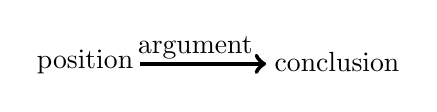
\begin{tikzpicture}
                        \node [align=right] at (0.0, 0.02){position};
                        \draw [ultra thick, ->] (0.7, 0) -- (2.3, 0);
                        \node [align=center] at (1.4, 0.2){argument};
                        \node [align=left] at (3.2, 0.02){conclusion};
                    \end{tikzpicture}
                    \caption{Relation between position (premises), argument, and conclusion}
                \end{figure}
                    
                \begin{definition}
                    For the sake of comparison, a \textbf{life stance} is a philosophical position that one takes, according to their worldview, which informs their beliefs, their thoughts, and their behavior.
                        
                    This is stated separately, since a life stance differs from a philosophical position.
                \end{definition}
                    
                \begin{definition}
                    A \textbf{Devil's Advocate} is a person that argues from a position that differs from their life stance, in order to better understand their own position, and the position of others.
                \end{definition}
                    
                \begin{definition}
                    \textbf{Skepticism} is the act of reserving belief for future evidence.
                \end{definition}
                
                \begin{definition}
                    \textbf{Belief revision} is the act of modifying one or more premises that make up a position, due to new evidence.
                \end{definition}
            \end{subsubsection}
            
            \begin{subsubsection}{What Forms a Worldview}
                At this point, I'm going to present what follows as a position, setting the rest of the book up for discussions on logical reasoning.
                    
                \begin{remark}
                    This position I am starting from, regarding worldviews, is not scientific, is not based on psychological evidence, and is likely just an approximation of how worldviews actually work.
                \end{remark}
                    
                \begin{figure}[ht]
                    \centering
                    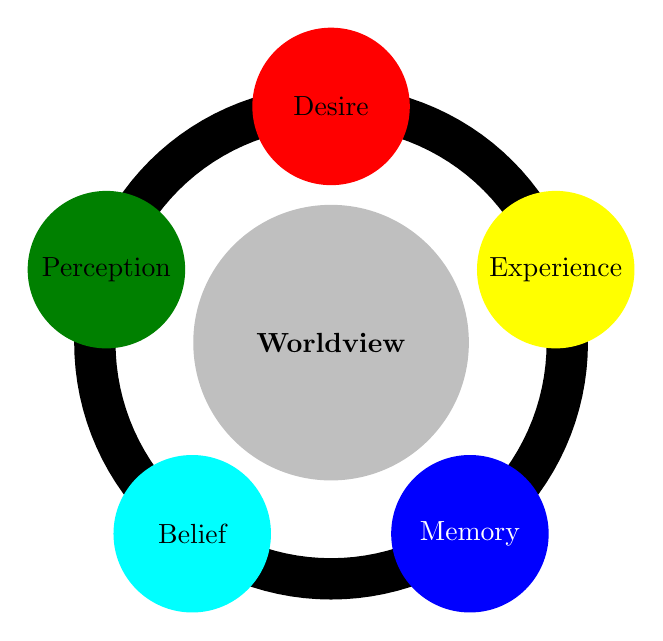
\begin{tikzpicture}
                        \fill [lightgray] (0,0) circle (1.75cm);
                        \node [align=center] at (0, 0) {\textbf{Worldview}};
                            
                        \draw [Black,line width=5.25mm,domain=90:162] plot ({3*cos(\x)}, {3*sin(\x)});
                        \draw [Black,line width=5.25mm,domain=162:234] plot ({3*cos(\x)}, {3*sin(\x)});
                        \draw [Black,line width=5.25mm,domain=234:306] plot ({3*cos(\x)}, {3*sin(\x)});
                        \draw [Black,line width=5.25mm,domain=306:378] plot ({3*cos(\x)}, {3*sin(\x)});
                        \draw [Black,line width=5.25mm,domain=378:450] plot ({3*cos(\x)}, {3*sin(\x)});
                            
                        \fill [Red]   ( 0.000000, 3.000000) circle (10mm);
                        \fill [Green] (-2.853170, 0.927051) circle (10mm);
                        \fill [Cyan]  (-1.763356,-2.427051) circle (10mm);
                        \fill [Blue]  ( 1.763356,-2.427051) circle (10mm);
                        \fill [Yellow]( 2.853170, 0.927051) circle (10mm);
                            
                        \node [align=center,text=black] at 
                        ( 0.000000, 3.000000) {Desire};
                        \node [align=center,text=black] at 
                        (-2.853170, 0.927051) {Perception};
                        \node [align=center,text=black] at 
                        (-1.763356,-2.427051) {Belief};
                        \node [align=center,text=white] at 
                        ( 1.763356,-2.427051) {Memory};
                        \node [align=center,text=black] at 
                        ( 2.853170, 0.927051) {Experience};
                    \end{tikzpicture}
                    \caption{Relation between position (premises), argument, and conclusion}
                \end{figure}
                    
                The first question someone may have looking at the components of a person's worldview that I listed is that experience, memory, and belief are all the same thing. However, my argument is that we experience all the time, but our beliefs color how we interpret the memories associated with those experiences.
                    
                In this sense, we reexperience things through our memory, but it doesn't mean that it feels the same each time.
                    
                It may seem strange that I put desire in with the rest of these, because it appears that the rest of these relate to knowledge, but that desire is completely unrelated. However, we already know that desires change how we perceive things, making us more or less perceptive of our failures or successes, or how other people act.
                    
                The point of all of this is to say that our memories are fallible, because they change. Our perceptions are fallible as well, and so, we cannot always trust our worldview.
            \end{subsubsection}
                
            \begin{subsubsection}{What Sources of Information do you Value?}
                In the discussion of rhetoric, we talked about 3 different types of arguments: emotional, authoritative, and rational.
                    
                However, these are only the methods of transference of information from one person to another, and misses an important source of information: experience.
                    
                We tend to regard experience as the most valued source of information, but as we discussed in regards to the worldview, our perceptions of experiences are often incomplete, and sometimes even wrong.
                    
                Most people, naturally value emotional, authoritative, experiential, intuitive, and rational information sources to some level or another, because we naturally recognize that there are failings with putting all of our trust in any one of them: emotions can sometimes be erratic, people sometimes lie, our perceptions often deceive us, our intuitions are often wrong, and we often don't have enough information to come to a rational conclusion.
                    
                However, there are things that we can do to refine when we use each, and what we can be said about each source of information.
                    
                Firstly, it's important to note that rational arguments begin as intuitive arguments. Humans have an intuitive ability to recognize cause-and-effect, allowing us to determine how things work, and often change how things work to our favor. This recognition of the pattern of cause-and-effect is what leads us to logic, and rational thinking is the disciplined use of this logic. 
                    
                In fact, the discipline is what separates intuition from rational thinking. We follow through with our intuitions to see if they fail.
                    
                Second, the relationship between emotions and intuition are also important. Purely rational thinking is devoid of creativity, can get stuck in analysis, and therefore absent problem solving ability. However, purely intuitive thinking cannot weed out those ideas that won't work, and will naturally try things that are not logically sound, usually wasting their own and other people's time.
                    
                First, let's get more detailed how these each operate as a source of information:
                \begin{itemize}
                        
                    \item Authoritative sources
                    \begin{itemize}
                        \item \textbf{Witnesses} can provide accounts of events
                        \item Parents and teachers often provide us tons of information
                    \end{itemize}
                    \item Experiential sources
                    \begin{itemize}
                        \item Your \textbf{senses} give you access to the world around you and are your connection to it
                        \item When your senses act together they create an \textbf{empirical} view of the world
                        \item This effectively places you as an authority over your own worldview
                        \item Demonstrations from other individuals can help communicate subject matter
                    \end{itemize}
                    \item Emotional and Intuitive sources
                    \begin{itemize}
                        \item Emotions can point us to how our intuitions react to specific experiences
                        \item Gut feelings can tell us things about our world, and are frequently part of our mental pattern-matching capabilities.
                        \item It is via these gut feelings that we are capable of walking, knowing where to place each foot as we move
                        \item The intuitive is unconscious, but quick to form conclusions
                    \end{itemize}
                    \item Rational sources
                    \begin{itemize}
                        \item We use logic and probability to determine whether or not something is possible
                        \item We use analogy to compare and contrast things that we know against things that we do not know
                    \end{itemize}
                \end{itemize}
                    
                We know that authorities can lie, and that witnesses can't always trust their memories. Likewise, we cannot always trust our senses, nor our memories. Our emotions and intuitions are often wrong. Also, we can misuse logic, probability, and analogy.
                    
                In seeking information that we can trust, it seems like we are out of luck, but through careful inspection, we can begin to clear out the mess.
                        
                Regarding rational and intuitive thought, if we learn how to properly use logic and to understand our own biases, we can balance intuition with rational thinking, by allowing intuition to come up with hypotheses, and cutting through the wrong ones via rational thought. We can learn how where rational thinking works, and how sometimes fails us.
                    
                Regarding experience, we can learn about our own psychology, and also through our biases, determine when we can trust our senses and our experiences. We can determine whether multiple memories working together with evidence can corroborate our hypotheses.
                    
                Regarding authorities, \textbf{Subject Matter Experts} are people who are experienced in a subject matter and have a record of insightful discussions, and as long as they have no motive to lie to us, information inside their area of expertise can be trusted.
                    
                From there, we can actually learn what authorities know, how they came to their conclusions, and come to conclusions ourselves via experience and rational thinking.
                    
                So, it's important to think about how and why you value the sources of information that you do, how and why they can fail you, and how to effectively work through them.
            \end{subsubsection}
                
            \begin{subsubsection}{Epistemology}
                The study of what we know and how we come to know it is called \textbf{epistemology}. It is extremely important in the realm of mathematics and the sciences to understand epistemology, 
            \end{subsubsection}
            \begin{subsubsection}{Rigorous Communication}
                Furthermore, most of this communication between experts requires that the words they use are well-understood. We have definitions for words that we use all the time, but often words in a particular \emph{subject matter} have explicit definitions which differ from how they are used in everyday speech.
                    
                Let's consider one of the most problematic words in use today. The word \textbf{theory} from the ancient Greek θεωρία (``theoria'') was contrasted to πρᾶξις (``praxis'' where we get the word ``practice''). The theory behind something was the contemplation regarding how an activity works, and the praxis was the act of doing it. Therefore, theory was used to improve the praxis, but praxis was used to improve the theory.
                    
                This contrasting terminology between the two is why we still have phrases like ``that's works in theory, but not in practice''. However, the meaning of theory in our everyday life is not necessarily how it is used elsewhere:
                    
                \begin{itemize}
                    \item \textbf{Theory (science)} -- a hypothesis which is confirmed by repeated and thorough experimental observation to provide reliable predictions
                    
                    \item \textbf{Theory (mathematics)} -- the collection of premises and conclusions related specific mathematical structures
                        
                    \item \textbf{Theory (philosophy)} -- the collections of premises and conclusions specific to an area of philosophical pursuit (also called a philosophical position).
                        
                    \item \textbf{Theory (everyday speech)} -- a proposed explanation serving as a hypothesis
                \end{itemize}
            \end{subsubsection}
                
                
        \end{subsection}
        \begin{subsection}{Ontology and the Mathematics of Identity, Equality, and Equivalence}
            Discernibility
            Distinguisibility
            Interchangeability
            Identical
                
            \begin{subsubsection}{Definitions}
                In every field of study, we have to be extremely careful what it is we mean when we say something, and aim to avoid
                    
                In mathematics, we often define something, to use in a context (a scope of discussion) and when we are done, we stop meaning it the same. In speech, we do this often with pronouns. For instance, ``Caleb left work. He wasn't feeling that well.''. We immediately know that `He' in the sentence refers to Caleb. In this case, with English, we didn't even specifically define that we'd use `He' this way.
            \end{subsubsection}
                
                
            \begin{subsubsection}{Isomorphisms}
                \begin{definition}
                    The word \textbf{isomorphism} has a formal definition that we will cover later in Category Theory. Philosophically, it can be thought best to first recognize that mathematical objects are conceptual, not physical, and we can argue only that two objects constructed exactly the same way (structural identity) are identical. However, as we have said, two objects can be constructed in 2 different ways and behave as if they are the same object. These objects then have interchangeability between them.
                    
                    An isomorphism focuses, not on identical constructions (what the objects ``are''), but on identical behaviors (what the objects ``do''), and more specifically, that they adhere to the same ``legal contracts'' we call axioms.
                    
                    The word isomorphism (iso- ``same'', -morphism ``form'') is an effective ``equality between types of things''. 
                \end{definition}
                
                An example would be the 2 identical definitions for the number 1:
                \begin{enumerate}
                    \item The natural number comes after 0
                    \item The unique natural number that allows us to multiply any number by itself and result in the same number
                \end{enumerate}
                
                Both of those definitions for 1 focus on what it does, but the first definition is closer to the actual construction of 1 than the second. The two definitions are isomorphic to each other.
                    
                Furthermore, we have the Univalence Axiom, which binds multiple mathematical fields together, in the same way that René Descartés bound algebra together with geometry when he noticed that we can put things on a grid. The proposal of the Univalence Axiom first observed that equivalence (structural identity) implies isomorphism(interchangeability), but the true observation was that an isomorphism was interchangeable with an equivalence.
                
                Now, that's not being fully honest, and yet it is at the same time. A good philosopher will think to themselves, ``you didn't use the word `equivalence' the same way in both of those sentences'', and that philosopher would be right.
                
                I started the discussion talking about identical constructions (what objects ``are''),and obviously, two things cannot be equivalent if they do not have identical constructions. However, equivalence doesn't have to mean identical constructions.Mathematicians often define equivalence based on interchangeability in the same sense as the following analogy:
                
                \begin{quote}
                    A ``Gizmo'' machine has a component called a ``doohickey''. If I can take the doohickey out and replace it with another doohickey, they are interchangeable. If I can replace the Gizmo with another Gizmo, and use the same doohickey in both, then the Gizmo itself is fungible (interchangeable with other things that use components). If any doohickey can go in any Gizmo, then the differences between each doohickey is indiscernible.
                \end{quote}
                
                So, we get an isomorphism between algebraic equations and geometry from Descartés. From Euler we'll see how trigonometry, calculus, and complex numbers relate. However, here we use this opportunity to note that there is an isomorphism between paths, logic,partial orders, computation (and computer science), and tons of things we may get to later, just from Vladimir Voevodsky's Univalence Axiom.
                
                Finally, I have mentioned Axioms as ``legal contracts for mathematical structures''.You may be asking, what structure do we assume Univalence for? We will eventually get into Category Theory, and that will help combine all the world of mathematics together for us.
                
                So, it helps to understand that equality has context, just as isomorphism has context, and we may discuss various types of equalities.
            \end{subsubsection}
                
            \begin{subsubsection}{Natural Numbers are not Non-negative Integers}
                Never does the distinction and non-distinction matter as much as how we teach the number classifications. We have probably been taught that we can identify integers as allowing for negative numbers, and that every natural numbers \textbf{is} an integer.
                    
                This notion of \textbf{is} refers to our isomorphism from earlier. We can construct integers, and we can construct natural numbers, and we will construct them later, but the statement ``\textbf{is}'' used above must be understood to mean that we can get an integer from a natural number, and take that same integer and find a natural number that matches it. That is what it means to ``be the same''.
            \end{subsubsection}
        \end{subsection}
    \end{section}
\end{chapter}
\chapter{Logical Deduction}
\section{Classical Logic}
Socrates tells us that Plato gave us 3 \gls{LawsOfThought} (paraphrased here, and using the notion of ``true'' as a value):
\begin{itemize}
\item \textbf{Law of Identity} –- For any statement P, P = P. This is to say that true is true, false is false, and this law basically defines a notion of equality for logic.
\item \textbf{Law of Non-Contradiction} –- No two contradictory statements can both be true. For instance, it cannot be that ``Humans are animals'' and ``Humans are not animals''.
\item \textbf{Law of the Excluded Middle} –- Everything must be either true or false.
\end{itemize}

There are also records of the Law of Non-Contradiction in the Indian Sutras, but the most well-known collection of these 3 laws is by Socrates.
Aristotle also gave us one more law, codified as the \textbf{syllogism}:
If we have the following two statements:
\begin{itemize}
\item If X then Y
\item X
\end{itemize}
Then we can conclude Y; and hence, justification in intuitionistic logic is interpreted as “reachability”, the ability to reach Y from X.

An example of a syllogism would be, “If it is raining in the open field, then the ground is getting wetter”, and “it is raining” giving us the result that “the ground is getting wetter”

Now, it may seem counterintuitive, but we cannot conclude the logical converse (swapping). In other words, we cannot use wet ground to conclude that it is raining, because sprinklers may be on, or the water hose running over the ground.

\todo{treat it like a path}
\chapter{Boolean Logic}
\section{The Boolean Domain}
We often talk about different structures in mathematics, starting with what possible values it can have. The \gls{BooleanDomain} is used to describe something that has 2 possible values, but also interpret
one value as \emph{true} and the other as \emph{false}.

Following the discussion of Classical Logic, the Boolean Domain represents the possible values that Classical Logic can have, since Classical Logic uses the Law of the Excluded Middle to claim that there
are only 2 possible values.

When we are working with the Boolean Domain, we call a possible element a \gls{bit}.
\subsection{Symbols for Elements}
There are numerous ways to represent the Boolean Domain, and some can be interpreted below:
\begin{table}[ht]
\centering
\begin{tabular}{|c|c|c|c|c|}
    \hline
    False & 0 & $\bot$ & F & \texttt{-}1 \\ \hline
    True  & 1 & $\top$ & T & \texttt{+}1 \\ \hline
\end{tabular}
\end{table}

Each has a use that makes more sense in some situations over others. In this book, we will typically use T and F as the 2 values used to describe \emph{true} and \emph{false} respectively, but here is how the others may be used:

\begin{itemize}
    \item 0 and 1 are used in computers, and represent values that mean that a circuit is enabled (1) or disabled (1). Of course, we can reverse the meaning of these two, but typically enabled and disabled are 1 and 0 respectively.
    
    \item $\bot$ and $\top$ are used to demonstrate that Boolean Logic is symmetrical, in a way that will be described later.
    
    \item \texttt{-}1 and \texttt{+}1 are used rarely to demonstrate how Boolean Logic can be viewed in a way similar to arithmetic.
\end{itemize}

\subsection{Symbols for the Domain Itself}

The symbol for the Boolean Domain itself is $\mathbb{B}$. The elements will be referred to as T and F. Therefore, we will later make frequent use of symbolic relations like the following:

$$
    \mathbb{B} = \{T, F\}
$$

Which means to say that the Boolean Domain ($\mathbb{B}$) is ($=$) the set of items with a true and false ($\{T, F\}$).

\section{Interpretation as Logical True and False}
To interpret the values T as having logical truth is to also say that T is more true than F is. It may at first seem like mathematics says a lot off obvious things, but sometimes it needs to be stated for other conclusions to be made.

With that interpretation in mind, we can then make philosophical claims. We used the claim that ``When it is raining, the uncovered ground is getting wetter'' before, and we can use ``p'' to mean ``It is raining'' and ``q'' to mean ``The uncovered ground is getting wetter''.

We then use this to encode that the rain causes the ground to get wetter by making the claim:

$$
p \implies q
$$

This statement necessarily means that `q' is more true than `p'. We stated before that other things can make the ground wetter, such as the sprinklers or a flood in another area. However, we can state with certainty that when `p' is true (has the value `T'), then ``q'' must end up being true. Therefore, `q' is more true than `p', or stated another way, `p' is at least as true as `q'.

Notice that this doesn't go the other way. We do not get to say that $ p \implies q $ is the same as $ q \implies p $, because there are different reasons why the ground can get wetter.

However, if there is a reason why the rain may not cause the ground to get wetter, then the claim $ p \implies q $ is false.

If you are familiar with inequalities in arithmetic, then you may have seen $ a \leq b $ before, and understood that to mean that, whatever value `a' has, it is at least as much as `b'. Well, interpreting `p' as no more true than `q' means that $ p \leq q $.

\subsection{Introduction to Truth Tables}
Having that we only have 2 possible values for something of the Boolean Domain, we will start to build up a Boolean Logic piece-by-piece. First, we will introduce 2 types of tables. One type focuses on comparison, and the other focuses on the properties that we will discuss later.

\begin{table}[ht]
\centering
\subfloat[][Truth Table] {
\begin{tabular}{|c|c|c|}
\hline
p & q & $ p \implies q $ \\ \hline
F & F & T \\ \hline
F & T & T \\ \hline
T & F & F \\ \hline
T & T & T \\ \hline
\end{tabular} }
\quad
\subfloat[][Relation Table] {
\begin{tabular}{|c|c|c|c|}
\hline
\multicolumn{2}{|c|}{\multirow{2}{*}{$ p \implies q $}} & \multicolumn{2}{c|}{p} \\ \cline{3-4} 
\multicolumn{2}{|c|}{}                        & T          & F         \\ \hline
\multirow{2}{*}{q}             & T            & T          & T         \\ \cline{2-4} 
                               & F            & F          & T         \\ \hline
\end{tabular}
}
\caption{Tables for Describing Logical Implication}
\end{table}

On the left, the table shows the values that `p' and `q' can have, and the result of $p \implies q$. You will see that `F' no more true than `T', but that we cannot say the same about `T' being no more true than `F', because it is. This is the only line in the table where the logic fails.

So, we can view from the tables that $p \implies q$ is not the same as $p \impliedby q$.

\subsection{Equal Truth Values}
In Boolean Logic, we are also interested in knowing when two values are equal. For instance, if we wanted to define `p' to mean, ``Peter Parker is an Avenger'', and `q' to mean that ``Spiderman is an Avenger'', then you will find that they have the same truth value (i.e. $p = q$) because Peter Parker is Spiderman.

However, there's another thing to understand about equality as we begin describing the Boolean Domain, and that is that if $p \implies q$ and $p \implies q$, then we know that $p = q$. You can see this from the following tables:

\begin{table}[ht]
\centering
\subfloat[][Truth Table] {
\begin{tabular}{|c|c|c|}
\hline
p & q & $ p = q $ \\ \hline
F & F & T \\ \hline
F & T & F \\ \hline
T & F & F \\ \hline
T & T & T \\ \hline
\end{tabular} }
\quad
\subfloat[][Relation Table] {
\begin{tabular}{|c|c|c|c|}
\hline
\multicolumn{2}{|c|}{\multirow{2}{*}{$ p = q $}} & \multicolumn{2}{c|}{p} \\ \cline{3-4} 
\multicolumn{2}{|c|}{}                        & T          & F         \\ \hline
\multirow{2}{*}{q}             & T            & T          & F         \\ \cline{2-4} 
                               & F            & F          & T         \\ \hline
\end{tabular}
}
\caption{Tables for Describing Logical Equality}
\end{table}

I'm going to take this opportunity to change symbols right here. The symbol $p \iff q$ is more often used to define logical equality, and furthermore, gives us the notion above where $p \implies q$ and that $p \impliedby q$. Furthermore, we may mix equality of something else (such as numbers) with statements about logical equality, and so we do not want the 2 meanings of equality to be misunderstood.

If it becomes necessary to use the symbol for logical equality again, to compare it with another equality, instead of contrasting it with another equality, the symbol $=_{\mathbb{B}}$ will be used, with the $\mathbb{B}$ used to denote it is of the Boolean Type.

You'll notice a little difference here with this too. We are using a symbol that is symmetric, horizontally, and although we cannot say this about \emph{every} symbol in mathematics, in the introductory parts of these texts, we will tell you when they are not.

This \gls{symmetry} is supposed to imply to you that: $p \iff q$ is the same as $q \iff p$. In other words, you can swap the claims around, and get the same argument, and effectively, the same result.

\section{Other Logic Operations}
We have already defined implication, and as this book goes, implication will be one of the most important operations, since Modus Ponens gives us the ability to arrive at a conclusion from two premises ($p$ and $p \implies q$ allows us to conclude $q$).

We can write this as follows, introducing the symbol $\vdash$ to mean that which is on the left, gives us (entails) what is on the right.
$p, p \implies q \vdash q$

However, other ways to combine logical statements exist.
\begin{samepage}
\subsection{NOT}
We often use the word not and no in our natural language, and it would help for us to have a mechanism to express that concept in our logical framework. It should be easy to define, since NOT true is false and NOT false is true. We will use the symbol $\neg p$ to mean NOT p.

\begin{table}[ht]
\centering
\begin{tabular}{|c|c|}
\hline
p & $\neg p $ \\ \hline
F & T \\ \hline
T & F \\ \hline
\end{tabular}
\end{table}
\end{samepage}


\subsection{AND}
The comma, in the above statement, came out of nowhere. Perhaps it seemed natural to you, but as you'll discover, mathematicians don't take anything for granted. We want to talk about combining 2 statements together in a way that requires that both be true, for the result to be true.

Consider this statement:
\begin{displayquote}
George is curious and Courage the Dog is cowardly.
\end{displayquote}

For this statement to be true, both ``George is curious'' and ``Courage the Dog is cowardly'' must both be true. We have defined implication above using truth tables, but now that we are working with this idea of `AND', we want to define this using our truth tables, and we will choose $\wedge$ to mean `AND', for reasons that will become apparent later:

\begin{table}[ht]
\centering
\subfloat[][Truth Table] {
\begin{tabular}{|c|c|c|}
\hline
p & q & $ p \wedge q $ \\ \hline
F & F & F \\ \hline
F & T & F \\ \hline
T & F & F \\ \hline
T & T & T \\ \hline
\end{tabular} }
\quad
\subfloat[][Relation Table] {
\begin{tabular}{|c|c|c|c|}
\hline
\multicolumn{2}{|c|}{\multirow{2}{*}{$ p \wedge q $}} & \multicolumn{2}{c|}{p} \\ \cline{3-4} 
\multicolumn{2}{|c|}{}                        & T          & F         \\ \hline
\multirow{2}{*}{q}             & T            & T          & F         \\ \cline{2-4} 
                               & F            & F          & F         \\ \hline
\end{tabular}
}
\caption{Tables for Describing the Boolean Logic AND Operator}
\end{table}

\subsection{2 Types of OR}
As if learning about implication wasn't weird enough, because we learned that there is forward implication, and bidirectional implication, which is the same as equality; OR also gives us 2 different types: inclusive OR and exclusive OR.

When we are speaking about things in our natural language, we tend to be much more ambiguous with what we mean by OR, but sometimes we want to be strictly specific. An inclusive OR (symbolized here by $a \vee b$) includes both options, and we typically will say ``a and/or b'' or we will say ``a, b, or both''. If we are strictly trying to talk about exclusive OR (symbolized here by $a \veebar b$) in our natural language we often say ``Either a or b (but not both)''.

This means that, in logic, we have to be strict as well. The (human) standard for OR in logic is inclusive OR, giving both as an option, and the exclusive OR is commonly denoted XOR.

We can define both of these as follows:

\begin{table}[ht]
\centering
\subfloat[][Truth Table] {
\begin{tabular}{|c|c|c|c|}
\hline
p & q & $ p \vee q $ & $ p \veebar q $ \\ \hline
F & F & F & F \\ \hline
F & T & T & T \\ \hline
T & F & T & T \\ \hline
T & T & T & F \\ \hline
\end{tabular} }
\quad
\subfloat[][OR] {
\begin{tabular}{|c|c|c|c|}
\hline
\multicolumn{2}{|c|}{\multirow{2}{*}{$ p \vee q $}} & \multicolumn{2}{c|}{p} \\ \cline{3-4} 
\multicolumn{2}{|c|}{}                        & T          & F         \\ \hline
\multirow{2}{*}{q}             & T            & T          & T         \\ \cline{2-4} 
                               & F            & T          & F         \\ \hline
\end{tabular} 
}
\quad
\subfloat[][XOR] {
\begin{tabular}{|c|c|c|c|}
\hline
\multicolumn{2}{|c|}{\multirow{2}{*}{$ p \veebar q $}} & \multicolumn{2}{c|}{p} \\ \cline{3-4} 
\multicolumn{2}{|c|}{}                        & T          & F         \\ \hline
\multirow{2}{*}{q}             & T            & F          & T         \\ \cline{2-4} 
                               & F            & T          & F         \\ \hline
\end{tabular}
}
\caption{Tables for Describing the Boolean Logic AND Operator}
\end{table}

You can now see how the first table gives us the ability to compare the differences between 2 different operations. We're about to talk about tables (b) and (c).
\todo{reference (b) and (c) the right way}

\subsection{Properties of These Operations}
Having now introduced NOT, AND, OR, and XOR, it's time to discuss ``sameness''. It's certainly true that these 2 sentences have different wordings, but have the same meaning.

\begin{itemize}
    \item ``George is curious and Courage the Dog is cowardly''
    \item ``Courage the Dog is cowardly and George is curious''
\end{itemize}

Likewise, we talk about different meanings of equality. For instance, the statements $a \wedge b$ and $b \wedge a$ are completely different, but you can see from the tables above that if we swap the 2 inputs, regardless of what they are, then we end up with the same truth-value.

Therefore, often, we talk about equality in regards to what the results will be, and not the expression, which represents everything being said.

\subsubsection{Involution}
The term involution comes from the Latin (`in-' inward, `volvo' to turn) meaning something along the lines of ``turning inward''. 

The first concept we will work out is equal notions of the logical NOT.

\begin{table}[]
    \centering
    \begin{tabular}{|c|c|c|} \hline
         $p$ & $\neg p$ & $\neg \neg p$ \\ \hline
         T & F & T \\ \hline
         F & T & F \\ \hline
    \end{tabular}
    \caption{Double-negation}
    \label{tab:my_label}
\end{table}

In English, we talk about double-negation in our sentences. For instance, the sentence ``The pilot couldn't not find a place to land'' means that the pilot had places to land everywhere he looked. Likewise, if the statement ``The pilot could find a place to land'' was defined to be `p', then `$\neg p$' would mean ``The pilot could not find a place to land'' and '$\neg \neg p$ would mean that ``the pilot couldn't not find a place to land''.

Any operation that is the same after doing it twice is called an \gls{involution}. In our case, the negation performed twice on `p' is the same as `p' (i.e. $p\iff \neg \neg p$).

\subsubsection{Commutativity}
Another Latin-based word (``con-'' with, ``muto'' exchange) gives us the meaning that we can exchange the two statements and get the same result. Go back and look at the tables for AND and OR:


\begin{table}[ht]
\centering
\subfloat[][AND] {
\begin{tabular}{|c|c|c|c|}
\hline
\multicolumn{2}{|c|}{\multirow{2}{*}{$ p \wedge q $}} & \multicolumn{2}{c|}{p} \\ \cline{3-4} 
\multicolumn{2}{|c|}{}                        & T          & F         \\ \hline
\multirow{2}{*}{q}             & T            & T          & F         \\ \cline{2-4} 
                               & F            & F          & F         \\ \hline
\end{tabular}
}
\quad
\subfloat[][OR] {
\begin{tabular}{|c|c|c|c|}
\hline
\multicolumn{2}{|c|}{\multirow{2}{*}{$ p \vee q $}} & \multicolumn{2}{c|}{p} \\ \cline{3-4} 
\multicolumn{2}{|c|}{}                        & T          & F         \\ \hline
\multirow{2}{*}{q}             & T            & T          & T         \\ \cline{2-4} 
                               & F            & T          & F         \\ \hline
\end{tabular}
}
\end{table}

Consider if you exchange `p' with `q' on either table, and you will find that the result is the same. There is a symmetry down the diagonal of the table when you can swap the two inputs.

Therefore, we end up with notion that we can swap the inputs for OR: $a \vee b \iff b \vee a$.

Now, this is called \gls{ProofByExhaustion}, when you can check every single value to validate a proof. These are rare gems in mathematics, but it is the starting point for all other proof methods.

\begin{remark}
At this point, we are at our first definition of mathematics. Mathematics can be considered applied deduction. With definitions in place, we then determine what logical deductions we can make from those definitions.
\end{remark}

If we want to define a visual language to represent our operations in Boolean Logic, we can represent the AND operator by the following visual program:
\begin{center}
\includegraphics{02_LogicConstructions/Pictures/WedgeEntailment.png}
\end{center}

That gives us a symbolic and visual program to look at commutativity.

\begin{center}
    \includegraphics{02_LogicConstructions/Pictures/WedgeCommutativity.png}
\end{center}

\begin{exercise}
We leave it as an exercise to you to determine if XOR is commutative and whether or not implication is commutative. It is recommended that you do this exercise, because the results will be used elsewhere in the book.
\end{exercise}

\subsubsection{Associativity}
Another important property for us to discuss is that of associativity. Whereas commutativity was focused on whether or not we could swap the inputs, associativity is focused on whether we can swap which order we perform actions in.
\begin{samepage}
Starting with the visual programming metaphor, we are interested in knowing whether or not:

\begin{center}
    \includegraphics[scale=0.75]{BooleanLogic/Pictures/VeeAssociativity}
\end{center}
\end{samepage}

In order to put this into symbolic form, we use parentheses and brackets to indicate that we want what is inside the parentheses to be computed before everything else. Therefore, we are interested in symbolic form, whether or not:

$$
    (a \vee b) \vee c \iff a \vee (b \vee c)
$$

So, let's start with our proof by exhaustion. We could easily use the Cayley table-type to check commutativity easily, but in this case, associativity is checked best by a Truth-Table:

\begin{table}[ht]
\centering
\begin{tabular}{|c|c|c|c|c|c|c|}
\hline
p & q & r & $p \vee q$ & $q \vee r$ & $p \vee (q \vee r)$ & $(p \vee q) \vee r$ \\ \hline
F & F & F & F       & F       & F               & F               \\ \hline
F & F & T & F       & T       & T               & T               \\ \hline
F & T & F & T       & F       & T               & T               \\ \hline
F & T & T & T       & T       & T               & T               \\ \hline
T & F & F & T       & T       & T               & T               \\ \hline
T & F & T & T       & T       & T               & T               \\ \hline
T & T & F & T       & T       & T               & T               \\ \hline
T & T & T & T       & T       & T               & T               \\ \hline
\end{tabular}
\end{table}

Then, we compare the 2 final columns of the table and see that they are indeed equal.
\begin{samepage}

Since we have proven that, the visual program can be represented even simpler:

\begin{center}
    \includegraphics[]{BooleanLogic/Pictures/TotalAssociativity}
\end{center}

Which, symbolically, means that we don't need the parentheses anymore: $a \vee b \vee c$.
\end{samepage}

\begin{exercise}
As a thought-experiment, consider whether or not the idea of commutativity and associativity make sense with Boolean NOT.
\end{exercise}

\begin{exercise}
Now, it is your turn to check that AND, XOR, and implication are associative.
\end{exercise}

\begin{exercise}
Now, you'll notice that when we used tables with 1 Boolean input (NOT), we needed 2 values to describe it. When we used tables to describe operations of 2 values, we needed to compare 4 different combinations (FF, TF, FT, TT) to describe it. Now, describing 3 Boolean inputs, we require 8. Consider what would happen if we had to compare 4 Boolean inputs. Do you see a pattern forming? How many would you need for 5 Boolean inputs?
\end{exercise}

\begin{exercise}
This may serve to be a difficult exercise, but it's worth it. There are actually 2 possible operations that you can perform on 1 Boolean Operation (NOT and ``leave it alone''). With 2 inputs, there are 16 possible Boolean Operations. Using a truth table, find all 16.
\end{exercise}

\begin{exercise}
Using AND, OR, and NOT, you can define XOR like $a \veebar b \iff (a \vee b) \wedge \neg (a \wedge b)$. Use this knowledge to define implication as well.
\end{exercise}

\begin{exercise}
This exercise is not hard, but tedious: Using only implication and the value F (for false), define all 16 of the 2-input Boolean operations.
\end{exercise}

\begin{exercise}
 There is one operation called NOR, which is defined to be the same as $\neg (a \vee b)$. We can symbolically represent this as $a \overline{\vee} b$. With this ONE operation, we can combine it to define implication: $a \implies b \iff ((a \overline{\vee} a) \overline{\vee} b$. In fact, all 16 operations of 2 inputs can be defined with different combinations of NOR. Describe all 16 operations using NOR.
\end{exercise}

\begin{exercise}
Moving on from the previous exercise, find the 1 other operation that has the same property as NOR, such that you can define all 16 operations using it. This and NOR are often used as logic gates in computers.
\end{exercise}

\section{Additional Interpretations of a 2-Value Domain}
The next interpretation is not unique to the Boolean Domain, but can be said of any domain of 2 possible values. The 2 possible values can serve to give us a meaning using future actions.

For instance, we may have the following sentence:
\begin{displayquote}
If Sharon has her truck, she will drive her brother to school; otherwise, Sam will take the bus.
\end{displayquote}

In this situation, we have 2 outcomes, and one \gls{proposition}. A proposition is a statement that can have a truth-value. In our case, we are still working within the Boolean Domain, and so, we assume that our proposition will either be \emph{true} or \emph{false}.

Let's break down the statements and then assign them variables, so that we can get more specific about what we mean:

\begin{samepage}
\begin{itemize}
    \item $t \defeq \textsf{``Sharon has the truck''}$
    \item $r \defeq \textsf{``Sam rides with Sharon to school''}$
    \item $b \defeq \textsf{``Sam takes the bus to school''}$
\end{itemize}
\end{samepage}

In this situation, we have that, if `t' is true, then `r' will happen; otherwise `b' will happen.

Symbolically, we can say that `t' acts on both `r' and `b':

$$
    t\ r\ b
$$
\begin{samepage}

If we define a symbol ($\vdash$), which means, that which is on the left, gives us what is on the right, then we get 2 possible conclusions.

When `t' is true: $T\ r\ b\ \vdash r$

When `t' is false: $F\ r\ b\ \vdash b$

\end{samepage}

Again, many of us do these things in our head so comfortably during everyday conversation that spelling it out like this almost seems unnatural. However, you'll notice that there is a small similarity between our syllogism from logic, in that, if we know the input, we can get the output. In effect, this is what a program does, taking inputs, and computing the output based on the input.

As mentioned in the philosophical discussion, we can consider this like a path, where if we:
\begin{itemize}
    \item have a path start
    \item know where the path leads
\end{itemize}

Then we can conclude that we can get to the destination.

\subsection{Comparing Boolean Logic with 2-Value Interpretation}
If we consider that implication has the meaning that $t \implies r$ means that ``If Sharon has the truck, then she will drive her brother to school'', then our entire sentence actually looks like:

$$
    (t \implies r) \wedge (\neg\ t \implies b)
$$

Giving us the two possible values of `t' ($t$ and $\neg t$), and what each implies.

However, if we do not have a fallback, such as the sentence ``If Keith has \$2, then he'll get chicken nuggets'', we don't have an \emph{otherwise} case. However, we actually do. We have the concept of \emph{no action taken}. In our sentences, this is implicit, but if we are to discuss programs, we may have 2 actions, and the second case may not do anything.

In essence, there is always a second case, even when it's implicit.
\section{Formal Definitions of AND and OR}
We kind of skipped a step in defining AND and OR earlier. This was because it seems obvious to you that AND and OR, as part of our language, must exist with the properties that it has. However, we started with the idea of implication ($a \implies b$) having the same meaning as being ``no more than'' or ``at most'' ($a \leq b$).

We want to understand AND and OR in a similar manner. The best means of doing this is understanding that AND is defined as the truest element `z' that makes $z \leq a$ and $z \leq b$. It can almost be said to pick the minimum truth value between the two, but that can lead us into trouble later. So, if either is `F' then AND must give us `F'. Only when both are `T' can we get `T' as a result.

We also define OR in a similar way, find the smallest truth-value of `z' where $a \leq z$ and $b \leq z$.

\section{Putting Boolean's to Practical Use}
Remember earlier when we said that a single element of a Boolean Domain ($\mathbb{B}$ is called a bit? Having heard that term with regards to computers, it would be a great time to introduce how bits and Boolean Logic are used in computers.

As stated above, a bit can encode the idea of \emph{allow} and \emph{disallow}. Imagine a plastic trough with water. In that trough, there are 2 cutouts below, each that allows for a piece of plastic, the size of the whole, to pass into and stop the flow of water. 

From this, you have constructed a NAND gate if you use water pressure from below to push the plastic pieces up and block the flow of water through the trough. Only if there is no pressure, and both plastic pieces are allowed to fall and barely cover the holes to keep the water from falling out of the trough, water can otherwise flow freely through. That means, pressure applied from below is interpreted as a 1 (T), and no pressure is interpreted as a 0 (F). The result from this is that water can flow freely, interpreted as a 1 (T), or water cannot flow, interpreted as a 0 (F).

\begin{exercise}
Create this water NAND gate out of plastic and/or acrylic, with supervision, if needed.
\end{exercise}

\begin{exercise}
Create an XOR gate using your results from the above exercise, where you found that NAND can be used to create any gate. It may help to use the tree-like diagrams from earlier to do this.
\end{exercise}
\todo{link the exercise, by index to this exercise}

If you have done this, then you can begin to understand how computers work, moving electricity around in a way that is analogous to the water moves through the plastic.

Now, we've left some complexity out in our computer design. For now, to explain the complexity that we will eventually introduce, here is what makes computers work: memory. A small representation of this can be seen here:

\begin{center}
    \makebox[\textwidth]{\includegraphics[width=\textwidth]{02_LogicConstructions/Pictures/dFlipFlop.png}}
\end{center}

Reading left-to-right this time, with the inputs on the left, and the outputs on the right, this is called a D register (`D' is for ``direct''), and Q will hold the last value while E is 0. When E is 1, then it gets the value D. You'll notice towards the end (near the right-hand side), some of the output wraps back into more of the circuit. This is called \emph{feedback}, and gives the system memory, enough to hold the value when E is 0.

We won't be working with this at the moment, but it's enough to introduce it, so that you can see how computers begin to be built up from these small gates.

\subsection{8 Bits Make a Byte}
You may have heard that a byte is 8 bits, and if you have, you may have been wondering what importance that even has. Well, we haven't introduced numbers yet in this manual, and I'm going to begin introducing numbers now.

But before I do, I have to introduce several other things. First, is an ordered list, which is nothing more than symbols that are placed in a particular order. As we've said before, mathematicians have various meanings of equality, and in this sense, we are going to define equality on the ordered list $(0, 1)$ to be different from $(1, 0)$. In other words, the order, that the elements are found in, matter.

When we string them together as 01100110 in binary, we are using what is called \gls{PositionalNotation}. The word binary here means only that we have 2 values to work from (our Boolean Domain). As we count, in binary, when we run out of values to increase, we start over, and increase the value on the left of it. It effectively looks like a old-style odometer with only values 0 and 1 for each position:

\todo{find an odometer picture}

\begin{samepage}

Effectively, as we count:
\begin{enumerate}
    \setcounter{enumi}{-1}
    \item 0
    \item 1
    \item 10
    \item 11
    \item 100
    \item 101
    \item 110
    \item 111
    \item 1000
    \item 1001
\end{enumerate}

In this example, I have counted to 9. We could theoretically count forever, always increasing the number of digits in each example.
\end{samepage}

Earlier, you determined that, if you were doing a proof for 2 inputs, you'd need a table using 4 possible values for both inputs. If you did the exercises, and you figured out how to keep going to 3 inputs, or 4 inputs, then you know how many possible values you can get with 8 inputs: 256 possible values.

This means that, 8 bits lets us encode any number from 0 to 255 (we'd lose the ability to encode 256 if we encode 0).

\subsection{Addition}
Starting with small values, we're interested in how to do addition with multiple bits. For that, we need an adder. You should already see that if we have 2 inputs (a and b) and 2 outputs (the topmost digit and the least significant digit), it gives us the following truth table for ($a + b$):

\begin{table}[ht]
\centering
\begin{tabular}{|c|c|c|c||c|c|c|}
a & b & r1 & r0 & $a\wedge b$ & $a \veebar b$ & $a + b$  \\ \hline
0 & 0 & 0 & 0 & 0 & 0 & 00 \\
0 & 1 & 0 & 1 & 0 & 1 & 01 \\
1 & 0 & 0 & 1 & 0 & 1 & 01 \\
1 & 1 & 1 & 0 & 1 & 0 & 10 
\end{tabular}
\end{table}

And you can see that the first digit is $a \veebar b$ and that the second digit is $a \wedge b$.

However, if we are going to make this work for even bigger addition, we need to be able to handle carrying another bit.

\todo{Full adder + adding together with carry.}

\begin{center}
    \includegraphics{02_LogicConstructions/Pictures/FullAdder.png}
\end{center}

This is further demonstrating how computers begin to perform more complicated calculations.




\section{Getting Your First Category}
\todo{fill this out}
\section{Applying Logic to Computers}
\todo{fill this out}

\begin{section}{Definitions and Usages of the word Boolean}
    \begin{definition}{Boolean Domain}
        A set with 2 values
    \end{definition}
    \begin{definition}{Boolean Algebra}
    
    \end{definition}

\end{section}
\chapter{Alternative Logic Systems}
If we were to remain in Classical Logic, using Booleans everywhere, there is so much we could do, but compared to what awaits us, it would be absolutely boring without the full breadth of what is available.

For one, we obviously believe that Classical Logic works in many cases, but we also know that there are cases in which we may not be certain about our premises, and that we can also make claims that contradict themselves.

\section{Multivalue Logic Systems}
\subsection{3-Value Interderminate Logic}
So, it's time to talk about our first 3-value logic. The one we will focus on first will be that of uncertainty or indeterminacy called Kleene Logic, having 3-values: $T, U, F$ where we give $U$ the interpretation that encodes \emph{unknown}.

Now, we don't know if $U$ gives us true or false, we can treat it as having a truth-value that's in between $T$ and $F$. This lets us handle implication in the same way, where if the truth value is $\leq$, then it is a valid claim:

\begin{table}[ht]
\centering
\begin{tabular}{|c|c|c|c|c|}
\hline
\multicolumn{2}{|c|}{\multirow{2}{*}{$p \implies q$}} & \multicolumn{3}{c|}{q} \\ \cline{3-5} 
\multicolumn{2}{|c|}{}                        & F      & U     & T     \\ \hline
\multirow{3}{*}{p}             & F            & T      & T     & T     \\ \cline{2-5} 
                               & U            & U      & U     & T     \\ \cline{2-5} 
                               & T            & F      & U     & T     \\ \hline
\end{tabular}
\end{table}

\begin{samepage}

Additionally, we get the AND and OR definitions as before:
\begin{table}[ht]
\centering
\begin{tabular}{|c|c|c|c|}
\hline
p & q & $p \wedge q$ & $p \vee q$ \\ \hline
F & F & F       & F      \\ \hline
F & U & F       & U      \\ \hline
F & T & F       & T      \\ \hline
U & F & F       & U      \\ \hline
U & U & U       & U      \\ \hline
U & T & U       & T      \\ \hline
T & F & F       & T      \\ \hline
T & U & U       & T      \\ \hline
T & T & T       & T      \\ \hline
\end{tabular}
\end{table}

\end{samepage}

\subsection{4-value Paraconsistent Logic}
So, what then if we want to represent inconsistency too? Then the best way we could is to interpret something that is true, false, neither true nor false, and both true and false at the same time.

We end up with something that looks like:
\begin{table}[ht]
\centering
\begin{tabular}{|l|l|l|}
\hline
  & t & f \\ \hline
U & \xmark & \xmark \\ \hline
F & \xmark & \cmark \\ \hline
T & \cmark & \xmark \\ \hline
N & \cmark & \cmark \\ \hline
\end{tabular}
\end{table}

With this, we need some way to compare the truth values. For this, we can define that T is more true than F, that N is more true than F, but less true than T. However, we are also stuck with that being the same definition for U. So, we end up with 2 values that cannot be compared.

This would be a great time to discuss partial orders. You are more accustomed to incomparable things than you think. Imagine trying to describe someone who is an ancestor to you. You can claim, rightfully, that your parents and your grandparents are your ancestors, but finding a random person on the street, you cannot claim that they are either ancestor or descendant (or sibling). Therefore, you are stuck with something that is incomparable.

In this case, we are left with this partial order that looks like this:




\subsection{More Properties}



Talk about an order-theory definition of logic
Talk about Heyting and DeMorgan.
Start talking about relations? and 
\begin{part}{Quantifiers and Set-Like Objects}
    So, we introduced you to modal logic, which gives us the ability to discuss possibility and necessity. Now, we are ready to take that a bit further, and discuss how 
    
    to sets as logic object, and we have discussed how quantifiers 
    
    Discuss how sets have the feel of ``Boolean membership'', and could be described as the universe with (T, a), (F, b)
    \begin{chapter}{Unnamed}
        \begin{section}{Sets Can Contain Sets}
            There is nothing stopping a set from containing another set, just as if there is nothing to stop a bag from holding another bag, empty or not. Furthermore, a bag, containing an empty bag, has contents, and is therefore not interchangeable with each other (despite that the empty bag inside is):
            
            $$
                \{ \{\} \} \neq \{ \}
            $$
            
            We can use make use of this too. For instance, we can define our Boolean Domain as:
            
            \begin{gather*}
                F = \{ \} \\
                T = \{ \{ \} \} \\
                \mathbb{B} = \{F, T\} = \{\{\}, \{ \{ \} \} \}
            \end{gather*}
            
            \begin{samepage}
                This definition means that, we have a set of 2 items: the first item is an empty set, and the second item is a set containing an empty set:
                \begin{figure}[ht]
                    \centering
                    \includegraphics[scale=0.5]{Sets/BooleansAsSets}
                    \caption{Boolean Domain Defined as Sets.}
                    \label{fig:BooleanDomainDefinedAsSets}
                \end{figure}
            \end{samepage}
            
            We could keep nesting sets in sets in sets. This would give us a way to demonstrate the Natural Numbers. Let's do a few examples:
            \begin{gather*}
                0 = \{ \} \\
                1 = 0 \cup \{ 0 \} = \{ \{ \} \} \\
                2 = 1 \cup \{ 1 \} = \{ \{ \}, \{ \{ \} \} \}
            \end{gather*}
        \end{section}
        \begin{section}{Additional Set Options}
            \begin{subsection}{Set Comprehensions}
                We have discussed building up sets according to their elements. However, often, we want to define a subset according to some filtering predicate. We call this set comprehension, and it looks like this:
                
                $$
                    \{ x \in \mathbb{Z} : x \leq 3 \}
                $$
                
                Which is the list of all natural numbers below 3. This is the same as:
                $$
                    \{ x \in \mathbb{Z} : x \leq 3 \} = \{0, 1, 2, 3\}
                $$
            \end{subsection}
        
            \begin{subsection}{Cardinality}
                Oftentimes, we are also interested in how many items are in a set. For instance, we may have a set A:
                $$
                    A \defeq \{\texttt{red}, \texttt{green}, \texttt{blue}\}
                $$
                So, we define an operation, called the \textbf{cardinality} of the set, with the purpose of telling us how many elements there are. In programming, you may find that this operation as:
                
                \begin{verbatim}
                    cardinality = set.Length;
                \end{verbatim}
                \begin{verbatim}
                    cardinality = set.Count;
                \end{verbatim}
                
                And, symbolically, we encode this as $|A|$, which is 2 bars surrounding the set, and we find that when we compute this, we get:
                $$
                    |A| \vdash 3
                $$
                
                The cardinality can seem supplemental and not useful for working with sets, but it can demonstrate counting for us.
                
                If we had a way to add a new element to a set, and know that element wasn't already a member of the set, then we know that we'd increase the cardinality by 1. This property can help us prove properties of natural numbers, and we will be doing this, but probably using types instead of sets.
            \end{subsection}
            \begin{subsection}{Cartesian Product}
                Here is where things get interesting. It may not seem like it at first, because we can intuitively see so many benefits to unions, intersections, and things like that, operations like the Cartesian Product seem weird and unintuitive at first, but given that the name Cartesian is from René Descartés, we can begin to consider that this has something to do with geometry.
                
                So, the Cartesian Product creates ordered pairs from sets. Now, let's talk about this word ``order'' a bit before we continue. In this case here, it means that we could index the items by saying, ``this item occurs 1st in the collection, and this next item occurs 2nd''.
                
                \todo{Move the curly bracket discussion up}
                As you'll remember, sets are unordered. There is no way to index them. Sets also use curly brackets ( $\{ \}$ ). When talking about collections that can be fully indexed (all items can be put in order), we will use parentheses.
                
                So, the cartesian product takes elements from a set A, and elements from a set B, and gives us a pair of all possible combinations of the two:
                
                \begin{table}[ht]
                    \centering
                    \begin{tabular}{|c|c|c|c|c|}
                        \hline
                        \multicolumn{2}{|c|}{\multirow{2}{*}{$A \times B$}} & \multicolumn{3}{c|}{B} \\ \cline{3-5} 
                        \multicolumn{2}{|c|}{} & red & green & blue \\ \hline
                        \multirow{2}{*}{A} & square & (square, red) & (square, green) & (square, blue) \\ \cline{2-5} 
                         & triangle & (triangle, red) & (triangle, green) & (triangle, blue) \\ \hline
                        \end{tabular}
                    \caption{Cartesian Product in Operator Table.}
                    \label{CartesianProductOperatorTable}
                \end{table}
                
                If you remember how multiplication can be used to count the number of tiles horizontally and vertically, you will notice that the number of elements in A is 2, and the number of elements in B is 3; therefore, the number of elements in $A\times B$ is $2 \times 3 = 6$.
                
                If we add another shape to $A$, then there will be 3 more elements in the cartesian product, giving us $3 \times 3 = 9$. If instead, we had added an additional color to B, we would have to add 2 more elements to the cartesian product, which would give us $2 \times 4 = 8$. Therefore, you should be able to see why the word ``product'', which seems to imply multiplication, is used to describe this operation:
                
                \begin{equation}
                    |A \times B| = |A| \times |B|
                \end{equation}
                
                We still haven't defined natural numbers yet, but using the assumption that you can already count with them, you'll see that the if we create the cartesian product of two sets, then we get the cardinality (count), this is equivalent to the cardinality of each set multiplied together.
                
                Now, it's important to stop you here and ask, is this cartesian product commutative? Is it associative?
                
                This is difficult to discuss, because it depends on context. Remember before when we talked about isomorphisms. If we are interested only in whether or not we can match one element to another, then it is commutative. However, we may very well be working in a context where an ordered pair can contain a primitive element and another ordered pair:
                $$
                    (a, (b, c)) \neq  (a, b, c) \neq ((a, b), c)
                $$
                All 3 of these may be the same, or different. When we consider them different, we still usually discuss some way to convert from one to another. Remember before that, if we can convert, then there is an isomorphism (equal usage), and if there is an isomophism, then there is an equality that can be created by that.
                
                However, we will \textbf{NOT} immediately be working with the context that these are equal.
                
                Additionally, we'll explain here that the introduction of the Cartesian Product before the Natural Numbers, in this case, was only done to demonstrate why this is called a ``Product'', and link it to your intuitions of multiplication.
                
                We have, however, introduced the Boolean Domain, and for a moment, if we are allowed to use $\{0, 1\}$ from the Boolean Domain, then it's enough for us to demonstrate one way to generate an ordered pair from a set.
                
                Imagine sets A of shapes, and B of colors before. We need to create a single element of the cartesian product. For this, we will talk about the element (square,red).
                
                For this, we use the Natural Numbers as part of our set:
                $$
                    (\textsc{square}, \textsc{red} ) = \{\{0, \textsc{square}\}, \{1, \textsc{red}\}\}
                $$
                
                It's another set containing sets.
                
                This means that, even if we were to swap square and red, square comes before red, because 0 goes with it. Likewise, 1 goes with red.
                
                This means that, in general, for any a and b, we can create an ordered pair from it:
                
                $$
                    (a, b) = \{\{0, a\}, \{1, b\}\}
                $$
                
                This leaves us with:
                \begin{enumerate}
                    \item Ordered pairs, represented as $(a, b)$
                    \item Cartesian Product of 2 sets, represented as $A \times B$, and giving us elements that are ordered pairs, defined as $\{ \forall a\in A : \forall b \in B : (a, b) \}$
                \end{enumerate}
                
                However, we can also do some of the same tricks we did before when we defined the Boolean Domain and the Natural Numbers.
                
                $$
                    (a, b) = \{ \{a\}, \{a, b\} \}
                    (b, a) = \{ \{b\}, \{a, b\} \}
                $$
                
                Now, it took years to discover this construction, and we can thank  Kazimierz Kuratowski for this construction. The beauty is that if we take the intersection of the inner sets of $(a, b)$, we get $\{ \{ a \} \}$, and the intersection of the inner sets of $(b, a)$, gives us $\{ \{ b \} \}$.
                
                If we have an ordered pair that looks like $(a, a)$, such that the elements are actually a pair of the same thing, then we end up with:
                
                $$
                    (a, a) = \{ \{ a \}, \{a, a \} \} = \{ \{ a \}, \{ a \} \} = \{ \{ a \} \}
                $$
                
                We can remove these from the curly braces, and we can get the second element too, but we will need to go a little farther for that.
            \end{subsection}
            \begin{subsection}{Disjoint Union}
                The Disjoint Union has some similarities to the union. The idea is to combine the elements from two sets. If two sets have no elements in common, they are called disjoint, and have a Venn diagram like the following:
                \todo{Venn diagram of disjoint sets}
                
                The disjoint union attempts to put sets together, and include a tracking marker that tells you what set they came from. It is defined as:
                $$
                    A \sqcup B = \{A \times \{0\}\} \cup \{B \times \{1\}\}
                $$
                
                Let's use some new sets for our example:
                $$
                    A = \{\textsc{red}, \textsc{green}, \textsc{blue}\}
                $$
                
                $$
                    B = \{\textsc{yellow}, \textsc{green}, \textsc{cyan}\}
                $$
                
                Using our color sets, we would end up with a set that looks like the following:
                $$
                    A \sqcup B = \{ (\textsc{red}, 0), (\textsc{green}, 0), (\textsc{blue}, 0), (\textsc{yellow}, 1), (\textsc{green}, 1), (\textsc{blue}, 1)\}
                $$
                
                You will notice there that green occurs twice, but the marker tells it which set green came from, so one green came from the first set, and one green came from the second. You'll also notice that the number of elements that are in the disjoint union are the number of elements in set A plus the elements in set B:
                
                $$
                    |A \sqcup B| = |A| + |B|  
                $$
            \end{subsection}
            \begin{subsection}{Big Operators}
                Now that we have all of that hashed out, and we have talked about sets containing sets, let's talk about taking the intersection of a bunch of sets... contained in a bigger set:
                
                $$
                    \bigcap \{ \{ \textsc{red} \}, \{ \textsc{green}, \textsc{red} \}, \{\textsc{red}, \textsc{blue}\} \}=
                    \{ \textsc{red} \} \cup \{ \textsc{green}, \textsc{red} \} \cup \{\textsc{red}, \textsc{blue}\} = \{ \textsc{red} \}
                $$
                
                Some important things happen here....
                \begin{enumerate}
                    \item We must know that the set we are working on, \textbf{contains only sets}. So far, Booleans, Natural Numbers, Cartesian Products and Disjoint Unions have been shown to give us sets of sets. However, we do not necessarily know this in general (and for that, we will need to get into types).
                    
                    \item It gives us a set from a set of sets, seeming to remove a layer. Because we remove a layer, we can also take a single element out of curly brackets, assuming we know that it's a set (if it's not, we can handle this specific case below):
                    $$
                        \bigcup {a} = a
                    $$
                    
                    \item It lets us do this for an arbitrary number of contained sets.
                \end{enumerate}
                
                Using this, we can go back to our definition of Cartesian Product and attempt to obtain the 2 elements from our set:
                
                $$
                    \bigcup\bigcap \{ \{ a \}, \{ a, b \} \} = \bigcup \{ a \} = a
                $$
                
                And we can get the second element by testing if $\bigcup S \setminus \bigcap S = \{ \}$. If it is, it's the same element (i.e. $(a, a)$). If it's not, then the result is $\bigcup (\bigcup S \setminus \bigcap S)$
                
                In the case that we have $(a, a)$ then we get:
                
                $$
                    \bigcup \{ \{ a \} \} \setminus \bigcap \{ \{ a \} \} = \{ \}
                $$
                
                In the case that we have $(a, b)$, then we get:
                \begin{gather*}
                    \bigcup \left(\bigcup \{ \{ a \}, \{ a, b \} \} \setminus \bigcap \{ \{ a \}, \{ a, b \} \} \right) \\
                    \bigcup \left(\{a, b\} \setminus \{ a \}\right) \\
                    \bigcup \{ b \} = b
                \end{gather*}
                
                
            \end{subsection}
            
            \begin{subsection}{Multiplication and Addition}
                Think really hard about this now. We have defined Natural Numbers earlier, and we have talked about disjoint union, which works like addition of sets (at least through cardinality).
                
                What then, is 0 + 1, according to our definition?
                
            \end{subsection}
            
        \end{section}
        \begin{section}{Barber's Paradoxes and the Set}
            A physical bag is a close analogy to what's called a multiset (a set that allows duplicates), but one part of the analogy that I'd like to bring to the set conversation is that a physical bag cannot contain itself without some extreme mental gymnastics (i.e. changing the meaning of the word ``contain'').
            
            Likewise, a set cannot contain itself. Mathematically, it seems as if this was arbitrary, but let's consider a particular paradox for a moment:
            \begin{quote}
                Imagine a barber that only shaves those that do not shave themselves. Does this barber shave himself?
            \end{quote}
            
            If the barber shaves himself, then there is at least one person he shaves that shaves himself (i.e. himself). If he does not shave himself, then there is at least one person that he doesn't shave that doesn't shave himself (i.e. himself).
            
            Likewise, we can define a set that contains all sets that do not contain themselves. Using the barber analogy, that set results in a logical inconsistency that cannot be resolved. Therefore, we want to control the construction of a set, and some of the axioms are used to eliminate such an inconsistent case.
        \end{section}
    \end{chapter}
    
    \begin{chapter}{Binary Relations}
        \begin{definition}
            We define a binary relation (R) between 2 sets, A and B, to be a subset of the Cartesian Product of the 2 sets ($R \in A \times B$).
        \end{definition}
        
        This definition allows us to say that an element $a_1$ relates to an element $b_2$ and so forth. We can draw this using a digraph:
        
        \begin{figure}
            \centering
            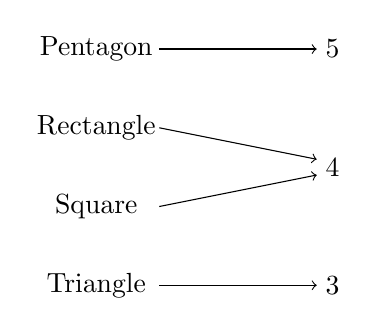
\begin{tikzpicture}
                \draw[align=right] (0, 0) node {Triangle};
                \draw[align=right] (0, 1) node {Square};
                \draw[align=right] (0, 2) node {Rectangle};
                \draw[align=right] (0, 3) node {Pentagon};
                
                \draw (3, 0.0) node {3};
                \draw (3, 1.5) node {4};
                \draw (3, 3.0) node {5};
                
                \draw [->] (0.8, 0) -- (2.8, 0.0);
                \draw [->] (0.8, 1) -- (2.8, 1.4);
                \draw [->] (0.8, 2) -- (2.8, 1.6);
                \draw [->] (0.8, 3) -- (2.8, 3.0);
            \end{tikzpicture}
            \caption{Digraph Relationship Between Polygons and the Number of Sides.}
            \label{fig:RelationshipBetweenPolygonsAndSides}
        \end{figure}
        
        Giving our relation between A and B the symbol $A \sim B$, we can also put them in a Cayley Predicate Table:
        
        \begin{table}[ht]
            \centering
            \begin{tabular}{|c|c|c|c|c|}
                \hline
                \multicolumn{2}{|c|}{\multirow{2}{*}{$A \sim B$}} & \multicolumn{3}{c|}{B} \\ \cline{3-5} 
                \multicolumn{2}{|c|}{} & 5 & 4 & 3 \\ \hline
                \multirow{4}{*}{A} & Pentagon & \cmark & \xmark & \xmark \\ \cline{2-5} 
                 & Rectangle & \xmark & \cmark & \xmark \\ \cline{2-5} 
                 & Square & \xmark & \cmark & \xmark \\ \cline{2-5} 
                 & Triangle & \xmark & \xmark & \cmark \\ \hline
            \end{tabular}
            \caption{Cayley Predicate Table of Relation Between Polynomials and Sides.}
            \label{tab:CayleyPredicateTableRelationPolynomialsSides}
        \end{table}
        
        Note from both table and digraph that $A \sim B \neq B \sim A$. In other words, it is not commutative, but we WILL discuss associativity.
        
        Discuss composition through ``matrix multiplication''. Discuss different symbolic ways to represent relations.
        
        You can notice that by looking at the Cayley Predicate Table that the checkmark (\cmark) is found exactly once per row of A. This is equivalent to saying that, on the diagraph, that there is exactly one arrow coming from each object of the shapes set.
        
        \begin{definition}
            A left-unique 
        \end{definition}
        
        A function in pure mathematics is not a function in computer science, despite that computer science is an offshoot of mathematcics (around the foundations of mathematics). The context of the word function changes in computer science to include side-effects, let's start with state and then go to sessions.
    
        Unary relations are set comprehensions
        \begin{section}{Function-Like Relations}
        \end{section}
        
        \begin{section}{Order-like Relations}
        
        \end{section}
        
        \begin{section}{Equivalence Relations}
        \end{section}
    \end{chapter}
    \begin{chapter}{Counting and Combinatorics}
        \begin{section}{adsf}
            \begin{subsection}{Relationships on the Boolean Algebra}
                \begin{align*}
                    |A \cap B| \leq |A| \quad  \textrm{and} \quad  |A \cap B| \leq |B|
                \end{align*}
                
                This is directly related to the fact that:
                \begin{align*}
                    X \subseteq Y \implies |X| \leq |Y|
                \end{align*}
                
                And this connection between these two, as important as it is, will be more thoroughly described later.
            \end{subsection}
            \begin{subsection}{Addition and the Disjoint Union}
            $$
                |A \sqcup B| = |A| + |B|
            $$
            \end{subsection}
            \begin{subsection}{Multiplication and the Cartesian Product}
            $$
                |A \times B| = |A| \times |B|
            $$
            \end{subsection}
            \begin{subsection}{Functions and Exponentials}
            $$
                |A \to B| = |B|^{|A|}
            $$
            \end{subsection}
            \begin{subsection}{Powerset as a Function}
            $$
                |\mathcal{P}(X)| = | X \to \mathbb{B} | = 2^{|X|}
            $$
            \end{subsection}
            \begin{subsection}{Permutations}
                Number of permutations = number of total orders ($|A|! = n!$)
            \end{subsection}
        \end{section}
    \end{chapter}
    \begin{chapter}{Probability Theory as a Logic}
    \end{chapter}
\end{part}
\begin{part}{Relations}
    \begin{chapter}{Binary Relations}
        \begin{section}{Heterogenous and Homogeneous Relations}
            Homogeneous means same-type, and heterogenous means different-type. In this regard, 
            
            Oftentimes, mathematically, we don't have specific words that mean possibly one and possibly the other. This is important, because a heterogenous relation can be homogenous too. The phrase non-homogenous specifically refers to a relation that must have different types.
        \end{section}
        
        \begin{section}{Heytingness}
            Make binary relation as ``included subsets'' ($R \in U\times V$) to a functional predicate for inclusion ($R : U \times V \to \mathbb{B}$) and that corresponds to ($R:U\to V \to \mathbb{B}$).
        \end{section}
        
        \begin{section}{asdf}
        \end{section}
    \end{chapter}
    
    \begin{chapter}{n-ary Relations}
    
    \end{chapter}
    
    \begin{chapter}{Relation Algebra}
    
    \end{chapter}
    
    \begin{chapter}{Other}
        A filter is a unary relation (can be useful as base-case in inductive arguments)
        
        A unary relation is a filter on a set (a subset)
        
        There are only 2 nullary relations: always holding and never holding
        
        A binary relation is a subset of the cartesian product
        
        A ternary relation requires an ordered n-tuple, since cartesian products are not associative. However, ((a, b), c) is also valid for discussion.
        
        
    \end{chapter}
\end{part}  
\begin{part}{Lambdas and Type Theory}
    \begin{chapter}{Lambdas and Combinators}
        Given our definition of functions in mathematics, we can define the truth-values of true and false as a choice. (describe by sentences and if/then).
        
        Then, we can define functions that allow us to select the first or the second part of the sentence:
        
        \begin{lstlisting}[language=Lambda]
            T x y = x
            F x y = y
        \end{lstlisting}
        
        \begin{lstlisting}[language=Lambda]
fix fib : int -> int.
  lambda n : int.
    if (n < 2) then n$^2$
    else (fib (n-1)) (fib (n-2))
\end{lstlisting}
        
        Then, the T function selects the first value, and the F function selects the second. It could just as well be called first and second, but we will define those later for a different purpose, and it will make less sense that this has anything to do with logic.
        
        Now, binding variables, in a way similar to quantifiers, we can define functions using lambdas, we will start with a function called the identify function, that gives you whatever you put in:
        
        \begin{lstlisting}[language=Lambda]
            I x = x
            I = lambda x.x
        \end{lstlisting}
        
        That is to say that the function I (again, standing for identity) is a function that takes a parameter x and returns that same argument.
        
        You will notice that instead of a symbol indicating set membership ($\in$), we separate the variable binding from the expression with the period.
        
        It may seem silly at first to have an alternative way to define a function, but the important thing is that we are not always interested in naming all of our functions. However, that's not the only benefit, the next benefit will come about as we keep talking.
        
        For now, let's define our true and false functions from before, rewriting them into lambda terms:
        
        \begin{lstlisting}[language=Lambda]
            T x y = x      T = lambda x.(lambda y.x)
            F x y = y      F = lambda x.(lambda y.y)
        \end{lstlisting}
        
        Now, again, this looks like it's creating more work, and if the goal was to express things with the least number of symbols possible, then we'd be failing. Instead. we are attempting to construct something, and the ideas will become more clear as we begin to make use of it.
        
        To apply an argument to a function looks like the following:
        
        \begin{lstlisting}[language=Lambda]
            T 3 5 = lambda x.(lambda y.x) 3 5
            T 3 5 =     (lambda y.3)   5
            T 3 5 =          3
        \end{lstlisting}
        
        The first action for application is to substitute x (the first parameter) with 3 everywhere it is used (which just so happens to be inside the parentheses). The second action is to substitute y with 5 everywhere y is found (which is not found anywhere.
        
        First things first, I want to talk about more standard order of operation (or probably more specific, ``order of interpretation'' in this case). Lambda abstractions are interpreted as right-associative, meaning that the definitions above are equivalent to:
        
        \begin{lstlisting}[language=Lambda]
            T = lambda x . lambda y . x
            F = lambda x . lambda y . y
        \end{lstlisting}
        
        \todo{discuss how this introduces us to functions that return functions}
        \todo{discuss the equivalence of this to the tuple form}
        
        Now, regarding the other operators that we'd expect from a Boolean data type, we'd expect to be able to interpret logical negation (NOT). In this case, if we logically negate the value, we swap T with F (and vice versa), which is equivalent to swapping which of the two values are selected. For instance, we'd expect the following:
        
        \begin{lstlisting}[language=Lambda]
            NOT T x y = y
            NOT F x y = x
        \end{lstlisting}
        
        So, a way that we could do this is to swap x and y:
        
        \begin{lstlisting}[language=Lambda]
            NOT p x y = p y x
        \end{lstlisting}
        
        If we used the same parameters as before, accepting T as the function that would be used:
        
        \begin{lstlisting}[language=Lambda]
            NOT T 3 5 = T 5 3
                      =   5
        \end{lstlisting}
        
        Notice that we can demonstrate the following:
        
        \begin{lstlisting}[language=Lambda]
            NOT T x y = T y x = y
                      = F x y = y
                
            NOT F x y = F y x = x
                      = T x y = x
        \end{lstlisting}
        
        So, we can say that applying NOT to T and F would give the same computed results as:
        \begin{lstlisting}[language=Lambda]
            NOT T = F
            NOT F = T
        \end{lstlisting}
        
        
    \end{chapter}
    
    \begin{chapter}{Types}
        \begin{section}{As a Pseudocomplemented Lattice}
            We discussed how function types act like the implication of a logic. Referring back to Order Theory, we also discussed Heyting Algebras and Pseudocomplements, and how the great thing about having a bounded semilattice was that we could generate a pseudocomplement from the bound.
        
            We assume that the upper bound is off limits in order to avoid Russell's Paradox on Types. However, we can attempt to find a lower-bound and use that instead. We need something that no type can be less than. Our first guess may be the unit type, but that still may not be the best type.
        
            Remember that a unit type can be passed to a function, and it can be returned from a function and then used. Imagine instead a type that cannot be constructed, and therefore it cannot return. We will call this type ``absurdity'' and it will be the bottom-element. This also means that we will often refer to it as the bottom type, and we will give it the symbol $\bot$.
        
            Therefore, we can also define our pseudocomplement (our negation) as a function that returns the bottom type: $A \to \bot$. Effectively, returning $\bot$ would be evidence that the program cannot compile (i.e. our proof fails). However, some programs are required to run forever, and so there may be situations where not returning is the correct behavior.
        
            With that out of the way, let's discuss the other property of a Heyting Algebra, that a monoid exists such that $c\wedge a \leq b \iff c \leq a \to b$. With the understanding that the $\leq$ actually means $\to$, we are looking for what meaning of $\wedge$ causes $c\wedge a \to b \iff c \to a \to b$.
        
            We have discussed previously that, when working with functions, we can call a function by $(A \times B) \to C$ or we can call it as $A \to (B \to C)$. This cartesian product is precisely the $\wedge$ we are looking for.
        
            This means that we have all the connections between the following:
            \begin{itemize}
                \item Boolean Logic (Heyting Algebras) -- $[(A\ \wedge\ B) \implies C] \iff [A \implies (B \implies C)]$
                \item Algebra -- $(c^{b})^{a} = c^{ba}$
                \item Type Theory / Functions -- $(A\times B) \to C \iff A \to (B \to C)$
                \item Category Theory -- $Hom(A \otimes B, C) = Hom(A, B \Rightarrow C)$
            \end{itemize}
        \end{section}
        \begin{section}{The Coproduct}
            We have defined the product in Type Theory now, and as we have stated, when there is a product, there is a coproduct in the opposite category. Well, we're going to skip the full categorical dual and continue discussing the relationships with the Heyting Algebra from before.
            
            Remember that, algebraically, when we have an exponential, we get the property that $(c^a)(c^b) = c^{a + b}$. It so happens that in logic, this also takes the same form that the join has: $(a \implies c) \wedge (b\implies c) \iff (a \vee b) \implies c$.
            
            So, we are looking for how to interpret $(A \to C) \times (B \to C)$, which are 2 functions, that allow us to get a type $C$ based on whether the input is $A$ or the input is $B$. In this regard, it's a choice between the inputs A and B. This has some characteristics similar to our disjoint union from set theory.
            
            We turn a proof of $A + B$ into a proof of $A$ or a proof of $B$, either of which allows us to get to $C$.
            
            In fact, we have a very perfect example of such a disjoint union available at hand:
            $$
                \mathbb{B} = T \vert F
            $$
            
            Where the ($\vert$) symbol means ``select between'', and being that T is a unit type (1), and F is also a unit type (1), then $\mathbb{B} = 1 + 1$ is sometimes denoted $2$.
        \end{section}
        \begin{section}{Peano Again}
            Now we are in a position to start defining Peano Arithmetic in Type Theory instead of plain ole Lambda Calculus. For that, we get the following:
            
            \begin{lstlisting}[language=Lambda]
                Nat = Z | S Nat
            \end{lstlisting}
            
            That is, we have the Natural Numbers defined as something that starts with zero (Z) and allows us to select a successor function (S) that takes a Natural Number as an input.
        \end{section}
    \end{chapter}
\end{part}

%----------------------------------------------------------------------------------------
%	CHAPTER 1
%----------------------------------------------------------------------------------------

\chapterimage{head2.png} % Chapter heading image

\chapter{Introduction}

\section{Motivation}\index{Motivation}
This book is a high-speed walk through the core mathematics and usages for various applications within science and engineering. It does not serve to teach proofs, or instruct on why the information contained herein works the way that it does, but instead serves to move straight to the heart of application.

The point of this book is to treat everything as computation. We will study arithmetic computations, algebraic computations, infinitesimal calculus, a calculus of sets, probability theory, statistics, etc. Until we have thoroughly gone through many of the most industry useful methodology.

The problem with this book is that it will make mathematics look as if it is about manipulating symbols in kind of ``mathematical language''. The duty and work of mathematicians was to create a system where it was possible that such symbolic manipulation is possible.

Worse yet, it allows one to forget that mathematicians are actively busy coming up with new things all the time. However, it's not the goal of this book to convince the reader of that. There are additional books in the series that are tuned to explaining just how we got where we are, and where we are going.

\chapter{Algebra/Working with Expressions}
The biggest difference between arithmetic and algebra is that arithmetic was interested in working with values and performing calculations on them. Algebraic manipulation is very effective, because there are plenty of things that can be put into an algebraic context, and then manipulated the way that we manipulate algebraic expressions.
\section{Expressions}
\begin{definition}{Expression}
A mathematical expression is a well-formed collection of symbols arranged according to rules called \textbf{syntax}.
\end{definition}

The symbols may represent operations, constants, variables, functions, brackets, etc. The brackets typically explicitly give the order of operations for the expression. When the symbols are omitted, a standard order of operations are accepted.

\section{Order of operations}
In order to understand the order of operations, it's important to start with the natural numbers.

\begin{remark}
    Natural numbers are the \emph{only} type of object where multiplication is repeated addition, and where exponentiation is repeated multiplication.
\end{remark}

This is only a means of remembering the order of operation, and is not directly a reason for how the order of operations became a commonly used standard. However, the definition, going into addition, multiplication, and exponentiation separate these operations into the following levels:

\begin{tabular}{|l|l|l|l|} \hline
Level & Action & Inverse Action \\ \hline
1 & Addition & Subtraction \\ \hline
2 & Multiplication & Division \\ \hline
3 & Exponentiation & \\ \hline
4 & Function Application & \\ \hline
5 & Brackets & \\ \hline
\end{tabular}

Therefore, if one gets the following expression, where $x=5$:

\begin{equation}
2(x-1)^3+\log(5+x)=0
\end{equation}

One works left-to-right, but starts with the highest level expressions first:

\begin{equation}
\begin{aligned}
2(5-1)^3+\log(5+5)& = 0 & \textsf{Expression with Substitution} \\
2(4)^3+\log(10)&=0 &\textsf{Brackets} \\
2(4)^3+1&=0&\textsf{Function Application} \\
2(64)+1&=0&\textsf{Exponentiation} \\
128+1&=0&\textsf{Multiplication} \\
129&=0&\textsf{Addition}
\end{aligned}
\end{equation}

\section{How to look at algebra}
For equations, we have the rule that, for any expression $x=y$ and any function ``f'':


Demonstrate to reader how this next equation is a consequence of equivalence classes...
\begin{equation}
x=y \Leftrightarrow f(x)=f(y)
\end{equation}

\part{Topics}
Foundational parts
\begin{itemize}
    \item Categories (logic and order)
    \item Model Theory (sets, types, etc.)
    \item Algebraic Theories (axiomatic definitions and symbolic manipulations through orders)
    \item Topology (including calculus)
\end{itemize}


\begin{itemize}
    \item The different meanings of equality: isomorphism vs identity
    \item Multiplication and addition as more fundamental than division or subtraction, with the exception of how subtraction is actually a distance function
    \url{https://www.quora.com/Do-we-need-division-and-subtraction-as-separate-operations-when-division-can-be-written-as-a-factor-with-the-exponent-of-1-and-subtraction-of-a-term-as-an-addition-of-the-negative-term-a-div-b-a-cdot-frac-1-b-a-b-a/answer/Nicholas-Cooper-8}
    
    \item That imaginary numbers are as imaginary as real numbers:
    \url{https://www.quora.com/Are-all-numbers-really-imaginary-numbers-How-are-numbers-real/answer/Nicholas-Cooper-8}
    \url{https://www.quora.com/What-real-world-phenomena-can-be-quantified-with-imaginary-numbers/answer/Nicholas-Cooper-8}
    
    \item The truth about measurements
    \url{https://www.quora.com/A-scalar-quantity-can-t-be-negative-because-it-only-has-magnitude-but-no-direction-but-why-can-temperature-can-be-negative/answer/Nicholas-Cooper-8}
    
    
\end{itemize}


%----------------------------------------------------------------------------------------
%	CHAPTER 3
%----------------------------------------------------------------------------------------
\printglossaries
\end{document}